\documentclass{article}

\usepackage{amsmath}
\usepackage{amssymb}
\usepackage{amsthm}
\usepackage{enumitem}
\usepackage{booktabs}
\usepackage{caption}
\usepackage{nicematrix}
\usepackage{graphicx}
\usepackage{tcolorbox}
\usepackage{siunitx}
\usepackage{cancel}
\usepackage{listings}
\usepackage{aligned-overset}
\usepackage{tikz}
\usepackage{./chapters/mycolors}
\usepackage{nicematrix}
\usepackage{hyperref}

\newcounter{exctr}[section]
\labelformat{exctr}{\thesection.\arabic{exctr}}

\newenvironment{exercise}{
    \refstepcounter{exctr}\trivlist{}
    \item\relax\textbf{Exercise \thesection.\theexctr} 
}{\endtrivlist}

\newenvironment{solution}{\trivlist{}\item\relax\textit{Solution:}}{\endtrivlist}

\newtheorem{theorem}{Theorem}

\newcommand{\bsum}[1][n]{\sum_{#1=0}^\infty}
\newcommand{\infsum}[1][n]{\sum_{#1=-\infty}^\infty}
\newcommand{\expcoeff}{\frac{x^n}{n!}}
\newcommand{\coeff}[1]{\left[#1\right]}

\DeclareMathOperator{\prob}{Prob}
\DeclareRobustCommand{\stirlingFst}{\genfrac[]{0pt}{}}
\DeclareRobustCommand{\stirlingSnd}{\genfrac\{\}{0pt}{}}

\newcommand*\diff{\mathop{}\!\mathrm{d}}

\newcommand{\estep}[1]{\overset{#1}{=}}
\newcommand{\estepalign}[1]{\overset{#1}&{=}}


\setlist{  
  listparindent=\parindent
}

\lstdefinelanguage{Maple}%
{morekeywords={and,assuming,break,by,catch,description,do,done,%
elif,else,end,error,export,fi,finally,for,from,global,if,%
implies,in,intersect,local,minus,mod,module,next,not,od,%
option,options,or,proc,quit,read,return,save,stop,subset,then,%
to,try,union,use,uses,while,xor},%
sensitive=true,%
morecomment=[l]\#,%
morestring=[b]",%
morestring=[d]"%
}[keywords,comments,strings]%

\definecolor{lightgray2}{rgb}{0.95, 0.95, 0.95}
\lstnewenvironment{mapleinput}{%
  \lstset{
    language=Maple, 
    backgroundcolor=\color{lightgray2}, 
    basicstyle=\ttfamily, 
    escapechar=\%,
    keepspaces=true
  }
}{}

\newenvironment{mapleoutput}{%
  \color{blue}\ttfamily
}{}

\newcommand{\prompt}{\textcolor{purple}{>}}

\newcommand\crule[3][black]{\textcolor{#1}{\rule{#2}{#3}}}
\newcommand{\hl}[2]{\colorbox{#1}{\strut \ensuremath{#2}}}

\title{generatingfunctionology solutions}
\author{Jan Quan}
\date{\today}

\begin{document}
    \maketitle
    \section*{List of formulas}
\subsection*{Power series}
\begin{equation} \label{eq:power_geom}
    \frac{1}{1-x} = \bsum x^n
\end{equation}
\begin{equation} \label{eq:power_loggeom}
    \log \frac{1}{1-x} = \sum_{n=1}^{\infty} \frac{x^n}{n}
\end{equation}
\begin{equation} \label{eq:power_exp}
    e^x = \bsum \frac{x^n}{n!}
\end{equation}
\begin{equation} \label{eq:power_sin}
    \sin x = \bsum (-1)^n \frac{x^{2n+1}}{(2n+1)!}
\end{equation}
\begin{equation} \label{eq:power_cos}
    \cos x = \bsum (-1)^n \frac{x^{2n}}{(2n)!}
\end{equation}
\begin{equation} \label{eq:power_sinh}
    \sinh x = \bsum \frac{x^{2n+1}}{(2n+1)!}
\end{equation}
\begin{equation} \label{eq:power_cosh}
    \cosh x = \bsum \frac{x^{2n}}{(2n)!}
\end{equation}
\begin{equation} \label{eq:binom_num}
    (1+x)^{\alpha} = \infsum[k] \binom{\alpha}{k}x^k
\end{equation}
\begin{equation} \label{eq:binom_num2}
    (x+y)^{\alpha} = \infsum[k] \binom{\alpha}{k}y^kx^{\alpha - k}
\end{equation}
\begin{equation} \label{eq:binom_denom}
    \frac{1}{(1-x)^{k+1}} = \infsum \binom{n+k}{n}x^n
\end{equation}
\begin{equation} \label{eq:binom_denom_num_single}
    \frac{x^k}{(1-x)^{k+1}} = \bsum[r] \binom{r}{k}x^r, \quad k\in\mathbb{N}
\end{equation}
\begin{equation} \label{eq:power_bernoulli}
    \frac{x}{e^x-1} = \bsum \frac{B_nx^n}{n!}
\end{equation}
\begin{equation} \label{eq:power_tan_inv}
    \tan^{-1}x = \bsum (-1)^n \frac{x^{2n+1}}{2n+1}
\end{equation}
\begin{equation} \label{eq:power_catalan_1}
    \frac{1}{2x}(1-\sqrt{1-4x}) = \infsum[n] \frac{1}{n+1} \binom{2n}{n}x^n 
\end{equation}
\begin{equation} \label{eq:power_catalan_2}
    \frac{1}{\sqrt{1-4x}} = \infsum[k] \binom{2k}{k}x^k
\end{equation}
\begin{equation} \label{eq:stSnd}
    \frac{x^k}{(1-x)(1-2x)\cdots (1-kx)} = \bsum \stirlingSnd{n}{k}x^n
\end{equation}
\begin{align} \label{eq:power_tan}
    \tan x &= \sum_{r=1}^\infty (-1)^{r-1}\frac{2^{2r}(2^{2r}-1)B_{2r}}{(2r)!}x^{2r-1} \\
    &=  x + \frac{x^3}{3} + \frac{2x^5}{15} + \frac{17x^7}{315} + \frac{62x^9}{2835} + \ldots \notag
\end{align}
\begin{align} \label{eq:power:xcot}
    x\cot x &= \bsum[k] \frac{(-4)^kB_{2k}}{(2k)!}x^{2k} \\
    &= 1-\frac{x^2}{3} - \frac{x^4}{45} - \frac{2x^6}{945} - \frac{x^8}{4725} - \ldots \notag
\end{align}

\subsection*{Common Identities and Theorems}
\begin{equation} \label{eq:xD} \tag{$xD$}
    (xD) x^n = nx^n, \quad  n \in \mathbb{N} \quad (D \textnormal{ denotes derivative})
\end{equation}
\begin{equation} \label{eq:bin_sym}
    \binom{n}{k} = \binom{n}{n-k}, \quad  k\in\mathbb{Z}, n \in\mathbb{N} 
\end{equation}
\begin{equation} \label{eq:div_swap}
    \sum_{d\vert n} f(d) = \sum_{d\vert n} f\left(\frac{n}{d}\right), \quad  n \in\mathbb{N}
\end{equation}
\begin{equation} \label{eq:power_zeta}
    \zeta(s) = \sum_{n=1}^\infty \frac{1}{n^s} = \prod_{\textnormal{$p$ prime}} \frac{1}{1-p^{-s}}
\end{equation}
\begin{equation} \label{eq:sieve} \tag{sieve}
    E(x) = N(x-1), \quad (\textnormal{See Chapter 4.2})
\end{equation}
\begin{equation} \label{eq:binom_asymp}
    \binom{n-\alpha-1}{n} \approx \frac{n^{-\alpha-1}}{\Gamma(-\alpha)} \left[1 + \frac{\alpha(\alpha +1)}{2n} + \frac{\alpha(\alpha+1)(\alpha+2)(3\alpha+1)}{24n^2} + \cdots\right]
\end{equation}
\begin{theorem} \label{thm:conv_power}
    There exists a number $R$, $0\leq R \leq +\infty$, called the radius of convergence of the series $f$, such that the series converges for all values of $z$ with $|z|<R$ and diverges for all $z$ such that $|z|>R$. The number $R$ is expressed in terms of the sequence $\{a_n\}_0^\infty$ of coefficients of the series by means of
    \[
        R = \frac{1}{\limsup_{n\to\infty} |a_n|^{1/n}} \qquad (1/0=\infty;\ 1/\infty = 0).
    \]
\end{theorem}
\begin{theorem} \label{thm:euler_prod}
    Let $f$ be a multiplicative number-theoretic function. Then we have the formal identity
    \[
        \sum_{n=1}^\infty \frac{f(n)}{n^s} = \prod_p \left\{1+f(p)p^{-s} + f(p^2)p^{-2s} + f(p^3)p^{-3s} + \cdots\right\}
    \]
    in which the product on the right extends over all prime numbers $p$.
\end{theorem}
\begin{theorem} \label{thm:lif}
    \textbf{(The Lagrange inversion formula.)} Let $f(u)$ and $\phi(u)$ be formal power series in $u$, with $\phi(0)=1$. Then there is a unique formal power series $u=u(t)$ that satisfies $u=t\phi(u)$. Further, the value $f(u(t))$ of $f$ at that root $u=u(t)$, when expanded in a power series in $t$ about $t=0$, satisfies
    \[
        \coeff{t^n} {f(u(t))} = \frac{1}{n}\coeff{u^{n-1}} {f'(u)\phi(u)^n}.
    \]
\end{theorem}
\begin{theorem} \label{thm:darboux}
    \textbf{(Darboux)} Let $v(z)$ be analytic in some disk $|z|<1+\eta$, and suppose that in a neighborhood of $z=1$ it has the expansion $v(z) = \bsum[j] v_j(1-z)^j$. Let $\beta\notin\{0,1,2,\ldots\}$. Then
    \begin{align*}
        \coeff{z^n}\{(1-z)^\beta v(z)\} &= \coeff{z^n} \left\{\sum_{j=0}^m v_j(1-z)^{\beta+j}\right\} + \mathcal{O}(n^{-m-\beta-2}) \\
        &= \sum_{j=0}^m v_j \binom{n-\beta -j-1}{n} + \mathcal{O}(n^{-m-\beta-2}).
    \end{align*}
\end{theorem}
\begin{theorem} \label{thm:hayman}
    \textbf{(Hayman)} Let $f(z)=\sum a_nz^n$ be an admissible function. Let $r_n$ be the positive real root of the equation $a(r_n)=n$, for each $n=1,2,\ldots,$ where $a(r)=r \frac{f'(r)}{f(r)}$. Then
    \[
        a_n \sim \frac{f(r_n)}{r_n^n\sqrt{2\pi b(r_n)}} \qquad \textnormal{as $n\to+\infty,$}
    \]
    where $b(r)=ra'(r)$.
\end{theorem}
 \newpage
    \section{Introductory Ideas and Examples}
\begin{exercise} \label{ex:1-1}
    Find the ordinary power series generating functions of each of the following sequences, in simple, closed form. In each case the sequence is defined for all $n \geq 0$.
    \begin{enumerate}[label=(\alph*)]
        \item $a_n = n$
        \item $a_n = \alpha n + \beta$
        \item $a_n = n^2$
        \item $a_n = \alpha n^2 + \beta n + \gamma$
        \item $a_n = P(n)$, where $P(n)$ is a given polynomial, of degree $m$.
        \item $a_n = 3^n$
        \item $a_n= 5\cdot 7^n - 3\cdot 4^n$
    \end{enumerate}
\end{exercise}

\begin{solution}
    For each of the sequences, define $A(x) = \bsum a_n x^n$, then apply following steps.
    \begin{enumerate}
        \item Multiply both sides of the sequence definition by $x^n$ and sum over all $n \geq 0$.
        \item The left-hand side is recognized as $A(x)$.
        \item Express the right-hand side using known power series.
    \end{enumerate}

    \begin{enumerate}[label=(\alph*)]
        \item \hypertarget{eq:ch1:1:a}{} Apply $xD$ trick and bring the $xD$ outside.
            \[
                A(x) = \bsum n x^n \estep{\eqref{eq:xD}} \bsum xDx^n = xD\bsum x^n \overset{\eqref{eq:power_geom}}{=} xD\frac{1}{1-x} = \frac{x}{(1-x)^2}
            \] 
        \item \hypertarget{eq:ch1:1:b} Split the sum and handle each part separately.
            \[
                A(x) = \bsum \alpha n x^n + \bsum\beta x^n \estep{\hyperlink{eq:ch1:1:a}{1.1(a)},\eqref{eq:power_geom}} \frac{\alpha x}{(1-x)^2} + \frac{\beta}{1-x}
            \]
        \item Apply the $xD$ trick twice.
        \[
            A(x) = \bsum n^2x^n \estep{\eqref{eq:xD}} \bsum (xD)^2x^n \estep{\eqref{eq:power_geom}} (xD)^2 \frac{1}{1-x} = \frac{x+x^2}{(1-x)^3}
        \]
        \item A combination of the results from the previous parts.
        \[
            A(x) = \bsum \left(\alpha n^2 x^n + \beta n x^n + \gamma x^n \right) \estep{\hyperlink{eq:ch1:1:b}{1.1(b\text{-}c)}} \frac{\alpha x +\alpha x^2}{(1-x)^3} + \frac{\beta x}{(1-x)^2} + \frac{\gamma}{1-x}
        \]
        \item \hypertarget{eq:ch1:1:e} Let $P(n) = c_m n^m + c_{m-1} n^{m-1} + \ldots + c_1 n + c_0 $ and apply $xD$ trick multiple times.
        \begin{align*}
            A(x) &= \bsum \left(c_m n^m  + c_{m-1} n^{m-1}  + \ldots + c_1 n + c_0 \right)x^n \\
            \estepalign{\eqref{eq:xD}} (c_m (xD)^m + c_{m-1}(xD)^{m-1} + \ldots + c_0) \bsum x^n  \estep{\eqref{eq:power_geom}} P(xD) \frac{1}{1-x}
        \end{align*}
        \item
        \[
            A(x) = \bsum 3^n x^n = \bsum (3x)^n \estep{\eqref{eq:power_geom}} \frac{1}{1-3x}
        \]
        \item
        \[
            A(x) = 5\bsum (7x)^n - 3 \bsum (4x)^n \estep{\eqref{eq:power_geom}} \frac{5}{1-7x} - \frac{3}{1-4x}
        \]
    \end{enumerate}
\end{solution}

\begin{exercise} \label{ex:1-2}
    For each of the sequences given in Exercise~\ref{ex:1-1}, find the exponential generating function of the sequence in simple, closed form.
\end{exercise}
\begin{solution}
    For each of the sequences, define $A(x) = \bsum a_n \expcoeff$, then apply the method from the previous exercise but where $x^n$ is replaced by $\expcoeff$ in the first step.
    \begin{enumerate}[label=(\alph*)]
        \item \hypertarget{eq:ch1:2:a}
        \[
            A(x) = \bsum n\frac{x^n}{n!} \estep{\eqref{eq:xD}} \bsum xD \frac{x^n}{n!} = xD \bsum \frac{x^n}{n!} \estep{\eqref{eq:power_exp}} xD e^x = x e^x
        \]
        \item \hypertarget{eq:ch1:2:b} Split sum.
        \[
            A(x) = \bsum \alpha n \frac{x^n}{n!} + \bsum\beta \frac{x^n}{n!} \estep{\hyperlink{eq:ch1:2:a}{1.2(a)},\eqref{eq:power_exp}} \alpha x e^x + \beta e^x
        \]
        \item $xD$ trick twice.
        \[
            A(x) = \bsum n^2\frac{x^n}{n!} \estep{\eqref{eq:xD}} (xD)^2 \bsum \frac{x^n}{n!} \estep{\eqref{eq:power_exp}} (xD)(xe^x)= (x+x^2)e^x
        \]
        \item Combination of previous results.
        \[
            A(x) = \bsum \alpha n^2 \frac{x^n}{n!} + \beta n \frac{x^n}{n!} + \gamma \frac{x^n}{n!} \estep{\hyperlink{eq:ch1:2:b}{1.2(b\text{-}c)}}  \alpha (x + x^2)e^x + \beta xe^x + \gamma e^x
        \]
        \item Analogous to its Exercise~\ref{ex:1-1} counterpart.
        \[
            A(x) = (c_m(xD)^m + \ldots + c_1(xD) + c_0)\bsum \frac{x^n}{n!} \estep{\eqref{eq:power_exp}} P(xD)e^x
        \]
        \item
        \[
            A(x) = \bsum 3^n \frac{x^n}{n!} = \bsum \frac{(3x)^n}{n!} \estep{\eqref{eq:power_exp}} e^{3x}
        \]
        \item
        \[
            A(x) = 5\bsum \frac{(7x)^n}{n!} - 3 \bsum \frac{(4x)^n}{n!} \estep{\eqref{eq:power_exp}} 5e^{7x} - 3e^{4x}
        \]
    \end{enumerate}
\end{solution}

\begin{exercise}
    \label{ex:1-3}
    If $f(x)$ is the ordinary power series generating function of the sequence $\{a_n\}_{n\geq 0}$, then express simply, in terms of $f(x)$, the ordinary power series generating functions of the following sequences. In each case the range of $n$ is $0$, $1$, $2$, $\ldots$
    \begin{enumerate}[label=(\alph*)]
        \item $\{a_n + c\}$
        \item $\{\alpha a_n + c\}$
        \item $\{na_n\}$
        \item $\{P(n)a_n\}$, where $P$ is a given polynomial.
        \item $0, a_1, a_2, a_3, \ldots$
        \item $0, 0, 1, a_3, a_4, a_5, \ldots$
        \item $a_0, 0, a_2, 0, a_4, 0, a_6, 0, a_8, 0, \ldots$
        \item $a_1, a_2, a_3, \ldots$
        \item $\{a_{n+h}\}$ \quad ($h$ a given constant)
        \item $\{a_{n+2}+3a_{n+1}+a_n\}$
        \item $\{a_{n+2} - a_{n+1} - a_{n}\}$
    \end{enumerate}
\end{exercise}
\begin{solution}
    Let $g(x)$ be the ordinary power series of the desired sequences. The results follow from simple algebraic manipulations.
    \begin{enumerate}[label=(\alph*)]
        \item Split sum.
        \[
            g(x) =  \bsum (a_n + c) x^n= \bsum a_n x^n + c\bsum x^n \estep{\eqref{eq:power_geom}} f(x) + \frac{c}{1-x}
        \]
        \item Completely analogous as previous part.
        \[
            g(x) = \bsum (\alpha a_n +c) x^n = \alpha \bsum a_n x^n + c \bsum x^n \estep{\eqref{eq:power_geom}} \alpha f(x) + \frac{c}{1-x}
        \]
        \item \hypertarget{eq:ch1:3:c}{} $xD$ trick.
        \[
            g(x) = \bsum na_n x^n 
            \estep{\eqref{eq:xD}} xD \bsum a_n x^n 
             = xDf(x)
        \]
        \item \hypertarget{eq:ch1:3:d}{} Same method as \hyperlink{eq:ch1:1:e}{1.1(e)}.
        \[
            g(x) = \bsum (c_m (xD)^m + \ldots + c_1 (xD) + c_0)a_nx^n = P(xD)f(x)
        \]
        \item \hypertarget{eq:ch1:3:e} Add and subtract $a_0$ to become $f(x)$.
        \[
            g(x) = \sum_{n=1}^\infty a_n x^n =  -a_0 + \bsum a_n x^n = -a_0 + f(x) 
        \]
        \item Add and subtract $a_0 + a_1x + (a_2 - 1)x^2$.
        \[
            g(x) = -a_0 - a_1x - (a_2 - 1)x^2 + \bsum a_n x^n 
            = -a_0 - a_1x-(a_2-1)x^2 + f(x)
        \]
        \item \hypertarget{eq:ch1:3:g}{} Even part of $f(x)$.
        \begin{align*}
            g(x) &= \bsum a_{2n} x^{2n}
            = \frac{a_0}{2} + \frac{a_0}{2} + \frac{a_1}{2}x + \frac{a_1}{2}(-x) + \frac{a_2}{2}x^2+ \frac{a_2}{2}(-x)^2 + \ldots \\
            &= \bsum \frac{a_n}{2}x^n + \bsum \frac{a_n}{2} (-x)^n= \frac{f(x)}{2} + \frac{f(-x)}{2}
        \end{align*}
        \item \hypertarget{eq:ch1:3:h} Multiply and divide by $x$.
        \[
            g(x) = \bsum a_{n+1}x^n= \frac{\bsum a_{n+1}x^{n+1}}{x} =\frac{\sum_{n=1}^\infty a_nx^n}{x} \estep{\hyperlink{eq:ch1:3:e}{(e)}} \frac{-a_0 + f(x)}{x}
        \]
        \item \hypertarget{eq:ch1:3:i} Multiply and divide by $x^h$.
        \[
            g(x) = \bsum a_{n+h} x^n= \frac{\bsum a_{n+h}x^{n+h}}{x^h}= \frac{\sum_{n=h}^\infty a_{n}x^{n}}{x^h}
        \]
        Add and subtract $\sum_{n=0}^{h-1}a_nx^n$ in the numerator.
        \[
            g(x) = \frac{\bsum a_n x^n- \sum_{n=0}^{h-1} a_n x^n }{x^h}
             = \frac{f(x) - \sum_{n=0}^{h-1} a_n x^n}{x^h}
        \]
        \item The result follows from part \hyperlink{eq:ch1:3:i}{(i)} after splitting the sum.
        \begin{align*}
            g(x) &= \bsum a_{n+2}x^n + 3\bsum a_{n+1}x^n + \bsum a_n x^n  \\
            \estepalign{\hyperlink{eq:ch1:3:i}{1.3(i)}} \frac{f(x) - a_0 - a_1x}{x^2} + \frac{3f(x) - 3a_0}{x} + f(x)
        \end{align*}
        \item Completely analogous to the previous part.
        \begin{align*}
            g(x) &= \bsum a_{n+2}x^n - \bsum a_{n+1}x^n - \bsum a_n x^n \\
            \estepalign{\hyperlink{eq:ch1:3:i}{1.3(i)}} \frac{f(x) -a_0 - a_1x}{x^2} - \frac{f(x) - a_0}{x} - f(x)
        \end{align*}
    \end{enumerate}
\end{solution}

\begin{exercise} \label{ex:1-4}
    Let $f(x)$ be the \emph{exponential} generating function of a sequence $\{a_n\}$. For each of the sequences in Exercise \ref{ex:1-3}, find the exponential generating function simply, in terms of $f(x)$.
\end{exercise}
\begin{solution}
    The methodology and ideas are completely equivalent to the previous exercise. Let $g(x)$ be the exponential generating function of the desired sequence.
    \begin{enumerate}[label=(\alph*)]
        \item \[
            g(x) = \bsum (a_n + c) \frac{x^n}{n!} = \bsum a_n \frac{x^n}{n!} + c\bsum \frac{x^n}{n!} \estep{\eqref{eq:power_exp}} f(x) + ce^x
        \]
        \item \[
            g(x) = \bsum (\alpha a_n +c) \frac{x^n}{n!} = \alpha \bsum a_n \frac{x^n}{n!} + c\bsum \frac{x^n}{n!} \estep{\eqref{eq:power_exp}} \alpha f(x) + ce^x
        \]
        \item \[
            g(x) = \bsum na_n\frac{x^n}{n!} 
            \estep{\eqref{eq:xD}} (xD)\bsum a_n \frac{x^n}{n!}
            = xDf(x)
        \]
        \item \[
            g(x) = \bsum P(n) a_n \frac{x^n}{n!} \estep{\eqref{eq:xD}} P(xD) \bsum a_n \frac{x^n}{n!} = P(xD)f(x) 
        \]
        \item \hypertarget{eq:ch1:4:e} \[
            g(x) = \sum_{n=1}^\infty a_n \frac{x^n}{n!} = -a_0 + \bsum a_n \frac{x^n}{n!} = -a_0 + f(x)
        \]
        \item\[
            g(x) = \frac{x^2}{2!} + \sum_{n=3}^\infty a_n \frac{x^n}{n!} \\
            = -a_0 - a_1x - (a_2-1)\frac{x^2}{2} + f(x)
        \]
        \item \[
            g(x) = \bsum a_{2n} \frac{x^{2n}}{(2n)!} = \bsum \frac{a_n}{2} \frac{x^n}{n!} + \bsum \frac{a_n}{2} \frac{(-x)^n}{n!} = \frac{f(x)}{2} + \frac{f(-x)}{2}
        \]
        \item \hypertarget{eq:ch1:4:h}{} \[
                g(x) = \bsum a_{n+1}\frac{x^n}{n!}
            = \bsum a_{n+1} D\frac{x^{n+1}}{(n+1)!} =  D \sum_{n=1}^\infty a_n \frac{x^n}{n!}
            \]
            Now apply the result from part \hyperlink{eq:ch1:4:e}{(e)}.
            \[
                g(x) = D (-a_0 + f(x)) = Df(x) 
            \]
        \item \hypertarget{eq:ch1:4:i}{} \begin{align*}
            g(x) &= \bsum a_{n+h} \frac{x^n}{n!} = \bsum a_{n+h} D^h \frac{x^{n+h}}{(n+h)!} \\
            &= D^h \sum_{n=h}^\infty a_n \frac{x^n}{n!} = D^h \left(- \sum_{n=0}^{h-1} a_n\frac{x^n}{n!} + \bsum a_n \frac{x^n}{n!}\right)
        \end{align*}
            Because $D^h x^n = 0$ whenever $n < h$, we find:
            \[
                g(x) = D^h \bsum a_n \frac{x^n}{n!} = D^h f(x)
            \]
        \item Apply the result from part \hyperlink{eq:ch1:4:i}{(i)} of this exercise after splitting the sum.
        \begin{align*}
            g(x) &= \bsum a_{n+2}\frac{x^n}{n!} + 3 \bsum a_{n+1}\frac{x^n}{n!} + \bsum a_n \frac{x^n}{n!} \\
            \estepalign{\hyperlink{eq:ch1:4:i}{1.4(i)}} D^2f(x) + 3Df(x) + f(x)
        \end{align*}
        \item \begin{align*}
            g(x)
            &= \bsum a_{n+2}\frac{x^n}{n!} - \bsum a_{n+1}\frac{x^n}{n!} - \bsum a_n \frac{x^n}{n!} \\
            \estepalign{\hyperlink{eq:ch1:4:i}{1.4(i)}} D^2f(x) - Df(x) - f(x)
        \end{align*}
    \end{enumerate}
\end{solution}

\begin{exercise} \label{ex:1-5}
    Find 
    \begin{enumerate}[label=(\alph*)]
        \item $\coeff{x^n} e^{2x}$
        \item $\coeff{x^n/n!} e^{\alpha x}$ 
        \item $\coeff{x^n/n!} \sin x$
        \item $\coeff{x^n} \{1/((1-ax)(1-bx))\} \quad (a\neq b)$
        \item $\coeff{x^n}(1+x^2)^m$
    \end{enumerate}
\end{exercise}
\begin{solution}
    \begin{enumerate}[label=(\alph*)]
        \item \[
            \coeff{x^n}e^{2x} \estep{\eqref{eq:power_exp}} \coeff{x^n} \bsum[k] \frac{(2x)^k}{k!} = \coeff{x^n} \bsum[k] \frac{2^k}{k!}x^k = \frac{2^n}{n!}
        \]
        \item \[
            \coeff{\frac{x^n}{n!}}e^{\alpha x} \estep{\eqref{eq:power_exp}} \coeff{\frac{x^n}{n!}} \bsum[k] \frac{(\alpha x)^k}{k!} = \coeff{\frac{x^n}{n!}} \bsum[k] \alpha^k \frac{x^k}{k!} = \alpha^n
        \]
        \item
        \[
            \coeff{\frac{x^{n}}{n!}}\sin x \estep{\eqref{eq:power_sin}} \coeff{\frac{x^{n}}{n!}} \bsum[k] \frac{(-1)^k x^{2k+1}}{(2k+1)!} = \begin{cases}
                (-1)^{(n-1)/2} & \text{if $n$ is odd} \\
                0 & \text{otherwise}
            \end{cases}
        \]
        \item Apply partial fraction decomposition.
        \begin{align*}
            \coeff{x^n}\frac{1}{(1-ax)(1-bx)} &= \coeff{x^n} \frac{\frac{a}{a-b}}{1-ax} + \coeff{x^n}\frac{\frac{b}{b-a}}{1-bx} \\
            &= \frac{1}{a-b} \left(\coeff{x^n} \frac{a}{1-ax} - \coeff{x^n} \frac{b}{1-bx}\right) \\
            \estepalign{\eqref{eq:power_geom}} \frac{1}{a-b} \left(\coeff{x^n} a\bsum[k] (ax)^k - \coeff{x^n} b\bsum[k] (bx)^k \right) \\
            &= \frac{a^{n+1} - b^{n+1}}{a-b}
        \end{align*}
        \item
        \[
            \coeff{x^n}(1+x^2)^m \estep{\eqref{eq:binom_num}} \coeff{x^n} \infsum[k] \binom{m}{k} x^{2k} = \begin{cases}
                \tbinom{m}{n/2} & \text{if $n$ is even} \\
                0 & \text{otherwise}
            \end{cases}
        \]
    \end{enumerate}
\end{solution}

\begin{exercise}
    \label{ex:1-6}
    In each part, a sequence $\{a_n\}_{n\geq 0}$ satisfies the given recurrence relation. Find the ordinary power series generating function of the sequence.
    \begin{enumerate}[label=(\alph*)]
        \item $a_{n+1} = 3a_n + 2 \quad (n\geq 0;a_0=0)$
        \item $a_{n+1} = \alpha a_n + \beta \quad (n\geq 0;a_0=0)$
        \item $a_{n+2} = 2a_{n+1} - a_n \quad (n\geq 0; a_0=0; a_1=1)$
        \item $a_{n+1} = a_n / 3 +1 \quad (n \geq 0; a_0 = 0)$
    \end{enumerate}
\end{exercise}
\begin{solution}
    We use following method for all recurrences.
        \begin{enumerate}
            \item Define $f(x) = \bsum a_n x^n$.
            \item Multiply both sides by $x^n$ and sum over $n \geq 0$.
            \item Relate both sides to $f(x)$ (for example, using results from Exercise \ref{ex:1-3}).
            \item Solve for $f(x)$.
        \end{enumerate}
    \begin{enumerate}[label=(\alph*)]
        \item \[
            \bsum a_{n+1} x^n = \bsum 3a_n x^n + \bsum 2x^n
        \]
        With \hyperlink{eq:ch1:3:h}{1.3(h)} and \eqref{eq:power_geom}, we obtain
        \[
            \frac{f(x) - a_0}{x} = 3f(x) + \frac{2}{1-x} \overset{a_0=0}{\Longleftrightarrow}f(x) = \frac{2x}{(1-x)(1-3x)}
        \]
        \item \hypertarget{eq:ch1:6:b}{} Completely analogous as the previous part.
        \[
            \bsum a_{n+1} x^n = \bsum \alpha a_n x^n + \bsum \beta x^n
        \]
        \[
            \overset{\hyperlink{eq:ch1:3:h}{(h)},\eqref{eq:power_geom}}{\Longleftrightarrow} \frac{f(x) - a_0}{x} = \alpha f(x) + \frac{\beta}{1-x} \overset{a_0=0}{\Longleftrightarrow}  f(x) = \frac{\beta x}{(1-x)(1-\alpha x)}
        \]
        \item 
        \[
            \bsum a_{n+2}x^n = \bsum 2a_{n+1}x^n - \bsum a_n x^n
        \]
        \[
            \overset{\hyperlink{eq:ch1:3:i}{(i)},\eqref{eq:power_geom}}{\Longleftrightarrow} \frac{f(x) - a_0 - a_1x}{x^2} = 2\frac{f(x) - a_0}{x} - f(x) \stackrel{\substack{a_0=0\\a_1=1}}{\Longleftrightarrow} f(x) = \frac{x}{(1-x)^2}
        \]
        \item Follows immediately from \hyperlink{eq:ch1:6:b}{1.6(b)} with $\alpha=\frac13$ and $\beta=1$.
        \[
            f(x) = \frac{3x}{(1-x)(3-x)}
        \]
    \end{enumerate}
\end{solution}

\begin{exercise}
    Give a direct combinatorial proof of the recurrence 
    \[
        b(n) = \bsum[k] \binom{n-1}{k}b(k) \quad (n\geq 1;\ b(0)=1),
    \]
    as follows: given $n$; consider the collection of all partitions of the set $[n]$. There are $b(n)$ of them. Sort out this collection into piles numbered $k=0,1,\ldots,n-1$, where the $k$th pile consists of all partitions of $[n]$ in which the class that contains the letter `$n$' contains exactly $k$ other letters. Count the partitions in the $k$th pile, and you'll be all finished.
\end{exercise}
\begin{solution}
    The $k$th pile has size
    \[
        \binom{n-1}{k}b(n-k-1)
    \]
    since there are $\binom{n-1}{k}$ ways to choose the $k$ other letters in the same class as~$n$ and $b(n-k-1)$ ways to partition the other letters. Summing over all piles gives:
    \[
        b(n) = \sum_{k=0}^{n-1} \binom{n-1}{k} b(n-k-1)  = \sum_{k=0}^{n-1} \binom{n-1}{n-k-1} b(k)
    \]
    where the last equality follows from reversing the order of summation. Using the symmetry of the binomial coefficients \eqref{eq:bin_sym} and extending the range of the summation (since the binomial coefficient $\binom{n-1}{k}$ is zero for $k > n - 1$) gives the desired recurrence relation
    \[
        b(n) = \bsum[k] \binom{n-1}{k}b(k).
    \]
\end{solution}

\begin{exercise} \label{ex:1-8}
    In each part of Exercise \ref{ex:1-6}, find the exponential generating function of the sequence (you may have to solve a differential equation to do so!).
\end{exercise}
\begin{solution}
    We apply the method from Exercise~\ref{ex:1-6} with $f(x) = \bsum a_n \expcoeff$ and using the results from Exercise~\ref{ex:1-4}.
    \begin{enumerate}[label=(\alph*)]
        \item \[
            \bsum a_{n+1} \frac{x^n}{n!} = \bsum 3a_n \frac{x^n}{n!} + \bsum 2 \frac{x^n}{n!}
        \]
        \[
            \overset{\hyperlink{eq:ch1:4:h}{1.4(h)},\eqref{eq:power_exp}}{\Longleftrightarrow}  Df(x) = 3f(x) + 2e^x
        \]
        Let $f_h$ denote the homogeneous solution, $f_p$ the particular solution and $f_t$ the total solution, then
        \[
            f_h(x) = ce^{3x}; \qquad f_p(x) = -e^{x}; \qquad f_t(x) = ce^{3x} - e^{x}
        \]
        The initial condition $a_0 = 0$ gives $f(0) = a_0 = 0$, which implies $c=1$ such that the exponential generating function is
        \[
            f(x) = e^{3x} - e^{x}
        \]
        \item \hypertarget{eq:ch1:8:b} \[
            \bsum a_{n+1}\frac{x^n}{n!} = \bsum \alpha a_n\frac{x^n}{n!} + \bsum \beta\frac{x^n}{n!} \]
        \[
           \overset{\hyperlink{eq:ch1:4:h}{1.4(h)},\eqref{eq:power_exp}}{\Longleftrightarrow} Df(x) = \alpha f(x) + \beta e^x
        \]
        If $\alpha\neq1$, then the solution is ($c$ is determined from $f(0) = a_0= 0$)
        \[
            f_h(x) = ce^{\alpha x}; \qquad
            f_p(x) = \frac{\beta}{1-\alpha} e^x; \qquad f(x) = \frac{\beta}{1-\alpha} (e^x - e^{\alpha x})
        \]
        If $\alpha = 1$, the solution is 
        \[
            f_h(x) = ce^{\alpha x};\qquad f_p(x) = \beta xe^x; \qquad f(x) = \beta xe^x
        \]
        \item \[
            \bsum a_{n+2} \frac{x^n}{n!} = 2\bsum a_{n+1} \frac{x^n}{n!} - \bsum a_n \frac{x^n}{n!} 
        \]
        \[
            \overset{\hyperlink{eq:ch1:4:i}{1.4(i)},\eqref{eq:power_exp}}{\Longleftrightarrow} D^2 f(x) = 2Df(x) - f(x)
        \]
        This homogeneous differential equation with initial conditions $f(0) = a_0 = 0$ and $f'(0) = a_1 = 1$ has solution
        \[
            f_h(x) = c_0e^x + c_1xe^x; \qquad f(x) = xe^x
        \]
        \item Follows immediately from \hyperlink{eq:ch1:8:b}{1.8(b)} with $\alpha=\frac13$ and $\beta=1$
        \[
            f(x) = \frac{3}{2}(e^x - e^{x/3})
        \]
    \end{enumerate}
\end{solution}

\begin{exercise}
    A function $f$ is defined for all $n\geq 1$ by the relations (a) $f(1)=1$, (b) $f(2n) = f(n)$, and (c) $f(2n+1) = f(n) + f(n+1)$. Let
    \[
        F(x) = \sum_{n\geq 1}f(n) x^{n-1}
    \]
    be the generating function of the sequence. Show that
    \[
        F(x) = (1+x+x^2)F(x^2),  
    \]
    and therefore that 
    \[
        F(x) = \prod_{j\geq 0}^\infty \left\{1+x^{2^j} + x^{2^{j+1}}\right\}. 
    \]
\end{exercise}
\begin{solution}
    Separate 
    \[
        F(x) = \sum_{n\geq 1}f(n) x^{n-1}
    \]
    into even and odd parts of $n$:
        \[F(x) = f(1)x^0 + \sum_{n=1}^\infty f(2n)x^{2n - 1} + \sum_{n=1}^\infty f(2n+1) x^{2n}\]
    Use the relations $f(2n) = f(n)$ and $f(2n+1) = f(n) + f(n+1)$:
    \[
        F(x) = f(1) + \sum_{n=1}^\infty f(n) x^{2n-1} +\sum_{n=1}^\infty f(n) x^{2n} + \sum_{n=1}^\infty f(n+1) x^{2n}
    \]
    Move $f(1)$ into the last summation and isolate $x$ and $x^2$ from the first two summations respectively:
    \begin{align*}
        F(x) &= x\sum_{n=1}^\infty f(n) x^{2(n-1)} + x^2\sum_{n=1}^\infty f(n)x^{2(n-1)} + \sum_{n=1}^\infty f(n)x^{2(n-1)}
    \end{align*}
    Use the definition of $F(x)$:
    \[
        F(x) = xF(x^2) + x^2F(x^2) + F(x^2)= (1+x+x^2)F(x^2)   
    \]
    We verify that
    \[
        F(x) = \prod_{j=0}^\infty \left\{1+x^{2^j} + x^{2^{j+1}}\right\}
    \]
    satisfies the functional equation over the ring of formal power series:
    \begin{align*}
        (1+x+x^2)F(x^2) &= (1+x+x^2)\prod_{j=0}^\infty \left\{1+x^{2^{j+1}} + x^{2^{j+2}}\right\} \\
        &= (1+x^{2^0}+x^{2^{0+1}})\prod_{j=0}^\infty \left\{1+x^{2^{j+1}} + x^{2^{j+2}}\right\} \\
        &= \prod_{j=0}^\infty \left\{1+x^{2^j} + x^{2^{j+1}}\right\} \\
        &= F(x)
    \end{align*}
\end{solution}

\begin{exercise}
    Let $X$ be a random variable that takes the values $0,1,2,\ldots$ with respective probabilities $p_0, p_1,p_2,\ldots$ where the $p$'s are given nonnegative real numbers whose sum is $1$. Let $P(x)$ be the ordinary power series generating function (opsgf) of $\{p_n\}$.
    \begin{enumerate}[label=(\alph*)]
        \item Express the mean $\mu$ and standard deviation $\sigma$ of $X$ directly in terms of~$P(x)$.
        \item Two values of $X$ are sampled independently. What is the probability $p_n^{(2)}$ that their sum is $n$? Express the opsgf $P_2(x)$ of $\{p_n^{(2)}\}$ in terms of $P(x)$.
        \item $k$ values of $X$ are sampled independently. Let $\{p_n^{(k)}\}$ be the probability that their sum is equal to $n$. Express the opsgf $P_k(x)$ of $\{p_n^{(k)}\}_{n\geq 0}$ in terms of $P(x)$.
        \item Use the results of part (a) and (c)  to find the mean and standard deviation of the sum of $k$ independently chosen values of $X$, in terms of $\mu$ and $\sigma$.
        \item Let $A(x)$ be the power series with $A(0) = 1$, and let $B(x) = A(x)^k$. It is desired to compute the coefficients of $B(x)$, without raising $A(x)$ to any powers at all. Use the `$xD\log$' method to derive a recurrence formula that is satisfied by the coefficients of $B(x)$.
        \item A loaded die has probabilities $.1$, $.2$, $.1$, $.2$, $.2$, $.2$ of turning up with, respectively, $1$, $2$, $3$, $4$, $5$ or $6$ spots showing. The die is then thrown $100$ times, and we want to calculate the probability $p^*$ that the total number of spots on all throws is $\leq 300$. Identify $p^*$ as the coefficient of $x^{300}$ in the power series expansion of a certain function. Say exactly what the function is (you are \emph{not} being asked to calculate $p^*$). Use the result of part (e) to say exactly how you would calculate $p^*$ if you had to.
        \item A random variable $X$ assumes each of the values $1,2,\ldots,m$ with probability $1/m$. Let $S_n$ be the result of sampling $n$ values of $X$ independently and summing them. Show that for $n=1,2,\ldots,$
        \[
            \prob \{S_n \leq j\} = \frac{1}{m^n}\infsum[r] (-1)^r \binom{n}{r}\binom{j-mr}{n}.
        \]
    \end{enumerate}
\end{exercise}
\begin{solution}
    \begin{enumerate}[label=(\alph*)]
        \item The mean $\mu$ is given by
        \[
            \mu = \bsum np_n 
        \]
        which can be found from 
        \[
            \bsum np_n x^n
        \]
        evaluated at $x=1$. This sum is equal to
        \[
            \bsum np_n x^n \estep{\hyperlink{eq:ch1:3:c}{1.3(c)}} x P'(x) \implies \mu = P'(1)
        \]
        The variance is given by
        \[
            \sigma^2 = \bsum (n-\mu)^2p_n = \bsum (n^2 - 2n\mu + \mu^2)p_n
        \]
        Multiplying each term by $x^n$ and evaluating at $1$:
        \begin{align*}
            \sigma^2 &= \left.\left(\bsum (n^2 - 2n\mu + \mu^2)p_nx^n\right)\right\rvert_{x=1} \\
            \estepalign{\eqref{eq:xD}} \left.\left[\left((xD)^2 - 2\mu (xD) + \mu^2\right)P(x)\right]\right\rvert_{x=1}
        \end{align*}
        Evaluating the derivatives:
        \[
            \sigma^2 = \left(x^2P''(x) + xP'(x) -2\mu xP'(x) + \mu^2P(x)\right)\rvert_{x=1}
        \]
        Filling in $x=1$:
        \[
            \sigma^2 = P''(1) + P'(1) - 2\mu P'(1) + \mu^2P(1)
        \]
        Using $\mu = P'(1)$ as found previously:
        \[
            \sigma^2 = P''(1) + P'(1) -2P'(1)^2 + P'(1)^2P(1)
        \]
        Because the probabilities sum to $1$, we have $P(1) = \bsum p_n = 1$:
        \[
            \sigma^2 = P''(1) + P'(1) - P'(1)^2
        \]
        \item The possibilities such that the sum of two independent samples is equal to $n$ are $0 + n$, $1 + (n-1)$, \ldots, $n + 0$. Summing the probabilities of these events gives:
        \[
            p_0p_n + p_1p_{n-1} + \ldots p_np_0 = \sum_{k=0}^n p_kp_{n-k}
        \]
        This is exactly the coefficient corresponding to $x^n$ of 
        \[
            P(x)^2 = \left(\bsum[k] p_k x^k\right)\left(\bsum[l] p_l x^l\right) = \bsum[k] \bsum[l] p_kp_l x^{k+l} = \bsum[n] \sum_{k=0}^{n} p_kp_{n-k} x^n
        \]
        The opsgf $P_2(x)$ is therefore $P(x)^2$.
        \item \hypertarget{eq:ch1:10:c}{} The probability that the sum of $k$ values is equal to $n$ is
        \[
            \sum_{i_1 + i_2 + \ldots + i_k = n} p_{i_1}p_{i_2}\ldots p_{i_k}
        \]
        with opsgf \[
            P_k(x) = P(x)^k
        \]
        \item The mean is given by
        \[
            \mu_k = \left.\left(P(x)^k\right)'\right\rvert_{x=1} = k P(1)^{k-1}P'(1) = k \cdot 1 \cdot \mu = k\mu
        \]
        because $P(1)=1$.

        The variance is given by
        \begin{align*}
            \sigma_k^2 &= \left.\left[(P(x)^k)'' + (P(x)^k)' - \left((P(x)^k)'\right)^2\right]\right\rvert_{x=1} \\
            &= \left.\left[k(k-1)P_{k-2}(P')^2 + kP''P_{k-1} + kP_{k-1}P' - k^2P_{k-1}^2 (P')^2\right]\right\rvert_{x=1}
        \end{align*}
        All $P_{l}(1) = 1$ since $P(1)=1$.
        \begin{align*}
            \sigma^2_k &= k(k-1)P'(1)^2 + kP''(1) + kP'(1) - k^2P'(1)^2 \\
            &= kP''(1) + k P'(1) - k P'(1)^2 \\
            &= k\sigma^2
        \end{align*}
        \item Taking the logarithm of both sides gives:
        \[
            \log(B(x)) = k \log(A(x))
        \]
        Differentiating both sides:
        \begin{align*}
            \frac{B'(x)}{B(x)} &= k \frac{A'(x)}{A(x)} \\
            A(x)B'(x) &= kA'(x)B(x) \\
            \left(\bsum a_nx^n\right)\left(\bsum[l]b_{l+1}(l+1)x^l\right) &= k\left(\bsum[n] a_{n+1}(n+1)x^n\right) \left(\bsum[l]b_lx^l\right)
        \end{align*}
        Expanding the (Cauchy) products:
        \[
            \bsum \sum_{l=0}^n a_l b_{n-l+1}(n-l+1) x^n = k\bsum \sum_{l=0}^n a_{l+1}(l+1)b_{n-l} x^n
        \]
        Equating the coefficients of $x^n$ gives:
        \begin{align*}
            \sum_{l=0}^n a_l b_{n-l+1}(n-l+1) &= \sum_{l=0}^n ka_{l+1}(l+1)b_{n-l} \\
            a_0b_{n+1}(n+1) + \sum_{l=1}^n a_lb_{n-l+1}(n-l+1) &= \sum_{l=0}^n ka_{l+1}(l+1)b_{n-l}
        \end{align*}
        Change the upper bound of the summation in the left hand side to $n+1$ (this can be done since the added term is zero) and also shift the index of the summation in the right hand side by one:
        \[
            a_0b_{n+1}(n+1) + \sum_{l=1}^{n+1} a_{l} b_{n-l+1}(n-l+1) = \sum_{l=1}^{n+1} ka_l l b_{n-l+1} 
        \]
        Solve for $b_{n+1}$ by merging the two sums:
        \[
            a_0b_{n+1}(n+1) = \sum_{l=1}^{n+1} (kl - (n-l+1))a_lb_{n-l+1}
        \]
        Because $A(0) = a_0 = 1$:
        \[
            b_{n+1}(n+1) = \sum_{l=1}^{n+1} ((k+1)l - (n+1))a_lb_{n-l+1}
        \]
        The recursion can be started with $B(0) = b_0 = a_0^k = 1$.
        \item \hypertarget{eq:ch1:10:f}{} The power series whose coefficients of $x^n$ correspond to the probability of getting exactly sum $n$ after $k$ throws is given by:
        \[
            P_k(x) = (.1x + .2x^2 + .1x^3 + .2x^4 + .2x^5 + .2x^6)^k
        \]
        The partial sum power series is given by:
        \[
            \frac{1}{1-x}P_k(x) = (1 + x + x^2 + \ldots)\left(\sum_{l=0}^\infty p_{k_l}x^l \right) = \bsum \sum_{l=0}^n p_{k_l} x^n 
        \]
        of which the coefficient of $x^{300}$ is $p^*$. Numerically, note that we can find the value of the coefficient of $x^n$ of $P_k(x)$ (for $n\geq k$) from
        \[
            \coeff{x^n}P_k(x) = (.1)^k \coeff{x^{n-k}}  (1 + 2x + x^2 + 2x^3 + 2x^4 + 2x^5)^k
        \]
        where the latter can be calculated using the method from the previous part. Summing the values of the coefficients for $n \leq 300$ gives the desired answer $\approx \num{9.5e-7}$ (see supplements).
        \item The opsgf $P(x)$ of $\{p_n\}$ is given by:
        \[
            \frac{x+x^2+\ldots+x^m}{m}
        \]
        The power series of the sum $S_n$ is found by taking the $n$th power (see \hyperlink{eq:ch1:10:c}{1.10(c)})
        \[
            \left(\frac{x+x^2+\ldots+x^m}{m}\right)^n = \frac{x^n}{m^n}\left(\frac{1 - x^m}{1-x}\right)^n
        \]
        where the equality follows from the partial sum of a geometric series. The required probability is the sum of all coefficients $\leq j$. From \hyperlink{eq:ch1:10:f}{1.10(f)}, we know that the partial sums are found by multiplying by $1/(1-x)$. So the question is equivalent to finding the coefficient:
        \[
            \prob\{S_n\leq j\} = \coeff{x^j} \frac{1}{1-x} \frac{x^n}{m^n} \frac{(1-x^m)^n}{(1-x)^n} = \frac{1}{m^n}\coeff{x^j} \frac{x^n(1-x^m)^n}{(1-x)^{n+1}}
        \]
        We now apply \eqref{eq:binom_num} and \eqref{eq:binom_denom}:
        \begin{align*}
            \prob\{S_n\leq j\} &= \frac{1}{m^n}\coeff{x^{j}} x^n(1-x^m)^n \frac{1}{(1-x)^{n+1}} \\
            &= \frac{1}{m^n} \coeff{x^{j-n}} \left(\infsum[k] \binom{n}{k} (-1)^kx^{mk}\right)\left( \infsum[l] \binom{l+n}{l}x^l\right) \\
            &= \frac{1}{m^n} \coeff{x^{j-n}} \infsum[k]\infsum[l](-1)^k\binom{n}{k}\binom{l+n}{l}x^{mk + l}
        \end{align*}
        Setting $mk+l$ equal to $j-n$ gives $l=j-n-mk$:
        \[
            \prob\{S_n\leq j\} = \frac{1}{m^n} \infsum[k] (-1)^k\binom{n}{k}\binom{j-mk}{n}
        \]
        where we used the binomial identity $\binom{n}{k} = \binom{n}{n-k}$ in the last step.
    \end{enumerate}
\end{solution}

\begin{exercise}
    \label{ex:1-11}
    Let $f(n)$ be the number of subsets of $[n]$ that contain no two consecutive elements, for integer $n$. Find the recurrence that is satisfied by these numbers, and then `find' the numbers themselves.
\end{exercise}
\begin{solution}
    Any subset of $[n]$ either contains $n$ or not. There are $f(n-2)$ subsets that contain no consecutive elements which contain $n$ and $f(n-1)$ subsets which satisfy the requirement and do not contain $n$. So the recurrence relation is equal to the Fibonacci relation:
    \[
        f(n) = f(n-1) + f(n-2)
    \]
    The starting value $f(1) = 2$ because valid subsets of $[1]$ are:
    \[
        \emptyset, \{1\}
    \]
    The second value is $f(2) = 3$ because valid subsets are:
    \[
        \emptyset, \{1\}, \{2\}
    \]
    so that $f(n) = F_{n+2}$ where $F_n$ is the $n$th Fibonacci number.
\end{solution}

\begin{exercise}
    \label{ex:1-12}
    For given integers $n$, $k$, let $f(n, k)$ be the number of $k$-subsets of $[n]$ that contain no two consecutive elements. Find the recurrence that is satisfied by these numbers, find a suitable generating function and find the numbers themselves. Show the numerical values of $f(n, k)$ in a Pascal triangle arrangement, for $n\leq 6$.
\end{exercise}
\begin{solution}
    Again, any $k$-subset of $[n]$ either contains $n$ or not. If it contains $n$, then the remaining $k-1$ values have $f(n-2, k-1)$ possibilities. Otherwise, if it does not contain $n$, there are $f(n-1, k)$ possibilities. The recurrence relation is therefore (for $k\geq 2$)
    \[
        f(n, k) = f(n-2, k-1) + f(n-1, k)
    \]
    For the base cases: $f(n, 1) = n$, $f(n, 0) = 1$ and $f(n,k)= 0$ when $n < k$. Now define for $k\geq 2$:
    \[
        F_k(x) = \sum_{n=1}^\infty f(n,k)x^n
    \]
    Multiplying both sides of the recurrence by $x^n$ and summing over $n \geq 1$ gives:
    \begin{align*}
        F_k(x) &= \sum_{n=1}^\infty x^2f(n-2, k-1)x^{n-2} + \sum_{n=1}^\infty xf(n-1,k)x^{n-1} \\
        &= x^2\sum_{n=1}^\infty f(n-2, k-1)x^{n-2} + x\sum_{n=1}^\infty f(n-1, k)x^{n-1}
    \end{align*}
    Because $f(n, k) = 0$ for $n < k$ and $k\geq 2$:
    \[
        F_k(x) = x^2\sum_{n=1}^\infty f(n, k-1)x^n + x\sum_{n=1}^\infty f(n, k)x^n = x^2F_{k-1}(x) + x F_k(x)
    \]
    \[ \Longleftrightarrow
        F_k(x) (1-x) = x^2F_{k-1}(x) \Longleftrightarrow F_k(x) = \frac{x^2F_{k-1}(x)}{1-x}
    \]
    Using $f(n,1) = n$, it follows that 
    \[
        F_1(x) \estep{\hyperlink{eq:ch1:1:a}{1.1(a)}}  \frac{x}{(1-x)^2},
    \]
    which means that
    \[
        F_2(x) = \frac{x^{3}}{(1-x)^3}; \quad F_3(x) = \frac{x^5}{(1-x)^4}; \quad \ldots \quad F_k(x) = \frac{x^{2k - 1}}{(1-x)^{k+1}}
    \]
    $f(n, k)$ can be found as the coefficient of $x^n$ in the series $F_k(x)$:
    \[
        f(n,k) = \coeff{x^n} \frac{x^{2k-1}}{(1-x)^{k+1}} \estep{\eqref{eq:binom_denom}} \coeff{x^{n-2k+1}} \infsum[l] \binom{l+k}{l}x^l = \binom{n-k+1}{k}
    \]  
    where we used the identity $\binom{n}{k} = \binom{n}{n-k}$ in the last equality. A Pascal triangle arrangement for $1 \leq n\leq 6$ and $0 \leq k \leq n$:
    \[
    \begin{tabular}{cccccccc}
        1 & 1 \\
        1 & 2 & 0 \\
        1 & 3 & 1 & 0 \\
        1 & 4 & 3 & 0 & 0 \\
        1 & 5 & 6 & 1 & 0 & 0 \\
        1 & 6 & 10 & 4 & 0 & 0 & 0
    \end{tabular}
    \]
\end{solution}

\begin{exercise}
    By comparing the results of the above two problems, deduce an identity. Draw a picture of the elements of Pascal's triangle that are involved in the identity.
\end{exercise}
\begin{solution}
    Enumerating all $k$-subsets gives:
    \[
        f(n) = \bsum[k] f(n, k)
    \]
    Combining the results of the previous two exercises:
    \[
        F_{n+2} = \infsum[k] \binom{n-k+1}{k}  
    \]
    Only the first $\lfloor \frac{n+3}{2} \rfloor$ of every row are non-zero in Pascal's triangle.
\end{solution}

\begin{exercise}
    Let the integers $1,2, \ldots, n$ be arranged consecutively around a circle, and let $g(n)$ be the number of ways of choosing a subset of these, no two consecutive on the circle. That is, $g$ differs from the $f$ of Exercise \ref{ex:1-11} in that $n$ and $1$ are now regarded as consecutive. Find $g(n)$.
\end{exercise}
\begin{solution}
    Again, splitting in subsets based on whether they contain $n$: there are $f(n-3)$ which contain $n$ (where $f$ is defined as in Exercise~\ref{ex:1-11}). Indeed, any linear arrangement of $\{2, 3, \ldots, n-2\}$ is possible. Similarly for the subsets which don't contain $n$ there are $f(n-1)$ possibilities corresponding to subsets of the set $\{1, 2, \ldots, n-1\}$. So 
    \[
        g(n) = f(n-3) + f(n-1) = F_{n-1} + F_{n+1}
    \]
\end{solution}

\begin{exercise}
    As in the previous problem, find, analogously to problem \ref{ex:1-12} above, the number $g(n,k)$ of ways of choosing $k$ elements from $n$ arranged on a circle, such that no two chosen elements are adjacent on the circle.
\end{exercise}
\begin{solution}
    Similar reasoning as the previous exercise: consider the subsets where $n$ is chosen, the remainder can be chosen in $f(n-3,k-1)$ ways (take any $k-1$-linear arrangement of $\{2, 3, \ldots, n-2\}$), while for the ones where $n$ isn't chosen, we can choose any $k$-linear arrangement of $\{1,2,\ldots, n-1\}$, i.e. 
    \[
        g(n, k) = f(n-3, k-1) + f(n-1, k) \estep{ \ref{ex:1-12}} \binom{n-k-1}{k-1} + \binom{n-k}{k}
    \]
\end{solution}

\begin{exercise}
    Find the coefficient of $x^n$ in the power series for
    \[
        f(x) = \frac{1}{(1-x^2)^2},
    \]
    first by the method of partial fractions, and second, give a much simpler derivation by being sneaky.
\end{exercise}
\begin{solution}
    The partial fraction decomposition is given by:
    \[
        f(x) = \frac{A}{1-x} + \frac{B}{(1-x)^2} + \frac{C}{1+x} + \frac{D}{(1+x)^2}
    \]
    $B$ and $D$ are immediately found to be $\frac{1}{4}$ by multiplying both sides by $(1\mp x)^2$ and filling in $\pm 1$ respectively. Evaluating at $x=0$ and $x=2$ gives:
    \[
        1 = A + \frac{1}{4} + C + \frac{1}{4}; \quad \frac{1}{9} = -A+ \frac{1}{4} + \frac{C}{3} + \frac{1}{36}
    \]
    Solving these equations gives $A=\frac{1}{4}$ and $C=\frac{1}{4}$:
    \[
        f(x) = \frac{1}{4(1-x)} + \frac{1}{4(1-x)^2} + \frac{1}{4(1+x)} + \frac{1}{4(1+x)^2}
    \]
    Because
    \[
        \frac{1}{(1-x)^2} = D_x\frac{1}{1-x} \quad \textnormal{and} \quad \frac{1}{(1+x)^2} = D_x\frac{-1}{1+x}
    \]
    the coefficient of $x^n$ is given by:
    \begin{align*}
        \coeff{x^n}f(x) \estepalign{\eqref{eq:power_geom}} \frac{1}{4}\coeff{x^n}\left(\bsum[k] x^k + D_x\bsum[k] x^k + \bsum[k] (-x)^k + D_x\bsum[k] -(-x)^k\right) \\
        &= \frac{1}{4}\coeff{x^n}\left(\bsum[k] x^k + \bsum[k] kx^{k-1} + \bsum[k] (-1)^kx^k + \bsum[k] k(-x)^{k-1}\right) \\
        &= \frac{1}{4}\left(1 + (n+1) + (-1)^n + (n+1)(-1)^n\right)
    \end{align*}
    which is $1+\frac{n}{2}$ if $n$ is even and $0$ if $n$ is odd. We can also find the coefficients in an easier way by using \eqref{eq:binom_denom}:
    \[
        \coeff{x^n} \frac{1}{(1-x^2)^2} \estep{\eqref{eq:binom_denom}} \coeff{x^n}\infsum[k] \binom{k+1}{k} x^{2k} = \begin{cases}
            0 & \text{if $n$ is odd} \\
            \frac{n}{2} + 1 & \text{if $n$ is even}
        \end{cases}
    \]
\end{solution}

\begin{exercise}
    An \emph{inversion} of a permutation $\sigma$ of $[n]$ is a pair of letters $i,j$ such that $i< j$ and $\sigma(i) > \sigma(j)$. In the $2$-line form of writing the permutation, an inversion shows up as a pair that is `in the wrong order' in the second line. The permutation
    \[
        \sigma = \begin{pmatrix}
            1 & 2 & 3 & 4 & 5 & 6 & 7 & 8 & 9 \\
            4 & 9 & 2 & 5 & 8 & 1 & 6 & 7 & 3
        \end{pmatrix}
    \]
    of $[9]$ has $19$ inversions, namely the pairs $(4, 2)$, $(4, 1)$, $\ldots$, $(7,3)$. Let $b(n,k)$ be the number of permutations of $n$ letters that have exactly $k$ inversions. Find a `simple' formula for the generating function $B_n(x) = \sum_k b(n,k)x^k$.
    Make a table of values for $n\leq 5$.
\end{exercise}
\begin{solution}
    Let $j$ be the position of $n$ in the permutation. It adds $n-j$ inversions to the total count (there are $n-j$ pairs such that $n$ is the first one of the pair). Removing this value leaves a permutation of size $n-1$ with $k-(n-j)$ inversions. Summing over all possible $j$ gives:
    \[
        b(n, k) = \sum_{j=\max(1, n-k)}^{n} b(n-1, k-n+j)
    \]
    Now multiply both sides of the recurrence by $x^k$ and sum over $k\geq 0$:
    \[
        \bsum[k] b(n, k)x^k = \bsum[k] \sum_{j=\max(1, n-k)}^{n} b(n - 1, k-n+j)x^k
    \]
    A change of variables $l=k-n+j$ yields:
    \[
        B_n(x) = \bsum[k] \sum_{l=\max(0, k-n+1)}^{k} b(n - 1, l)x^k 
    \]
    The domain of summation looks like (for $n=5$):
    \[
        \includegraphics[width=0.5\textwidth]{supplements/ch1/ex1_17.pdf}
    \]
    Switching the order of summation therefore gives:
    \[
        B_n(x) =  \bsum[l] \sum_{k=l}^{l+n-1} b(n - 1, l)x^k = \bsum[l] \sum_{m=0}^{n-1} b(n - 1, l)x^{m+l}
    \]
    \[
        \Longleftrightarrow B_n(x) = \sum_{m=0}^{n-1} x^m \bsum[l] b(n - 1, l)x^l = (1+x+\ldots + x^{n-1})B_{n-1}(x)
    \]
    Because $B_1(x) = 1$ (there are no inversions), we find:
    \[
        B_n(x) = (1 + x)(1+x+x^2)\cdots(1+x+\ldots +x^{n-1})  
    \]
    For $n \leq 5$ we find:
    \begin{align*}
        B_1(x) &= 1 \\
        B_2(x) &= 1 + x \\
        B_3(x) &= 1 + 2x + 2x^2 + x^3 \\
        B_4(x) &= 1 + 3x + 5x^2 + 6x^3 + 5x^4 + 3x^5 + x^6 \\
        B_5(x) &= 1 + 4x + 9x^2 + 15x^3 + 20x^4 + 22x^5 + 20x^6 + 15x^7 + 9x^8 + 4x^9 + x^{10}
    \end{align*}
\end{solution}

\begin{exercise}
    \begin{enumerate}[label=(\alph*)]
        \item Given $n,k$. For how many of the permutations of $n$ letters is it true that their first $k$ values decrease?
        \item What is the average length of the decreasing sequence with which the values of a random $n$-permutation begin?
        \item If $f(n,k)$ is the number of permutations that have exactly $k$ ascending runs, find the Pascal-triangle-type recurrence satisfied by $f(n,k)$. They are called the Euler numbers. As an example, the permutation
        \[
            \begin{pmatrix}
                1 & 2 & 3 & 4 & 5 & 6 & 7 & 8 & 9 \\
                4 & 1 & 6 & 9 & 2 & 5 & 8 & 3 & 7
            \end{pmatrix}
        \]
        has $4$ such runs, namely $4,\ 1\ 6\ 9,\ 2\ 5\ 8$ and $3\ 7$.
    \end{enumerate}
\end{exercise}
\begin{solution}
    \begin{enumerate}[label=(\alph*)]
        \item There are $\binom{n}{k}$ ways to choose the first $k$ numbers. Now, arrange them in decreasing order (there is only one such way). The other $n-k$ values can be arranged in $(n-k)!$ ways, so there are 
        \[
            \binom{n}{k}(n-k)! = \frac{n!}{k!(n-k)!}(n-k)! = \frac{n!}{k!}
        \]
        where the first $k$ values decrease.
        \item Since there are $\frac{n!}{k!}$ permutations where the first $k$ values decrease, there are $\frac{n!}{k!} - \frac{n!}{(k+1)!}$ where the first $k$ values decrease followed by an increase. For $k=n$, there is only one sequence (namely the decreasing permutation). Let $l(k)$ be the sum of all lengths of decreasing sequences of length $k$, then its sum is given by
        \[
            \sum_{k=1}^n l(k) = n + \sum_{k=1}^{n-1} k\left(\frac{n!}{k!} - \frac{n!}{(k+1)!}\right) 
        \]
        Factoring out $n!$ yields
        \[
            \sum_{k=1}^n l(k) = n + n! \sum_{k=1}^{n-1} \left(\frac{k}{k!} - \frac{k}{(k+1)!}\right)
        \]
        The sum of the second term for one value of $k$ and the first term of the next value is equal to $- \frac{k}{(k+1)!} + \frac{k+1}{(k+1!)} = \frac{1}{(k+1)!}$:
        \[
            \sum_{k=1}^n l(k) = n + n!\left(\frac{1}{1!}-\frac{n-1}{n!} + \sum_{k=2}^{n-1} \frac{1}{k!}\right)
        \]
        The average length is found by dividing by the total number of permutations $n!$
        \[
            \mathbf{E}(l) = \frac{n}{n!} + 1 - \frac{n-1}{n!} + \sum_{k=2}^{n-1} \frac{1}{k!} = \sum_{k=1}^{n} \frac{1}{k!}
        \]
        which is approximately $e-1$.
        \item Divide the permutation in $n$ letters with $k$ runs in two piles: one where $n$ is at the end of an existing run, i.e.\ the number before $n$ is larger than the number after $n$. This can be thought of as appending $n$ to one of the $k$ runs for a permutation of size $n-1$. The second pile contains the ones where removing $n$ reduces the number of runs. These can be constructed from a permutation of size $n-1$ with $k-1$ runs and inserting in any of the $(n-1) - (k-1) + 1 = (n-k+1)$ locations which do not extend an existing run. We therefore have the recurrence
        \[
            f(n,k) = kf(n-1,k) + (n-k+1)f(n-1,k-1)
        \]
    \end{enumerate}
\end{solution}

\begin{exercise}
    Consider the $256$ possible sums of the form
    \begin{equation} \label{eq:1:19}
        \epsilon_1 + \epsilon_2 + 2 \epsilon_3 + 5 \epsilon_4 + 10 \epsilon_5 + 10 \epsilon_6 + 20\epsilon_7 + 50 \epsilon_8
    \end{equation}
    where each $\epsilon$ is $0$ or $1$.
    \begin{enumerate}[label=(\alph*)]
        \item For each integer $n$, let $C_n$ be the number of different sums that represent~$n$. Write the generating polynomial
        \[C_0 + C_1x + C_2x^2 + C_3x^3 + \cdots + C_{99}x^{99}\]
        as a product.
        \item Next, consider all the possible sums that are formed as in \eqref{eq:1:19}, where now the $\epsilon$ can have any of the three values $-1,0,1$. For each integer $n$, let $D_n$ be the number of different sums that represent $n$. Show that some integer $n$ is representable in at least $33$ different ways. Then write the generating function
        \[
            \sum_{n=-99}^{99} D_nx^n
        \]
        as a product.
        \item Generalize the results of parts (a) and (b) of this problem by replacing the particular set of weights by a general set and each $\epsilon$ to be $\pm 1$. Factor the polynomial that occurs.
        \item In the general case of part (c) of this problem, state precisely what all of the zeros of the generating polynomial are, and state precisely what the multiplicity of each of the zeros is, in terms of the set of weights.
    \end{enumerate}
\end{exercise}

\begin{solution}
    \begin{enumerate}[label=(\alph*)]
        \item Suppose we only consider one variable (for example $\alpha\epsilon_1$) then the generating polynomial is given by:
        \[
            (1+x^\alpha)
        \]
        since there are only two possibilities. Now summing two variables lead to the product of these components since all combinations are made. For example:
        \[
            (1+x^\alpha)(1+x^\beta) = (1 + x^\alpha + x^\beta + x^{\alpha+\beta})
        \]
        which is indeed the generating polynomial of the sum. The generating polynomial of $\{C_n\}$ is:
        \[
            (1+x)^2(1+x^2)(1+x^5)(1+x^{10})^2(1+x^{20})(1+x^{50})
        \]
        \item There are $3^8 = 6561$ possible combinations of all the $\epsilon$ values. All sums are between $-99$ and $99$. Thus there are $199$ possible sums. From the pigeonhole principle it follows that there is an integer $n$ which is representable in at least $\lceil \frac{6561}{199}\rceil = 33$ ways. The generating polynomial is found analogously with one of the `building blocks' equal to $(x^{-w} + 1 + x^w)$:
        \[
            (x^{-1}+1+x)^2 (x^{-2} + 1 + x^2)(x^{-5} + 1 + x^5)\cdots(x^{-50} + 1 + x^{50})
        \]
        \item Assume that the possible (distinct) weights are $w_1, w_2, \ldots, w_r$. Each factor has the form
        \[
            (x^{-w_i} + x^{w_i})
        \]
        such that the generating polynomial is:
        \[
            \infsum D_n x^n = \prod_{i=1}^r (x^{-w_i} + x^{w_i})
        \]
        \item The zeros are easily found from the factored representation. Each factor contributes $2w_i$ roots. Indeed:
        \[
            (x^{-w_i} + x^{w_i}) = 0 \Leftrightarrow x^{2w_i} = -1
        \]
        The roots are therefore the $2w_i$th roots of $-1$.
    \end{enumerate}
\end{solution}

\begin{exercise}
    Let $f(n,m,k)$ be the number of strings of $n$ $0$'s and $1$'s that contain exactly $m$ $1$'s, no $k$ of which are consecutive.
    \begin{enumerate}[label=(\alph*)]
        \item Find a recurrence formula for $f$. It should have $f(n,m,k)$ on the left side, and \textit{exactly three terms on the right}.
        \item Find, in simple closed form, the generating functions
        \[
            F_k(x,y) = \sum_{n,m\geq 0} f(n,m,k)x^ny^m \quad (k=1,2,\ldots)
        \]
        \item Find an explicit formula for $f(n,m,k)$ from the generating function (this should involve only a single summation, of an expression that involves a few factorials).
    \end{enumerate}
\end{exercise}

\begin{solution}
    \begin{enumerate}[label=(\alph*)]
        \item The last character of the string is either $0$ or $1$. This gives the first two terms of the recurrence relation:
        \[
            f(n,m,k) = f(n-1,m,k) + f(n-1,m-1,k) + \ldots
        \]
        where the first term corresponds to adding $0$ and the second term adds $1$. This however overcounts the number of strings since adding a $1$ may violate the restriction on the consecutive number of $1$'s. These correspond to the number of strings ending in $01^k$ appended to all strings of size $n-k-1$ ending with $m-k$ $1$'s and which do not violate the constraint. The recurrence relation is therefore:
        \[
            f(n,m,k) = f(n-1,m,k) + f(n-1,m-1,k) - f(n-k-1,m-k,k)
        \]
        thought it does not always hold as we will see later.

        Assume that $k \geq 2$ (or the restriction on $k$ does not make much sense). The base cases are as follows. For $n<0$ or $m<0$, $f(n,m,k) = 0$ since no string exists. Now check $(n,m) = (1,0)$:
        \[
            f(1,0,k) = f(0,0,k) + f(0,-1,k) - f(-k,-k,k) = f(0,0,k)
        \]
        but $f(1,0,k) = 1$ because only the singleton string $0$ is valid. Therefore $f(0,0,k) = 1$ is required. Notice that the recurrence relation does not hold for $(n,m) = (0,0)$ since 
        \[
            1 = f(0,0,k) = f(-1,0,k) + f(-1,-1,k) - f(-k-1,-k,k) = 0
        \]

        The other case for which the recurrence does not hold is due to the assumption that the end of the `violating' string is given by $01^k$. For $(n,m) = (k,k)$, the correction term should be $f(k-k,0,k) = 1$ instead of $f(k-k-1,0,k) = 0$ such that $f(k,k,k) = 0$ (no valid string).
        \item Multiplying both sides by $x^ny^m$ and summing over $n,m\geq 0$ except for $(n,m) = (0,0)$ and $(n,m) =(k,k)$ (these terms are added and subtracted so the definition of the generating function is found again, the resulting terms with negative $n$ or $m$ have already been omitted since they are $0$):
        \begin{align*}
            F_k - f(0,0,k) &= x(F_k - f(k-1,k,k)x^{k-1}y^k) + 
             xy(F_k - \\
            &\mspace{75mu} f(k-1,k-1,k)x^{k-1}y^{k-1}) - x^{k+1}y^k F_k
        \end{align*}
        As pointed out above $f(0,0,k) = 1$. $f(k-1,k,k) = 0$ since no string of length $k-1$ can have $k$ $1$'s. $f(k-1,k-1,k) = 1$ since only the string of only $1$'s is valid:
        \[
            F_k - 1 = xF_k + xy(F_k - x^{k-1}y^{k-1}) - x^{k+1}y^kF_k
        \]
        Solving for $F_k$ gives:
        \[
            F_k(x,y) = \frac{1-x^ky^k}{1-x-xy+x^{k+1}y^k}
        \]
        \item An explicit formula for $f(n,m,k)$ can be found by extracting the coefficent:
        \[
            f(n,m,k) = \coeff{x^ny^m} \frac{1-x^ky^k}{1-x-xy+x^{k+1}y^k}
        \]
        Isolating $(1-xy)$ in the denominator:
        \[
            f(n,m,k) = \coeff{x^ny^m} \frac{1-x^ky^k}{1-xy}\frac{1}{1 - x\frac{1 - x^ky^k}{1-xy}}
        \]
        Expanding the geometric series \eqref{eq:power_geom}:
        \begin{align*}
            f(n,m,k) &= \coeff{x^ny^m} \frac{1-x^ky^k}{1-xy} \bsum[l] \left(\frac{1-x^ky^k}{1-xy}\right)^l x^l \\
            &= \coeff{x^ny^m} \bsum[l] \left(\frac{1-x^ky^k}{1-xy}\right)^{l+1} x^l 
        \end{align*}
        Using the binomial expansions \eqref{eq:binom_num}, \eqref{eq:binom_denom}:
        \[
            f(n,m,k) = \coeff{x^ny^m} \bsum[l]\infsum[i]\infsum[j] (-1)^{i}\binom{l+1}{i}\binom{j+l}{j} x^{ik+j+l}y^{ik+j}
        \]
        Using $m=ik+j$ to eliminate $j= m - ik$:
        \[
            f(n,m,k) = \coeff{x^n} \bsum[l]\infsum[i] (-1)^i \binom{l+1}{i} \binom{m-ik+l}{m-ik}x^{m+l}
        \]
        Letting $n=m+l$ to eliminate $l=n-m$ yields the final formula for $n\geq m$
        \[
            f(n,m,k) = \infsum[i](-1)^i\binom{n-m+1}{i}\binom{n-ik}{m-ik}
        \]
    \end{enumerate}
\end{solution}

\begin{exercise}
    \begin{enumerate}[label=(\alph*)]
        \item We want to find a formula for the $n$th derivative of the function $e^{e^x}$. Differentiate it a few times, study the pattern, and conjecture the form of the answer for general $n$, including some constants to be determined. Then find a recurrence formula for the constants in question, and identify them as some `famous' numbers that we have studied.
        \item Next let $f(x_1,\ldots,x_n)$ be some function of $n$ variables. Find a formula for the mixed partial derivative 
        \[
            \frac{\partial^n}{\partial x_1\partial x_2\cdots\partial x_n}e^f
        \]
        that expresses it in terms of various partial derivatives of $f$ itself.
    \end{enumerate}
\end{exercise}

\begin{solution}
    \begin{enumerate}[label=(\alph*)]
        \item Differentiating $e^{e^x}$ a few times:
        \begin{align*}
            De^{e^x} &= e^{e^x}e^x \\
            D^2e^{e^x} &= e^{e^x}(e^{2x} + e^x) \\
            D^3e^{e^x} &= e^{e^x}(e^{3x} + e^{2x} + 2e^{2x} + e^x) \\
            &= e^{e^x}(e^{3x} + 3e^{2x} + e^x) \\
            D^4e^{e^x} &= e^{e^x}(e^{4x} + 3e^{3x} + e^{2x} + 3e^{3x} + 6e^{2x} + e^x) \\
            &= e^{e^x}(e^{4x} + 6e^{3x} + 7e^{2x} + e^x) \\
            D^ne^{e^x} &= e^{e^x}(c_ne^{nx} + c_{n-1}e^{(n-1)x} + \ldots + c_{1}e^{x})
        \end{align*}
        Denote the constant corresponding to $e^{kx}$ in the $n$th derivative as $\stirlingSnd{n}{k}$. Then it will satisfy the recurrence relation:
        \[
            \stirlingSnd{n}{k} = \stirlingSnd{n-1}{k-1} + k \stirlingSnd{n-1}{k}
        \]
        The first term comes from differentiating $e^{e^x}$ and multiplying with the term $e^{(k-1)x}$. The second term follows from differentiating $e^{kx}$.

        The base case is $\stirlingSnd{0}{0} = 1$ since the zeroth derivative is $e^{e^x}$ itself. This is exactly the same recurrence relation as the Stirling numbers of the second kind.
        \item Again writing the derivatives for $n=1,2,\ldots$:
        \begin{align*}
            \frac{\partial}{\partial x_1}e^f &= e^f\frac{\partial f}{\partial x_1} \\
            \frac{\partial^2}{\partial x_1 \partial x_2}e^f &= e^f\left(\frac{\partial f}{\partial x_2}\frac{\partial f}{\partial x_1} + \frac{\partial^2 f}{\partial x_1 \partial x_2}\right) \\
            \frac{\partial^3}{\partial x_1 \partial x_2 \partial x_3}e^f &= e^f\left(\frac{\partial f}{\partial x_3}\frac{\partial f}{\partial x_2}\frac{\partial f}{\partial x_1} + \frac{\partial f}{\partial x_3}\frac{\partial^2 f}{\partial x_1 \partial x_2} + \right. \\
            & \mspace{60mu} \left.\frac{\partial^2 f}{\partial x_3 x_2}\frac{\partial f}{\partial x_1} + \frac{\partial f}{\partial x_2}\frac{\partial^2 f}{\partial x_3 x_1} + \frac{\partial^3 f}{\partial x_1 \partial x_2 \partial x_3} \right)
        \end{align*}
        Every partition of $[n]$ has a term in the mixed partial derivative. The mixed partial derviative of order $n$ is therefore:
        \[
            \frac{\partial^n}{\partial x_1\partial x_2\cdots\partial x_n}e^f = e^f\left(\sum_{\pi_i\in\pi} \prod_{B \in \pi_i} \frac{\partial^{|B|}f}{\prod_{j\in B} \partial x_j}\right)
        \]
        where $\pi$ is the set of all partitions, $B$ loops over all classes of each partition and $j$ loops over the elements in the class. This is seen inductively from the construction of the set of partitions of $[n]$ from the partitions of $[n-1]$.

        Indeed, suppose the formula holds for $n-1$ and consider differentiating with respect to $x_n$. From the product rule, first differentiating $e^f$ and multiplying with the second term gives rise to partitions where $n$ is in its own class. Further, differentiating the class from each partition of $[n-1]$ corresponds to applying the product rule where each term is adding $n$ to the $i$th class.
    \end{enumerate}
\end{solution} \newpage
    
\section{Series}
\begin{exercise} \label{ex:2-1}
    Calculate the first three coefficients of the reciprocals of the power series of the functions:
    \begin{enumerate}[label=(\alph*)]
        \item $\cos x$
        \item $(1+x)^m$
        \item $1+t^2 + t^3 + t^5 + t^7 + t^{11} + \cdots$
    \end{enumerate}
\end{exercise}

\begin{solution}
    \begin{enumerate}[label=(\alph*)]
        \item \[
            \frac{1}{\cos x} \estep{\eqref{eq:power_cos}} \frac{1}{\bsum[n] (-1)^n \frac{x^{2n}}{(2n)!}} = \frac{1}{1 - (\frac{x^2}{2!} - \frac{x^4}{4!} + \frac{x^6}{6!} + \ldots)}
        \]
        Using \eqref{eq:power_geom}:
        \begin{align*}
            \frac{1}{\cos x} &= 1 + \left(\frac{x^2}{2!} - \frac{x^4}{4!} + \frac{x^6}{6!} + \ldots\right) + \left(\frac{x^2}{2!} - \frac{x^4}{4!} + \frac{x^6}{6!} + \ldots\right)^2 + \ldots \\
            &= 1 + \frac{x^2}{2} + \frac{5x^4}{24} + \ldots
        \end{align*}
        \item
        \begin{align*}
            \frac{1}{(1+x)^m} \estepalign{\eqref{eq:binom_num}} \infsum[k] \binom{-m}{k}x^k \\
            &= \binom{-m}{0} + \binom{-m}{1}x + \binom{-m}{2}x^2 + \binom{-m}{3}x^3 \ldots \\
            &= 1 + \frac{-m}{1!}x + \frac{m(m+ 1)}{2!}x^2 - \frac{m(m+1)(m+2)}{3!}x^3 + \ldots
        \end{align*}
        \item \[
                \frac{1}{1+t^2 + t^3 + t^5 + \ldots} = \frac{1}{1 - (-t^2 - t^3 - t^5 - \ldots)}
            \]
            Using the geometric power series \eqref{eq:power_geom} again:
            \begin{align*}
            \frac{1}{1+t^2 + t^3 + t^5 + \ldots} &= 1 - (t^2 + t^3 + t^5 + \ldots) + (t^2 + t^3 + t^5 + \ldots)^2 \\
            &= 1 - t^2 - t^3 + t^4 +  \ldots
        \end{align*}
    \end{enumerate}
\end{solution}

\begin{exercise} \label{ex:2-2}
    Calculate the first three coefficients of the inverses of the power series for the functions:
    \begin{enumerate}[label=(\alph*)]
        \item $\sin x$
        \item $\tan x$
        \item $x+ x^2\sqrt{1+x}$
        \item $x+x^3$
        \item $\log (1-x)$
    \end{enumerate}
\end{exercise}

\begin{solution} We apply following steps:
        \begin{enumerate}
            \item Let the inverse be denoted by $g(x) = ax + bx^2 + cx^3 + \ldots$
            \item Evaluate $f(g(x))$ for the given functions $f$
            \item Equate the first $3$ coefficients to respectively $1,0,0$ (first three coefficients for the power series of $x$)
            \item Solve for the coefficients $a,b,c$
        \end{enumerate}
    \begin{enumerate}[label=(\alph*)]
        \item \begin{align*}
            x = \sin(g(x)) \estepalign{\eqref{eq:power_sin}} \sum_{n\geq 0} (-1)^n \frac{(g(x))^{2n+1}}{(2n+1)!} \\
            &= (ax + bx^2 + cx^3 + \ldots) - \frac{(ax + bx^2+cx^3+ \ldots)^3 }{6} + \ldots
        \end{align*}
        \[\Longleftrightarrow a = 1; \qquad b = 0 \qquad c - \frac{a^3}{6} = 0 \Leftrightarrow c = \frac{1}{6} \]
        \item \begin{align*}
            x = \tan(g(x)) \estepalign{\eqref{eq:power_tan}} g(x) + \frac{g(x)^3}{3} + \ldots \\
            &= (ax+bx^2+cx^3+\ldots) + \frac{(ax+bx^2+cx^3+\ldots)^3}{3} + \ldots \end{align*}
            \[\Longleftrightarrow a = 1; \qquad b = 0; \qquad c + \frac{a^3}{3} = 0 \Leftrightarrow c = -\frac{1}{3} \]
        \item \begin{align*}
            x &= g(x) + g(x)^2\sqrt{1+g(x)} \\
            \estepalign{\eqref{eq:binom_num}} g(x) + (ax+bx^2+cx^3+\ldots)^2\left(1 + \frac{ax+bx^2+cx^3}{2} - \ldots\right) \\
            &= g(x) + (a^2x^2 + 2abx^3 + \ldots)\left(1+\frac{ax+bx^2+cx^3}{2}  - \ldots\right) \\
            &= (ax+bx^2+cx^3 + \ldots) + \left(a^2x^2 + 2abx^3 + \frac{a^3x^3}{2} + \ldots\right) \end{align*}
            \[\Longleftrightarrow a = 1; \quad  b+a^2 = 0 \Leftrightarrow b = -1; \quad  c + 2ab + \frac{a^3}{2} = 0 \Leftrightarrow c = \frac{3}{2}\]
        \item \begin{align*}
            x &= g(x) + g(x)^3 \\
            &= (ax+ bx^2+cx^3+\ldots) + (ax+bx^2+cx^3+\ldots)^3 \end{align*}
            \[\Longleftrightarrow a = 1; \qquad b=0; \qquad c + a^3 = 0 \Leftrightarrow c = -1\]
        \item \begin{align*}
            x &= \log(1-g(x)) \\
            \estepalign{\eqref{eq:power_loggeom}} -g(x) - \frac{(g(x))^2}{2} - \frac{(g(x))^3}{3} - \ldots \\
            &= -(ax+bx^2+cx^3+\ldots) - \frac{a^2x^2 + 2abx^3 + \ldots}{2} - \frac{a^3x^3+\ldots}{3} + \ldots \end{align*}
            \[\Longleftrightarrow a=-1; \quad -b - \frac{a^2}{2} = 0 \Leftrightarrow b = \frac{-1}{2}; \quad  -c - ab -\frac{a^3}{3} = 0 \Leftrightarrow c = \frac{-1}{6}\]
    \end{enumerate}
\end{solution}

\begin{exercise}
    Let $f$ be a formal power series such that $f'' + f = 0$. Give a careful proof that $f = A\sin x+B\cos x$.
\end{exercise}
\begin{solution}
    Let $f = \bsum a_n x^n$. Filling this into the equation:
    \[
        f'' + f =  \bsum n(n-1)a_nx^{n-2} + a_nx^n = \bsum ((n+2)(n+1)a_{n+2} + a_n)x^n = 0
    \]
    Every coefficients needs to be zero, therefore (for $n=0,1,\ldots$):
    \[
        a_{n+2} = - \frac{a_n}{(n+2)(n+1)}
    \]
    Choose initial conditions $a_0 = B$ and $a_1 = A$, then the coefficients are:
    \[
        a_{2k} = (-1)^k \frac{B}{(2k)!} \quad \textnormal{and} \quad a_{2k+1} = (-1)^k \frac{A}{(2k+1)!}
    \]
    by induction. $f$ is then given by:
    \[
        f = A \bsum[k] \frac{(-1)^kx^{2k+1}}{(2k+1)!} + B\bsum[k] \frac{(-1)^kx^{2k}}{(2k!)}  \estep{\eqref{eq:power_sin},\eqref{eq:power_cos}}  A\sin x + B\cos x 
    \]
\end{solution}

\begin{exercise} \label{ex:2-4}
    Find simple closed formulas for the opsgf's of the following sequences:
    \begin{enumerate}[label=(\alph*)]
        \item $\{n+7\}_0^\infty$
        \item $\{1\}_4^\infty$
        \item $\{1,0,1,0,1,0,1,0,\ldots\}$
        \item $\{1/(n+1)\}_2^\infty$
        \item $\{1/(n+5)!\}_0^\infty$
        \item $F_1,2F_2,3F_3,4F_4,\ldots$ (the $F$'s are the Fibonacci numbers)
        \item $\{(n^2 + n + 1) / n!\}_1^\infty$
    \end{enumerate}
\end{exercise}
\begin{solution}
    \begin{enumerate}[label=(\alph*)]
        \item
        \[
            \{n+7\}_0^\infty \stackrel{ops}{\longleftrightarrow} \bsum (n+7)x^n \estep{\hyperlink{eq:ch1:1:b}{1.1(b)}} \frac{x}{(1-x)^2} + \frac{7}{1-x}
        \]
        \item \[
            \{1\}_4^\infty \stackrel{ops}{\longleftrightarrow} \sum_{n=4}^\infty x^n = x^4\sum_{n=0}^\infty x^n \estep{\eqref{eq:power_geom}} \frac{x^4}{1-x}
        \]
        \item \[
            \{1,0,1,0,1,0,1,0,\ldots\} \stackrel{ops}{\longleftrightarrow} \bsum x^{2n} = \bsum (x^2)^n \estep{\eqref{eq:power_geom}} \frac{1}{1-x^2}
        \]
        \item \[
             \sum_{n=2}^\infty \frac{x^n}{n+1} 
            = \frac{1}{x} \sum_{n=3}^\infty \frac{x^n}{n} = \frac{1}{x} \left( -\frac{x^2}{2} - \frac{x}{1} + \sum_{n=1}^\infty \frac{x^n}{n} \right)
        \]
        The opsgf of the sequence $\{1/n\}_1^\infty$ is given in \eqref{eq:power_loggeom}. The result is:
        \[
            \left\{\frac{1}{n+1}\right\}_2^\infty \stackrel{ops}{\longleftrightarrow} -\frac{x^2 /2 + x + \log(1-x) }{x}
        \]
        \item Use \hyperlink{eq:ch1:3:i}{1.3(i)} with $h=5$ and $f=e^x$:
        \[
            \left\{\frac{1}{(n+5)!}\right\}_0^\infty \stackrel{ops}{\longleftrightarrow} \frac{e^x - 1 - x - x^2/2 - x^3/6 - x^4/24}{x^5}
        \]
        \item The sequence can be written as $\{nF_{n}\}_1^\infty$. The opsgf is given by:
        \[
            \sum_{n=1}^\infty nF_{n} x^n = \bsum nF_{n}x^{n} \estep{\eqref{eq:xD}} xD \bsum F_nx^n = xD \frac{x}{1-x-x^2}
        \]
        \[
            \Longleftrightarrow \{nF_{n}\}_1^\infty \stackrel{ops}{\longleftrightarrow} \frac{x(1+x)^2}{(1-x-x^2)^2}
        \]
        \item \[
            \sum_{n=1}^\infty \frac{n^2+n+1}{n!}x^n = - 1 +\bsum \frac{n^2+n+1}{n!}x^n \estep{\hyperlink{eq:ch1:1:3:d}{1.3(d)}} -1 + ((xD)^2 + xD + 1)e^x
        \]
        \[
           \Longleftrightarrow \left\{\frac{n^2 + n + 1}{n!}\right\}_1^\infty\stackrel{ops}{\longleftrightarrow} -1 + (1+x)^2e^x
        \]
    \end{enumerate}
\end{solution}

\begin{exercise}
    Use generating functions to prove that $\infsum[k] \binom{n}{k} = 2^n$.
\end{exercise}
\begin{solution}
    Fill in $x=1$ in the binomial expansion \eqref{eq:binom_num} to get the result:
    \[
        \infsum[k] \binom{n}{k} = \left.\infsum[k] \binom{n}{k}x^k \right\rvert_{x=1} \estep{\eqref{eq:binom_num}} \left.(1+x)^n \right\rvert_{x=1} = 2^n
    \]
\end{solution}

\begin{exercise}
    Given positive integers $n$, $k$; define $f(n,k)$ as follows: for each way of writing $n$ as an ordered sum of exactly $k$ nonnegative integers, let $S$ be the product of those $k$ integers. Then $f(n,k)$ is the sum of all of the $S$'s that are obtained in this way. Find the opsgf of $f$ and an explicit, simple formula for it.
\end{exercise}
\begin{solution}
    The opsgf of $f$ is given by:
    \[
        g_k(x) = \bsum f(n,k) x^n = \left( \bsum nx^n\right)^k
    \]
    Indeed, the $n$th coefficient is:
    \[
        \coeff{x^n}g_k(x) = \sum_{n_1 + n_2 + \ldots + n_k = n} n_1 n_2 \cdots n_k = \sum_{n_1 + n_2 + \ldots + n_k = n} S = f(n, k)
    \]
    Because
    \[
        \bsum nx^n \estep{\hyperlink{eq:ch1:1:a}{1.1(a)}} \frac{x}{(1-x)^2}
    \]
    an explicit formula for $f(n,k)$ can be easily found
    \[
        f(n,k) = \coeff{x^n} \frac{x^k}{(1-x)^{2k}} \estep{\eqref{eq:binom_denom}} \coeff{x^{n-k}}\infsum[l] \binom{l+2k-1}{l} x^l = \binom{n+k-1}{n-k}
    \]
\end{solution}

\begin{exercise}
    Let $f(n,k,h)$ be the number of ordered representations of $n$ as a sum of exactly $k$ integers, each of which is $\geq h$. Find $\bsum f(n,k,h)x^n$.
\end{exercise}
\begin{solution}
    Let $g_h(x) = \sum_{i=h}^\infty a_ix^i$ with $a_i=1$ for all $i\geq 0$, then
    \[
        \bsum f(n,k,h)x^n = g_h(x)^k
    \]
    Indeed:
    \[
        \coeff{x^n}g_h(x)^k = \sum_{n_1+\ldots+n_k = n} a_1\cdots a_n = \sum_{\substack{n_1+\ldots+n_k = n \\ n_i \geq h}} 1 = f(n,k,h)
    \]
    where the second equality follows from the fact that $a_i =0$ for $n_i < h$ and $a_i = 1$ for $n_i \geq h$. A simple expression for $g_h(x)$ can also be found:
    \[
        g_h(x) = \sum_{i=h}^\infty x^i \estep{\eqref{eq:power_geom}} x^h \bsum[i] x^i = \frac{x^h}{1-x} \implies  \bsum f(n,k,h)x^n = \frac{x^{hk}}{(1-x)^k}
    \]
\end{solution}

\begin{exercise}
    Find the limit superior of each of the following sequences. In each case give a careful proof that your answer is correct.
    \begin{enumerate}[label=(\alph*)]
        \item $1,0,1,0,1,0,\ldots$
        \item $\{(-1)^n\}_0^\infty$
        \item $\{\cos(n\pi/k)\}_{n\geq0} \quad (k \neq 0$ is a fixed integer)
        \item $\{1 + ((-1)^n/n)\}_{n\geq 1}$
        \item $\{n^{1/n}\}_{n\geq1}$
    \end{enumerate}
\end{exercise}
\begin{solution}
    \begin{enumerate}[label=(\alph*)]
        \item The set of cluster points is $S = \{1, 0\}$ of which the supremum is $1$, which is therefore the limit superior of the sequence.
        \item The set of cluster points is $S= \{1, -1\}$ with supremum $1$ which is also the limit superior of the sequence.
        \item The set of cluster points is $S = \{\cos(0), \cos(\pi/k), \cos(2\pi/k), \ldots, \cos(\pi)\}$ with supremum $1$.
        \item The limit of this sequence converges to $1$ and is therefore the limit superior of the sequence (if a sequence has a limit $L$, then $L$ is also the limit superior, see Exercise~\ref{ex:2-9}).
        \item First, $n^{\frac1n} > 1$ for all $n>1$. We now show that for all $\epsilon > 0$, there is a $n$ such that $(1+\epsilon) \geq n^{\frac{1}{n}}$ or $(1+\epsilon)^n \geq n$. Now, because $\epsilon > 0$, there is a $n$ such that the left hand side becomes larger than $3$. Now replacing $n$ by $2n$, the left side will increase by a factor of $3$ while the right hand side increases by a factor of $2$. Doing this operation repeatedly, at some point the left hand side will overtake the right hand side from which the inequality is proven. The limit of the sequence is therefore $1$ which is also the limit superior.
    \end{enumerate}
\end{solution}

\begin{exercise} \label{ex:2-9}
    Prove that if a sequence has a limit then its limit superior is equal to that limit.
\end{exercise}
\begin{solution}
    Suppose that the limit of the sequence $\{x_n\}_{n\geq0}$ is $L$, then (by the definition of limit) for any $\epsilon > 0$, there exists a $N$ such that for all $n \geq N$:
    \[
        L - \epsilon < x_n < L + \epsilon
    \]
    From which it is clear that
    \begin{enumerate}[label=\roman*]
        \item All but finitely many members of the sequence satisfy $x_n < L + \epsilon$ (at most all members with $n < N$).
        \item Infinitely many members satsify $x_n > L - \epsilon$ (all $n \geq N$).
    \end{enumerate}
    which is exactly the definition of limit superior in the finite case.
\end{solution}

\begin{exercise}
    Prove that a sequence cannot have two distinct limits superior.
\end{exercise}
\begin{solution}
    It follows from the uniqueness of a supremum of a set since the limit superior is the supremum of the set of cluster points $S$.

    Assume $L_1$ and $L_2$ are both suprema then $L_1 \preccurlyeq L_2$ since $L_2$ is an upper bound and $L_1$ is a least upper bound. Similarly, $L_2 \preccurlyeq L_1$ from which $L_2 = L_1$ follows by the antisymmetry of the ordering.
\end{solution}

\begin{exercise}
    Find the radius of convergence of each of the following power series:
    \begin{enumerate}[label=(\alph*)]
        \item $\sum_{n\geq1}x^n / (n^2)$
        \item $ 1 + x^3 + x^6 + x^9 + x^{12} + \ldots$
        \item $1 + 5x^2 + 25x^4 + 125x^6 + \ldots$
        \item $1+2!x^2+4!x^4+6!x^6+\ldots$
        \item $\sum_{n\geq0}x^{n!}$
    \end{enumerate}
\end{exercise}
\begin{solution}
    \begin{enumerate}[label=(\alph*)]
        \item To apply Theorem~\ref{thm:conv_power}, we require
        \[
            \limsup_{n\to\infty} |a_n|^{\frac{1}{n}} = \limsup_{n\to\infty} \left(\frac{1}{n^2}\right)^{\frac{1}{n}}.
        \]
        We show that the sequence has a limit which is also the limit superior by Exercise~\ref{ex:2-9}. Indeed,
        \[
            \lim_{n\to\infty} \left(\frac{1}{n^2}\right)^{\frac{1}{n}} = \exp\left(\lim_{n\to\infty} -\frac{2\log(n)}{n} \right) = \exp(0) = 1
        \]
        where we used the fact that $\exp$ is continuous in the first equality and L'Hôpital's rule in the second equality. The radius of convergence is then evidently $R=\frac{1}{1}=1$.
        \item The cluster points of the $n$th roots of the coefficients sequence are $\{0, 1\}$ with limit superior~$1$ such that $R = \frac{1}{1} = 1$.
        \item \begin{align*}
            \limsup_{n\to\infty} |a_n|^{\frac{1}{n}} &= \lim_{n\to\infty} \sup \{(5^n)^{\frac{1}{2n}}, 0, (5^{n+1})^{\frac{1}{2n+2}}, 0, \ldots\} \\
            &= \lim_{n\to\infty} \sup \{\sqrt{5}, 0, \sqrt{5}, 0 \ldots\} \\
            &= \sqrt{5}
,        \end{align*}
        Therefore the radius of convergence is $R = \frac{1}{\sqrt{5}}$.
        \item \begin{align*}
            \limsup_{n\to\infty} |a_n|^{\frac{1}{n}} &= \lim_{n\to\infty} \sup \{((2n)!)^{\frac{1}{2n}}, 0, ((2n+2)!)^{\frac{1}{2n+2}}, 0,\ldots\}
        \end{align*}
        Now, notice that $(2n)! \geq \left(n\right)^n$ since half of the factors are at least $n$. Taking the $2n$th root:
        \[
            ((2n)!)^{\frac{1}{2n}} \geq \sqrt{n}
        \]
        The terms therefore grow unboundedly for $n \to\infty$. The radius of convergence is $R = \frac{1}{\infty} = 0$.
        \item The cluster points of the $n$th roots of the coefficient sequence are $\{0, 1\}$ with limit superior~$1$ such that $R = \frac{1}{1} = 1$.
    \end{enumerate}
\end{solution}

\begin{exercise}
    Finish the proof of Theorem~\ref{thm:conv_power} in the cases where $R=0$ and $R=\infty$.
\end{exercise}
\begin{solution}
    Let $R= 0$, we prove that the series diverges for all $z$ with $|z| > 0$. Let $z$ be arbitrary with $ |z| > 0$. Choose $0 < \alpha < |z|$ and $\epsilon > 0$ such that $\theta = |(z/\alpha) - \epsilon z| > 1$. By the definition of limit superior, there are infinitely many values of $n$ such that $|a_n|^{1/n} > (1/\alpha) - \epsilon$. For those values of $n$, we have:
    \[
        |a_nz^n| > \left|\left(\frac{1}{\alpha} - \epsilon\right)z \right|^n = \theta^n
    \]
    which increases without bound since $\theta > 1$. This subsequence of the power series does not approach zero so the series diverges.

    Now let $R=\infty$, we prove that the series converges for all $z$ with $|z| < \infty$. Choose $\alpha$ such that $|z| < \alpha$, then we can find $\epsilon > 0$ such that:
    \[
        |z| < \frac{\alpha}{1+\epsilon\alpha}
    \]
    By the definition of the limit superior, there exists $N$ such that for all $n > N$ we have:
    \[
        |a_n|^{1/n} < 0 + \epsilon < \frac{1}{\alpha}+ \epsilon
    \]
    For these $n$, we have:
    \[
        |a_nz^n| < \left||z| \left(\frac{1}{\alpha}+\epsilon\right)\right|^n
    \]
    The term in brackets is less than $1$ by our choice of $\epsilon$. The series therefore converges absolutely, by comparison with the terms of a convergent geometric series. The choice of $|z|$ was arbitrary, so the series converges for all $|z| < \infty$.
\end{solution}

\begin{exercise}
    \label{ex:2-13}
    Show that if $\{f(n)\}_1^\infty$ is a multiplicative function, then so is 
    \[
        g(n) = \sum_{d \vert n} f(d) \qquad (n = 1,2, \ldots)
    \]
\end{exercise}
\begin{solution}
    Let $m, n$ be relatively prime, then:
    \[
        g(mn) = \sum_{d\vert mn} f(d)
    \]
    Since $m$ and $n$ are relatively prime, any divisor of $mn$ is of the form $d'd''$ where $d'\vert m$ and $d''\vert n$:
    \begin{align*}
        g(mn) &= \sum_{\substack{d' \vert m \\ d'' \vert n}} f(d'd'')= \sum_{\substack{d' \vert m \\ d'' \vert n}} f(d')f(d'') = \sum_{d'\vert m} f(d')\sum_{d''\vert n}f(d'') = g(m)g(n)
    \end{align*}
    where we used the multiplicativity of $f$ in the second equality.
\end{solution}

\begin{exercise}
    \label{ex:2-14}
    Euler's function $\phi(n)$ is the number of integers $1\leq m\leq n$ such that $m$ is relatively prime to $n$. Show by a direct counting argument that 
    \[
        \sum_{d\vert n} \phi(d) = n \qquad (n=1,2,\ldots)
    \]
\end{exercise}
\begin{solution}
    Partition the elements $[n]$ into sets
    \[
        A(d) = \{k \in [n] : \gcd(k, n) = d\}
    \]
    where $d$ is a divisor of $n$. First of all, note that the partitions are pairwise disjoint and their union is $[n]$. Let $k \in A(d)$, then $\gcd(k, n) = d$ or $k = dl$ for some number $l$ which is less than $\frac{n}{d}$ and relatively prime to $\frac{n}{d}$ (otherwise, $k\notin A(d)$). By the definition of Euler's function, there are $\phi\left(\frac{n}{d}\right)$ of these. Because this is equal to the cardinality of $A(d)$, we have:
    \[
        n = \sum_{d\vert n} \phi\left(\frac{n}{d}\right) \estep{\eqref{eq:div_swap}} \sum_{d\vert n} \phi\left(d\right)
    \]
\end{solution}

\begin{exercise}
    \label{ex:2-15}
    Show that each of the following functions is multiplicative. In each case find the value of the function when $n$ is a prime power, and thereby find a formula for its value on any integer $n$.
    \begin{enumerate}[label=(\alph*)]
        \item Euler's function $\phi(n)$ (use the results of Exercises \ref{ex:2-13} and \ref{ex:2-14} above).
        \item $\sigma(n)$, which is the sum of the divisors of $n$.
        \item The function $|\mu(n)|$, which is $1$ if $n$ is not divisible by a square and $0$ otherwise.
    \end{enumerate}
\end{exercise}
\begin{solution}
    \begin{enumerate}[label=(\alph*)]
        \item Applying M{\"o}bius inversion to the result from Exercise \ref{ex:2-14}:
        \[
            \phi(n) = \sum_{d\vert n} \mu\left(\frac{n}{d}\right) d \estep{\eqref{eq:div_swap}} \sum_{d\vert n} \mu(d) \frac{n}{d} = n \sum_{d\vert n} \frac{\mu(d)}{d}
        \]
        The term in the summation is a multiplicative function because the M{\"o}bius function is multiplicative and therefore also $\mu(n)/n$. Using the result from Exercise \ref{ex:2-13}, we find that Euler's function is multiplicative.

        The values of $\phi(n)$ at a prime power $\phi^\alpha$ are found by calculating the number of coprime values. The values in interval $1, 2, \ldots, p^\alpha$, which are not coprime with $p^\alpha$ are $p, 2p, 3p, \ldots, p^{\alpha - 1}p$. There are therefore $p^{\alpha -1}$ values which are not coprime and $\phi(p^\alpha) = p^\alpha - p^{\alpha - 1} = (p-1)p^{\alpha - 1}$ which are.
        \item The sum of divisors function is given by:
        \[
            \sigma(n) = \sum_{d\vert n} d
        \]
        which is multiplicative by Exercise \ref{ex:2-13} because the function $f(n) = n$ is multiplicative.

        The function evaluated at prime powers is:
        \[
            \sigma(p^\alpha) = 1 + p^2 + \ldots + p^\alpha = \sum_{i=0}^\alpha p^i = \frac{1-p^{\alpha+1}}{1-p}
        \]
        \item Let $m,n$ be relatively prime then $|\mu(mn)|$ is one if and only if both $m$ and $n$ are not divisible by a square and $0$ otherwise. So the relation $|\mu(mn)| = |\mu(m)| |\mu(n)|$ holds which means that the function is multiplicative.
        
        The function evaluated at prime powers is:
        \[
            |\mu(p^\alpha)| = \begin{cases}
                1, \quad \text{if $\alpha < 2$} \\
                0, \quad \text{else}
            \end{cases}
        \]  
    \end{enumerate}
\end{solution}

\begin{exercise}
    \label{ex:2-16}
    For each of the functions defined in Exercise \ref{ex:2-15} above, find its Dirichlet series generating function by using Theorem~\ref{thm:euler_prod}. First substitute the values of the function at prime powers. Then try to sum the power series that occurs, in closed form. Finally, by comparing the product that results with \eqref{eq:power_zeta}, try to express your answer simply in terms of the Riemann zeta function. In each case the Dsgf can be simply expressed in terms of $\zeta(s)$, or small variations thereof.
\end{exercise}
\begin{solution}
    \begin{enumerate}[label=(\alph*)]
        \item \[
            f(s) = \sum_{n=1}^\infty \frac{\phi(n)}{n^s}
        \]
        Using Theorem \ref{thm:euler_prod}:
        \[
            f(s) = \prod_p \left\{1 + \frac{\phi(p)}{p^s} + \frac{\phi(p^2)}{p^{2s} } + \ldots \right\} = \prod_p \left\{1 + \sum_{k=1}^\infty \frac{\phi(p^k)}{p^{ks}}\right\}
        \]
        Evaluation at prime powers of Euler's function:
        \[
            f(s) = \prod_p \left\{1 + \sum_{k=1}^\infty \frac{p^k - p^{k-1}}{p^{ks}}  \right\} = \prod_p \left\{1 + (1-p^{-1})\sum_{k=1}^\infty (p^{1-s})^k \right\}
        \]
        Using the geometric series formula (note that the sum starts at $1$):
        \begin{align*}
            f(s) &= \prod_p \left\{1 + (1-p^{-1})\left(\frac{1}{1-p^{1-s}} - 1\right)\right\} \\
            &= \prod_p \left\{ 1 + \frac{1-p^{-1}}{p^{s-1}(1-p^{1-s})}\right\} \\
            &= \prod_p \frac{1-p^ {-s}}{1-p^{1-s}}
        \end{align*}
        A multiplication of two Riemann zeta functions is found:
        \[
            f(s) = \left(\prod_p (1-p^{-s})\right) \left(\prod_p \frac{1}{1-p^{1-s}} \right) \estep{\eqref{eq:power_zeta}} \frac{1}{\zeta(s)} \zeta(s-1) = \frac{\zeta(s-1)}{\zeta(s)}
        \]
        \item Applying the same steps to the sum of divisors function:
        \[
            f(s) = \sum_{n=1} \frac{\sigma(n)}{n^s}= \prod_p \left\{1 + \sum_{k=1}^\infty \frac{\sigma(p^k)}{p^{ks}}\right\} = \prod_p \left\{1 + \sum_{k=1}^\infty \frac{1 - p^{k + 1}}{(1-p)p^{ks}} \right\}
        \]
        Some further algebraic manipulations:
        \begin{align*}
            f(s) &=\prod_p \left\{1 + \frac{1}{1-p} \left(\sum_{k=1}^\infty (p^{-s})^k -  p\sum_{k=1}^\infty (p^{1-s})^k\right) \right\} \\
            \estepalign{\eqref{eq:power_geom}} \prod_p \left\{1 + \frac{1}{1-p} \left(\frac{1}{1-p^{-s}} - 1 - \frac{p}{1-p^{1-s}} + p\right) \right\} \\
            &= \prod_p \left\{  \frac{1}{1-p} \left(\frac{1}{1-p^{-s}} - \frac{p}{1-p^{1-s}}\right)\right\} \\
            &= \prod_p \left\{ \frac{1}{(1-p^{-s})(1-p^{1-s})} \right\} \\
            &= \left(\prod_p \frac{1}{1-p^{-s}}\right)\left( \prod_p \frac{1}{1-p^{1-s}}\right) \\
            \estepalign{\eqref{eq:power_zeta}} \zeta(s) \zeta(s-1)
        \end{align*}
        \item The same method is used but simplified greatly because $|\mu(p^\alpha)| = 0$ for $\alpha > 1$:
        \[
            f(s) = \sum_{n=1}^\infty \frac{|\mu(n)|}{n^s} = \prod_p \left\{1 + p^{-s} \right\}
        \]
        Multiply numerator and denominator by $1 - p^{-s}$:
        \[
            f(s) = \prod_p \left\{\frac{1 - p^{-2s}}{1-p^{-s}} \right\} = \left(\prod_p \frac{1}{1-p^{-s}}\right) \left(\frac{1}{\prod_p\frac{1}{ 1 - p^{-2s}}}\right) \estep{\eqref{eq:power_zeta}} \frac{\zeta(s)}{\zeta(2s)}
        \]
    \end{enumerate}
\end{solution}

\begin{exercise}
    \label{ex:2-17}
    Find the Dsgf of each of the following sequences:
    \begin{enumerate}[label=(\alph*)]
        \item $\{n\}_1^\infty$
        \item $\{n^\alpha\}_1^\infty$
        \item $\{\log n\}_1^\infty$
        \item $\{\sum_{d\vert n}d^q\}_{n=1}^\infty$
    \end{enumerate}
\end{exercise}
\begin{solution}
    \begin{enumerate}[label=(\alph*)]
        \item The Dirichlet series generating function is:
        \[
            f(s) = \sum_{n=1}^\infty \frac{n}{n^s} = \sum_{n=1}^\infty \frac{1}{n^{s-1}} \estep{\eqref{eq:power_zeta}} \zeta(s-1)
        \]
        \item Similarly:
        \[
            f(s) = \sum_{n=1}^\infty \frac{n^\alpha}{n^s} = \sum_{n=1}^\infty \frac{1}{n^{s-\alpha}} \estep{\eqref{eq:power_zeta}} \zeta(s-\alpha)
        \]
        \item Because the derivative of $\frac{1}{n^s}$ with respect to $s$ is $\frac{-\log n}{n^s}$:
        \[
            f(s) = \sum_{n=1}^\infty \frac{\log n}{n^s} = \sum_{n=1}^\infty -D_s\left(\frac{1}{n^s}\right) = -D_s\sum_{n=1}^\infty \frac{1}{n^s} \estep{\eqref{eq:power_zeta}} -\zeta'(s)
        \]
        \item The function is a generalisation of the sum of divisors function and is also multiplicative (as can easily be proven with the result from Exercise \ref{ex:2-13}). Therefore the method from the previous exercise is possible:
        \[
            f(s) = \sum_{n=1}^\infty \frac{\sum_{d\vert n} d^q}{n^s} = \prod_p \left\{1 + \sum_{k=1}^\infty \frac{\sum_{d\vert p^k} d^q}{p^{ks}} \right\}
        \]
        The only divisors of $p^k$ are $1,p,p^2,\ldots,p^k$:
        \[
            f(s) = \prod_p \left\{1 + \sum_{k=1}^\infty\sum_{i=0}^k \frac{p^{iq}}{p^{ks}} \right\} = \prod_p \left\{\sum_{k=0}^\infty\sum_{i=0}^k \frac{p^{iq}}{p^{ks}} \right\}
        \]
        The domain of summation is:
        \[
            \includegraphics[width=0.5\textwidth]{supplements/ch2/ex2_17.pdf}
        \]
        Switching the order of summation and using the geometric series:
        \begin{align*}
            f(s) &= \prod_p \left\{\sum_{i=0}^\infty p^{iq}\sum_{k=i}^\infty \frac{1}{p^{ks}} \right\} = \prod_p \left\{\sum_{i=0}^\infty p^{i(q-s)}\sum_{k=0}^\infty \frac{1}{p^{ks}} \right\} \\
            \estepalign{\eqref{eq:power_geom}}  \prod_p \left\{\frac{1}{1-p^{q-s}}\frac{1}{1-p^{-s}}  \right\} \estep{\eqref{eq:power_zeta}}\zeta(s-q) \zeta(s) 
        \end{align*}
    \end{enumerate}
\end{solution}

\begin{exercise}
    \label{ex:2-18}
    For each of the following identities: first check that the identity is sometimes correct by calculating both sides of the alleged equation when $n=1,2,3,4,5,6,7,8$; next find the Dsgf's of the sequences on both sides of the claimed identity, observe that they are the same, and thereby prove the identity. Use the results of Exercise \ref{ex:2-16} above.
    \begin{enumerate}[label=(\alph*)]
        \item $\sum_{d\vert n} \phi(d) = n \quad (n\geq 1)$
        \item $\sum_{d\vert n} \mu(d) = 0$ if $n \geq 2$ and $= 1$ if $n=1$
        \item $\sum_{\delta\vert n} \mu(\delta)d(n/\delta) = 1 \quad (n\geq 1)$
    \end{enumerate}
\end{exercise}
\begin{solution}
    See Table \ref{tab:2:ex:2-18} for the calculated values of the left-hand sides of the claimed identities which are indeed the same as the alleged value.
    \begin{table}[hbpt]
        \centering
        \caption{Calculated values $n=1,2,\ldots,8$ for left-hand sides of identities.}
        \label{tab:2:ex:2-18}
        \begin{tabular}{@{}crrr@{}}
            \toprule 
            $n$ & $\sum_{d\vert n} \phi(d)$ & $\sum_{d\vert n} \mu(d)$ & $\sum_{\delta\vert n} \mu(\delta)d(n/\delta)$ \\ \midrule
            $1$ & $1 = 1$ & $1 = 1$ & $1\cdot 1 = 1$ \\
            $2$ & $1 + 1 = 2$ & $1 - 1 = 0$ & $1\cdot 2 - 1 \cdot 1 = 1$ \\
            $3$ & $1 + 2 = 3$ & $1 - 1 = 0$ & $1 \cdot 2 - 1 \cdot 1 = 1$ \\
            $4$ & $1 + 1 + 2 = 4$ & $ 1 - 1 + 0 = 0$ &  $1\cdot 3-1\cdot2+0\cdot 1=1$ \\
            $5$ & $1+ 4 = 5$& $1 - 1 =0$ &$1\cdot 2 - 1\cdot 1 = 1$ \\
            $6$ & $1+1+2+2 = 6$& $1-1-1+1=0$& $1 \cdot 4 - 1\cdot 2 -1\cdot 2 + 1\cdot 1 = 1$ \\
            $7$ & $1+6=7$&$1-1=0$ & $1\cdot 2 - 1 \cdot 1 = 1$\\
            $8$ & $1+1+2+4=8$ &$1-1+0+0=0$ & $1\cdot 4 - 1 \cdot 3 + 0 \cdot 2 + 0\cdot 1 = 1$\\
            \bottomrule
        \end{tabular}
    \end{table}

    The Dsgf's can be found using the identity:
    \[
        f(s) g(s) \stackrel{Dir}{\longleftrightarrow} \left\{\sum_{d\vert n}a_db_{\frac{n}{d}}\right\}_{n=1}^\infty
    \]
    for $f(s) \stackrel{Dir}{\longleftrightarrow} \{a_n\}_1^\infty$ and $g(s) \stackrel{Dir}{\longleftrightarrow} \{b_n\}_1^\infty$.
    \begin{enumerate}[label=(\alph*)]
        \item Dirichlet convolution of $\{1\}_1^\infty$ and $\{\phi(n)\}_1^\infty$:
        \[
            \zeta(s) \frac{\zeta(s-1)}{\zeta(s)} = \zeta(s-1)
        \]
        which is equal to the Dsgf of $\{n\}_1^\infty$ as found in Exercise \ref{ex:2-17}.
        \item Dirichlet convolution of $\{1\}_1^\infty$ and $\{\mu(n)\}_1^\infty$:
        \[
            \zeta(s) \frac{1}{\zeta(s)} = 1 = 1 + \frac{0}{2^s} + \frac{0}{3^s} + \ldots
        \]
        which is the Dsgf of the righ- hand side.
        \item Dirichlet convolution of $\{\mu(n)\}_1^\infty$ with $\{d(n)\}_1^\infty$ (where $d(n)$ is the divisor counting function with Dsgf $\zeta^2(s)$):
        \[
            \frac{1}{\zeta(s)} \zeta^2(s) = \zeta(s)
        \]
        which is the Dsgf of the right-hand side.
    \end{enumerate}
\end{solution}

\begin{exercise}
    Let $\{f(k)\}$ be the sequence of number of block fountains whose first row have $k$ coins with opsgf 
    \[
        F(x) = \frac{1-2x}{1-3x+x^2}
    \]
    Show that $f(k) = F_{2k-1}$ for $ k\geq 1$, where the $\{F_k\}$ are the Fibonacci numbers.
\end{exercise}
\begin{solution}
    Let the generating function of the Fibonacci numbers be $h(x)$:
    \[
        h(x) = \bsum[k] F_kx^k = \frac{x}{1-x-x^2}
    \]
    We search for a generating function for the odd numbers:
    \[
        \frac{h(x) - h(-x)}{2} = \bsum[k] F_{2k+1}x^{2k+1} \quad \Longleftrightarrow \quad
        \frac{h(x) - h(-x)}{2x} =\bsum[k] F_{2k+1}(x^2)^k
    \]
    Let $g(y)$ be the generating function for $F_{2k+1}$, then we have that:
    \[
        g(x^2) = \frac{1}{2(1-x-x^2)} + \frac{1}{2(1+x-x^2)} = \frac{1-x^2}{1-3x^2+x^4}
    \]
    from which $g(y)$ is evident. Because the generating function of $F_{2k-1}$ is equal to $yg(y)$:
    \[
        yg(y) = \bsum[k] F_{2k-1}y^k = \frac{y-y^2}{1-3y+y^2}
    \]
    For the opsgf of the block fountain sequence we have (subtract one to account for the differing value at $k=0$):
    \[
        F(x) - 1 = \frac{1-2x}{1-3x+x^2} - 1 = \frac{x-x^2}{1-3x+x^2}
    \]
    From the fact that the generating functions are equal, we can conclude that $f(k) = F_{2k-1}$ for $k\geq 1$.
\end{solution}

\begin{exercise}
    \label{ex:2-20}
    Prove the binomial theorem
    \[
        (x+y)^n = \sum_k\binom{n}{k}x^ky^{n-k}  
    \]
    by comparing the coefficient of $t^n/n!$ on both sides of the equation $e^{t(x+y)} = e^{tx}e^{ty}$. Prove the multinomial theorem
    \[
        (x_1+\cdots+x_k)^n = \sum_{r_1+\cdots+r_k=n} \frac{n!}{r_1!\cdots r_k!}x_1^{r_1}\cdots x_k^{r_k}
    \]
    by a similar device.
\end{exercise}
\begin{solution}
    Comparing the coefficient of $t^n/n!$ on both sides of the equation $e^{t(x+y)} = e^{tx}e^{ty}$:
    {\allowdisplaybreaks
    \begin{align*}
        \coeff{\frac{t^n}{n!}} e^{t(x+y)} &= \coeff{\frac{t^n}{n!}} e^{tx}e^{ty} \\
        \coeff{\frac{t^n}{n!}} \bsum[m] \frac{t^m(x+y)^m}{m!} &= \coeff{\frac{t^n}{n!}} \left(\bsum[m] \frac{t^mx^m}{m!}\right)\left( \bsum[k] \frac{t^ky^k}{k!}\right) \\
        (x+y)^n &= \coeff{\frac{t^n}{n!}} \bsum[m] \sum_{k=0}^m \frac{x^ky^{m-k}}{k!(m-k)!} t^m \\
        (x+y)^n &= \coeff{\frac{t^n}{n!}} \bsum[m] \sum_{k=0}^m \frac{m!}{k!(m-k)!} x^ky^{m-k}\frac{t^m }{m!} \\
        (x+y)^n &= \sum_{k=0}^n \binom{n}{k}x^ky^{n-k}
    \end{align*}
    }
    from which the binomial theorem follows.

    Similarly, for the multinomial theorem:
    \begin{align*}
        \coeff{\frac{t^n}{n!}} e^{t(x_1+\cdots + x_k)} &= \coeff{\frac{t^n}{n!}} \prod_{i=1}^k e^{tx_i} \\
        (x_1+\cdots+x_k)^n &= \coeff{\frac{t^n}{n!}} \bsum[m] \sum_{r_1+\cdots+r_k = m} \frac{x_1^{r_1}x_2^{r_2}\cdots x_k^{r_k}}{r_1!r_2!\cdots r_k!} t^m \\
        (x_1+\cdots+x_k)^n &= \coeff{\frac{t^n}{n!}} \bsum[m] \sum_{r_1+\cdots+r_k = m} \frac{m!}{r_1!r_2!\cdots r_k!} x_1^{r_1}x_2^{r_2}\cdots x_k^{r_k} \frac{t^m}{m!} \\
        (x_1+\cdots+x_k)^n &= \sum_{r_1+\cdots+r_k = n} \frac{n!}{r_1!r_2!\cdots r_k!} x_1^{r_1}x_2^{r_2}\cdots x_k^{r_k}
    \end{align*}
\end{solution}

\begin{exercise}
    \label{ex:2-21}
    \begin{enumerate}[label=(\alph*)]
        \item Let $T$ be a fixed set of nonnegative integers. Let $f(n,k,T)$ be the number of ordered representations of $n$ as a sum of $k$ integers chosen from $T$. Find $\sum_n f(n,k,T)x^n$.
        \item Let $g(n,k,T)$ be the number of ordered represenations of $n$ as a sum of $k$ \emph{distinct} integers chosen from $T$. Find $\sum_n g(n,k,T)x^n$.
        \item Finally, let $S$, $T$ be two fixed sets of nonnegative integers. Let $f(n,k,S,T)$ be the number of ordered representations of $n$ as a sum of $k$ integers chosen from $T$, each being chosen with a multiplicity that belongs to $S$. Find $\sum_n f(n,k,S,T)x^n$.
    \end{enumerate}
\end{exercise}
\begin{solution}
    \begin{enumerate}[label=(\alph*)]
        \item The opsgf is given by the $k$th power of $\sum_{t\in T} x^t$. Indeed:
        \[
            \left(\sum_{t\in T} x^t\right)^k = \bsum x^n  \sum_{\substack{t_i \in T \\ \sum_{i=1}^k t_i = n}} 1 = \bsum x^n f(n,k,T)
        \]
        The interpretation of this opsgf is that for each index from $1$ to $k$ we choose a number from $T$.
        \item Instead of choosing a number from $T$ for each index, we now choose for each number from $T$ whether we take it or not. This leads to the `building block':
        \[
            (1 + x^t)
        \]
        which corresponds to not taking and taking $t$ respectively. Taking the product:
        \begin{align*}
            \prod_{t\in T} (1+x^t)
        \end{align*}
        gives the opsgf of the number of unordered ways a number can be written as a sum of distinct integers from $T$. 
        
        To find the number of ways with exactly $k$ distinct integers, multiply $x^t$ with $y$ and then take the coefficient of $y^k$. By doing this, each time a number $t$ is taken, the coefficient of $y$ is also incremented. Therefore, the coefficient corresponding to $y^k$ will have exactly chosen $k$ values:
        \begin{align*}
            \coeff{y^k} \prod_{t\in T} (1+yx^t)
        \end{align*}
        However, this is the number of unordered ways. To count the number of ordered ways, it suffices to multiply with $k!$ since each permutation is another way (assuming the $t \in T$ are distinct):
        \[
            \bsum g(n,k,T)x^n = \coeff{y^k} k! \prod_{t\in T} (1+yx^t)
        \]
        \item Similarly, we choose for each number from $T$ which multiplicity we want to take from $S$ which leads to the building block:
        \[
            \sum_{s \in S} x^{st}
        \]
        After making all choices:
        \[
            \prod_{t\in T} \sum_{s \in S} x^{st}
        \]
        Again, to take $k$ integers, we multiply with $y^s$ and then take the coefficient of $y^k$. To take into account the fact that the numbers are not labeled we also divide by $\frac{1}{s!}$ since all these permutations are the same:
        \[
            \coeff{y^k} \prod_{t\in T} \sum_{s \in S} \frac{y^sx^{st}}{s!}
        \]
        Now, taking all permutations of the chosen $k$ integers (note that the fact that all $s$ values of a number are indistinguishable is already accounted for by $\frac{1}{s!}$):
        \[
            \bsum f(n,k,S,T)x^n = \coeff{y^k} k!\prod_{t\in T} \sum_{s \in S} \frac{y^sx^{st}}{s!}
        \]
    \end{enumerate}
\end{solution}

\begin{exercise}
    Let $f(n)$ be the excess of the number of ordered represenations of $n$ as the sum of an even number of positive integers over those as a sum of an odd number of them. Find $f(n)$ by finding $\sum_n f(n)x^n$ and reading off its coefficients.
\end{exercise}
\begin{solution}
    The number of ways of writing $n$ as a sum of $k$ positive integers ($> 0$) is the coefficient of $x^n$ in the opsgf of:
    \[
        (x + x^2 + \ldots )^k = \left(\frac{x}{(1-x)}\right)^k
    \]
    The excess number of ordered representations of $n$ as the sum of an even number of positive numbers over those of a sum of an odd number of them is therefore:
    \[
        \bsum f(n) x^n = \sum_{k=1}^\infty (-1)^k \frac{x^k}{(1-x)^k} \estep{\eqref{eq:power_geom}} \frac{1}{1 - \frac{-x}{1-x}} - 1 = \frac{1-x}{1} - 1 = -x
    \]
    from which we can see that $f(1) = -1$ and $f(n) = 0$ for all $n > 1$.
\end{solution}

\begin{exercise}
    Let $\{B_n\}$ be the sequence of Bernoulli numbers defined by \eqref{eq:power_bernoulli} and let $m$ be a positive integer. By considering the generating function
    \[
        \frac{x(e^{mx}-1)}{e^x-1}
    \]
    in two ways, find an evaluation of the sum of the $r$th powers of the first $N$ positive integers as a polynomial of degree $r+1$ in $N$, whose coefficients are given quite explicitly in terms of the Bernoulli numbers.
\end{exercise}
\begin{solution}
    First of all, using the definition of the Bernoulli numbers as well as the power series for the exponential:
    \[
        \frac{x}{e^x - 1}(e^{mx} - 1) \estep{\eqref{eq:power_bernoulli}, \eqref{eq:power_exp}} \bsum \frac{B_n x^n}{n!} \sum_{k=1}^\infty \frac{m^kx^{k}}{k!}
    \] 
    Setting $j=n+k$:
    \begin{align*}
        \frac{x}{e^x-1}(e^{mx} - 1) &= \sum_{j=1}^\infty x^j \left(\sum_{k=1}^j \frac{m^kB_{j-k}}{(j-k)!k!}\right) = \sum_{j=1}^\infty \frac{x^j}{j!} \left(\sum_{k=1}^\infty \binom{j}{k}m^kB_{j-k}\right)
    \end{align*}
    Note that in the last step we also used the fact that $\binom{j}{k}=0$ for $k>j$ to extend the range of summation.
    Secondly, a geometric series is also recognized:
    \[
        x\frac{e^{mx} - 1}{e^x - 1} = x \sum_{k=0}^{m-1} e^{kx} \estep{\eqref{eq:power_exp}} x \sum_{k=0}^{m-1} \bsum[j] \frac{k^jx^j}{j!}
    \]
    Switching the order of summation:
    \[
        x\frac{e^{mx} - 1}{e^x - 1} = \bsum[j] \frac{x^{j+1}}{j!} \sum_{k=0}^{m-1} k^j = \bsum[j] \frac{x^{j+1}}{j!} S_j(m-1) = \sum_{j=1}^\infty \frac{x^j}{(j-1)!} S_{j-1}(m-1)
    \]
    where $S_j(m)$ is the sum of the $j$th powers of $1, 2, \ldots, m$. Comparing the coefficients of $x^n$ gives:
    \[
        \frac{S_{n-1}(m-1)}{(n-1)!} = \frac{1}{n!} \sum_{k=1}^\infty \binom{n}{k}m^k B_{n-k}
    \]
    which is equivalent to:
    \[
        (n+1)S_n(m) = \sum_{k=1}^\infty \binom{n+1}{k} (m+1)^k B_{n-k+1} = \sum_{k=1}^{n+1} \binom{n+1}{k} (m+1)^k B_{n-k+1}
    \]
    which is a polynomial of degree $n+1$ in $m$.
\end{solution}

\begin{exercise}
    \label{ex:2-24}
    \begin{enumerate}[label=(\alph*)]
        \item Make a table of values of the classical M{\"o}bius function $\mu(n)$ for $n=1,2,\ldots,30$.
        \item Make a table of the values of the function $f(n)$ of 
        \[
            f(n) = \sum_{d\vert n}\mu\left(\frac{n}{d}\right)2^d \qquad (n=1,2,\ldots)
        \]
        for $n=1,2,\ldots,12$.
        \item Make a list of the primitive strings of length $6$, and verify your value of $f(6)$.
    \end{enumerate}
\end{exercise}
\begin{solution}
    \begin{enumerate}[label=(\alph*)]
        \item See Table \ref{tab:ex:2-24}
        \item See Table \ref{tab:ex:2-24}
        \item The list of primitive strings of length $6$ is:
        \begin{align*}
            &000001,\ 000010,\ 000011,\ 000100,\ 000101,\ 000110\ \\ &000111,\ 001000,\  001010,\ 001011,\ 001100,\ 001101\ \\ &001110,\ 001111,\ 010000,\ 010001,\ 010011,\ 010100\ \\&010110,\ 010111,\ 011000,\ 011001,\ 011010,\ 011100\ \\& 011101,\ 011110,\ 011111,\ 100000,\ 100001,\ 100010\ \\&100011,\ 100101,\ 100110,\ 100111,\ 101000,\ 101001\ \\&101011,\ 101100,\ 101110,\ 101111,\ 110000,\ 110001\ \\&110010,\ 110011,\ 110100,\ 110101,\ 110111,\ 111000\ \\&111001,\ 111010,\ 111011,\ 111100,\ 111101,\ 111110
        \end{align*}
        which is indeed of length $54$.
    \end{enumerate}
    \begin{table}[hbpt]
        \centering
        \caption{Solution Exercise \ref{ex:2-24}.}
        \label{tab:ex:2-24}
        \begin{tabular}{@{}c@{\quad}c@{\qquad\qquad}c@{}}
            \begin{tabular}{@{}rr@{}}
                \toprule 
                $n$ & $\mu(n)$ \\ \midrule
                $1$ & $1$ \\
                $2$ & $-1$\\ 
                $3$ & $-1$\\  
                $4$ & $0$\\  
                $5$ & $-1$\\  
                $6$ & $1$\\  
                $7$ & $-1$\\  
                $8$ & $0$\\ 
                $9$ & $0$\\
                $10$ & $1$\\ 
                $11$ & $-1$\\ 
                $12$ & $0$\\  
                $13$ & $-1$ \\
                $14$ & $1$ \\
                $15$ & $1$ \\ \bottomrule
            \end{tabular} &
            \begin{tabular}{@{}rr@{}}
                \toprule
                $n$ & $\mu(n)$ \\ \midrule
                $16$ & $0$ \\
                $17$ & $-1$ \\
                $18$ & $0$ \\
                $19$ & $-1$\\
                $20$ & $0$ \\
                $21$ & $1$ \\
                $22$ & $1$\\
                $23$ & $-1$  \\
                $24$ & $0$ \\
                $25$ & $0$\\
                $26$ & $1$ \\
                $27$ & $0$ \\
                $28$ & $0$\\
                $29$ & $-1$ \\
                $30$ & $-1$ \\ \bottomrule
            \end{tabular} & 
            \begin{tabular}{@{}rr@{}}
                \toprule
                $n$ & $f(n)$ \\ \midrule
                $1$ & $2$\\
                $2$ & $2$\\
                $3$ & $6$\\
                $4$ & $12$\\
                $5$ & $ 30$\\
                $6$ & $54$\\
                $7$ & $126$\\
                $8$ & $240$\\
                $9$ & $504$ \\
                $10$ & $990$\\
                $11$ & $2046$\\
                $12$ & $4020$
                \\ \bottomrule
            \end{tabular}
        \end{tabular}
    \end{table}
\end{solution}

\begin{exercise} \label{ex:2-25}
    This exercise is intended to show how generating functions occur in coding theory. An important question is the following: for fixed integers $n$ and $d$, what is the length $A(n,d)$ of the longest list of $n$-bit strings of $0$'s and $1$'s (\emph{codewords}) such that two distinct codewords always differ in at least $d$ bit positions?
    \begin{enumerate}[label=(\alph*)]
        \item Assign to each of the $2^n$ codewords $(\epsilon_1,\ldots,\epsilon_n)$ a \emph{color}, as follows: the color of $\epsilon$ is $\sum_j j \epsilon_j$ modulo $2n$. Show that if two codewords differ in just $1$ or $2$ coordinates, then they are assigned distinct colors in this scheme.
        \item From part (a), show that $A(n,3) \geq 2^n /(2n)$.
        \item Let $a_j$ be the number of codewords for which $\sum_r r\epsilon_r = j$, for each $j$. Find the opsgf $f(z) = \sum_j a_jz^j$ explicitly as a product.
        \item If $\beta_r$ is the number of codewords of color $r$, then express $\beta_r$ in terms of the $a_j$'s above. Then use the roots of unity method to find that 
        \[
            \beta_r = \frac{1}{2n}\sum_{j=1}^{n''} 2^{2^a(j,n'')}e^{-\frac{2\pi irj}{n''}}
        \]
        for each $r = 0,1,\ldots,2n-1$. Here $a$ and $n''$ are defined by $n=2^an''$ where $n''$ is odd, and $(b,c)$ denotes the gcd of $b$ and $c$.
        \item Deduce that $\beta_0$ is the largest of the $\beta_r$'s, and therefore find the stronger bound
        \[
            A(n,3) \geq \frac{1}{2n} \sum_{j=1}^{n''}2^{2^a(j,n'')} \geq \frac{2^n}{2n}.
        \]
        \item Use Parseval's identity and the result of part (d) to find the variance of the occupancy numbers $\beta_0,\ldots,\beta_{2n-1}$. Make an estimate that shows that the variance is in some sense very small, so that this coloring scheme is shown to distribute codewords into color classes very uniformly.
    \end{enumerate}
\end{exercise}
\begin{solution}
    \begin{enumerate}[label=(\alph*)]
        \item If the codewords differ in the $j$th coordinate, the difference between the colors will be $j$ which means that the assigned color is different ($j \leq n$). 
        
        If the codewords differ in the $j$th and the $k$th coordinate, the difference between the color values is either $j+k$ or $j-k$, both of which are smaller than $2n$ and therefore the codewords can't be in the same class.
        \item From the pigeonhole principle, there exists a color with at least $2^n/(2n)$ elements. These elements differ in at least $3$ elements (since otherwise they would have distinct colors). Therefore:
        \[
            A(n,3) \geq \frac{2^n}{2n}  
        \]
        \item Each bit either contributes $0$ or $r$ to the sum (where $r$ is the index ranging from $1$ to $n$). Therefore the opsgf is:
        \[
            f(z) = \bsum[j] a_j z^j = \prod_{k=1}^n (1 + z^k)
        \]
        \item $\beta_r$ is the number of codewords of color $r$. This corresponds to summing all coefficients for the powers with the same value modulo $2n$:
        \[
            \beta_r = \bsum[k] a_{r+2nk} = \bsum[k] a_{r+2nk}z^{r+2nk} \Bigr\vert_{z=1} = g(z) \Bigr\vert_{z=1}
        \]
        for some $g(z)$. We then choose $g(z)$ as follows and check that it is indeed the correct choice.
        \[
            g(z) = \frac{1}{2n} \sum_{l=0}^{2n-1} \frac{f(\omega_{2n}^lz)}{\omega_{2n}^{lr}}
        \]
        with $\omega_{2n}^l$ a $2n$th root of unity $e^{\frac{2\pi il}{2n}} = e^{\frac{\pi il}{n}}$. Working this out, we find:
        \[
            g(z) = \frac{1}{2n} \sum_{l=0}^{2n-1} \bsum[j] a_j \omega_{2n}^{l(j-r)}z^{j} = \frac{1}{2n} \bsum[j] a_jz^{j} \sum_{l=0}^{2n-1} \omega_{2n}^{l(j-r)}
        \]
        The last summation is $2n$ if and only if $j-r$ is a multiple of $2n$ and $0$ otherwise, therefore set $j = 2kn +r$ with $k=0,1,\ldots$:
        \[
            g(z) = \bsum[k] a_{2kn+r}z^{2kn+r}
        \]
        which is indeed what we were after. Evaluating $g(z)$ at $z=1$ will give the desired $\beta_r$. We now fill in the found $f(z)$ from part (c):
        \[
            \beta_r = g(1) = \frac{1}{2n} \sum_{l=0}^{2n-1} \frac{f(\omega_{2n}^l)}{\omega_{2n}^{lr}} = \frac{1}{2n} \sum_{l=0}^{2n-1} \frac{1}{\omega_{2n}^{lr}} \prod_{k=1}^n (1 + \omega_{2n}^{lk})
        \]
        Taking out the first term from the summand yields
        \[
            \beta_r = \frac{2^n}{2n} + \frac{1}{2n}\sum_{l=1}^{2n-1} \frac{1}{\omega_{2n}^{lr}} \prod_{k=1}^n (1+\omega_{2n}^{lk})
        \]
        Now note that we can omit all terms from the sum where the product evaluates to zero. The product evaluates to zero if $\omega_{2n}^{lk} = -1$, i.e., $e^{\frac{i\pi l k}{n}} = -1$ which is when $\frac{lk}{n}$ is an odd number. Now suppose $\gcd(l,n) = d$ and take $k = \frac{n}{d}$, then the term is definitely zero when $\frac{lk}{n} = \frac{l}{d}$ is an odd number.
        
        Now define $n''$ and $a$ such that $n=2^an''$ where $n''$ is odd (separating the prime factor two with its exponent from $n$). Suppose the exponent of 2 in the prime factorization of $l$ is $b \leq a$. Then $\frac{l}{\gcd(l,n)}$ will be odd (because the factors of two will cancel). All these terms can therefore be omitted. We now only iterate over multiples of $2^{a+1}$ for $l$. The maximum multiple corresponds to a factor $n''-1$. Indeed for $n''$ we would have $n'' 2^{a+1} = 2n''2^a = 2n > 2n-1$. Using these observations we now write:
        \begin{align*}
            \beta_r &= \frac{2^n}{2n} + \frac{1}{2n}\sum_{j=1}^{n''-1} \exp\left(\frac{-2^{a+1}ijr\pi}{n}\right) \left\{\prod_{k=1}^n \left(1 + \exp\left(\frac{2^{a+1}ijk\pi}{n}\right)\right)\right\}
        \end{align*}
        Using the fact that $n=2^an''$:
        \begin{align*}
            \beta_r &= \frac{2^n}{2n} + \frac{1}{2n}\sum_{j=1}^{n''-1} \exp\left(\frac{-2ijr\pi}{n''}\right)  \left\{\prod_{k=1}^n \left(1 + \exp\left(\frac{2ijk\pi}{n''}\right)\right)\right\}
        \end{align*}
        Bring out the first term back into the sum as index $j = n''$ (the complex exponentials evaluate to $1$):
        \[
            \beta_r = \frac{1}{2n}\sum_{j=1}^{n''}\exp\left(\frac{-2ijr\pi}{n''}\right)  \left\{\prod_{k=1}^n \left(1 + \exp\left(\frac{2ijk\pi}{n''}\right)\right)\right\}
        \]
        The inner exponential is equal up to modulo $n''$ due to the periodicity of the exponential:
        \[
            \exp\left(\frac{2ij(k' + k''n'')\pi}{n''}\right) = \exp\left(\frac{2ijk'\pi}{n''}\right)
        \] Therefore only $k$ values $1,2,\ldots,n''$ need to be considered with each term occuring $2^a$ times:
        \[
            \beta_r = \frac{1}{2n}\sum_{j=1}^{n''} \exp\left(\frac{-2ijr\pi}{n''}\right) \left\{\prod_{k=1}^{n''} \left(1 + \exp\left(\frac{2ijk\pi}{n''}\right)\right)^{2^a}\right\}
        \]
        Similarly, for each $j$ value, the exponential is equal up to modulo $\frac{n''}{\gcd(j,n'')}$ due to the periodicity: 
        \begin{align*}
            \exp\left(\frac{2ij\left(k' + \frac{k''n''}{\gcd(j,n'')}
                \right)\pi}{n''}\right) = \exp\left(\frac{2ijk'\pi}{n''} + \cancel{\frac{2ij\pi}{\gcd(j,n'')}}\right)
        \end{align*}
        We now have:
        \[
            \beta_r = \frac{1}{2n}\sum_{j=1}^{n''} \exp\left(\frac{-2ijr\pi}{n''}\right)  \left\{\prod_{k=1}^{\frac{n''}{\gcd(j,n'')}} \left(1 + \exp\left(\frac{2ijk\pi}{n''}\right)\right)^{2^a\gcd(j,n'')}\right\}
        \]
        Note that the product contains a permutation of roots of unity of order $\frac{n''}{\gcd(j,n'')}$  since:
        \[
            \exp\left(\frac{2ij\pi}{n''}\right) = \exp\left(\frac{\frac{2ij\pi}{\gcd(j,n'')}}{\frac{n''}{\gcd(j,n'')}}\right)
        \]
        where numerator and denominator are coprime which means that it is a primitive root of unity and therefore therefore generates all others. Define $m= \frac{n''}{\gcd(j,n'')}$ such that we are searching for:
        \[
            \prod_{k=1}^m (1 + \omega_m^k)
        \]
        Now consider the polynomial:
        \[
            \prod_{k=1}^{m} (x-(1+\omega_m^k)) = \prod_{k=1}^{m} ((x-1)-\omega_m^k)
        \]
        whose constant term is given by:
        \[
            \coeff{x^0}\prod_{k=1}^{m} (x-(1+\omega_m^k)) = (-1)^m \prod_{k=1}^{m}(1+\omega_m^k)
        \]
        which is exactly what we are searching for.

        Because the roots of unity are solutions of $z^m = 1$, the factorisation of $z^m - 1 = \prod_{k=1}^m (z - \omega_m^k)$. Substituting $z = (x-1)$, we find:
        \[
            \prod_{k=1}^{m} ((x-1)-\omega_m^k) = (x-1)^m - 1
        \]
        with constant term:
        \[
            \coeff{x^0} (x-1)^m - 1 = (-1)^m - 1
        \]
        Now, because $n''$ is odd by construction, we also have that $m$ is odd:
        \[
            \prod_{k=1}^m (1 + \omega_m^k) = (-1)^m((-1)^m - 1) = -(-1 - 1) = 2
        \]
        Filling this back into the equation for $\beta_r$ gives the desired expression:
        \[
            \beta_r = \frac{1}{2n} \sum_{j=1}^{n''} \exp\left(\frac{-2ijr\pi}{n''}\right) 2^{2^a \gcd(j,n'')}
        \]
        \item To show that $\beta_r \leq \beta_0$ for all $r$, the triangle inequality is used:
        \[
            |\beta_r| = \left|\frac{1}{2n} \sum_{j=1}^{n''}e^{\frac{-2ijr\pi}{n''}} 2^{2^a \gcd(j,n'')}\right| 
            \leq \frac{1}{2n} \sum_{j=1}^{n''} 2^{2^a \gcd(j,n'')} = \beta_0
        \]
        Because there are $\beta_0$ numbers in that class, we have that $A(n,3) \geq \beta_0$ by the same argument as part (b). Now to show that the bound is stronger than the previous bound we take out the last term of the sum:
        \[
            \beta_0 =  \frac{1}{2n} \sum_{j=1}^{n''} 2^{2^a \gcd(j,n'')} = \frac{2^{2^a\gcd(n'',n'')}}{2n} + \frac{1}{2n}   \sum_{j=1}^{n''-1}2^{2^a \gcd(j,n'')}
        \]
        Since $n=n''2^a$:
        \[
            \beta_0 = \frac{2^n}{2n} +\frac{1}{2n}   \sum_{j=1}^{n''-1}2^{2^a \gcd(j,n'')} \geq \frac{2^n}{2n} 
        \] and we have:
        \[
            A(n,3) \geq \beta_0 \geq \frac{2^n}{2n}
        \]
        \item First of all, note that $\beta_r$ is $n''$-periodic. Indeed:
        \[
            \beta_{r + kn''} = \frac{1}{2n}\sum_{j=1}^{n''}e^{\frac{-2ij(r+kn'')\pi}{n''}} 2^{2^a \gcd(j,n'')}  = \beta_r
        \]
        The summation can therefore be written with lower bound $0$ and upper bound $n''-1$ since the term corresponding to $n''$ is equal to the $0$th term.
        \[
            \beta_r = \frac{1}{2n}\sum_{j=1}^{n''}e^{\frac{-2ijr\pi}{n''}} 2^{2^a \gcd(j,n'')} = \frac{1}{2n}\sum_{j=0}^{n''-1}e^{\frac{-2ijr\pi}{n''}} 2^{2^a \gcd(j,n'')}
        \]

        Now consider the $n''$ numbers $2^{2^a\gcd(0,n'')}, \ldots, 2^{2^a\gcd(n''-1,n'')}$ with discrete Fourier transform:
        \[
            X_k = \sum_{l=0}^{n''-1} 2^{2^a\gcd(l,n'')}e^{-\frac{2i\pi kl}{n''}} = 2n\beta_k
        \]
        From Parseval's identity, we therefore have:
        \[
            \sum_{l=0}^{n''-1} \left|2^{2^a\gcd(l,n'')}\right|^2 = \frac{1}{n''}\sum_{k=0}^{n''-1} |2n\beta_k|^2
        \]
        Switching sides yields:
        \[
            \frac{4n^2}{n''}\sum_{k=0}^{n''-1} \beta_k^2 = \sum_{l=0}^{n''-1} 2^{2^{a+1}\gcd(l,n'')}
        \]
        Now, the variance of the occupancy numbers is:
        \begin{align*}
            \sigma^2 &= \frac{1}{2n} \sum_{k=0}^{2n-1} (\beta_k - \mu)^2
        \end{align*}
        Where $\mu$ is the mean which is equal to $\frac{2^n}{2n}$ since the occupancy numbers sum up to $2^n$. Simplifying gives:
        \[
            \sigma^2 = \frac{1}{2n}\left(\sum_{k=0}^{2n-1} \beta_k^2\right) - \mu^2  = \frac{1}{2n}\left(2^{a+1}\sum_{k=0}^{n''-1} \beta_k^2\right) - \mu^2
        \]
        where in the last equality, we used that $\beta_r$ is $n''$-periodic with each term occuring $2^{a+1}$ times.
        Applying the result from Parseval's identity:
        \[
            \sigma^2 = \frac{1}{2n}\left(\frac{n''2^{a+1}}{4n^2} \sum_{l=0}^{n''-1} 2^{2^{a+1}\gcd(l,n'')}\right) - \mu^2 = \frac{1}{4n^2}\sum_{l=0}^{n''-1} 2^{2^{a+1}\gcd(l,n'')} - \mu^2
        \]
        The term for $l=0$ equals $2^{2n}$ meaning that it can be cancelled with $\mu^2$:
        \[
            \sigma^2 = \frac{1}{4n^2}\sum_{l=1}^{n''-1} 2^{2^{a+1}\gcd(l,n'')}
        \]
        This variance is bounded by:
        \[
            \sigma^2 \leq \frac{1}{4n^2} \sum_{l=1}^{n'' - 1} 2^{2^{a+1} \frac{n''}{3}} \leq \frac{n''}{4n^2} 2^{\frac{2n}{3}} \leq \frac{2^{\frac{2n}{3}}}{4n}
        \]
        The first inequality follows from the fact that the gcd is bounded by $\frac{n''}{3}$ for $l$ between $1$ and $n''-1$ (also taking into account the fact that $n''$ is odd).

        Now, this variance is small in the relative sense with respect to $\mu$.
        \[
            \frac{\sigma}{\mu} \leq \frac{\frac{2^{\frac{n}{3}}}{2\sqrt{n}}}{\frac{2^{n}}{2n}} = \sqrt{n}2^{\frac{-2n}{3}}
        \]
    \end{enumerate}
\end{solution}

\begin{exercise}
    Show that:
    \[
        \binom{-n}{k} = (-1)^k\binom{n+k-1}{k}
    \]
\end{exercise}
\begin{solution}
    The right-hand side is given by
    \[
        (-1)^k \binom{n+k-1}{k} = (-1)^k \frac{\prod_{i=0}^{k-1} (n+k-1-i)}{k!} = (-1)^k \frac{\prod_{i'=0}^{k-1} (n+i')}{k!}
    \]
    Pulling the $(-1)$ inside yields the identity:
    \[
        (-1)^k\binom{n+k-1}{k} = \frac{\prod_{i'=0}^{k-1} (-n-i')}{k!} = \binom{-n}{k}
    \]
\end{solution}

\begin{exercise}
    \label{ex:2-27}
    Let $D(n)$ be the number of derangements of $n$ letters.
    \begin{enumerate}[label=(\alph*)]
        \item Find, in simple explicit form, the egf of $\{D(n)\}_0^\infty$.
        \item Prove, by any method, that
        \[
            D(n+1)=(n+1)D(n)+ (-1)^{n+1} \qquad (n\geq0;\ D(0)=1)
        \]
        \item Prove, by any method, that
        \[
            D(n+1) = n(D(n) + D(n-1)) \qquad (n\geq 1;\ D(0)=1;\ D(1)=0)
        \]
        \item Show that the number of permutations of $n$ letters that have exactly one fixed point differs from the number with no fixed points by $\pm 1$.
        \item Let $D_k(n)$ be the number of permutations of $n$ letters that have exactly $k$ fixed points. Show that
        \[
            \sum_{k,n\geq0} D_k(n)\frac{x^ny^k}{n!} = \frac{e^{-x(1-y)}}{1-x}.  
        \]
    \end{enumerate}
\end{exercise}
\begin{solution}
    \begin{enumerate}[label=(\alph*)]
        \item \hypertarget{eq:ch2:27:a}{} The numbers $D(n)$ satisfy the recurrence:
        \[
            n! = \bsum[k] \binom{n}{k} D_{n-k} \qquad(n\geq0)
        \]
        Taking the egf of both sides gives:
        \[
            \frac{1}{1-x} = e^xD(x) \Longleftrightarrow D(x) = \frac{e^{-x}}{(1-x)}
        \]
        such that
        \[
            D(n) = \coeff{\frac{x^n}{n!}} \bsum[m] \frac{(-x)^m}{m!} \bsum[k] x^k = \coeff{\frac{x^n}{n!}}\sum_{l=0}^\infty\sum_{k=0}^l  \frac{(-1)^kx^{l}}{k!} = n! \sum_{k=0}^n \frac{(-1)^k}{k!}
        \]
        where we used \eqref{eq:power_geom}, \eqref{eq:power_exp} in the first equality.
        \item \hypertarget{eq:ch2:27:b}{} Using the found expression for $D(n)$:
        \[
            (n+1)D(n) = (n+1)n!\sum_{k=0}^n \frac{(-1)^k}{k!}
            = (n+1)!\sum_{k=0}^n \frac{(-1)^k}{k!}
        \]
        Adding and subtracting $(-1)^{n+1}/(n+1)!$ inside:
        \[
            (n+1)D(n) = (n+1)! \left(-\frac{(-1)^{n+1}}{(n+1)!} + \sum_{k=0}^{n+1} \frac{(-1)^k}{k!}\right) = (-1)^{n} + D(n+1)
        \]
        After rearranging:
        \[
            D(n+1) = D(n)(n+1) + (-1)^{n+1}
        \]

        \item Applying the previous recurrence twice gives:
        \begin{align*}
            D(n+1) &= D(n)(n+1) + (-1)^{n+1} \\
            &= nD(n) + D(n) + (-1)^{n+1} \\
            &= nD(n) + nD(n-1) + (-1)^{n} + (-1)^{n+1}
        \end{align*}
        The two $-1$ terms will cancel each other since one will be $1$ and the other $-1$ such that we find:
        \[
            D(n+1) = n(D(n) + D(n-1))
        \]
        \item Number of permutations of $n$ letters with exactly $1$ fixed point equals the number of derangements $D(n-1)$ times $n$ (for all possibilities of the fixed point).
        
        Taking the difference with $D(n)$ gives:
        \[
            D(n) - nD(n-1) = (-1)^n
        \]
        by part \hyperlink{eq:ch2:27:b}{(b)}, so the difference is $\pm 1$.
        \item Similarly, $D_k(n)$ is given by $D(n-k)\binom{n}{k}$ since there are $\binom{n}{k}$ to choose the fixed points. Multiplying by $\frac{x^ny^k}{n!}$ and summing:
        \begin{align*}
            \sum_{k,n\geq 0} D_k(n) \frac{x^ny^k}{n!} &= \bsum[k]\bsum[n] \binom{n}{k} D(n-k) \frac{x^ny^k}{n!} \\
            &= \bsum  \frac{x^n}{n!} \bsum[k] \binom{n}{k}D(n-k) y^k \\
            \estepalign{\hyperlink{eq:ch2:27:a}{2.27(a)}, \eqref{eq:power_exp}} \bsum \frac{x^n}{n!} \bsum[k] \binom{n}{k} \coeff{\frac{x^{n-k}}{(n-k)!}} \left\{\frac{e^{-x}}{(1-x)}\right\} \coeff{\frac{x^k}{k!}} e^{xy}
        \end{align*}
        A multiplication of two egfs is recognized:
        \[
            \sum_{k,n\geq0} D_k(n) \frac{x^ny^k}{n!} = \bsum \frac{x^n}{n!} \left(\coeff{\frac{x^n}{n!}} \left\{\frac{e^{-x(1-y)}}{1-x} \right\}\right) = \frac{e^{-x(1-y)}}{1-x}
        \]
    \end{enumerate}
\end{solution}

\begin{exercise}
    \label{ex:2-28}
    Prove the following variation of the M{\"o}bius inversion formula. Let $\{a_n(x)\}$ and $\{b_n(x)\}$ be two sequences of functions that are connected by the relation
    \[
        a_n(x)= \sum_{d \vert n} b_{\frac{n}{d}}(x^d) \qquad (n=1,2,3,\dots).  
    \]
    Then we have
    \[
        b_n(x) = \sum_{d\vert n} \mu\left(\frac{n}{d}\right) a_d(x^{n/d}) \qquad (n=1,2,3,\ldots).  
    \]
\end{exercise}
\begin{solution}
    Starting from the right hand side of the asked identity and substituting the definition of $a_n(x)$:
    \[
        \sum_{d\vert n}  \mu\left(\frac{n}{d}\right) a_d(x^{n/d}) =  \sum_{d\vert n}  \mu\left(\frac{n}{d}\right) \sum_{d' \vert d} b_{\frac{d}{d'}}(x^{nd'/d}) 
    \]
    \[
       \Longleftrightarrow \sum_{d\vert n}  \mu\left(\frac{n}{d}\right) a_d(x^{n/d}) =  \sum_{d\vert n} \sum_{d' \vert d} b_{\frac{d}{d'}}(x^{nd'/d}) \mu\left(\frac{n}{d}\right) 
    \]
    Assume that $n=\frac{n}{d}d = \frac{n}{d}\frac{d}{d'}d' = khd'$ where $k=\frac{n}{d}$ and $h=\frac{d}{d'}$. We then have
    \[
        \sum_{d\vert n}  \mu\left(\frac{n}{d}\right) a_d(x^{n/d}) =  \sum_{kd=n} \sum_{hd'=d} b_{h}(x^{n/h}) \mu\left(k\right) = \sum_{khd' = n}b_{h}(x^{n/h}) \mu\left(k\right)
    \]
    where the subscript means that we iterate over all triplets $(k,h,d')$ (or pairs) such that the relation is satisfied. This is equivalent to first choosing the divisor $h$ of $n$ and then choosing $k$ to be a divisor of $\frac{n}{h}$ (then $d'$ is fixed), i.e.\
    \[
        \sum_{d\vert n}  \mu\left(\frac{n}{d}\right) a_d(x^{n/d}) = \sum_{h\vert n}b_h(x^{n/h}) \sum_{k \vert \frac{n}{h}} \mu(k)
    \]
    The summation over $\mu(k)$ is a Dirichlet convolution with the Riemann zeta function and results in $1$ if and only if $\frac{n}{h} = 1$ and $0$ otherwise (see also Exercise \ref{ex:2-18}(b)). This means that $h = n$ is the only remaining term:
    \[
        \sum_{d\vert n}  \mu\left(\frac{n}{d}\right) a_d(x^{n/d}) = b_n(x)
    \]
\end{solution}

\begin{exercise}
    \begin{enumerate}[label=(\alph*)]
        \item Make a table of the values $\phi(n)$ for $1\leq n\leq 25$.
        \item As far as your table goes, verify that $\phi(n)$ is a multiplicative function, by actual computation. Then check by actual computation from your table, that the result stated in Exercise \ref{ex:2-14} above is true when $n=20$ and $n=24$.
        \item Let $n=p^\alpha$ where $p$ is a prime number. What is $\phi(n)$?
        \item Use the results above to find a general formula for $\phi(n)$ in terms of the prime factorization $n=p_1^{\alpha_1}p_2^{\alpha_2}\cdots p_k^{\alpha_k}$ of $n$. Use your results to calculate $\phi(2592)$.
        \item Find the Dirichlet series generating function of $\phi(n)$, using Theorem \ref{thm:euler_prod}, and express it in terms of the Riemann zeta function.
        \item Apply the M{\"o}bius inversion formula to the result of Exercise \ref{ex:2-18}(a), and thereby ``solve'' \ref{ex:2-18}(a) for $\phi(n)$, to get an explicit formula for $\phi(n)$ that involves a sum of various values of the M{\"o}bius function.
        \item Show that your answers to parts (c) and (f) of this problem are identical, even though they look different.
    \end{enumerate}
\end{exercise}
\begin{solution}
    \begin{table}[hbpt]
        \centering
        \caption{Euler's function $\phi(n)$.}
        \label{tab:ex:2-29}
        \begin{tabular}{@{}c@{\qquad}c@{\qquad}c@{\qquad}c@{}}
            \begin{tabular}{@{}rr@{}}
                \toprule 
                $n$ & $\phi(n)$ \\ \midrule
                $1$ & $1$ \\
                $2$ & $1$ \\
                $3$ & $2$ \\
                $4$ & $2$ \\
                $5$ & $4$ \\
                $6$ & $2$ \\ 
                $7$ & $6$ \\ \bottomrule
            \end{tabular} &
            \begin{tabular}{@{}rr@{}}
                \toprule
                $n$ & $\phi(n)$ \\ \midrule
                $8$ & $4$ \\
                $9$ & $6$ \\
                $10$ & $4$ \\
                $11$ & $10$ \\
                $12$ & $4$ \\
                $13$ & $12$ \\ 
                $14$ & $6$\\ \bottomrule
            \end{tabular} &
            \begin{tabular}{@{}rr@{}}
                \toprule 
                $n$ & $\phi(n)$ \\ \midrule
                 $15$ & $8$\\ 
                 $16$ & $8$\\
                 $17$ & $16$\\
                 $18$ & $6$\\
                 $19$ & $18$\\
                 $20$ & $8$\\ \\ \bottomrule
            \end{tabular} & \begin{tabular}{@{}rr@{}}
                \toprule
                $n$ & $\phi(n)$ \\ \midrule
                $21$ & $12$\\
                 $22$ & $10$\\
                 $23$ & $22$\\
                 $24$ & $8$\\
                 $25$ & $20$\\
                 $26$ & $12$\\ \\ \bottomrule
            \end{tabular}
        \end{tabular}
    \end{table}
    \begin{enumerate}[label=(\alph*)]
        \item See Table \ref{tab:ex:2-29}.
        \item Take a random $n$ from the table and two coprime divisors to check that it is indeed multiplicative. 
        
        Checking the result from Exercise \ref{ex:2-14} for $n=20$ and $n=24$:
        \[
            \phi(1) + \phi(2) + \phi(4) + \phi(5) + \phi(10) + \phi(20) = 1 + 1 + 4 + 2+4+8 = 20 
        \]
        \[
            \sum_{d\vert 24} \phi(d) =1+1+2+2+2+4+4+8=24
        \]
        \item \hypertarget{eq:ch2:2:29} See Exercise \ref{ex:2-15}:
        \[
            \phi(p^\alpha) = (p-1)p^{\alpha-1}
        \]
        \item Because $\phi(n)$ is multiplicative:
        \[
            \phi(p_1^{\alpha_1}\cdots p_k^{\alpha_k}) = \phi(p_1^{\alpha_1})\cdots p_k^{\alpha_k} = \prod_{i=1}^k (p_i-1)p_i^{\alpha_i-1}
        \]
        \[
            \phi(2592) = \phi(2^5\cdot 3^4) = (2-1)2^4(3-1)3^3 =  864
        \]
        \item See Exercise \ref{ex:2-16}:
        \[
            \sum_{n=1}^\infty \frac{\phi(n)}{n^s} = \frac{\zeta(s-1)}{\zeta(s)}
        \]
        \item Applying M{\"o}bius inversion:
        \[
            \phi(n) = \sum_{d\vert n} \mu\left(\frac{n}{d}\right)d
        \]
        \item Filling in $n=p^\alpha$ with $\alpha > 0$ in the expression of part (f):
        \[
            \phi(p^\alpha) = \sum_{d\vert p^{\alpha}} \mu\left(\frac{p^\alpha}{d}\right)d =  \sum_{\beta=0}^\alpha \mu(p^{\alpha-\beta})p^\beta
        \]
        since the divisors of $p^\alpha$ are $p^\beta$ with $0 \leq \beta \leq \alpha$.
        The M{\"o}bius function is only non-zero for $\alpha - \beta < 2$:
        \[
            \phi(p^\alpha) = \mu(p^0)p^\alpha + \mu(p^1)p^{\alpha -1} = p^\alpha - p^{\alpha-1} = (p-1)p^{\alpha-1}
        \]
        which is the same expression as part \hyperlink{{eq:ch2:2:29}}{(c)}.
    \end{enumerate}
\end{solution}

\begin{exercise}
    \begin{enumerate}[label=(\alph*)]
        \item Find the Dsgf of the sequence $\{\sqrt{n}\}_{n=1}^\infty$.
        \item Find the Dsgf of the sequence $\{|\mu(n)|\}_{n=1}^\infty$, where $\mu$ is the M{\"o}bius function.
        \item A number-theoretic function $f(n)$ is \emph{strongly multiplicative} if it is true that $f(mn) = f(m)f(n)$ for all pairs $m,n$ of positive integers. Let $\lambda(n)$ be the strongly multiplicative function that takes the value $-1$ on every prime, and $\lambda(1)=1$. Find its Dsgf, and then prove that
        \[
            \sum_{d\vert n}\lambda(d) = \begin{cases}
                1 \quad \textnormal{if $n$ is a square;} \\
                0 \quad \textnormal{otherwise.}
            \end{cases}
        \]
    \end{enumerate}
\end{exercise}

\begin{solution}
    \begin{enumerate}[label=(\alph*)]
        \item See Exercise \ref{ex:2-17}(b) with $\alpha = \frac{1}{2}$:
        \[
            \sum_{n=1}^\infty \frac{\sqrt{n}}{n^s} = \zeta\left(s-\frac{1}{2}\right)
        \]
        \item See Exercise \ref{ex:2-16}(c):
        \[
            \sum_{n=1}^\infty \frac{|\mu(n)|}{n^s} = \frac{\zeta(s)}{\zeta(2s)}
        \]
        \item Using Theorem \ref{thm:euler_prod}:
        \[
            \sum_{n=1}^\infty \frac{\lambda(n)}{n^s} = \prod_p \left\{1 + \sum_{k=1}^\infty \frac{\lambda(p^k)}{p^{-sk}} \right\}
        \]
        Because the function is strongly multiplicative, we have $\lambda(p^k) = \lambda(p)^k$:
        \[
            \sum_{n=1}^\infty \frac{\lambda(n)}{n^s} = \prod_p \left\{1 + \sum_{k=1}^\infty \frac{(-1)^k}{p^{-sk}} \right\} = \prod_p \left\{\sum_{k=0}^\infty \frac{(-1)^k}{p^{-sk}} \right\} \estep{\eqref{eq:power_geom}} \prod_p \frac{1}{1 + p^{-s}}
        \]
        Multiplying numerator and denominator by $1-p^{-s}$:
        \begin{align*}
            \sum_{n=1}^\infty \frac{\lambda(n)}{n^s} &= \prod_p \frac{1 - p^{-s}}{1 - p^{-2s}} = \left(\frac{1}{\prod_p \frac{1}{1-p^{-s}}}\right)\left(\prod_p \frac{1}{1-p^{-2s}}\right) \estep{\eqref{eq:power_zeta}} \frac{\zeta(2s)}{\zeta(s)}
        \end{align*}
        To prove the identity, we recognize the sum as a Dirichlet convolution with the Riemann zeta function to find:
        \[
            \left\{ \sum_{d\vert n}\lambda(d) \right\}_{n=1}^\infty \stackrel{Dsgf}{\longleftrightarrow} \frac{\zeta(2s)}{\zeta(s)} \zeta(s) = \zeta(2s)
        \]
        which is the Dsgf of the right hand side:
        \[
            \zeta(2s) = \sum_{n=1}^\infty \frac{1}{n^{-2s}} = \frac{1}{1} + \frac{1}{4^{-s}} + \frac{1}{9^{-s}} + \ldots
        \]
        The sequence is $1$ if and only if $n$ is a perfect square and $0$ otherwise.
    \end{enumerate}
\end{solution}

\begin{exercise}
    A \emph{Lambert series} is a series of the form
    \[
        f(x) = \sum_{n\geq 1}a_n \frac{x^n}{1-x^n},
    \]
    and we then say that $f$ is the Lambert series gf for the sequence $\{a_n\}$. (Lambert series are only rarely used because they're hard to analyze.)
    \begin{enumerate}[label=(\alph*)]
        \item Suppose $f$ is the Lambert series gf of a sequence $\{a_n\}_1^\infty$, and the same $f$ is the opsgf of a sequence $\{b_n\}_1^\infty$. Find the $b$'s in terms of the $a$'s.
        \item Thus prove the amazing identity
        \[
            \sum_{n\geq 1}\frac{\mu(n)x^n}{1-x^n} = x,
        \]
        where again $\mu$ is the M{\"o}bius function.
        \item Find the Lambert series generating function of Euler's $\phi$ function.
    \end{enumerate}
\end{exercise}

\begin{solution}
    \begin{enumerate}[label=(\alph*)]
        \item \hypertarget{eq:ch1:31:a} Using the geometric series to eliminate the term in the denominator:
        \[
            f(x) = \sum_{n=1}^\infty a_n \frac{x^n}{1-x^n} \estep{\eqref{eq:power_geom}} \sum_{n=1}^\infty a_n x^n \bsum[k] x^{kn} = \sum_{n=1}^\infty a_n \sum_{k=1}^\infty x^{kn} 
        \]
        Now let $f(x) = \bsum[m]b_mx^m$. Every divisor $k$ of $m$ contributes a term to the value of $b_m$:
        \[
            f(x) = \sum_{n=1}^\infty\sum_{k=1}^\infty a_nx^{kn} = \sum_{m=1}^\infty x^m \sum_{d \vert m}a_d
        \]
        from which we find the relation:
        \[
            b_m = \sum_{d\vert m}a_d
        \]
        \item Let $a_n$ be $\mu(n)$ in the expression from the previous part, then Dirichlet convolution with the Riemann zeta function gives:
        \[
            b_m = \sum_{d\vert m}a_d = \coeff{m^{-s}} \frac{1}{\zeta(s)}\zeta(s) = \coeff{m^{-s}} 1
        \]
        such that $b_m$ is $1$ for $m=1$ and $0$ otherwise from which we immediately see that:
        \[
            \sum_{n=1}^\infty \frac{\mu(n)x^n}{1-x^n} = \sum_{n=1}^\infty \frac{a_nx^n}{1-x^n}  = \bsum[n] b_nx^n = x
        \]
        \item Using part \hyperlink{eq:ch1:31:a}{(a)}, the Lambert series generating function of Euler's function is found:
        \[
            f(x) = \sum_{n=1}^\infty \frac{\phi(n)x^n}{1-x^n} = \bsum b_nx^n 
        \]
        where the $b_n$ satisfy the relation:
        \[
            b_n = \sum_{d\vert n}\phi(d) = n
        \]
        The last equality follows from Exercise \ref{ex:2-14}. We therefore find
        \[
            f(x) = \bsum nx^n \estep{\hyperlink{eq:ch1:1:a}{1.1(a)}} \frac{x}{(1-x)^2}
        \]
    \end{enumerate}
\end{solution}

\begin{exercise}
    Let $\mathbf{a} = \{a_n\}_{n\geq 0}$ be a given sequence. Let $S$ be the operator that transforms $\mathbf{a}$ into its sequence of partial sums: $(S\mathbf{a})_n = a_0 + \cdots + a_n$, for $n\geq 0$.
    \begin{enumerate}[label=(\alph*)]
        \item If $f$ is the opsgf of $\mathbf{a}$, what is the opsgf of $S\mathbf{a}$?
        \item If $f$ is the opsgf of $\mathbf{a}$ and $r\geq 0$ ,what is the opsgf of $S^r\mathbf{a}$?
        \item What is $S^r\mathbf{a}$ if $\mathbf{a}$ is the sequence of all $1$'s?
        \item For a general sequence $\mathbf{a}$, find an explicit formula, involving a single summation sign, for the $n$th member of the sequence $S^r\mathbf{a}$.
        \item An unknown sequence $\mathbf{a}$ has the following property: if, beginning with $\mathbf{a}$ we iterate $r$ times the operation $S$, of replacing the sequence by its sequence of partial sums, we obtain the sequence $\{1, 0, 0, \ldots\}$. Find $\mathbf{a}$.
    \end{enumerate}
\end{exercise}
\begin{solution}
    \begin{enumerate}[label=(\alph*)]
        \item Dividing by $1-x$ replaces the sequence by its partial sums:
        \[
            \frac{f}{1-x} \stackrel{ops}{\longleftrightarrow} \left\{ \sum_{j=0}^n a_j\right\}_{n=0}^\infty
        \]
        \item Repeatedly dividing by $1-x$ gives the opsgf of $S^r\mathbf{a}$:
        \[
            \frac{f}{(1-x)^r} \stackrel{ops}{\longleftrightarrow}  \left\{ (S^r\mathbf{a})_n\right\}_{n=0}^\infty
        \]
        \item The opsgf of the sequence of all $1$'s is $\frac{1}{1-x}$ by \eqref{eq:power_geom}. The opsgf of $S^r\mathbf{a}$ is therefore:
        \[
            \frac{1}{(1-x)^{r+1}} \estep{\eqref{eq:binom_denom}} \infsum \binom{n+r}{n}x^n
        \]
        The sequence is therefore $\left\{\binom{n+r}{n} \right\}_{n=0}^\infty$.
        \item The $n$th member is given by the $n$th coefficient of the opsgf $f/(1-x)^r$:
        \[
            (S^r\mathbf{a})_n = \coeff{x^n} \frac{\bsum[m] a_m x^m}{(1-x)^r}
            \estep{\eqref{eq:binom_denom}} \coeff{x^n} \left(\bsum[m] a_mx^m\right) \left(\bsum[k] \binom{k+r-1}{k}x^k \right)
        \]
        Expanding the Cauchy product and taking the coefficient of $x^n$:
        \[
            (S^r\mathbf{a})_n = \coeff{x^n} \bsum[l]  x^l\sum_{j=0}^l a_{l-j} \binom{j+r-1}{j}= \sum_{j=0}^n a_{n-j}\binom{j+r-1}{j}
        \]
        \item Taking the opsgf of both sides, we find:
        \[
            \frac{f}{(1-x)^r} = 1 \Longleftrightarrow   f = (1-x)^r \Longleftrightarrow  a_n = \coeff{x^n}(1-x)^r \estep{\eqref{eq:binom_num}} \binom{r}{n}(-1)^n
        \]
    \end{enumerate}
\end{solution}

\begin{exercise}
    \begin{enumerate}[label=(\alph*)]
        \item Write out the first twelve cyclotomic polynomials.
        \item If $n=p^a$ is a prime power, what is $\Phi_n(x)$?
        \item Show that for $n\geq 1$,
        \[
            \Phi_n(1) = \begin{cases}
                1, \quad \textnormal{if $n > 1$ is not a prime power;} \\
                p, \quad \textnormal{if $n=p^k$ is a prime power;} \\
                0, \quad \textnormal{if $n=1$}
            \end{cases}
        \]
    \end{enumerate}
\end{exercise}

\begin{solution}
    \begin{enumerate}[label=(\alph*)]
        \item The first twelve cyclotomic polynomials are:
        \begin{align*}
            \Phi_1(x) &= x - 1 \\
            \Phi_2(x) &= x +1 \\
            \Phi_3(x) &=x^2+x+1\\
            \Phi_4(x) &= x^2+1 \\
            \Phi_5(x) &=x^4+x^3+x^2+x+1\\
            \Phi_6(x) &= x^2-x+1\\
            \Phi_7(x) &=x^6+x^5+x^4+x^3+x^2+x+1 \\
            \Phi_8(x) &=x^4+1\\
            \Phi_9(x) &=x^6+x^3+1\\
            \Phi_{10}(x) &=x^4-x^3+x^2-x+1\\
            \Phi_{11}(x) &=x^{10}+x^9+x^8+x^7+x^6+x^5+x^4+x^3+x^2+x+1 \\
            \Phi_{12}(x) &=x^4-x^2+1
        \end{align*}
        \item The cyclotomic polynomial for $n$ a prime power is:
        \[
            \Phi_n(x) = \prod_{d\vert n} (x^d - 1)^{\mu\left(\frac{n}{d}\right)} = \prod_{d\vert p^a} (x^d - 1)^{\mu\left(\frac{p^a}{d}\right)} = \prod_{b=0}^a (x^{p^b} - 1)^{\mu(p^{a-b})} 
        \]
        Since the M{\"o}bius function is $0$ for $a-b > 1$, $1$ for $a=b$ and $-1$ for $b=a-1$:
        \[
            \Phi_n(x) = \frac{x^{p^a} - 1}{x^{p^{a-1}} - 1} 
        \]
        After long division:
        \[
            \Phi_n(x) = x^{(p-1)p^{a-1}} + x^{(p-2)p^{a-1}} + \ldots + x^{p^{a-1}} + 1
        \]
        \item If $n=p^k$ is a prime power, from the previous part we find:
        \[
            \Phi_n(1) = 1^{(p-1)p^{a-1}} + 1^{(p-2)p^{a-1}} + \ldots + 1^{p^{a-1}} + 1 = p
        \]
        If $n=1$, from part (a) we find:
        \[
            \Phi_1(1) = 1- 1= 0
        \]
        Now let $n >1$ not a prime power. Starting from the identity
        \[
            \prod_{d\vert n}\Phi_d(x) = x^n -1
        \]
        and dividing both sides by $\Phi_1(x)$:
        \[
            \prod_{d\vert n, d>1}\Phi_d(x) = x^{n-1}+ x^{n-2}+ \ldots +x + 1
        \]
        Pulling out $n$ from the product and evaluating at $1$:
        \[
            \Phi_n(1) \prod_{d\vert n, d>1, d\neq n} \Phi_d(1) = n
        \]
        Now let the prime factorization of $n = p_1^{\alpha_1}\cdots p_k^{\alpha_k}$, then the product evaluates to $n$. Every prime power gives a factor $p_i$ ($\Phi_{p_i^a} = p_i$) and this occurs $\alpha_i$ times. All mixed factors evaluate to $1$ by an inductive argument. Therefore we find:
        \[
            \Phi_n(1) n = n \Longleftrightarrow \Phi_n(1) = 1
        \]
    \end{enumerate}
\end{solution}

\begin{exercise}
    Consider the following sequence of polynomials.
    \[
        \psi_n(x) = \sum_{\substack{1\leq m\leq n\\\gcd(m,n)=1}} x^m \qquad (n=1,2,\ldots)
    \]
    Thus $\psi_1 =x$, $\psi_2=x$, $\psi_3=x+x^2$, $\psi_4=x+x^3$, etc.
    \begin{enumerate}[label=(\alph*)]
        \item Show that 
        \[
            \sum_{d\vert n} \psi_{\frac{n}{d}}(x^d) = \frac{x(1-x^n)}{1-x} \qquad (n=1,2,\ldots)
        \]
        \item Use the result of Exercise \ref{ex:2-28} to show that 
        \[
            \psi_n(x) = (1-x^n) \sum_{d\vert n}\mu(d) \frac{x^d}{1-x^d} \qquad (n=1,2,\ldots)
        \]
        \item Show that at every primitive $n$th root of unity $\omega$ we have $\psi_n(\omega) = \mu(n)$, and therefore the polynomial $\psi_n(x)-\mu(n)$ is divisible by the $n$th cyclotomic polynomial $\Phi_n(x)$.
    \end{enumerate}
\end{exercise}
\begin{solution}
    \begin{enumerate}[label=(\alph*)]
        \item Starting from the definition of the polynomials:
        \begin{align*}
            \sum_{d\vert n} \psi_{\frac{n}{d}}(x^d) &= \sum_{d\vert n} \sum_{\substack{1\leq m\leq \frac{n}{d} \\ \gcd(m,n/d)=1}} x^{md}
        \end{align*}
        This summation goes over every power of $x^a$ with $1\leq a\leq n$ because every $a$ can be written uniquely as $md$ with $d\vert n$ and $\gcd(m,n/d)=1$. 
        
        Indeed, choose $d=\gcd(a,n)$ and $m=\frac{a}{\gcd(a,n)}$, then we have that $d\vert n$ and $\gcd(m,n/d) = \gcd(a/\gcd(a,n), n/\gcd(a,n))= 1$. 
        
        If $d'$ was another common divisor smaller than $d=\gcd(a,n)$, then $\gcd(m,n/d') = \gcd(a/d',n/d') \neq 1$. We therefore have:
        \[
            \sum_{d\vert n} \psi_{\frac{n}{d}}(x^d) = \sum_{a=1}^n x^a = \frac{1-x^{n+1}}{1-x} - 1 = \frac{1-x^{n+1} - 1 +x}{1-x} = \frac{x(1-x^n)}{1-x}
        \]
        \item Applying the result from Exercise \ref{ex:2-28} with:
        \[
            a_n(x) = \frac{x(1-x^n)}{1-x}; \qquad b_n(x) = \psi_n(x)
        \]
        gives:
        \[
            \psi_n(x) = \sum_{d\vert n}\mu\left(\frac{n}{d}\right)\frac{x^{n/d}(1-x^n)}{1-x^{n/d}}
        \]
        Factoring out $(1-x^n)$ and using \eqref{eq:div_swap} gives the proposed identity:
        \[
            \psi_n(x) = (1-x^n) \sum_{d\vert n}\mu(d) \frac{x^d}{1-x^d}
        \]
        \item Let $\omega$ be a primitive $n$th root of unity, then:
        \[
            \lim_{x\to\omega} \psi_n(x) = \lim_{x\to\omega} \sum_{d\vert n} \mu(d) \frac{x^d(1-x^n)}{1-x^d} =  \sum_{d\vert n} \lim_{x\to\omega} \mu(d) \frac{x^d(1-x^n)}{1-x^d}
        \]
        If $d$ is a divisor of $n$, which is not $n$ itself, the numerator goes to $0$ since $1-\omega^n = 0$ by definition of $n$th root of unity. The denominator is not equal to $0$ since $x^d \neq 1$ for a primitive root of unity when $d < n$. Therefore all terms with $d\neq n$ vanish:
        \[
            \psi_n(\omega) = \lim_{x\to\omega} \mu(n) \frac{x^n(1-x^n)}{1-x^n} = \mu(n)
        \]
        Since $\psi_n(x)-\mu(n)$ has roots at every primitive $n$th root of unity its factorization contains at least the factors:
        \[
            \prod_{\substack{0\leq r\leq n-1\\\gcd(r,n)=1}}(x-\omega^r) = \Phi_n(x)
        \]
        It is therefore divisible by the $n$th cyclotomic polynomial.
    \end{enumerate}
\end{solution} \newpage
    

\section{Cards, Decks, and Hands: The Exponential Formula}
\begin{exercise}
    Give an explicit 1-1 correspondence between partitions of $n$ into distinct parts and partitions of $n$ into odd parts.
\end{exercise}
\begin{solution}
    The key idea is that any number can be uniquely expressed as a power of $2$ times an odd number (also used in Exercise~\ref{ex:2-25}).

    Now, suppose we have a partition of $n$ into odd parts:
    \[
        n = x_1 1+ x_3 3 + x_5 5 + \ldots
    \]
    and write each $x_i$ in binary (as a sum of distinct powers of two):
    \[
        n = (2^{b_{11}} + 2^{b_{12}} + \ldots)1 + (2^{b_{31}} + 2^{b_{32}} + \ldots)3 + \ldots
    \]
    Distributing over the brackets gives a partition of $n$ into distinct parts.

    This map is easily seen to be invertible, since from a partition into distinct parts one just writes every number as the product of a power of $2$ and an odd number and then writes the odd number that number of times.
\end{solution}

\begin{exercise}
    Fix integers $n,k$. Let $f(n,k)$ be the number of permutations of $n$ letters whose cycle lengths are all divisible by $k$. Find a simple, explicit egf for $\{f(n,k)\}_{n\geq 0}$. Find a simple, explicit formula for $f(n,k)$.
\end{exercise}
\begin{solution}
    Since only cycle lengths divisible by $k$ are allowed, only the decks $\mathcal{D}_{mk}$ will contain any cards (the cards are the usual ones for cycles of permutations). The $mk$th deck will contain $d_{mk} = (mk-1)!$ cards leading to the deck enumerator:
    \[
        \mathcal{D}(x) = \sum_{m=1}^\infty (mk-1)! \frac{x^{mk}}{(mk)!} = \frac{1}{k}\sum_{m=1}^\infty \frac{x^{mk}}{m} \estep{\eqref{eq:power_loggeom}} \frac{1}{k} \log\left(\frac{1}{1-x^k}\right)
    \]
    Let $\mathcal{H}_k(x) \stackrel{egf}{\longleftrightarrow} \{f(n,k)\}_{n\geq 0}$, where $f(n,k)$ is the number of permutations of $n$ letters whose cycles are all divisible by $k$. Then by the exponential formula:
    \[
        \mathcal{H}_k(x) = \exp\left\{ \frac{1}{k}\log\left(\frac{1}{1-x^k}\right)\right\} = \frac{1}{(1-x^k)^{\frac{1}{k}}}
    \]
    To find an explicit formula for $f(n,k)$, we need to find the coefficient of $\frac{x^n}{n!}$. Using \eqref{eq:binom_num} with $y=-x^k$ and $\alpha = -\frac{1}{k}$ yields:
    \begin{align*}
        f(n, k) = \coeff{\expcoeff}H_k(x) = \coeff{\frac{x^n}{n!}} \bsum[l] \binom{-\frac{1}{k}}{l} (-1)^l x^{kl}= \begin{cases}
            (-1)^{\frac{n}{k}} \displaystyle\binom{-\frac{1}{k}}{\frac{n}{k}}n!, & \textnormal{if $k\vert n$} \\
            0, & \textnormal{else}
        \end{cases}
    \end{align*}
    More precisely, when $n$ is a multiple of $k$, let $r = \frac{n}{k}$, then:
    \begin{align*}
        f(n,k) &= (-1)^r \binom{-\frac{1}{k}}{r}n! \\
        &= (-1)^r \frac{n!}{r!}\left(-\frac{1}{k}\right)\left(-\frac{1+k}{k}\right)\left(-\frac{1+2k}{k}\right)\cdots\left(-\frac{1+(r-1)k}{k}\right) \\
        &= \frac{n!}{r!k^r}(1+k)(1+2k)\cdots(1+(r-1)k)
    \end{align*}
\end{solution}

\begin{exercise}
    Find the egf for the partitions of the set $[n]$, all of whose classes have a prime number of elements.
\end{exercise}
\begin{solution}
    The usual cards for set partitions are used (cards with an arbitrary picture and a label set). Since only classes with a prime number of elements are allowed, $\mathcal{D}_k$ will contain one card if $k$ is prime and zero cards otherwise. Then, by the exponential formula, the egf for the number of partitions of the set $[n]$ is (we do not care about the number of classes):
    \[
        \exp\left\{\sum_{p} \frac{x^p}{p!} \right\}
    \]
    where $p$ loops over all primes.
\end{solution}

\begin{exercise}
    In a group $\Gamma$, the \emph{order} of an element $g$ is the least positive integer $\rho$ such that $g^\rho = 1_\Gamma$.
    \begin{enumerate}[label=(\alph*)]
        \item In the group of all permutations of $n$ letters, express the order of a permutation $\sigma$ in terms of the lengths of its cycles.
        \item Let $g(n,k)$ be the number of permutations of $n$ letters whose order is $k$. Express $g(n,k)$ in terms of the number $\tilde{g}(n,m)$ of $n$-permutations whose cycle lengths all divide $m$.
    \end{enumerate}
\end{exercise}
\begin{solution}
    \begin{enumerate}[label=(\alph*)]
        \item Since the cycles are disjoint, they commute and taking the $k$th power is equivalent to taking the $k$th power of each cycle. A cycle fixes all its elements if and only if its length is a divisor of $k$. The least integer such that all elements are fixed is the least common multiple of all the cycle lengths.
        \item We first express $\tilde{g}(n,m)$ in terms of $g(n,k)$:
        \[
            \tilde{g}(n,m) = \sum_{d\vert m} g(n,d)
        \]
        since every permutation whose order is $d$ has cycle lengths dividing $m$ which is a multiple of $d$. Applying M\"{o}bius inversion gives the desired result:
        \[
            g(n,k) = \sum_{d\vert k} \mu\left(\frac{n}{d}\right)\tilde{g}(n,d)
        \]
    \end{enumerate}
\end{solution}

\begin{exercise}
    \label{ex:3-5}
    Let $T_n$ be the number of involutions of $n$ letters.
    \begin{enumerate}[label=(\alph*)]
        \item Find a recurrence formula that is satisfied by these numbers.
        \item Compute $T_1,\ldots,T_6$.
        \item Give a combinatorial and constructive interpretation of the recurrence. That is, after having derived it from the generating function, re-derive it without the generating function.
    \end{enumerate}
\end{exercise}
\begin{solution}
    \begin{enumerate}[label=(\alph*)]
        \item The egf for the number of involutions of $n$ letters is:
        \[
            T(x) = \bsum[n] \frac{T_n}{n!}x^n = e^{x+\frac{1}{2}x^2}
        \]
        Taking the logarithm of both sides:
        \[
            \log\left( \bsum[n] \frac{T_n}{n!}x^n\right) = x+\frac{1}{2}x^2
        \]
        Differentiating both sides and multiplying by $T(x)x$:
        \[
            xT'(x) = T(x)(x+x^2)
        \]
        Equating coefficients of $\frac{x^n}{n!}$:
        \[
            nT_n = nT_{n-1} + n(n-1)T_{n-2}
        \]
        Dividing by $n$ and reading of the base cases from the egf:
        \[
            T_n = T_{n-1} + (n-1)T_{n-2},\quad (n\geq 2,\ T_0 = 1,\ T_1 = 1)
        \]
        \item From the recurrence relation, we find:
        \[
            T_1 = 1,\ T_2 = 2,\ T_3 = 4,\ T_4 = 10,\ T_5 = 26,\ T_6 = 76
        \]
        \item An involution is a composition of length $1$ and $2$ cycles. Now consider the involutions in which $n$ is in a length $1$ cycle (fixed point). There are $T_{n-1}$ of them. There are $(n-1)T_{n-2}$ involutions in which $n$ appears in a length $2$ cycle ($n-1$ possibilities for the other value and $T_{n-2}$ possibilities for all other $n-2$ values).
    \end{enumerate}
\end{solution}

\begin{exercise}
    Find, in simple form, the egf of the sequence of numbers of permutations of $n$ letters that have no cycles of lengths $\leq 3$. Your answer should not contain any infinite serires.
\end{exercise}
\begin{solution}
    Let the cards be the usual ones for cycles of permutations and the $n$th deck containing $d_n = (n-1)!$ cards for $n > 3$ and zero for $0<n\leq 3$. The deck enumerator is:
    \[
        \mathcal{D}(x) = \sum_{m=4}^\infty (m-1)! \frac{x^m}{m!} = \sum_{m=4}^\infty \frac{x^m}{m} \estep{\eqref{eq:power_loggeom}} -x -\frac{x^2}{2} - \frac{x^3}{3} + \log \frac{1}{1-x}
    \]
    By the exponential formula, the egf of the sequence of numbers of permutations of $n$ letters that have no cycles of length $\leq 3$ is then:
    \[
        e^{\mathcal{D}(x)} = \exp\left\{-x -\frac{x^2}{2} - \frac{x^3}{3} + \log \frac{1}{1-x}\right\} = \frac{\exp(-x-\frac{x^2}{2} - \frac{x^3}{3})}{1-x}
    \]
\end{solution}

\begin{exercise}
    \label{ex:3-7}
    Find the generating function for labeled graphs with all vertices of degrees $1$ or $2$ and an odd number of connected components. Find a recurrence formula for these numbers, calculate the first few, and draw the graphs involved.
\end{exercise}
\begin{solution}
    Every card has a connected graph such that all vertices have degree $1$ or $2$. This is either a cycle or a path. For $n\leq 2$, there are no cycles and for $n\geq 3$, there are $\frac{(n-1)!}{2}$ cycles (corresponding to the number of undirected circular arrangements).

    For $n\geq 2$, there are $\frac{n!}{2}$ paths (the number of undirected linear arrangements). We therefore have:
    \[
        d_n = \begin{cases}
            0 &  n < 2 \\
            1 & n = 2 \\
            \frac{n!}{2} + \frac{(n-1)!}{2} & n \geq 3
        \end{cases}
    \]
    The deck enumerator is therefore:
    \[
        \mathcal{D}(x) = \frac{x^2}{2} + \frac{1}{2}\sum_{m=3}^\infty m!\frac{x^m}{m!} + \frac{1}{2} \sum_{m=3}^\infty (m-1)!\frac{x^m}{m!} = \frac{x^2}{2} + \frac{1}{2}\sum_{m=3}^\infty x^m + \frac{1}{2} \sum_{m=3}^\infty\frac{x^m}{m}
    \]
    Adding and subtracting the remaining terms from the summations until the geometric series \eqref{eq:power_geom} or the power series of $\log\frac{1}{1-x}$ \eqref{eq:power_loggeom} are found:
    \begin{align*}
        \mathcal{D}(x) &= \frac{x^2}{2} + \left(-\frac{1}{2} - \frac{1}{2}x - \frac{1}{2}x^2 + \frac{1}{2}\frac{1}{1-x}\right) + \left(-\frac{1}{2}x - \frac{1}{4}x^2 + \frac{1}{2}\log\frac{1}{1-x}\right) \\
        &= -\frac{1}{2} - x - \frac{1}{4}x^2 + \frac{1}{2}\frac{1}{1-x} + \frac{1}{2}\log\frac{1}{1-x}
    \end{align*}
    Since we want to count only graphs with an odd number of connected components, we use the exponential formula with number of cards restricted. Let $e_T(x) = \sum_{n\in T} \frac{x^n}{n!}$ where $T$ is the set of odd positive integers, then:
    \[
        e_T(x) = \bsum[k] \frac{x^{2k+1}}{(2k+1)!} \estep{\eqref{eq:power_sinh}} \sinh(x)
    \]
    Denote the generating function for labeled graphs with all vertices of degrees $1$ or $2$ and an odd number of connected components as $\mathcal{G}(x)$, then:
    \[
        \mathcal{G}(x) = \sinh(\mathcal{D}(x)) = \sinh\left(-\frac{1}{2} - x - \frac{1}{4}x^2 + \frac{1}{2}\frac{1}{1-x} + \frac{1}{2}\log\frac{1}{1-x}\right)
    \]
    We derive a general recurrence relation for hands with an odd number of cards where $\mathcal{H}(x)$ is the hands enumerator and $\mathcal{D}(x)$ is the deck enumerator. From the exponential formula:
    \[
        \mathcal{H}(x) = \sinh(\mathcal{D}(x))
    \]
    Applying logarithm to both sides and differentiating, and then multiplying both sides by $x\mathcal{H}(x)$ yields:
    \[
        \Longleftrightarrow \frac{\mathcal{H}'(x)}{\mathcal{H}(x)} = \coth(\mathcal{D}(x))\mathcal{D}'(x) \Longleftrightarrow x\mathcal{H}'(x) = x\cosh(\mathcal{D}(x))\mathcal{D}'(x)
    \]
    Define $\mathcal{K}(x) = \cosh(\mathcal{D}(x))$ and equate coefficients of $\frac{x^n}{n!}$:
    \[
        nh_n = \bsum[l]\binom{n}{l}k_{n-l}ld_{l}
    \]
    We now derive a formula for $k_n$:
    \[
        \bsum[m] k_m \frac{x^m}{m!} = \cosh(\mathcal{D}(x))
    \]
    Differentiating both sides and multiplying by $x$ gives:
    \[
        \bsum[m] k_m m \frac{x^m}{m!} = x\sinh(\mathcal{D}(x))\mathcal{D}'(x) = x\mathcal{H}(x)\mathcal{D}'(x)
    \]
    Equating coefficients of $\frac{x^n}{n!}$ gives:
    \[
        nk_n = \bsum[m] \binom{n}{m} h_{n-m}md_m 
    \]
    with $k_0 = 1$ due to the expansion of $\cosh$ and the fact that $\mathcal{D}(x)$ has a zero constant term.

    Combining this formula with the previous formula gives a recurrence relation for the unknowns $h_n$ (only considering the range of nonzero values for the summand):
    \begin{align*}
        nh_n &= nd_n + \sum_{l=1}^{n-1} \sum_{m=1}^{n-l} \binom{n}{l}ld_l \frac{1}{n-l}\binom{n-l}{m}h_{n-l-m}md_m
    \end{align*}
    with $h_0 = 0$ due to the expansion of $\sinh$ and the fact that $\mathcal{D}(x)$ has a zero constant term.

    Applying the recurrence formula for $\mathcal{G}(x)$ gives:
    \[
        g_0 = 0,\ g_1 = 0,\ g_2 = 1,\ g_3 = 4,\ g_4 = 15,\ g_5 = 72,\ g_6 = 435,\ g_7 = 3300
    \]
    \[
        g_8 = 30310,\ g_9 = 322336,\ g_{10} = 3845520,\ g_{11} = 50459040
    \]
    Figure \ref{fig:3:7} shows some of the involved graphs which are counted.
    \begin{figure}[hbpt]
    \centering
    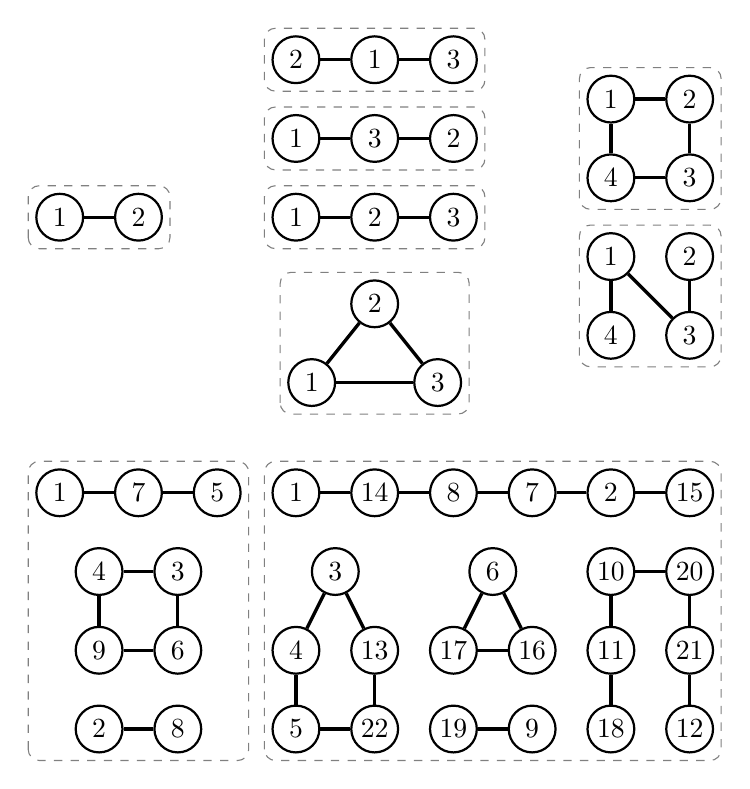
\begin{tikzpicture}
        \begin{scope}[every node/.style={circle,thick,draw,inner sep=0pt, text width=5.5mm, align=center}]
            \node (A1) at (-10,0) {1};
            \node (A2) at (-9,0) {2};

            \node (B1) at (-7, 0) {1};
            \node (B2) at (-6, 0) {2};
            \node (B3) at (-5, 0) {3};

            \node (C1) at (-7, 1) {1};
            \node (C2) at (-6, 1) {3};
            \node (C3) at (-5, 1) {2};

            \node (D1) at (-7, 2) {2};
            \node (D2) at (-6, 2) {1};
            \node (D3) at (-5, 2) {3};

            \node (E1) at (-6.8, -2.1) {1};
            \node (E2) at (-6, -1.1) {2};
            \node (E3) at (-5.2, -2.1) {3};

            \begin{scope}[shift={(0, -0.5)}]
            \node (F1) at (-3, 0) {1};
            \node (F2) at (-2, 0) {2};
            \node (F3) at (-2, -1) {3};
            \node (F4) at (-3, -1) {4};

            \node (G1) at (-3, 2) {1};
            \node (G2) at (-2, 2) {2};
            \node (G3) at (-2, 1) {3};
            \node (G4) at (-3, 1) {4};
            \end{scope}

            \begin{scope}[shift={(0,1.5)}]
            \node (H1) at (-10, -5) {1};
            \node (H7) at (-9, -5) {7};
            \node (H5) at (-8, -5) {5};
            \begin{scope}[shift={(0.5,0)}]
            \node (H4) at (-10, -6) {4};
            \node (H3) at (-9, -6) {3};
            \node (H6) at (-9, -7) {6};
            \node (H9) at (-10, -7) {9};
            \node (H2) at (-10, -8) {2};
            \node (H8) at (-9, -8) {8};
            \end{scope}
            \end{scope}

            \node (I1) at (-7, -3.5) {1};
            \node (I14) at (-6, -3.5) {14};
            \node (I8) at (-5, -3.5) {8};
            \node (I7) at (-4, -3.5) {7};
            \node (I2) at (-3, -3.5) {2};
            \node (I15) at (-2, -3.5) {15};
            
            \node (I3) at (-6.5, -4.5) {3};
            \node (I5) at (-7, -6.5) {5};
            \node (I4) at (-7, -5.5) {4};
            \node (I13) at (-6, -5.5) {13};
            \node (I22) at (-6, -6.5) {22};

            \node (I6) at (-4.5, -4.5) {6};
            \node (I17) at (-5, -5.5) {17};
            \node (I16) at (-4, -5.5) {16};

            \node (I19) at (-5, -6.5) {19};
            \node (I9) at (-4, -6.5) {9};

            \node (I10) at (-3, -4.5) {10};
            \node (I11) at (-3, -5.5) {11};
            \node (I18) at (-3, -6.5) {18};
            \node (I20) at (-2, -4.5) {20};
            \node (I21) at (-2, -5.5) {21};
            \node (I12) at (-2, -6.5) {12};
        \end{scope}

        \draw[rounded corners, draw=gray, dashed] (-10.4, -0.4) rectangle ++(1.8, 0.8);
        \draw[rounded corners, draw=gray, dashed] (-7.4, -0.4) rectangle ++(2.8, 0.8);
        \draw[rounded corners, draw=gray, dashed] (-7.4, 0.6) rectangle ++(2.8, 0.8);
        \draw[rounded corners, draw=gray, dashed] (-7.4, 1.6) rectangle ++(2.8, 0.8);
        \draw[rounded corners, draw=gray, dashed] (-7.2, -2.5) rectangle ++(2.4, 1.8);

        \draw[rounded corners, draw=gray, dashed] (-3.4, -1.9) rectangle ++(1.8, 1.8);
        \draw[rounded corners, draw=gray, dashed] (-3.4, 0.1) rectangle ++(1.8, 1.8);

        \draw[rounded corners, draw=gray, dashed] (-10.4, -6.9) rectangle ++(2.8, 3.8);

        \draw[rounded corners, draw=gray, dashed] (-7.4, -6.9) rectangle ++(5.8, 3.8);

        \begin{scope}[every edge/.style={draw=black, very thick}]
            \path [-] (A1) edge (A2);
            \path [-] (B1) edge (B2);
            \path [-] (C1) edge (C2);
            \path [-] (D1) edge (D2);
            \path [-] (E1) edge (E2);
            \path [-] (B2) edge (B3);
            \path [-] (C2) edge (C3);
            \path [-] (D2) edge (D3);
            \path [-] (E2) edge (E3);
            \path [-] (E1) edge (E3);
            \path [-] (F1) edge (F3);
            \path [-] (F1) edge (F4);
            \path [-] (F3) edge (F2);
            \path [-] (G1) edge (G2);
            \path [-] (G3) edge (G2);
            \path [-] (G3) edge (G4);
            \path [-] (G1) edge (G4);
            \path [-] (H1) edge (H7);
            \path [-] (H7) edge (H5);
            \path [-] (H4) edge (H3);
            \path [-] (H9) edge (H6);
            \path [-] (H9) edge (H4);
            \path [-] (H3) edge (H6);
            \path [-] (H2) edge (H8);

            \path [-] (I1) edge (I14);
            \path [-] (I14) edge (I8);
            \path [-] (I8) edge (I7);
            \path [-] (I7) edge (I2);
            \path [-] (I2) edge (I15);
            \path [-] (I3) edge (I4);
            \path [-] (I3) edge (I13);
            \path [-] (I4) edge (I5);
            \path [-] (I5) edge (I22);
            \path [-] (I22) edge (I13);
            \path [-] (I6) edge (I17);
            \path [-] (I6) edge (I16);
            \path [-] (I17) edge (I16);
            \path [-] (I19) edge (I9);
            \path [-] (I10) edge (I20);
            \path [-] (I10) edge (I11);
            \path [-] (I11) edge (I18);
            \path [-] (I20) edge (I21);
            \path [-] (I21) edge (I12);
        \end{scope}
    \end{tikzpicture}
    \caption{Some of the involved graphs in Exercise \ref{ex:3-7}}
    \label{fig:3:7}
    \end{figure}
\end{solution}

\begin{exercise}
    \label{ex:3-8}
    From 
    \[
        \sum_k \stirlingFst{n}{k} y^k = \coeff{\frac{x^n}{n!}}(1-x)^{-y} = n! \binom{y+n-1}{n} = y(y+1)\cdots (y+n-1)
    \] find a three term recurrence relation that is satisfied by the Stirling numbers of the first kind. Give a direct combinatorial proof of this recurrence relation. That is, reprove it, without using any generating functions.
\end{exercise}
\begin{solution}
    Note that:
    \[
        y(y+1)\cdots (y+n-1) = y(y+1)\cdots(y+n-2)y + y(y+1)\cdots (y+n-2)(n-1)  
    \]
    by the distributive property (split $y+n-1$ as $y + (n-1)$). Taking the coefficient corresponding to $y^k$ of each side gives:
    \[
        \stirlingFst{n}{k} = \coeff{y^k} \left(\bsum[k] \stirlingFst{n-1}{k}y^{k+1} + \stirlingFst{n-1}{k}y^k(n-1)\right) = \stirlingFst{n-1}{k-1} + (n-1)\stirlingFst{n-1}{k}
    \]
    For a combinatorial proof, we consider the cycle in which $n$ occurs. If it is a singleton cycle, there are $\stirlingFst{n-1}{k-1}$ configurations of the other elements. Otherwise, it occurs in one of the $k$ existing cycles. There are $(n-1)$ possibilities for the location (immediately following any of the other values) and $\stirlingFst{n-1}{k}$ configurations.
\end{solution}

\begin{exercise}
    Find the egf of the numbers $\{g(n)\}_0^\infty$ of permutations of $n$ letters that have both of the following properties: (a) they have an odd number of cycles and (b) the lengths of all of their cycles are even. Find a simple, explicit formula for these numbers.
\end{exercise}
\begin{solution}
    Take as cards the usual ones corresponding to cycles of permutations. The only decks with cards are the even-indexed ones with $d_{2n} = (2n-1)!$ such that the deck enumerator is
    \[
        \mathcal{D}(x) = \sum_{n = 1}^{\infty} (2n-1)!\frac{x^{2n}}{(2n)!} = \sum_{n = 1}^\infty \frac{x^{2n}}{2n} = \frac{1}{2} \sum_{n=1}^\infty \frac{(x^2)^n}{n} \estep{\eqref{eq:power_loggeom}} \frac{1}{2} \log \frac{1}{1-x^2}
    \]
    The hands enumerator follows from the exponential formula with number of cards restricted to an odd number using:
    \[
        e_T(x) = \bsum[t] \frac{x^{2t+1}}{(2t+1)!} \estep{\eqref{eq:power_sinh}} \sinh(x)
    \]
    The egf for the permutations that satisfies both properties is therefore:
    \begin{align*}
        \bsum g(n) \frac{x^n}{n!} &= \sinh\left(\log\frac{1}{\sqrt{1-x^2}}\right) = \frac{\frac{1}{\sqrt{1-x^2}} - \sqrt{1-x^2}}{2} = \frac{x^2}{2\sqrt{1-x^2}}
    \end{align*}
    To find a simple, explicit formula, we apply the binomial expansion:
    \begin{align*}
        g(n) &= \coeff{\frac{x^n}{n!}} \frac{x^2}{2\sqrt{1-x^2}} \\
        \estepalign{\eqref{eq:binom_num}} \coeff{\frac{x^n}{n!}} \frac{x^2}{2} \bsum[k] \binom{-\frac{1}{2}}{k}(-x^2)^k \\
        &= \coeff{\frac{x^n}{n!}}\frac{1}{2} \bsum[k] (-1)^k \binom{-\frac{1}{2}}{k} x^{2k + 2} \\
        &= \begin{cases}
            0 & \textnormal{if $n$ is odd} \\
            \frac{(-1)^{\frac{n}{2} - 1} n!}{2} \displaystyle\binom{-\frac{1}{2}}{\frac{n}{2} - 1} & \textnormal{if $n$ is even}
        \end{cases}
    \end{align*}
    Such that we can work with integer arithmetic on a computer, we rewrite the binomial such that the numerator is an integer. Let $n$ be even and $r = \frac{n}{2}$, then:
    \[
       g(n) = \frac{(-1)^{r - 1} n!}{2} \displaystyle\binom{-\frac{1}{2}}{r - 1}
    \]
    Using the generalized definition of the binomial:
    \[
        g(n) = \frac{(-1)^{r - 1} n!}{2(r-1)!}\left(-\frac{1}{2}\right)\left(-\frac{1}{2} - 1\right) \cdots \left(-\frac{1}{2}-r+2\right)
    \] 
    Factoring out $\frac{-1}{2}$ from each term:
    \[
        g(n) = \frac{(-1)^{r-1}n!}{2(r-1)!}\frac{(-1)^{r-1}}{2^{r-1}}(1)(1+2)\cdots(1+2r-4) = \frac{n!}{2^r(r-1)!}(1)(3)\cdots (n-3) 
    \]
    Multiplying and dividing by the even terms such that a factorial and subsequently a binomial coefficient can be recognized (also recall that $2r=n$):
    \begin{align*}
        g(n) &= \frac{n!}{2^r(r-1)!}(1)(3)\cdots(n-3) \frac{(2)(4)\cdots(n-2)}{(2)(4)\cdots(n-2)} \\
        &=  \frac{n!}{2^r(r-1)!} (n-2)! \frac{1}{2^{r-1}(1)(2)\cdots (r-1)} \\
       &= \frac{n!}{2^{n-1}} \binom{n-2}{r-1}
    \end{align*} 
\end{solution}

\begin{exercise}
    Find an explicit formula for $\stirlingSnd{n}{k}$, the Stirling numbers of the second kind by expanding the $k$th power that appears in 
    \[
        \stirlingSnd{n}{k} = \coeff{\frac{x^n}{n!}}\left\{\frac{(e^x-1)^k}{k!}\right\}
    \]
    by the binomial theorem. Your formula should be in the form of a single finite sum.
\end{exercise}
\begin{solution}
    Applying the binomial theorem gives:
    \begin{align*}
        \stirlingSnd{n}{k} &= \coeff{\frac{x^n}{n!}}\left\{\frac{(e^x-1)^k}{k!}\right\} \\
        \estepalign{\eqref{eq:binom_num}} \coeff{\frac{x^n}{n!}} \frac{1}{k!} \bsum[m] \binom{k}{m} e^{xm} (-1)^{k-m} \\
        &=  \bsum[m]\binom{k}{m} \frac{(-1)^{k-m}}{k!} \coeff{\frac{x^n}{n!}}e^{xm} \\
        &= \bsum[m] \binom{k}{m} \frac{(-1)^{k-m}m^n}{k!}
    \end{align*}
    Writing it as a finite sum by discarding the values for which the summand becomes $0$:
    \[
        \stirlingSnd{n}{k} = \sum_{m=0}^{k} \frac{(-1)^{k-m}m^n}{m!(k-m)!}
    \]
\end{solution}

\begin{exercise}
    Let $S$, $T$ be fixed sets of positive integers. Let $f(n;S,T)$ be the number of partitions of $[n]$ whose class sizes all lie in $S$ and whose number of classes lie in $T$. Show that $\{f(n;S,T)\}_{n\geq0}$ has the egf $e_T(e_S(x))$, where $e_S(x) = \sum_{s\in S} \frac{x^s}{s!}$.
\end{exercise}
\begin{solution}
    The cards are the usual ones for set partitions. Since every deck corresponding to a permittable class size has one card, the deck enumerator is:
    \[
        \mathcal{D}(x) = \sum_{s\in S} 1 \cdot \frac{x^s}{s!} = e_S(x)
    \]
    The exponential formula with restricted number of cards (number of classes), then immediately gives the asked answer:
    \[
        \bsum f(n;S,T) \frac{x^n}{n!} = e_T(e_S(x))
    \]
\end{solution}

\begin{exercise}
    Fix $k>0$. Let $f(n,k)$ be the number of permutations of $n$ letters whose longest cycle has length $k$. Find the egf of $\{f(n,k)\}_{n\geq0}$, for $k$ fixed.
\end{exercise}
\begin{solution}
    Let $g(n,k)$ be the number of permutations of $n$ letters whose cycles have lengths $\leq k$. Then the answer is given by $g(n,k) - g(n,k-1)$.

    As cards, we use the usual ones corresponding to cycles of permutations. Only cycle lengths $\leq k$ are allowed, so the deck enumerator is:
    \[
        \mathcal{D}(x) = \sum_{m=1}^k (m-1)! \frac{x^m}{m!} = \sum_{m=1}^k \frac{x^m}{m}
    \]
    Then, by the exponential formula:
    \[
        \bsum g(n,k) \frac{x^n}{n!} = \exp\left(\sum_{m=1}^k \frac{x^m}{m}\right)
    \]
    and:
    \begin{align*}
        \bsum f(n,k) \frac{x^n}{n!} &= \exp\left(\sum_{m=1}^k \frac{x^m}{m}\right) - \exp\left(\sum_{m=1}^{k-1} \frac{x^m}{m}\right) \\
        &= \exp\left(\sum_{m=1}^{k-1} \frac{x^m}{m}\right) \left(\exp\left(\frac{x^k}{k}\right) - 1\right)
    \end{align*}
\end{solution}

\begin{exercise}
    If $T(x)$ and $\mathcal{G}(x)$ denote, respectively, the egf's of involutions:
    \[
        T(x) = \sum_{n\geq 0}t_n\frac{x^n}{n!} = e^{x+\frac{1}{2}x^2}
    \]
    and of 2-regular graphs:
    \[
        \mathcal{G}(x) = \sum_{n\geq0}g(n) \frac{x^n}{n!}  = \frac{e^{-\frac{1}{2}x-\frac{1}{4}x^2}}{\sqrt{1-x}}
    \]
    then observe that:
    \[
        T(x)\mathcal{G}(x)^2 = \frac{1}{1-x}
    \]
    \begin{enumerate}[label=(\alph*)]
        \item Write out the identity between the sequences $\{g(n)\}$ and $\{t(n)\}$ that is implied by the above generating function relation.
        \item Show that for each fixed $n\geq1$ there are exactly the same numbers of
        \begin{enumerate}[label=(\roman*)]
            \item permutations of $n$ letters and of
            \item triples $(\tau,G_1,G_2)$, where $\tau$ is an involution of a set $R$, $G_1$ is a $2$-regular graph on a vertex set $S$, $G_2$ is a $2$-regular graph on a vertex set $T$, and $R$, $S$, $T$ partition $[n]$.
        \end{enumerate}
        \item Find, explicitly, a 1-1 correspondence such as is described in part (b) above.
    \end{enumerate}
\end{exercise}
\begin{solution}
    \begin{enumerate}[label=(\alph*)]
        \item Equating coefficients of $\frac{x^n}{n!}$ on both sides gives:
        \[
            \coeff{\frac{x^n}{n!}}\sum_{r,s,t \geq 0} t_r \frac{x^r}{r!} g_s \frac{x^s}{s!} g_t\frac{x^t}{t!} = \coeff{\frac{x^n}{n!}} \sum_{k\geq 0} x^k \Longleftrightarrow \sum_{r+s+t=n} \frac{n!}{r!s!t!}t_rg_sg_t = n!
        \]
        \item The multinomial coefficient gives the number of ways of partitioning $[n]$ into three parts, with $r$ numbers in the first part, $s$ in the second part and $t$ in the third part. $t_r$ counts the number of involutions which gets relabeled by the numbers in that class $R$. Similarly, $g_s$ and $g_t$ count the number of $2$-regular graphs relabeled using their respective classes.
        
        Adding these over all possible class sizes which sum to $n$ gives the left side. The number of permutations is on the right side.
        \item We give a construction from a triplet $(\tau, G_1, G_2)$ to a permutation $\sigma$. All involutions of $\tau$ will be mapped to the same cycles in $\sigma$. This will be one-to-one since $2$-regular graphs with cycle lengths of $2$ or less are impossible. Therefore from a permutation $\sigma$, its fixed points and length $2$-cycles in its cycle decomposition are in unique correspondence with $\tau$.
        
        Now for each cycle in $G_1$, we start from its smallest element (it doesn't matter from where a cycle in a permutation starts due to cyclic invariance) and map the cycle in the graph to a cycle in $\sigma$. There are $2$ ways to traverse the cycle in the graph. Let $G_1$ always go in the direction of the smallest element and $G_2$ in the direction of the largest element. Note that this construction is uniquely invertible since for every cycle in $\sigma$, we check the second element and the last element for which one is the largest which fixes the choice of $G_1$ and $G_2$ and the cycle in the corresponding graph.
    \end{enumerate}
\end{solution}

\begin{exercise}
    Let $\mathcal{F}$ be an exponential family with associated polynomials $\{\phi_n(x)\}$ of binomial type and with deck enumerator $\mathcal{D}(x)$.
    \begin{enumerate}[label=(\alph*)]
        \item If $D_y$ denotes the differential operator $\partial/\partial y$, then show that
        \[
            \mathcal{D}^{(-1)}(D_y)\phi_n(y) = n\phi_{n-1}(y) \quad (n\geq 0)
        \]
        by directly applying the operator to the egf of the polynomial sequence (here $\mathcal{D}^{-1}$ denotes the inverse function in the sense of functional composition).
        \item In the case of the exponential family of permutations by cycles, find the associated polynomials of binomial type, and verify the identity proved in part (a) by direct computation with those polynomials.
    \end{enumerate}
\end{exercise}
\begin{solution}
    \begin{enumerate}[label=(\alph*)]
        \item The polynomials of binomial type satisfy the generating relation:
        \[
            e^{y\mathcal{D}(x)} = \bsum \phi_n(y)\frac{x^n}{n!}
        \]
        Applying $D_y$ to the left side adds a factor of $\mathcal{D}(x)$ to the front. Applying a function $f(D_y)$ is therefore equivalent to multiplying by $f(\mathcal{D}(x))$. Choosing $f$ to be $\mathcal{D}^{-1}$ therefore multiplies the left side by $\mathcal{D}^{(-1)}(\mathcal{D}(x)) = x$. We now find:
        \[
            \mathcal{D}^{(-1)}(D_y) \bsum \phi_n(y) \frac{x^n}{n!} = x\bsum \phi_n(y) \frac{x^n}{n!} = \sum_{n=1}^\infty \phi_{n-1}(y)\frac{x^n}{(n-1)!}
        \]
        Equating coefficients of $\frac{x^n}{n!}$ gives the desired relation.
        \item The deck enumerator of permutations by cycles is:
        \[
            \mathcal{D}(x) = \log\frac{1}{1-x} \quad \textnormal{with inverse} \quad  \mathcal{D}^{(-1)}(x) = 1-e^{-x}
        \]
        The associated polynomials of binomial type are found from:
        \[
            e^{y\mathcal{D}(x)} = \frac{1}{(1-x)^y} \estep{\eqref{eq:binom_num}} \bsum \binom{-y}{n}(-x)^n = \bsum y(y+1)\cdots (y+n-1) \frac{x^n}{n!}
        \]
        \[
            \implies \phi_n(y) = y(y+1)\cdots (y+n-1)
        \]
        Now, the left-hand side of the relation is:
        \[
            \mathcal{D}^{(-1)}(D_y)\phi_n(y) = \phi_n(y) - e^{-D_y}\phi_n(y) = \phi_n(y) - \bsum[k] \frac{(-1)^k D_y^k}{k!}\phi_n(y) 
        \]
        We can write this last term in a more suggestive form
        \[
            \mathcal{D}^{(-1)}(D_y)\phi_n(y) = \phi_n(y) - \bsum[k] \frac{((y-1) - y)^k}{k!} D_y^k\phi_n(y)
        \]
        The sum is $\phi_n(y-1)$ from Taylor's theorem. We therefore have:
        \[
            \mathcal{D}^{(-1)}(D_y)\phi_n(y) = \phi_n(y) - \phi_n(y-1)
        \]
        Plugging in the polynomials:
        \begin{align*}
            \mathcal{D}^{(-1)}(D_y)\phi_n(y) &= y(y+1)\cdots (y+n-1) - (y-1)y\cdots (y+n-2) \\
            &= y(y+1)\cdots(y+n-2)\big\{y+n-1 - (y-1)\big\} \\
            &= y(y+1)\cdots (y+n-2)n \\
            &= n\phi_{n-1}(y)
        \end{align*}
        which is indeed what we were after.
    \end{enumerate}
\end{solution}

\begin{exercise}
    In an exponential family $\mathcal{F}$, let $\tilde{h}(n)$ be the number of hands of weight $n$ whose cards have all different weights.
    \begin{enumerate}[label=(\alph*)]
        \item Show that
        \[
            \sum_{n\geq0} \tilde{h}(n) \frac{x^n}{n!} = \prod_{k=1}^\infty \left\{1+d_k\frac{x^k}{k!}\right\}
        \]
        \item Let $p_n$ be the probability that a permutation of $n$ letters has cycles whose lengths are all different. Then show that
        \[
            \{p_n\}\stackrel{ops}{\longleftrightarrow} \prod_{k\geq 1}\left\{1+\frac{x^k}{k}\right\}
        \]
        \item If $p(x)$ denotes the generating function in part (b) above, determine the growth of $p(x)$ as $x\to 1^-$. Do this by inserting additional factors of $e^{-x^k/k}$ in the product.
    \end{enumerate}
\end{exercise}
\begin{solution}
    \begin{enumerate}[label=(\alph*)]
        \item We first show that the statement is true for an exponential family with only one nonempty deck and then the result follows from the fundamental lemma of labeled counting.
        
        Consider the exponential family $\mathcal{F}_k$ where the $k$th deck is the only nonempty one with $d_k$ cards. Then the hand enumerator which satisfy the condition is given by: 
        \[
            \mathcal{H}(x) = 1 + d_k \frac{x^k}{k!}
        \]
        since there is one hand with weight $0$ (the empty hand) and $d_k$ hands with weight $k$. Other hands are not possible since we can't take multiple cards of the same weight.

        We can now apply the same proof from the fundamental lemma of labeled counting to the merger of all families $\mathcal{F}_k$ to show that:
        \[
            \tilde{\mathcal{H}}(x) = \prod_{k=1}^\infty \left\{1+d_k \frac{x^k}{k!}\right\}
        \]
        Note that the same proof can be used since the hand enumerator of the merger of two families who have no cards of the same weight in common will have hands with cards with all different weights (as long as the hand enumerators of the families satisfy the same condition).
        \item Let $\tilde{h}(n)$ denote the number of permutations of $n$ letters whose cycles are all different lengths. Because $d_k = (k-1)!$ for cycles of permutations, we immediately find:
        \[
            \bsum p_n x^n = \bsum \frac{\tilde{h}(n)}{n!} x^n = \prod_{k=1}^\infty \left\{ 1 + (k-1)!\frac{x^k}{k!}\right\} = \prod_{k=1}^\infty \left\{ 1 + \frac{x^k}{k}\right\}
        \]
        \item Inserting additional factors of $e^{-x^k/k}$ into the product gives:
        \begin{align*}
            \prod_{k=1}^\infty \left\{1+\frac{x^k}{k}\right\} &= \prod_{k'=1}^\infty e^{x^{k'}/k'} \prod_{k=1}^\infty \left(1+ \frac{x^k}{k} \right) e^{-x^k/k} \\
            &= \exp\left(\sum_{k'=1}^\infty \frac{x^{k'}}{k'}\right)\prod_{k=1}^\infty \left(1+ \frac{x^k}{k} \right) e^{-x^k/k} \\
            \estepalign{\eqref{eq:power_loggeom}} \exp\left(\log\frac{1}{1-x}\right)\prod_{k=1}^\infty \left(1+ \frac{x^k}{k} \right) e^{-x^k/k} \\
            &= \frac{1}{1-x}\prod_{k=1}^\infty \left(1+ \frac{x^k}{k} \right) e^{-x^k/k}
        \end{align*}
        For $x \to 1^-$, the infinite product approaches a constant. Indeed, taking the logarithm gives:
        \[
            \log\left(\prod_{k=1}^\infty \left(1+ \frac{1}{k} \right) e^{-1/k}\right) = \sum_{k=1}^\infty \frac{-1}{k} + \log\left(1+\frac{1}{k}\right) = -\gamma
        \]
        where $\gamma$ is the Euler--Mascheroni constant. We therefore have:
        \[
            p(x) \sim \frac{e^{-\gamma}}{1-x}
        \]
        as $x\to 1^-$.
    \end{enumerate}
\end{solution}

\begin{exercise}
    Let numbers $\{c_n\}$ be defined by
    \[
        x^x = 1 + \sum_{n\geq 1}\frac{c_n}{n!}(x-1)^n
    \]
    Show that each $c_n$ is an integer multiple of $n$, and in fact is a multiple of $n(n-1)$ if and only if $n-1$ divides $(n-2)!$.
\end{exercise}
\begin{solution}
    Substituting $x \to x+1$, we see that:
    \[
        (x+1)^{x+1} = 1 + \sum_{n=1}^\infty c_n \frac{x^n}{n!} 
    \]
    such that $c_n$ is the coefficient of $\frac{x^n}{n!}$ in $(x+1)^{x+1}$. Now applying the binomial theorem:
    \begin{align*}
        (x+1)^{x+1} &= (x+1)(x+1)^x \\
        \estepalign{\eqref{eq:binom_num}} (x+1)\bsum[k] \binom{x}{k}x^k \\
        &= (x+1) \bsum[k] \frac{x(x-1)\cdots (x-k+1)}{k!}x^k \\
        &= (x+1) \bsum[k] (-1)^k \frac{(-x)(-x+1)\cdots(-x+k-1)}{k!}x^k
    \end{align*}
    From the opsgf of the Stirling numbers of the first kind, we then have:
    \[
        (x+1)^{x+1} = (x+1) \bsum[k] (-1)^k \frac{x^k}{k!} \bsum[m] \stirlingFst{k}{m} (-x)^m
    \]
    such that $c_n$ is:
    \begin{align*}
        c_n &= \coeff{\frac{x^n}{n!}}(x+1) \bsum[k] (-1)^k \frac{x^k}{k!} \bsum[m]\stirlingFst{k}{m} (-x)^m \\
        &= \coeff{\expcoeff} \left\{\bsum[k] \bsum[m] (-1)^{k+m} \frac{x^{m+k+1}}{k!} \stirlingFst{k}{m} + (-1)^{k+m} \frac{x^{m+k}}{k!} \stirlingFst{k}{m}\right\} \\
        &= n!\bsum[l]  \frac{(-1)^{n-1}}{l!} \stirlingFst{l}{n-l-1} + \frac{(-1)^n}{l!}\stirlingFst{l}{n-l}
    \end{align*}
    Because $\stirlingFst{n}{k}$ is zero when $k\leq 0$ or in this case $l\geq n$, we have that the right side definitely contains a factor of $n$ (from the factorial and due to the fact that $l < n$ thereby not dividing away the factor of $n$). 
    
    Furthermore, for $l = n-1$, the first term in the sum becomes $0$ by the same argument and the second is $(-1)^n \frac{(n-2)!}{(n-1)!}$, after multiplying with $n!$, it is divisible by $n(n-1)$ if and only if $n$ divides $(n-2)!$. The other terms are all divisible by $n(n-1)$ because $l < n-1$.
\end{solution}

\begin{exercise}
    Here we want to show that the Stirling numbers of the first and second kinds are inverse to each other, in a certain sense. In the generating function
    \[
        \sum_k \stirlingFst{n}{k}x^k = x(x+1)\cdots (x+n-1)
    \]
    for the former, replace $x$ by $\frac{-1}{x}$ and compare with the generating function 
    \[
        \sum_n \stirlingSnd{n}{k}x^n = \frac{x^k}{(1-x)(1-2x)\cdots (1-kx)}
    \]
    for the latter. Multiply the functions together so that the hard part cancels out. Read off the coefficient of $x^0$ in what remains, and state it as an assertion that a certain pairs of matrices, each involving Stirling numbers, are inverses of each other.
\end{exercise}
\begin{solution}
    Replacing $x$ by $\frac{-1}{x}$ gives:
    \[
        \bsum[m] \stirlingFst{n}{m}\frac{(-1)^m}{x^m} = \frac{1(1-x)(1-2x)\cdots (1-x(n-1))}{(-1)^nx^n}
    \]
    Multiplying by:
    \[
        \bsum[l] \stirlingSnd{l}{k}x^l = \frac{x^k}{(1-x)(1-2x)\cdots(1-kx)}
    \]
    gives:
    \[
        \bsum[m] \bsum[l] \stirlingFst{n}{m} \stirlingSnd{l}{k} (-1)^m x^{l-m} = \frac{(-1)^n x^{k-n}(1-x)\cdots(1-x(n-1))}{(1-x)(1-2x)\cdots(1-kx)}
    \]
    Looking at the constant coefficient, we find:
    \begin{align*}
        \bsum[m] \stirlingFst{n}{m}\stirlingSnd{m}{k}(-1)^m &= \begin{cases}
            \coeff{x^0} (-1)^n x^{k-n} \prod_{r=k+1}^{n-1} (1-xr) = 0, & k < n \\
            \coeff{x^0} (-1)^n \frac{1}{1-kx} \estep{\eqref{eq:power_geom}} (-1)^n, & k = n \\
            \coeff{x^0} (-1)^n x^{k-n} \prod_{r=n}^k \frac{1}{1-rx} = 0, & k > n
        \end{cases}
    \end{align*}
    where the first case follows from the fact that all powers of $x$ will be strictly negative and the last case follows from the fact that all powers of $x$ will be strictly positive. We therefore have the identity:
    \[
        \bsum[m] \stirlingFst{n}{m}\stirlingSnd{m}{k}(-1)^{m}(-1)^n = \delta_{kn}
    \]
    In matrix notation, this becomes:
    \[
        S_1 S_2 = I
    \]
    where:
    \[
        (S_1)_{ij} = (-1)^{j-i}\displaystyle\stirlingFst{i}{j}, \quad (S_2)_{ij} = \displaystyle\stirlingSnd{i}{j}
    \]
\end{solution}

\begin{exercise}
    Let $a_n$ be the number of \emph{unlabeled} graphs of $n$ vertices each of whose connected components is a path or a cycle. Let $F(x)$ be the opsgf of the sequence $\{a_n\}$. Find $F(x)$ and express it in terms of Euler's opsgf for the sequence $\{p(n)\}$ of the numbers of partitions of integers $n$.
\end{exercise}
\begin{solution}
    The cards are the usual ones corresponding to connected components, but they are now unlabeled. The deck sizes are:
    \[
        d_n = \begin{cases}
            1 & 1 \leq n \leq 2 \\
            2 & n \geq 3
        \end{cases}
    \]
    since there is only unlabeled path for $n \geq 1$ and one unlabeled cycle for $n \geq 3$. Recall that in a prefab, we have the identity
    \[
        \mathcal{H}(x) = \prod_{r=1}^\infty \frac{1}{(1-x^r)^{d_r}}
    \]
    where $\mathcal{H}(x)$ is the hand enumerator. In our case, we have that
    \[
        F(x) = \frac{1}{1-x} \frac{1}{1-x^2} \prod_{r=3}^\infty \frac{1}{(1-x^r)^2}
    \]
    Recall that the opsgf for the sequence of number of partitions of integers $n$ is given by:
    \[
        P(x) = \prod_{r=1}^\infty \frac{1}{1-x^r}
    \]
    such that:
    \[
        F(x) = (1-x)(1-x^2)P(x)^2
    \]
\end{solution}

\begin{exercise}
    Let $a_n$ be the number of unlabeled rooted trees of $n$ vertices in which the degree of the root is $2$. That is, there are exactly $2$ edges incident at the root. Let $T(x)$ be the opsgf of the sequence $\{t_n\}$ that counts \emph{all} rooted trees of $n$ vertices. Show that:
    \[
        \sum_n a_nx^{n-1} = \frac{1}{2}\left(T(x)^2 + T(x^2)\right)
    \]
\end{exercise}
\begin{solution}
    An unlabeled rooted tree of $n$ vertices where the degree of the root is $2$ corresponds to an unordered pair of rooted trees whose size sum up to $n-1$. If $(n-1)$ is odd, this is:
    \[
        a_n = \frac{1}{2} \bsum[j] t_j t_{n-1-j}
    \]
    We divide by $2$ since the pairs are unordered.
    
    If $(n-1)$ is even, the two subtrees may be the same size. When they are the same size, there are $\frac{1}{2}t_{(n-1)/2}^2 + \frac{1}{2}t_{(n-1)/2}$ unordered pairs to compensate for the fact thate these pairs were subtracted twice. This adds an additional term $\frac{1}{2}t_{(n-2)/2}$ to the above expression for $n$ odd. We therefore have:
    \[
        \sum_{n=1}^\infty a_nx^{n-1} = \left\{\bsum[n] \frac{1}{2} \bsum[j] t_j t_{n-1-j}x^{n-1}\right\} + \bsum[k]\frac{1}{2}t_kx^{2k} = \frac{1}{2}\left(T(x)^2 + T(x^2)\right)
    \]
\end{solution}

\begin{exercise}
    Find the largest integer that is \emph{not} of the form $6x+10y+15z$ where $x,y,z$ are nonnegative integers. \emph{Prove} that your answer is correct, i.e., that your integer is not so representable, and that every integer larger than it is so representable.
\end{exercise}
\begin{solution}
    Note that $29$ can't be represented in that form since it is clearly not of the form:
    \[
        6x + 10y + 15\cdot 0 \quad \textnormal{or} \quad 6x+10y+15\cdot 1
    \]
    Now, observe that following integers are representable:
    \begin{align*}
        30 &= 6\cdot 0 + 10\cdot 3 + 15\cdot 0 \\
        31 &= 6\cdot 1 + 10\cdot 1 + 15\cdot 1 \\
        32 &= 6 \cdot 2 + 10\cdot 2 + 15\cdot 0 \\
        33 &= 6\cdot 3 + 10\cdot 0 + 15\cdot 1 \\
        34 &= 6\cdot 4 + 10 \cdot 1 + 15\cdot 1 \\
        35 &= 6\cdot 0 + 10\cdot 2 + 15 \cdot 1
    \end{align*}
    and note that if $n$ is representable, so is $n+6$ (by incrementing $x$) and therefore all integers larger than $29$ are representable.
\end{solution}

\begin{exercise}
    In a country that has $1$-cent, $2$-cent, and $3$-cent coins only, show that the number of ways of changing $n$ cents is exactly the integer \emph{nearest} to $(n+3)^2/12$.
\end{exercise}
\begin{solution}
    Let $h(n)$ denote the number of ways of changing $n$ cents. Then its opsgf is given by:
    \[
        \mathcal{H}(x) = \frac{1}{(1-x)(1-x^2)(1-x^3)}  
    \]
    Factoring the denominator gives:
    \begin{align*}
        \mathcal{H}(x) &= \frac{1}{(1-x)(1-x^2)(1-x^3)} \\
        &= \frac{1}{(1-x)(1-x)(1+x)(1-x)(1-\omega_+ x)(1-\omega_-x)}
    \end{align*}
    where $\omega_{\pm} = e^{\frac{\pm2\pi i}{3}}$. Partial fraction decomposition now gives:
    \begin{align*}
        \mathcal{H}(x) &= \frac{A}{(1-x)^3} + \frac{B}{(1-x)^2} + \frac{C}{1-x} + \frac{D}{1+x} + \frac{E}{1-\omega_+x} + \frac{F}{1-\omega_-x}
    \end{align*}
    $A$, $D$, $E$, $F$ are easily found:
    \begin{alignat*}{4}
        A &= \lim_{x\to 1}(1-x)^3\mathcal{H}(x) = \frac{1}{6} &&&\qquad D &= \lim_{x\to -1}(1+x)\mathcal{H}(x) = \frac{1}{8} \\
        E &= \lim_{x\to \omega_-}(1-\omega_+x)\mathcal{H}(x) = \frac{1}{9} &&&\qquad  F &= \lim_{x\to\omega_+}(1-\omega_-x)\mathcal{H}(x) = \frac{1}{9}
    \end{alignat*}
    To find $B$, multiply both sides by $(1-x)^3$, differentiate and let $x\to 1$ to get:
    \[
        \frac{-1}{4} = -B \Leftrightarrow B = \frac{1}{4}
    \]
    To find $C$ evaluate both sides at $0$:
    \[
        1 = A + B + C + D + E + F \Leftrightarrow C = \frac{17}{72}
    \]
    Now, writing as a power series (utilizing \eqref{eq:binom_denom}, \hyperlink{eq:ch1:1:a}{1.1(a)}, \eqref{eq:power_geom}):
    \[
        \mathcal{H}(x) = \bsum[m] \left(A\binom{m+2}{2} + B(m+1) + C + D(-1)^m + E\omega_+^m + F\omega_-^m\right)x^m
    \]
    And extracting the coefficient of $x^n$:
    \begin{align*}
        h(n) &= A\binom{n+2}{2}+B(n+1)+C+D(-1)^n + 2E\cos\left(\frac{2\pi n}{3}\right) \\
        &= \frac{n^2+3n+2}{12} +  \frac{n+1}{4} + \frac{17}{72} + \frac{(-1)^n}{8} + \frac{2}{9}\cos\left(\frac{2\pi n}{3}\right) \\
        &= \frac{(n+3)^2}{12} + \frac{-7 + 9(-1)^n + 16\cos\left(\frac{2\pi n}{3}\right)}{72}
    \end{align*}
    The right part is always smaller than $\frac{7+9+16}{72} = \frac{32}{72} < \frac{1}{2}$ in absolute value, therefore $h(n)$ is exactly the nearest integer to $\frac{(n+3)^2}{12}$.
\end{solution}

\begin{exercise}
    This exercise develops a considerable sharpening of the exponential formula.
    \begin{enumerate}[label=(\alph*)]
        \item In an exponential family $\mathcal{F}$, the number of hands of weight $n$ that contain exactly $a_1$ cards of weight $1$ and $a_2$ cards of weight $2$ and $a_3$ of weight $3$ and \ldots, where $a_1+2a_2+\ldots  = n$, is the coefficient of $(t^nx_1^{a_1}x_2^{a_2}\cdots)/n!$ in the expansion of 
        \[
            \exp\left\{\sum_{i\geq 1} \frac{x_id_it^i}{i!}\right\}
        \]
        \item Let $f(n,r,s)$ be the number of partitions of the set $[n]$ that have exactly $r$ classes of size $1$ and exactly $s$ classes of size $2$ (however many classes of other sizes they may have). Then
        \[
            \sum_{n,r,s}f(n,r,s)x^ry^s\frac{t^n}{n!} = \exp\left(xt+\frac{yt^2}{2}+e^t -1-t-\frac{t^2}{2}\right)
        \]
    \end{enumerate}
\end{exercise}
\begin{solution}
    \begin{enumerate}[label=(\alph*)]
        \item \hypertarget{eq:ch3:22:a}{} By reasoning similar to Exercise \ref{ex:2-21}, one can view $x_i$ as counting the number of times $d_i$ is taken and then the result immediately follows from the exponential formula.
        
        For a more rigorous argument, we enumerate all hands of weight $n$ that satisfy $a_1 + 2a_2 + \ldots = n$. First, choose all the cards in a hand, there are $d_1^{a_1}d_2^{a_2}\cdots$ way to do this. For the cards of weight $1$, choose its labels. There are $\binom{n}{a_1}$ ways to do this. Then, for the cards with weight $2$, there are:
        \[
            \binom{n-a_1}{2} \binom{n-a_1-2}{2}\cdots \binom{n-a_1-2a_2 + 2}{2} = \frac{(n-a_1)!}{(n-a_1-2a_2)!(2!)^{a_2}}
        \]
        ways to do this. However, since the order of the cards in the hand does not matter, we have overcounted by $a_2!$ times, so the number of ways to choose the labels in an unordered way is:
        \[
           \frac{(n-a_1)!}{(n-a_1-2a_2)!(2!)^{a_2}a_2!}
        \]
        Similarly, for the cards with weight $k$, there are
        \[
            \frac{(n-a_1-2a_2-\cdots - (k-1)a_{k-1})!}{(n-a_1-2a_2-\cdots - ka_k)! (k!)^{a_k}a_k!}
        \]
        ways to choose their labels in an unordered way. Multiplying all these quantities gives:
        \[
            \frac{n!}{(1!)^{a_1}(2!)^{a_2}(3!)^{a_3}\cdots a_1!a_2!a_3!\cdots}d_1^{a_1}d_2^{a_2}d_3^{a_3}\cdots
        \]
        This is indeed the coefficient of the expansion of the given expression:
        \[
            \coeff{\frac{t^nx_1^{a_1}\cdots}{n!}} \exp\left\{\sum_{i=1}^\infty \frac{x_id_it^i}{i!}\right\} \estep{\eqref{eq:power_exp}} \coeff{\frac{t^nx_1^{a_1}\cdots}{n!}} \bsum[k] \frac{\left(\sum_{i=1}^\infty\frac{x_id_it^i}{i!}\right)^k}{k!}
        \]
        Define $f(t)$ to be the egf of $\{x_i d_i\}_{i= 1}^\infty$:
        \begin{align*}
            \coeff{\frac{t^nx_1^{a_1}\cdots}{n!}}  \exp\left\{\sum_{i=1}^\infty \frac{x_id_it^i}{i!}\right\} &= \coeff{\frac{t^nx_1^{a_1}\cdots}{n!}}  \bsum[k] \frac{f(t)^k}{k!} \\
            &= \coeff{x_1^{a_1}\ldots}\bsum[k] \frac{\coeff{\frac{t^n}{n!}} f(t)^k}{k!} \\
            &= \coeff{x_1^{a_1}\ldots}\bsum[k] \frac{\sum_{b_1+\ldots + b_k = n} n! \prod_{i=1}^{k} \frac{x_{b_i}d_{b_i}}{b_i!}}{k!} \\
            &= \coeff{x_1^{a_1}\ldots}\bsum[k] \sum_{b_1+\ldots + b_k = n} \frac{n!}{k!} \prod_{i=1}^{k} \frac{x_{b_i}d_{b_i}}{b_i!}
        \end{align*}
        Now, what is the coefficient corresponding to $x_1^{a_1}x_2^{a_2}\ldots$? For sure, it is accompanied by a factor of the form
        \[
            n!\frac{d_1^{a_1}d_2^{a_2}\cdots}{(1!)^{a_1}(2!)^{a_2}\cdots}
        \]
        where the $n!$ comes from the term in front and the $\frac{d_i^{a_i}}{(i!)^{a_i}}$ follow from the fact that we require that $i$ is present $a_i$ times in the (multi)set $\{b_1, b_2, \ldots\}$ (note that the constraint $a_1+2a_2+\cdots=n$ is then indeed satisfied). However, note that there are multiple ways to obtain such an arrangement. In particular, any permutation of the multiset $\{\underbrace{1, \ldots, 1}_{a_1 \textnormal{ times}}, \underbrace{2, \ldots, 2}_{a_2 \textnormal{ times}}, \ldots\}$ yields such a factor. The number of permutations of this multiset is given by the multinomial coefficient
        \[
            \binom{a_1 + a_2 + \cdots}{a_1!a_2!\cdots}.
        \]
        To conclude we have that
        \begin{align*}
            \coeff{\frac{t^nx_1^{a_1}\cdots}{n!}} \exp\left\{\sum_{i=1}^\infty \frac{x_id_it^i}{i!}\right\}  &= \frac{n!}{(a_1+\cdots)!} \frac{(a_1+\cdots)!}{a_1!a_2!\cdots}\frac{d_1^{a_1}d_2^{a_2} \cdots}{(1!)^{a_1}(2!)^{a_2}\cdots } \\
            &= \frac{n!d_1^{a_1}d_2^{a_2}\cdots}{(1!)^{a_1}(2!)^{a_2}\cdots a_1!a_2!}
        \end{align*}
        which matches the required value.
        \item There is one card in every deck size in the exponential family of set partitions. Applying the previous formula with $x_i = 1$ for $i \geq 3$ gives:
        \begin{align*}
            \sum_{n,r,s}f(n,r,s)x^ry^s\frac{t^n}{n!} &= \exp\left\{xt + \frac{yt^2}{2!} + \sum_{i=3}^\infty\frac{t^i}{i!}\right\} \\
            \estepalign{\eqref{eq:power_exp}} \exp\left\{xt + \frac{yt^2}{2} + e^t - 1 - t - \frac{t^2}{2}\right\}
        \end{align*}
    \end{enumerate}
\end{solution} \newpage
    \section{Applications of Generating Functions}
\begin{exercise}
    Given a coin whose probability of turning up `heads' is $p$, let $p_n$ be the probability that the first occurrence of `heads' is at the $n$th toss of the coin. Evaluate $p_n$ and the opsgf of the sequence $\{p_n\}$. Use that opsgf to find the mean of the number of trials till the first `heads' and the standard deviation of that number.
\end{exercise}
\begin{solution}
    Clearly, $p_n = (1-p)^{n-1}p$ ($n-1$ times tails and then heads) with opsgf:
    \[
        P(x) = \sum_{n= 1}^\infty p_n x^n= \sum_{n=1}^\infty (1-p)^{n-1}p x^n = px \bsum (1-p)^n x^n \estep{\eqref{eq:power_geom}} \frac{px}{1-(1-p)x}
    \]
    The mean number of trials is given by 
    \[\mu = P'(1) = \left\{\frac{p(1-(1-p)x) + (1-p)px}{(1-(1-p)x)^2}\right\}_{x=1} = \frac{1}{p}\] and the variance by:
    \begin{align*}
        \sigma^2 &= \{(\log P)' + (\log P)''\}_{x=1} \\
        &= \left\{\frac{1}{px^2-x^2 + x} + \frac{-2(p-1)x-1}{x^2((p-1)x+1)^2}\right\}_{x=1} \\
        &= \frac{1-p}{p^2}
    \end{align*}
\end{solution}

\begin{exercise}
    In the \emph{coupon collector's problem} we imagine that we would like to get a complete collection of photos of movie stars, where each time we buy a box of cereal we acquire one such photo, which may of course duplicate one that is already in our collection. Suppose there are $d$ different photos in a complete collection. Let $p_n$ be the probability that exactly $n$ trials are needed in order, for the first time, to have a complete collection.
    \begin{enumerate}[label=(\alph*)]
        \item Show that
        \[
            p_n = \frac{d!\stirlingSnd{n-1}{d-1}}{d^n},
        \]
        where $\stirlingSnd{n}{k}$ is the Stirling number of the second kind.
        \item Let $p(x) \stackrel{ops}{\longleftrightarrow} \{p_n\}$. Show that 
        \[
            p(x) = \frac{(d-1)!x^d}{(d-x)(d-2x)\cdots(d-(d-1)x)}
        \]
        \item Find, directly from the generating function $p(x)$, the average number of trials that are needed to get a complete collection of all $d$ coupons.
        \item Similarly, using $p(x)$, find the standard deviation of that number of trials.
        \item In the case $d=10$, how many boxes of cereal would you expect to have to buy in order to collect all $10$ different kinds of pictures.
    \end{enumerate}
\end{exercise}
\begin{solution}
    \begin{enumerate}[label=(\alph*)]
        \item Consider a sequence of $n$ photos such that the $n$th photo completes the collection. Take the first $n-1$ photos and construct an ordered partition of $n-1$ in $d-1$ classes the following way: if the $i$th type of photo was chosen (with $1\leq i \leq d)$ as the $j$th photo, then put $j$ in the $i$th class. Note that there are now $d-1$ nonempty classes (it cannot be $d$ or the collection would have been complete and it cannot be less than $d-1$ or the collection would be impossible to complete with one more photo).
        
        Note that this process is also reversible from an ordered partition of $n-1$ elements into $d-1$ nonempty classes where one class is empty. Since there are $\stirlingSnd{n-1}{d-1}$ of unordered partitions, there are $(d-1)!\stirlingSnd{n-1}{d-1}$ ordered partitions. Since there are $d$ choices for the last photo and there are $d^n$ possible sequences in total, we find:
        \[
            p_n = \frac{d!\stirlingSnd{n-1}{d-1}}{d^n}
        \]
        \item 
        \[
            p(x) = \bsum[n] p_n x^n = \sum_{n=1}^\infty d! \stirlingSnd{n-1}{d-1}\left(\frac{x}{d}\right)^n = (d-1)! x \bsum[n] \stirlingSnd{n}{d-1} \left(\frac{x}{d}\right)^{n}
        \]
        Use \eqref{eq:stSnd} to obtain the result:
        \begin{align*}
            p(x) \estepalign{\eqref{eq:stSnd}} (d-1)!x \frac{\frac{x^{d-1}}{d^{d-1}}}{\left(1-\frac{x}{d}\right)\left(1-2\frac{x}{d}\right)\cdots \left(1-(d-1)\frac{x}{d}\right)} \\
            &= \frac{(d-1)!x^d}{(d-x)(d-2x)\cdots (d-(d-1)x)}
        \end{align*}
        \item \hypertarget{eq:ch4:2:c}{} The average number of trials is:
        \[
            \mu = p'(1) = \frac{d!(d-1)! - (d-1)! \sum_{i=1}^{d-1} -i\frac{(d-1)!}{d-i}}{(d-1)!^2}
        \]
        Dividing through and reversing the summation:
        \[
            \mu = d + \sum_{j=1}^{d-1} \frac{d-j}{j} = 1 + \sum_{j=1}^{d-1}\frac{d}{j} = d\sum_{j=1}^{d} \frac{1}{j}
        \]
        \item \hypertarget{eq:ch4:2:d}{} The variance is given by:
        \[
            \sigma^2 = \{(\log p(x))' + (\log p(x))''\}_{x=1} = d + \sum_{i=1}^{d-1} \frac{i}{d-i} - d + \sum_{i=1}^{d-1} \frac{i^2}{(d-i)^2}
        \]
        Reversing the summations and doing some algebraic manipulations:
        \begin{align*}
           \sigma^2 &= \sum_{j=1}^{d-1} \frac{d-j}{j} + \sum_{j=1}^{d-1} \frac{(d-j)^2}{j^2} \\
            &= -(d-1) + (d-1) + \sum_{j=1}^{d-1} \left(\frac{d}{j} + \frac{d^2}{j^2} -2 \frac{d}{j}\right) \\
            &= d\sum_{j=1}^{d-1} \left(\frac{d}{j^2} - \frac{1}{j}\right)
        \end{align*}
        \item From part \hyperlink{eq:ch4:2:c}{(c)} and \hyperlink{eq:ch4:2:d}{(d)}, we find
        \[
            \mu = 10\sum_{j=1}^{10} \frac{1}{j} = 29.3, \qquad \sigma^2 = 10 \sum_{j=1}^{9} \frac{10}{j^2} - \frac{1}{j} = 125.7
        \]
    \end{enumerate}
\end{solution}

\begin{exercise}
    (First return time on trees) By a \emph{random walk} on a graph we mean a walk among the vertices of the graph, which, having arrived at some vertex $v$, goes next to a vertex $w$ that is chosen uniformly among the neighbors of $v$ in the graph.

    If $T$ is a tree, and $v$ is a vertex of $T$, let $p(j;v;T)$ denote the probability that a random walk on $T$ which starts at vertex $v$, returns to $v$ for the first time after exactly $j$ steps.

    Now let $T_1$, $T_2$ be trees, let $v_i$ be a vertex of $T_i$ for $i=1,2$, and let $T$ be the tree that is formed from these two by adding edge $(v_1, v_2)$. Finally, let $F_1(x;v_1)$, $ F_2(x;v_2)$, $F(x;v_1)$ be the opsgf's of the sequences $\{p(j;v_1;T_1)\}_{j\geq0}$, $\{p(j;v_2;T_2)\}_{j\geq0}$, and $\{p(j;v_1;T)\}_{j\geq0}$, respectively.
    \begin{enumerate}[label=(\alph*)]
        \item Show that 
        \[
            F(x;v_1) = \frac{1}{d_1+1}\left\{d_1F_1(x;v_1) + \frac{x^2}{d_2+1-d_2F_2(x;v_2)}\right\}
        \]
        where $d_i$ is the degree of the vertex $v_i$ in the tree $T_i$, for $i=1,2$.
        \item Let $\mu_T(a)$ be the \emph{average} number of steps in a random walk that starts at vertex $a\in T$ and stops when it returns to $a$ for the first time. Show, by differentiating the answer to part (a), that
        \[
            \mu_T(v_1) = \frac{1}{d_1+1}(2+d_1\mu_{T_1}(v_1) + d_2\mu_T(v_2))
        \]
        \item Let the tree $T$ be a path of $n+1$ vertices. Show that the mean return time of a walk that begins at vertex $v$ is $2n$ if $v$ is one of the two endpoints, and is $n$ for all other $v$ (surprisingly?).
        \item Again, if $T$ is a path of $n$ vertices and if $P_n(x)$ denotes the generating function $F(x;v_1)$ of part (a), where $v_1$ is an endpoint of $T$, then find an explicit formula for $P_n(t)$.
    \end{enumerate}
\end{exercise}
\begin{solution}
    \begin{enumerate}[label=(\alph*)]
        \item \hypertarget{eq:ch4:3:a}{} Starting from $v_1$, its first step is either into $T_1$ or $T_2$ (via $v_2$). In the first case, the probability is:
        \[
            \frac{d_1}{d_1+1} p(j;v_1;T_1)
        \]
        where the first term is the probability of choosing a step into $T_1$ and the second term is the first return probability starting from $v_1$ in $T_1$ with $j$ steps.

        The second case is more difficult since $v_2$ may be hit multiple times before returning to $v_1$, so $p(j-2,v_2,T_2)$ cannot be trivially used. Let $m$ be the times $v_2$ gets hit which are not fixed (so not the first and last time). Then the contributed probability is:
        \[
            \frac{1}{1+d_1}\frac{1}{1+d_2}\sum_{j_1+\ldots + j_m = j-2} \frac{d_2}{1+d_2}p(j_1;v_2;T_2)\cdots \frac{d_2}{1+d_2}p(j_m;v_2;T_2)
        \]
        The first coefficients comes from the first step from $v_1$ to $v_2$. The second coefficients accounts for the last step back from $v_2$ to $v_1$. Then the summand contains $m$ terms which denote walks in $T_2$ of length $j_i$ starting at $v_2$ and ending in $v_2$ (without hitting $v_2$ in between). The sum iterates over all possible combination of intermediate path lengths. Now note that this probability can also be written as (following the rules of multiplication of opsgf's):
        \[
            \frac{1}{1+d_1}\frac{1}{1+d_2}\left(\frac{d_2}{1+d_2}\right)^m \coeff{x^{j-2}} F_2(x;v_2)^m
        \]
        Summing over all possible $m$ values gives:
        \[
            \frac{(1+d_1)^{-1}}{1+d_2}\coeff{x^{j-2}}\bsum[m] \left(\frac{d_2F_2(x;v_2)}{1+d_2}\right)^m \estep{\eqref{eq:power_geom}} \coeff{x^{j-2}} \frac{(1+d_1)^{-1}}{1+d_2-d_2F_2(x;v_2)}
        \]
        Combining this result with the first case, multiplying by $x^j$ and summing over $j$ gives the required result:
        \begin{align*}
            F(x;v_1) &= \bsum[j] p(j;v_1;T)x^j \\
            &= \bsum[j] \frac{d_1p(j;v_1;T_1)x^j}{d_1+1} + x^j\coeff{x^{j-2}}\frac{1}{(d_1+1)(1+d_2-d_2F_2(x;v_2))} \\
            &= \frac{1}{d_1+1}\left\{d_1F_1(x;v_1) + \frac{x^2}{1+d_2-d_2F_2(x;v_2)}\right\}
        \end{align*}
        \item \hypertarget{eq:ch4:3:b}{} Noting that:
        \[
            \mu_{T_i}(v_i) = \frac{F_i'(1;v_i)}{F_i(1;v_i)} = F_i'(1;v_i)
        \]
        for $i=1,2$ since the $F_i$ encode probability distributions and therefore sum to~$1$, we immediately find:
        \begin{align*}
            \mu_T(v_1) &= \frac{1}{d_1+1} \left(d_1F_1'(1;v_1) + \frac{2(1+d_2-d_2F_2(1;v_2)) + d_2F_2'(1;v_2)}{(1+d_2-d_2F_2(1;v_2))^2} \right) \\
            &= \frac{1}{d_1+1}  \left(d_1\mu_{T_1}(v_1) + \frac{2(1+d_2-d_2) +d_2\mu_{T_2}(v_2)}{(1+d_2-d_2)^2}\right) \\
            &= \frac{1}{d_1+1}(2+d_1\mu_{T_1}(v_1) + d_2\mu_{T_2}(v_2))
        \end{align*}
        \item The result is clearly true for $n=0$ (one vertex: the mean return time is~$0$) and $n=1$ (two vertices which are both endpoints: the mean return time is $2$).
        
        We proceed by induction. Assume the mean return for the endpoints in a path of $n+1$ vertices is $2n$ for $n\leq 1$, we show that the statement also holds for $n+2$ vertices. Let $v$ be an endpoint in a path $T$ with $n+2$ vertices. Now split the path into two pieces: a path $T_1$ of size $1$ containing only $v$ and a path $T_2$ of size $n+1$ containing the other vertices. Assume that the vertex which was connected to $v$ is called $w$. We now use the formula from part \hyperlink{eq:ch4:3:b}{(b)} with $\mu_{T_1}(v) = 0$ and $\mu_{T_2}(w) = 2n$ per the induction hypothesis:
        \[
            \mu_T(v) = \frac{1}{1+0} (2 + 0\cdot 0 + 1\cdot2n) = 2(n+1)
        \]
        Note that $d_1= 0$ because it is a single vertex and $d_2=1$ since it is an endpoint (it at least has one neighbour since we assume $n+1 \geq 2$). Due to the principle of induction, the hypothesis is true for all $n$.  

        Now, let $v$ be a vertex which is not an endpoint. As an additional edge case, we see that for $n=2$ (three vertices), the midpoint indeed has mean return time $2$ (since there are only two possible walks, both of size $2$).

        Knowing that the mean return time for $n + 1$ vertices is $2n$, let $v$ be a vertex which is not an endpoint in a path $T$ with $n+1$ vertices (where $n\geq 3$). Now break the path into two paths such that both paths contain more than $2$ vertices and $v$ is an endpoint of one path (this split is always possible for $n\geq 3$). Let $w$ be the vertex which was connected to $v$ and call the sizes of both paths $i$ and $j$ such that $i+j=n+1$. Now, from part (b), we have:
        \[
            \mu_T(v) = \frac{1}{1+1}(2+1\cdot 2(i-1) + 1\cdot2(j-1)) = n
        \]
        since the degree of both $v$ and $w$ are $1$ and they are both endpoints in their respective path.
        \item Since $v_1$ is an endpoint of $T$, we can again split the path into two paths where one only contains the vertex $v_1$ and the other part contains the remaining $n-1$ vertices. We then have by part \hyperlink{eq:ch4:3:a}{(a)} that:
        \[
            P_n(x) = \frac{1}{0+1} \left\{0\cdot P_1(x;v_1) + \frac{x^2}{1+1-1\cdot P_{n-1}(x)}\right\} = \frac{x^2}{2-P_{n-1}(x)}
        \]
        for $n\geq2$. Since $P_1(x)=1$, the form of the recurrence suggests that $P_n(x)$ will be a rational function in $x$. Therefore, let $P_n(x) = \frac{A_n(x)}{B_n(x)}$. Then we have:
        \[
            \frac{A_n(x)}{B_n(x)} = \frac{x^2B_{n-1}(x)}{2B_{n-1}(x) - A_{n-1}(x)}
        \]
        which is satisfied if
        \[
            \begin{cases}
                A_n = x^2B_{n-1} \\
                B_n = 2B_{n-1} -x^2B_{n-2}
            \end{cases}
        \]
        We first solve the difference equation for $B_n(x)$. Assume $B_n(x) = b(x)^n$ gives:
        \[
            b(x)^{n} = 2b(x)^{n-1}-x^2b(x)^{n-2}
        \]
        from which we find
        \[
            b(x)^2 - 2b(x) - x^2 = 0 \Longleftrightarrow b(x) = 1\pm \sqrt{1-x^2}
        \]
        and
        \[
            B_n(x) = c_0 \left(1+\sqrt{1-x^2}\right)^n + c_1\left(1-\sqrt{1-x^2}\right)^n = c_0b_+^n + c_1 b_-^n
        \]
        where $b_{\pm} = 1\pm\sqrt{1-x^2}$ respectively. Take as initial condition $B_1 = B_2 = 1$ to satisfy $P_1=1$ and $P_2=x^2$, resulting in:
        \[
            \begin{cases}
                c_0b_+ + c_1b_- = 1 \\
                c_0b_+^2 + c_1b_-^2 =1
            \end{cases} \implies  \begin{cases}
                c_0 = \frac{1}{2b_+} \\
                c_1 = \frac{1}{2b_-}
            \end{cases}
        \]
        leading to the end result:
        \[
            P_n(x) = \frac{A_n(x)}{B_n(x)} =  \frac{x^2B_{n-1}(x)}{B_n(x)} =  x^2 \left(\frac{b_+^{n-2} + b_-^{n-2}}{b_+^{n-1} + b_-^{n-1}}\right) 
        \]
    \end{enumerate}
\end{solution}

\begin{exercise}
    Find, in terms of $N(x)$, the opsgf of the sequences $\{e_{\leq m}\}$ (respectively, $\{e_{\geq m}\}$) which count the objects that have \emph{at most $m$} properties (respectively, at least $m$ properties).
\end{exercise}
\begin{solution}
    The sequence $\{e_{\leq m}\}$ is equivalent to the partial sum sequence of $\{e_m\}$. We therefore have:
    \[
        \bsum[m] e_{\leq m}x^m = \frac{E(x)}{1-x} \estep{\eqref{eq:sieve}} \frac{N(x-1)}{1-x}
    \]
    Observe that the total number of objects is $N(0)$ because:
    \[
        N(0) = N_0 = \sum_{|S| = 0} N(\supseteq S) = N(\supseteq \emptyset) = N
    \]
    such that $e_{\geq m} = N(0) - e_{\leq m-1}$ with opsgf:
    \[
        \bsum[m] e_{\geq m}x^m =  \bsum[m] (N(0) - e_{\leq m-1})x^m = \frac{N(0)}{1-x} - \frac{xN(x-1)}{1-x}
    \]
\end{solution}

\begin{exercise}
    What chessboard would you use to derive the number of permutations that have no fixed points? Rederive the formula for this number using the chessboard method.
\end{exercise}
\begin{solution}
    Choose a chessboard containing only the diagonal cells $(i, i)$ for $1\leq i \leq n$, then $r_k = \binom{n}{k}$ since any selection of $k$ distinct cells is valid to place $k$ nonattacking rooks. We then have:
    \[
        N(x) = \bsum[k] (n-k)!\binom{n}{k}x^k 
    \]
    Now, the number of permutations with no fixed points corresponds to the constant coefficient of $E(x)$ since the permutation is not permitted to meet the chessboard in any square (or it would mean that $(i, \sigma(i)) = (i, i) \in C$ which is a fixed point). We find:
    \[
        e_0 = \coeff{x^0}\sum_{k=0}^n (n-k)! \frac{n!}{k!(n-k)!}(x-1)^k = n! \sum_{k=0}^n \frac{(-1)^k}{k!}
    \]
    which indeed corresponds to the number of permutations with no fixed points.
\end{solution}

\begin{exercise}
    \label{ex:4:6}
    (Bonferroni's inequalities) In the sieve method, 
    \[
        e_0 = E(0) = N(-1) = \sum_t (-1)^tN_t
    \]
    computes the number of objects that have no properties at all. Suppose the alternating series on the right were cut off after a certain value $t=m$, say. Show that the result would overestimate $e_0$ if $m$ were even and underestimate it for $m$ odd.

    To do this, show that the sequence
    \[
        \alpha_m =\sum_{r\geq m}(-1)^{r-m}N_r \quad (m=0,1,2,\ldots)
    \]
    has the opsgf $e_0 + x\sum_{r\geq 0} e_{r+1}(x+1)^r$, whose coefficients are obviously nonnegative.
\end{exercise}
\begin{solution}
    Finding the opsgf for $\alpha_m$:
    \[
        \bsum[m]\alpha_mx^m = \bsum[m] \sum_{r=m}^\infty (-1)^{r-m}N_r x^m
    \]
    The domain of summation is:
    \[
        \includegraphics[width=0.5\textwidth]{supplements/ch4/ex4_6.pdf}
    \]
    Swapping the summations therefore gives:
    \[
        \bsum[m] \alpha_mx^m = \bsum[r] \sum_{m=0}^r (-1)^{r-m}N_r x^m = \bsum[r] (-1)^r N_r \sum_{m=0}^r (-x)^m
    \]
    Evaluating the geometric sum:
    \begin{align*}
        \bsum[m] \alpha_mx^m &= \bsum[r] (-1)^r N_r \frac{1-(-x)^{r+1}}{1+x} \\
        &= \frac{1}{1+x} \bsum[r] (-1)^rN_r - (-1)^{2r+1} N_r x^{r+1} \\
        &= \frac{1}{1+x} \bsum[r](-1)^rN_r  +N_rx^{r+1}
    \end{align*}
    Note that summing the first term in the summation is just $N(-1) = E(0) = e_0$:
    \[
        \bsum[m] \alpha_mx^m = \frac{1}{1+x} \left(e_0 + \bsum[r] N_rx^{r+1}\right) = \frac{e_0 + x\bsum[r]N_rx^r}{1+x} = \frac{e_0 + xN(x)}{1+x}
    \]
    Using the relation between $N(x)$ and $E(x)$ \eqref{eq:sieve}
    \[
        \bsum[m] \alpha_mx^m = \frac{e_0 + xE(x+1)}{1+x}
    \]
    Expanding $E(x+1)$ in its power series:
    \[
        \bsum[m] \alpha_mx^m = \frac{e_0 + x\left( e_0 + e_1(x+1) + \cdots \right)}{1+x} = e_0 + x \bsum[r] e_{r+1}(x+1)^r
    \]
    Since the coefficients are obviously nonnegative, we have that $\alpha_m \geq 0$ and therefore the truncated alternating series overestimates $e_0$ if $m$ is even and underestimates if $m$ is odd.
\end{solution}

\begin{exercise}
    (Bonferroni's inequalities, continued) Not only is $e_0$ alternately under- and overestimated by the successive partial sums of its sieve formula, the same is true of every $e_k$, the number of objects that have exactly $k$ properties. To show this generatingfunctionologically, define, for each $k,t \geq 0$,
    \[
        \gamma(k,t) = (-1)^{t+1}\left\{e_k - \sum_{j\leq t}(-1)^j \binom{k+j}{j} N_{k+j}\right\}
    \]
    Then the problem is to show that all $\gamma(k,t)\geq 0$.

    To do this,
    \begin{enumerate}[label=(\alph*)]
        \item Let $\Gamma(x,y)$ be the $2$-variable opsgf of the $\gamma$. Then multiply the definition of the $\gamma$'s by $x^ky^t$, sum over $k,t\geq 0$, and show that
        \[
            \Gamma(x,y) = \frac{E(x+(1+y))-E(x)}{(1+y)}
        \]
        \item It now follows that the $\gamma$'s are nonnegative, and in fact that 
        \[
            \gamma(k,t) = \sum_{r > k}\binom{r}{k}\binom{r-k-1}{t}e_r \qquad (k,t\geq 0)
        \]
    \end{enumerate}
\end{exercise}
\begin{solution}
    \begin{enumerate}[label=(\alph*)]
        \item Finding the opsgf of $\gamma$:
        \begin{align*}
            \sum_{k,t\geq 0} \gamma(k,t)x^k y^t = \bsum[k] \bsum[t] x^ky^t (-1)^{t+1}\left\{e_k - \sum_{j=0}^t(-1)^j \binom{k+j}{j} N_{k+j}\right\}
        \end{align*}
        Recall that:
        \[
            e_k = \bsum[t] (-1)^{t-k} \binom{t}{k}N_t
        \]
        Change of variables $j=t-k$ results in:
        \begin{equation} \label{eq:ek_alt}
            e_k = \bsum[j] (-1)^{j} \binom{k+j}{k}N_{k+j} \estep{\eqref{eq:bin_sym}}  \bsum[j] (-1)^{j} \binom{k+j}{j}N_{k+j}
        \end{equation}
        so that the opsgf for $\gamma$ can be simplified as follows:
        \begin{align*}
            \Gamma(x,y) &= \bsum[k]\bsum[t] x^k y^t (-1)^{t+1} \left\{\sum_{j = t+1}^\infty (-1)^j \binom{k+j}{j} N_{k+j}\right\} \\
            &=\bsum[k]\bsum[t] \sum_{j = t+1}^\infty x^ky^t(-1)^{t+j+1} \binom{k+j}{j} N_{k+j}
        \end{align*}
        Switching the last two summations yields:
        \begin{align*}
            \Gamma(x,y) &= \bsum[k] x^k \sum_{j=1}^\infty (-1)^{j+1}\binom{k+j}{j}N_{k+j} \sum_{t=0}^{j-1} (-y)^t \\
            &= \bsum[k] x^k \sum_{j=1}^\infty (-1)^{j+1}\binom{k+j}{j}N_{k+j} \frac{1-(-y)^j}{1+y}
        \end{align*}
        Include $j=0$ for the second summation. This is valid since the included term is $0$ anyway:
        \[
            \Gamma(x,y) = \bsum[k] x^k \bsum[j] (-1)^{j+1}\binom{k+j}{j}N_{k+j} \frac{1-(-y)^j}{1+y}
        \]
        Note that:
        \[
            \Gamma(x, y) = \frac{A(x) + B(x,y)}{1+y}
        \]
        where
        \begin{align*}
            A(x) &= \bsum[k] x^k \bsum[j](-1)^{j+1}\binom{k+j}{j}N_{k+j}  \\
            B(x, y) &= \bsum[k] x^k \bsum[j]\binom{k+j}{j}N_{k+j}y^j
        \end{align*}
        For the first sum, we recognize $e_k$ inside (see \eqref{eq:ek_alt}):
        \[
            A(x) = \bsum[k] x^k \bsum[j] (-1)^{j+1}\binom{k+j}{j}N_{k+j} = -\bsum[k]x^k e_k = -E(x)
        \]
        For the second sum, we use the binomial theorem
        \begin{align*}
            B(x,y) &=  \bsum[k]\bsum[j] \binom{k+j}{j}N_{k+j}x^ky^j \\
            &= \bsum \left\{ \sum_{j=0}^{n} x^{n-j}y^j\binom{n}{j} \right\} N_n \\
            \estepalign{\eqref{eq:binom_num2}} \bsum (x+y)^n N_n
        \end{align*}
        This is equivalent to $N(x)$ formally substituted with $x+y$ for $x$:
        \[
            B(x,y) = N(x+y)
        \]
        From the relation between $N(x)$ and $E(x)$ \eqref{eq:sieve}:
        \[
            B(x,y) = E(x+y+1)
        \]
        Combining these two sums, the required result is found:
        \[
            \Gamma(x,y) = \frac{E(x+y+1) - E(x)}{1+y}
        \]
        \item Extracting the coefficient of $x^ky^t$:
        \[
            \gamma(k,t)= \coeff{x^ky^t}\frac{E(x+y+1) - E(x)}{1+y} = \coeff{x^ky^t} \left\{\frac{E(x+y+1)}{1+y} - \frac{E(x)}{1+y}\right\}
        \]
        The desired coefficient from the first term is:
        \[
            \coeff{x^ky^t}\frac{E(x+y+1)}{1+y} = \coeff{x^ky^t} \bsum[r] e_r \frac{(x+(1+y))^r}{1+y}
        \]
        Applying the binomial theorem twice:
        \begin{align*}
            \coeff{x^ky^t}\frac{E(x+y+1)}{1+y} \estepalign{\eqref{eq:binom_num2}} \coeff{x^ky^t} \bsum[r] \infsum[l] e_rx^l (1+y)^{r-l-1} \binom{r}{l} \\
            \estepalign{\eqref{eq:binom_num}}  \coeff{x^ky^t} \bsum[r] \infsum[l] \infsum[s] e_rx^l y^s \binom{r-l-1}{s} \binom{r}{l} \\
            &=  \bsum[r] e_r \binom{r-k-1}{t} \binom{r}{k} \\
            &= \sum_{r=k}^\infty e_r \binom{r-k-1}{t} \binom{r}{k}
        \end{align*}
        Splitting off the first term from the summation
        \[
            \coeff{x^ky^t}\frac{E(x+y+1)}{1+y} = e_k \binom{-1}{t} \binom{r}{0} + \sum_{r=k+1}^\infty e_r \binom{r-k-1}{t} \binom{r}{k}
        \]
        Because $\binom{-1}{t} = \frac{(-1)(-2)\cdots (-t)}{t!} = (-1)^t$:
        \[
            \coeff{x^ky^t}\frac{E(x+y+1)}{1+y} = e_k (-1)^t + \sum_{r=k+1}^\infty e_r \binom{r-k-1}{t} \binom{r}{k}
        \]
        The desired coefficient from the second term is:
        \[
            \coeff{x^ky^t}\frac{E(x)}{1+y} \estep{\eqref{eq:power_geom}} \coeff{x^ky^t} \bsum (-1)^ny^n \bsum[m] e_m x^m = (-1)^t e_k
        \]
        Combining these two terms gives:
        \begin{align*}
            \gamma(k,t) &= \coeff{x^ky^t}\frac{E(x+y+1)}{1+y} - \coeff{x^ky^t}\frac{E(x)}{1+y} \\
            &= e_k (-1)^t + \sum_{r=k+1}^\infty e_r \binom{r-k-1}{t} \binom{r}{k} - (-1)^t e_k \\
            &= \sum_{r=k+1}^\infty e_r \binom{r-k-1}{t} \binom{r}{k}
        \end{align*}
    \end{enumerate}
\end{solution}

\begin{exercise}
    Show that 
    \[
        \sum_r \binom{n}{\left\lfloor \frac{r}{2} \right\rfloor}x^r = (1+x)(1+x^2)^n 
    \]
    Then use Snake Oil to evaluate
    \[
        \sum_k \binom{n}{k} \binom{n-k}{\left\lfloor\frac{m-k}{2}\right\rfloor}y^k
    \]
    explicitly, when $y=\pm 2$ (due to  D.\ E.\ Knuth). Find the generating function of these sums, whatever the value of $y$.
\end{exercise}
\begin{solution}
    Writing out the sum:
    \begin{align*}
        \bsum[r] \binom{n}{\left\lfloor \frac{r}{2} \right\rfloor}x^r &= 1 + x + \binom{n}{1}(x^2 + x^3) + \binom{n}{2}(x^4 + x^5) + \ldots \\
        &= (1+x) \left(1 + \binom{n}{1}x^2 + \binom{n}{2}x^4 + \ldots\right) \\
        &= (1+x) \bsum[k] \binom{n}{k}x^{2k} \\
        \estepalign{\eqref{eq:binom_num}} (1+x)(1+x^2)^n
    \end{align*}
    Let $f(m)$ denote the sum to be evaluated; multiplying by $x^m$ and summing over $m$ gives:
    \[
        F_n(x,y) = \bsum[m] \bsum[k] \binom{n}{k} \binom{n-k}{\left\lfloor\frac{m-k}{2}\right\rfloor}y^k x^m = \bsum[k] \binom{n}{k}y^k \bsum[m] \binom{n-k}{\left\lfloor\frac{m-k}{2}\right\rfloor}x^m
    \]
    Multiplying by $x^kx^{-k}$ to match the coefficient of $m-k$:
    \[
        F_n(x,y) = \bsum[k] \binom{n}{k}y^kx^k \bsum[m] \binom{n-k}{\left\lfloor\frac{m-k}{2}\right\rfloor}x^{m-k}
    \]
    Applying the above identity:
    \[
        F_n(x,y) = \bsum[k] \binom{n}{k}(xy)^k (1+x)(1+x^2)^{n-k}
    \]
    Applying the binomial theorem:
    \[
        F_n(x,y) = (1+x)(xy + 1 + x^2)^n
    \]
    For $y= 2$, we find:
    \[
        F_n(x) = (1+x)(1+ 2x+x^2)^n= (1+x)(1+ x)^{2n} = (1+x)^{2n+1}
    \]
    Extracting the $m$th coefficient:
    \[
        f(m) = \coeff{x^m}(1+x)^{2n+1} = \binom{2n+1}{m}
    \]
    For $y=-2$, we find:
    \[
        F_n(x) = (1+x)(1- 2x+x^2)^n = (1+x)(1- x)^{2n} 
    \]
    Extracting the $m$th coefficient gives:
    \[
        f(m) = \coeff{x^m} (1+x) \bsum[l] \binom{2n}{l} (-1)^l x^l = \binom{2n}{m}(-1)^m + \binom{2n}{m-1}(-1)^{m+1} 
    \]
\end{solution}

\begin{exercise}
    Let $G$ be a graph of $n$ vertices, and let positive integers $x$, $\lambda$ be given. Let $P(\lambda;x;G)$ denote the number of ways of assigning one of $\lambda$ given colors to each of the vertices of $G$ in such a way that exactly $x$ edges of $G$ have both endpoints of the same color.

    Formulate the question of determining $P$ as a sieve problem with a suitable set of objects and properties. Find a formula for $P(\lambda;x;G)$, and observe that it is a polynomial in the two variables $\lambda$ and $x$. The \emph{chromatic polynomial} of $G$ is $P(\lambda;0;G)$.
\end{exercise}
\begin{solution}
    Let the set of objects $\Omega$ be the set of all graph colorings (there are $\lambda^n$ of them). There is a property for every edge $e$ of $G$. A graph coloring has property $P(e)$ if the two endpoints of $e$ are the same color.

    Now let $S$ be a set of properties, how is $N(\supseteq S)$ found? Consider the subgraph $G_S$ containing only the edges of $S$. Then every connected component must have at least the same color. Therefore:
    \[
        N(\supseteq S) = \lambda^{\kappa(G_S)}
    \]
    where $\kappa(G_S)$ is the number of connected components of $G_S$ (note that vertices which are not part of any edge in $S$ are considered to be in their own component).

    The coefficients $N_r$ are then:
    \[
        N_r = \sum_{|S| = r} N(\supseteq S)
    \]
    and the answer is:
    \[
        P(\lambda;x;G) = \bsum[r] \sum_{|S| =r} \lambda^{\kappa(G_S)} (x-1)^r
    \]
\end{solution}

\begin{exercise}
    \begin{enumerate}[label=(\alph*)]
        \item Let $w$ be a word of $m$ letters over an alphabet of $k$ letters. Suppose that no final substring of $w$ is also an initial substring of $w$. Use the sieve method to count the words of $n$ letters, over that alphabet of $k$ letters, that do not contain the substring $w$.
        \item Use the Snake Oil method on the sum that you got for the answer in part (a).
    \end{enumerate}
\end{exercise}
\begin{solution}
    Let the set of objects $\Omega$ be the set of all words of $n$ letters over the alphabet of $k$ letters (there are $n^k$ of them). There is a property for every possible starting index of $w$ in a word.

    Let $S$ be a set of properties, we now calculate $N(\supseteq S)$. If $S$ contains two indices $i < j$ such that $j-i < m$, then $N(\supseteq S) = 0$ since this case is impossible because otherwise the final substring of $w$ starting at the leftmost index which overlaps with the rightmost index is equal to the initial substring starting from the rightmost index. This is however prohibited by the definition of $w$.

    If $|i-j| \geq m$ for all indices, then $N(\supseteq S) = k^{n - rm}$ where $r = |S|$ since fixing $w$ in $r$ locations which are disjoint leaves the other $n-mr$ letters open. It now remains to show how many index sets of size $r$ contain indices such that $|i-j| \geq m$ for all pairs.

    The indices should also be bounded by $n-m+1$ since otherwise there is no room for the last $w$. The question now is to count the number of ways to choose $r$ indices from $[n-m+1]$ such that $|i-j| \geq m$ for all indices. Suppose we have a valid choice of $r$ indices and remove them from $[n-m+1]$. What remains are $r + 1$ contiguous blocks. Call the lengths of these blocks $d_0$, $d_1$, \ldots, $d_r$. Note that $d_1$, \ldots, $d_{r-1}$ are greater than or equal to $m-1$ for a valid choice. $d_0$ and $d_r$ are free to take on any length (possibly being $0$).

    It is easy to see that any valid choice of these lengths is uniquely inverted to a valid index set. The total number of ways to choose these are:
    \[
        \coeff{x^{n-m+1-r}} (1+x+x^2+\ldots)(x^{m-1}+x^{m}+\ldots)^{r-1}(1+x+x^2+\ldots)
    \]
    where we take the coefficient of $n-m+1-r$ since the length of the blocks must sum to $n-m+1$ together with the $r$ indices which were taken out.

    Working this out further gives:
    \begin{align*}
        \coeff{x^{n-m +1-r}} \frac{x^{(m-1)(r-1)}}{(1-x)^{r+1}} &= \coeff{x^{(n-m+1-r) - (m-1)(r-1)}} \frac{1}{(1-x)^{r+1}} \\
        \estepalign{\eqref{eq:binom_denom}} \binom{(n-m+1-r) - (m-1)(r-1) + r}{(n-m+1-r)-(m-1)(r-1)} \\
        &= \binom{n-mr+r}{n-mr}
    \end{align*}
    This gives the value of $N_r$:
    \[
        N_r = \sum_{|S| = r} N(\supseteq S) = \binom{n-mr+r}{n-mr} k^{n-mr}  
    \]
    The number of words that do not contain the substring $w$ is simply $e_0 = E_0 \estep{\eqref{eq:sieve}} N(-1)$ (words with no property and therefore no starting index in $w$):
    \[
        N(-1) = \bsum[r] \binom{n-mr+r}{n-mr} k^{n-mr} (-1)^r 
    \]
    Applying the Snake Oil method gives (with $f(n)$ denoting the number of words of $n$ letters that do not contain $w$):
    
    \begin{align*}
        \bsum[n] f(n) x^n &= \bsum \bsum[r] \binom{n-mr+r}{n-mr} k^{n-mr} (-1)^r x^n \\
        &= \bsum[r] (-1)^r x^{mr} \bsum[n] \binom{n-mr+r}{n-mr} x^{n-mr}k^{n-mr} \\
        &= \bsum[r] (-1)^r x^{mr} \bsum[l] \binom{l + r}{l} (xk)^l \\
        \estepalign{\eqref{eq:binom_denom}} \bsum[r] (-1)^r x^{mr} \frac{1}{(1-(xk))^{r+1}} \\
        \estepalign{\eqref{eq:power_geom}} \frac{1}{1-xk} \frac{1}{1+ \frac{x^m}{1-xk}} \\
        &= \frac{1}{1-xk+x^m}
    \end{align*}
\end{solution}

\begin{exercise}
    Use the Snake Oil method to do all the following:
    \begin{enumerate}[label=(\alph*)]
        \item Find an explicit formula, not involving sums, for the polynomial
        \[
            \sum_{k\geq0} \binom{k}{n-k}t^k
        \]
        \item Invent a really nasty looking sum involving binomial coefficients and evaluate it in simple form.
        \item Evaluate 
        \[
            \sum_k \binom{2n+1}{2p+2k+1}\binom{p+k}{k}
        \]
        and thereby obtain a `Moriarty identity.'
        \item Show that 
        \[
            \sum_m \binom{r}{m}\binom{s}{t-m} = \binom{r+s}{t}
        \]
        Then evaluate
        \[
            \sum_k \binom{n}{k}^2
        \]
        \item Show that (Graham and Riordan)
        \[
            \sum_k \binom{2n+1}{2k}\binom{m+k}{2n} = \binom{2m+1}{2n}
        \]
        \item Show that for all $n\geq 0$
        \[
            \sum_k \binom{n}{k}\binom{k}{j}x^k = \binom{n}{j}x^j (1+x)^{n-j}
        \]
        \item Show that for all $n\geq 0$
        \[
            x\sum_k\binom{n+k}{2k}\left(\frac{x^2-1}{4}\right)^{n-k} = \left(\frac{x-1}{2}\right)^{2n+1} + \left(\frac{x+1}{2}\right)^{2n+1}
        \]
        \item Show that for $n\geq 1$
        \[
            \sum_{k\geq 1}\binom{n+k-1}{2k-1} \frac{(x-1)^{2k}x^{n-k}}{k} = \frac{(x^n-1)^2}{n}
        \]
    \end{enumerate}
\end{exercise}
\begin{solution}
    \begin{enumerate}[label=(\alph*)]
        \item Using the Snake Oil method gives:
        \[
            \infsum[n] \bsum[k] \binom{k}{n-k}t^k x^n = \bsum[k] t^k x^{k} \infsum[n] \binom{k}{n-k}x^{n-k}
        \]
        Change of variables $l= n-k$:
        \[
            \infsum[n] \bsum[k] \binom{k}{n-k}t^k x^n = \bsum[k] t^k x^{k} \infsum[l] \binom{k}{l}x^{l} \estep{\eqref{eq:binom_num}} \bsum[k] t^k x^{k} (1+x)^k 
        \]
        Recognizing a geometric series and extracting the coefficient of $x^n$:
        \[
            \bsum[k] \binom{k}{n-k}t^k = \coeff{x^n}\bsum[k] t^k x^{k} (1+x)^k  \estep{\eqref{eq:power_geom}} \coeff{x^n}\frac{1}{1-tx-tx^2}
        \]
        Partial fraction decomposition:
        \[
            \bsum[k] \binom{k}{n-k}t^k = \coeff{x^n} \frac{A}{r_+ - x} + \coeff{x^n}\frac{B}{r_- - x}
        \]
        where $r_{\pm} = \frac{t \pm \sqrt{t^2 + 4t}}{-2t}$. The coefficients $A$ and $B$ are found from:
        \begin{align*}
            A &= \lim_{x\to r_+} \frac{1}{-t(r_--x)} = \frac{-1}{t(r_- - r_+)} \\ 
            B&= \lim_{x\to r_-} \frac{1}{-t(r_+-x)} = \frac{-1}{t(r_+-r_-)}
        \end{align*}
        such that:
        \begin{align*}
            \bsum[k] \binom{k}{n-k}t^k &=  \coeff{x^n} \frac{1}{t(r_+ - r_-)}\left\{ \frac{1}{r_+}\frac{1}{1-\frac{x}{r_+}} - \frac{1}{r_-}\frac{1}{1-\frac{x}{r_-}}\right\} \\
            \estepalign{\eqref{eq:power_geom}} \frac{1}{t(r_+-r_-)} \left(\frac{1}{r_+^{n+1}}-\frac{1}{r_-^{n+1}}\right)
        \end{align*}
        \item \hypertarget{eq:ch4:11:b}{} Consider the sum 
        \[
            f(n) = \infsum[k] \binom{2n}{2k}\binom{2k}{k}2^{2n-2k}
        \]
        where $n$ is the free variable; Let $F(x)$ be the opsgf $F(x) = \bsum[n] f(n)x^n$. Applying the Snake Oil method gives:
        \[
            F(x) = \bsum[n] \bsum[k] \binom{2n}{2k}\binom{2k}{k}2^{2n-2k} x^n
        \]
        Swap summations:
        \[
            F(x) = \infsum[k] \binom{2k}{k} 2^{-2k} \bsum[n] \binom{2n}{2k} (2\sqrt{x})^{2n}
        \]
        Recall that the even powers of a series arise from $\frac{f(x) + f(-x)}{2}$, see \hyperlink{eq:ch1:3:g}{1.3(g)}:
        \begin{align*}
            F(x) \estepalign{\eqref{eq:binom_denom_num_single}} \frac{1}{2} \infsum[k] \binom{2k}{k}2^{-2k} \left\{\frac{(2\sqrt{x})^{2k}}{(1-2\sqrt{x})^{2k+1}}  + \frac{(-2\sqrt{x})^{2k}}{(1+2\sqrt{x})^{2k+1}}\right\}\\
            &= \frac{1}{2}\sum_{\diamond \in \{+, -\}} \frac{1}{1\diamond 2\sqrt{x}}\infsum[k] \binom{2k}{k} \left(\frac{x}{(1\diamond 2\sqrt{x})^2}\right)^k
        \end{align*}
        Recognizing the series for $\frac{1}{\sqrt{1-4x}} = \sum_k \binom{2k}{k} x^k$, see \eqref{eq:power_catalan_2}:
        \begin{align*}
            F(x) \estepalign{\eqref{eq:power_catalan_2}} \frac{1}{2}\sum_{\diamond \in \{+, -\}} \frac{1}{1\diamond 2\sqrt{x}}\frac{1}{\sqrt{1-4\frac{x}{(1\diamond 2\sqrt{x})^2}}} \\
            &= \frac{1}{2}\sum_{\diamond \in \{+, -\}}\frac{1}{\sqrt{1\diamond 4\sqrt{x}}} \\
            &= \frac{1}{2\sqrt{1+4\sqrt{x}}} + \frac{1}{2\sqrt{1-4\sqrt{x}}}
        \end{align*}
        But by \eqref{eq:power_catalan_2}, this is just:
        \[
            \frac{1}{2} \infsum[k] \binom{2k}{k} \left((-\sqrt{x})^k + \sqrt{x}^k \right) = \infsum[m] \binom{4m}{2m} x^m 
        \]
        such that we have the identity:
        \[
            \infsum[k] \binom{2n}{2k}\binom{2k}{k}2^{2n-2k} = \binom{4n}{2n}
        \]
        \item $n$ is the free variable and the desired sum is equal to:
        \[
            f(n) = \infsum[k] \binom{2n+1}{2p+2k+1}\binom{p+k}{k}
        \]
        Let $F(x) = \bsum f(n)x^{2n+1}$, then applying the Snake Oil method gives:
        \begin{align*}
            F(x) = \infsum[k] \binom{p+k}{k} \bsum \binom{2n+1}{2p+2k+1 }x^{2n+1}
        \end{align*}
        These are just the odd powers of the binomial series (which arise from $\frac12 (f(x) - f(-x))$):
        \begin{align*}
            F(x) \estepalign{\eqref{eq:binom_denom_num_single}} \frac{1}{2}\infsum[k] \binom{p+k}{k} x^{2p+2k+1}\left\{ \frac{1}{(1-x)^{2p+2k+2}} + \frac{1}{(1+x)^{2p+2k+2}}\right\} \\
            &= \frac{1}{2} \sum_{\diamond \in \{+,-\}} \frac{x^{2p+1}}{(1\diamond x)^{2p + 2}}  \infsum[k] \binom{k+p}{k} \left(\frac{x^2}{(1\diamond x)^2}\right)^k \\
            \estepalign{\eqref{eq:binom_denom}} \frac12 \sum_{\diamond \in \{+,-\}} \frac{x^{2p+1}}{(1\diamond x)^{2p+2}} \frac{1}{(1-\frac{x^2}{(1\diamond x)^2})^{p+1}}
        \end{align*}
        Upon simplifying, we become
        \[
            F(x) = \frac{1}{2} \sum_{\diamond \in \{+,-\}} \frac{x^{2p+1}}{\left(1\diamond 2x\right)^{p+1}} = \frac{x^{2p+1}}{2} \left(\frac{1}{(1+2x)^{p+1}} + \frac{1}{(1-2x)^{p+1}}\right)
        \]
        Extracting the coefficient of $x^{2n+1}$:
        \begin{align*}
            f(n) &= \coeff{x^{2n+1}}\frac{x^{2p+1}}{2} \left(\frac{1}{(1+2x)^{p+1}} + \frac{1}{(1-2x)^{p+1}}\right) \\
            &= \coeff{x^{2n-2p}}\frac{1}{2} \left(\frac{1}{(1+2x)^{p+1}} + \frac{1}{(1-2x)^{p+1}}\right) \\
            \estepalign{\eqref{eq:binom_denom}} \coeff{x^{2n-2p}} \frac{1}{2} \bsum[k] \binom{k+p}{k}(-2x)^k + \binom{k+p}{k}(2x)^k \\
            &= \frac{1}{2} \left(\binom{2n-p}{2n-2p}(-2)^{2n-2p} + \binom{2n-p}{2n-2p}2^{2n-2p}\right) \\
            &= \binom{2n-p}{2n-2p}2^{2n-2p}
        \end{align*}
        resulting in the identity:
        \[
            \infsum[k] \binom{2n+1}{2p+2k+1}\binom{p+k}{k} =  \binom{2n-p}{2n-2p}2^{2n-2p}
        \]
        \item Let $t$ be the free variable with:
        \[
            f(t) = \infsum[m] \binom{r}{m}\binom{s}{t-m}
        \]
        Now using the Snake Oil method with $F(x) = \bsum[t] f(t)x^t$ yields:
        \begin{align*}
            F(x) &= \bsum[t]\infsum[m] \binom{r}{m}\binom{s}{t-m}x^t = \infsum[m] \binom{r}{m} x^m \bsum[t] \binom{s}{t-m}x^{t-m} \\
            \estepalign{\eqref{eq:binom_num}} (1+x)^s \infsum[m]\binom{r}{m}x^m \estep{\eqref{eq:binom_num}} (1+x)^{s+r}
        \end{align*}
        Therefore $f(t)$ is:
        \[  
            f(t) = \coeff{x^t}F(x) \estep{\eqref{eq:binom_num}} \coeff{x^t} \infsum[k]\binom{s+r}{k}x^k = \binom{s+r}{t}
        \]
        Now evaluate:
        \[
            \infsum[k] \binom{n}{k}^2 = \bsum[k] \binom{n}{k}^2 \estep{\eqref{eq:bin_sym}} \bsum[k] \binom{n}{k}\binom{n}{n-k} = \binom{n+n}{n} = \binom{2n}{n}
        \]
        where we let $r=s=t=n$ in the discovered identity.
        \item \hypertarget{eq:ch4:11:e}{} Denote
        \[
            F(x) = \bsum[m] \bsum[k] \binom{2n+1}{2k} \binom{m+k}{2n} x^m
        \]
        Applying some Snake Oil gives
        \[
            F(x) = \bsum[k] \binom{2n+1}{2k}x^{-k} \bsum[m] \binom{m+k}{2n} x^{m+k}
        \]
        Shifting the index in the last sum gives
        \[
            F(x) = \bsum[k] \binom{2n+1}{2k}x^{-k} \left(\bsum[l] \binom{l}{2n}x^l - \sum_{s=0}^{k-1} \binom{s}{2n}\right)
        \]
        However, note that the support of $k$ is limited from $0$ to $n$ due to the first binomial coefficient, which therefore means that $s < k \leq n \leq 2n$ and therefore the last summation completely drops out! Continue applying Snake Oil to become
        \[
            F(x) = \bsum[k] \binom{2n+1}{2k}x^{-k} \bsum[l] \binom{l}{2n}x^l \estep{\eqref{eq:binom_denom_num_single}} \bsum[k]\binom{2n+1}{2k}x^{-k} \frac{x^{2n}}{(1-x)^{2n+1}}
        \]
        which simplifies to
        \[
            F(x) = \frac{x^{2n}}{(1-x)^{2n+1}} \bsum[k] \binom{2n+1}{2k} \left(\frac{1}{\sqrt{x}}\right)^{2k}
        \]
        The summation is recognized as the even part of the series \eqref{eq:binom_num}, therefore
        \begin{align*}
            F(x) &= \frac{x^{2n}}{(1-x)^{2n+1}} \frac12 \left\{\left(1+\frac{1}{\sqrt{x}}\right)^{2n+1} + \left(1-\frac{1}{\sqrt{x}}\right)^{2n+1}\right\} \\
            &= \frac{x^{n}}{2\sqrt{x}(1-x)^{2n+1}} \left((\sqrt{x}+1)^{2n+1} + (\sqrt{x}-1)^{2n+1}\right)
        \end{align*}
        On the right-hand side we have
        \[
            G(x) =  \bsum[m] \binom{2m+1}{2n} x^m  = \frac{1}{\sqrt{x}} \bsum[m] \binom{2m+1}{2n} \sqrt{x}^{2m+1}
        \]
        which are the odd terms of the series \eqref{eq:binom_denom}, i.e.\
        \[
            G(x) = \frac{1}{2\sqrt{x}} \left(\frac{x^n}{(1-\sqrt{x})^{2n+1}} - \frac{x^n}{(1+\sqrt{x})^{2n+1}}\right)
        \]
        which can be simplified to
        \[
            G(x) = \frac{x^n}{2\sqrt{x}} \left(\frac{(\sqrt{x} + 1)^{2n+1} + (\sqrt{x}-1)^{2n+1}}{(1-x)^{2n+1}}\right)
        \]
        Since $F(x) = G(x)$ so is $\coeff{x^m}F(x) = \coeff{x^m}G(x)$ or $f(m) = g(m)$:
        \[
            \bsum[k] \binom{2n+1}{2k}\binom{m+k}{2n} = \binom{2m+1}{2n}
        \]
        \item Let $j$ be the free variable and define
        \[
            f(j) = \bsum[k] \binom{n}{k}\binom{k}{j}x^k\quad \textnormal{and} \quad  g(j) = \binom{n}{j}x^j (1+x)^{n-j}
        \]
        with generating functions
        \[
            F(y) = \bsum[j] f(j)y^j; \; \quad G(y) = \bsum[j] g(j)y^j
        \]
        Applying the Snake Oil method:
        \begin{align*}
            F(y) &= \bsum[j] \bsum[k] \binom{n}{k}\binom{k}{j}x^k y^j =\bsum[k] \binom{n}{k}x^k \bsum[j] \binom{k}{j}y^j \\
            \estepalign{\eqref{eq:binom_num}} \bsum[k] \binom{n}{k}x^k (1+y)^k \estep{\eqref{eq:binom_num}} (1+x+xy)^n
        \end{align*}
        On the other side, we have:
        \[
            G(y) = \bsum[j]\binom{n}{j}(xy)^j (1+x)^{n-j} \estep{\eqref{eq:binom_num2}} (1+x+xy)^n
        \]
        Since $F(y) = G(y)$, so do $\coeff{y^j}F(y) = \coeff{y^j}G(y)$ and $f(j) = g(j)$:
        \[
            \bsum[k] \binom{n}{k}\binom{k}{j}x^k = \binom{n}{j}x^j (1+x)^{n-j}
        \]
        \item \hypertarget{eq:ch4:4:11:g}{} The free variable is $n$ and the required sum is:
        \[
            f(n) = x\infsum[k] \binom{n+k}{2k} \left(\frac{x^2-1}{4}\right)^{n-k}; \qquad F(y) = \bsum f(n)y^n
        \]
        Applying Snake Oil:
        \begin{align*}
            F(y) &= \bsum x \infsum[k] \binom{n+k}{2k}\left(\frac{x^2-1}{4}\right)^{n-k} y^n  \\
            &= \infsum[k] x\left(\frac{x^2-1}{4}\right)^{-k} \bsum[n] \binom{n+k}{2k} \left(\frac{x^2-1}{4}\right)^ny^n \\
            &= \infsum[k] x\left(\frac{x^2-1}{4}\right)^{-2k} y^{-k} \bsum[n] \binom{n+k}{2k} \left(\frac{x^2-1}{4}\right)^{n+k}y^{n+k} \\
            &= \bsum[k] x\left(\frac{x^2-1}{4}\right)^{-2k} y^{-k} \bsum[l] \binom{l}{2k} \left(\frac{x^2-1}{4}\right)^l y^l \\
            \estepalign{\eqref{eq:binom_denom_num_single}} \bsum[k] x\left(\frac{x^2-1}{4}\right)^{-2k} y^{-k} \left(\frac{x^2-1}{4}y\right)^{2k}\frac{1}{\left(1-\frac{x^2-1}{4}y\right)^{2k+1}}
        \end{align*}
        where it is important to note that in the second last equality, a lot of zero terms have been dropped. To be explicit, the range of $k$ was cut off since the binomial of $\binom{n+k}{2k}=0$ for $k<0$. Moreover, in doing the substitution $l=n+k$, for a fixed $k$, we should in principle still substract by the terms indexed by $0\leq l < k$. However, these are all $0$ since $\binom{l}{2k} = 0$ for $l < 2k$ (this is similar to \hyperlink{eq:ch4:11:e}{4.11(e)}). Simplifying further yields
        \[
            F(y) = \bsum[k] x \frac{y^{k}}{(1-\frac{x^2-1}{4}y)^{2k+1}} = \frac{x}{1-\frac{x^2-1}{4}y} \bsum[k] \left(\frac{y}{\left(1-\frac{x^2-1}{4}y\right)^2}\right)^k
        \]
        which, upon using \eqref{eq:power_geom} yields
        \begin{align*}
            F(y) \estepalign{\eqref{eq:power_geom}} \frac{x}{1-\frac{x^2-1}{4}y} \frac{1}{1-\frac{y}{\left(1-\frac{x^2-1}{4}y\right)^2}}
            = \frac{x\left(1-\frac{x^2-1}{4}y\right)}{\left(1- \frac{x^2-1}{4}y\right)^2 - y} \\
            &= 4x \frac{4- x^2y + y}{(4- x^2y+y)^2 - 16y}
            = \frac{-4x^3y+4xy+16x}{x^4y^2-2x^2y^2-8x^2y+y^2-8y+16}
        \end{align*}
        On the right-hand side side, we have:
        \[
            g(n) = \left(\frac{x-1}{2}\right)^{2n+1} + \left(\frac{x+1}{2}\right)^{2n+1}; \qquad G(y) = \bsum g(n)y^n
        \]
        which, upon adding some Snake Oil becomes
        \begin{align*}
            G(y) &= \bsum \left(\frac{x-1}{2}\right)^{2n+1}y^n + \left(\frac{x+1}{2}\right)^{2n+1}y^n \\
            &= \frac{1}{\sqrt{y}} \bsum \left(\frac{x-1}{2}\right)^{2n+1}\sqrt{y}^{2n+1} + \left(\frac{x+1}{2}\right)^{2n+1}\sqrt{y}^{2n+1}
        \end{align*}
        We recognize the odd powers from two geometric series:
        \begin{align*}
            G(y) \estepalign{\eqref{eq:power_geom}} \frac{1}{2\sqrt{y}} \left\{ \frac{1}{1-\frac{x-1}{2}\sqrt{y}} - \frac{1}{1+\frac{x-1}{2}\sqrt{y}} + \frac{1}{1-\frac{x+1}{2}\sqrt{y}} - \frac{1}{1+\frac{x+1}{2}\sqrt{y}}\right\} \\
            &= \frac{1}{2\sqrt{y}}\left\{\frac{(x-1)\sqrt{y}}{1 - \left(\frac{x-1}{2}\right)^2y} + \frac{(x+1)\sqrt{y}}{1 - \left(\frac{x+1}{2}\right)^2y}\right\} \\
            &= \frac{1}{2}\frac{x-1}{1 - \left(\frac{x-1}{2}\right)^2y} + \frac{1}{2}\frac{x+1}{1 - \left(\frac{x+1}{2}\right)^2y} \\
            &= \frac12 \frac{(x-1)\left(1-\frac{x^2+2x+1}{4}y\right)+ (x+1)\left(1-\frac{x^2-2x+1}{4}y\right)}{\frac{1}{16} (4-(x^2-2x+1)y)(4-(x^2+2x+1)y)}  \\
            &= \frac{-4x^3y+4xy+16x}{x^4y^2-2x^2y^2-8x^2y+y^2-8y+16}
        \end{align*}
        Since $F(y) = G(y)$ so does $\coeff{y^n}F(y) = \coeff{y^n}G(y)$ and $f(n) = g(n)$:
        \[
            x\infsum[k] \binom{n+k}{2k}\left(\frac{x^2-1}{4}\right)^{n-k} = \left(\frac{x-1}{2}\right)^{2n+1} + \left(\frac{x+1}{2}\right)^{2n+1}
        \]
        \item Let $n$ be the free variable such that the desired sum is:
        \[
            f(n) = \sum_{k=1}^\infty \binom{n+k-1}{2k-1} \frac{(x-1)^{2k}x^{n-k}}{k}; \qquad F(y) = \sum_{n=1}^\infty f(n) y^n
        \]
        Applying the Snake Oil method:
        \begin{align*}
            F(y) &= \sum_{n=1}^\infty \sum_{k=1}^\infty \binom{n+k-1}{2k-1} \frac{(x-1)^{2k}x^{n-k}}{k}y^n \\
            &= \sum_{k=1}^\infty \frac{(x-1)^{2k}x^{-k}}{k} \sum_{n=1}^\infty \binom{n+k-1}{2k-1} x^n y^n \\
            &=  \sum_{k=1}^\infty \frac{(x-1)^{2k}x^{-2k+1}}{k}y^{-k+1} \sum_{n=1}^\infty \binom{n+k-1}{2k-1} x^{n+k-1} y^{n+k-1} \\
            &= \sum_{k=1}^\infty \frac{(x-1)^{2k}x^{-2k+1}}{k}y^{-k+1} \sum_{l=0}^\infty \binom{l}{2k-1} x^{l} y^{l}
        \end{align*}
        where the last substitution is justified by similar reasons as in \hyperlink{eq:ch4:4:11:g}{4.11(g)} (i.e.\ the added terms are all zero). We therefore have
        \begin{align*}
            F(y) \estepalign{\eqref{eq:binom_denom_num_single}} \sum_{k=1}^\infty \frac{(x-1)^{2k}x^{-2k+1}}{k}y^{-k+1} \frac{(xy)^{2k-1}}{(1-xy)^{2k}} = \sum_{k=1}^\infty \frac{\left(\frac{(x-1)^2}{(1-xy)^2}y \right)^k}{k} \\
            \estepalign{\eqref{eq:power_loggeom}}\log \frac{1}{1-\left(\frac{(x-1)^2}{(1-xy)^2}y \right)} = \log\frac{(1-xy)^2}{x^2y^2-x^2y-y+1}
        \end{align*}
        On the right-hand side, denote:
        \[
            g(n) = \frac{(x^n-1)^2}{n} = \frac{x^{2n}-2x^n +1}{n}; \qquad G(y) = \sum_{n=1}^\infty g(n)y^n
        \]
        which becomes
        \begin{align*}
            G(y) &= \sum_{n=1}^\infty  \frac{x^{2n}-2x^n +1}{n}y^n = \sum_{n=1}^\infty \frac{(x^2y)^n}{n} -2 \sum_{n= 1}^\infty \frac{(xy)^n}{n} + \sum_{n=1}^\infty \frac{y^n}{n} \\
            \estepalign{\eqref{eq:power_loggeom}} \log\frac{1}{1-x^2y} -2\log\frac{1}{1-xy} + \log\frac{1}{1-y} = \log \frac{(1-xy)^2}{x^2y^2-x^2y -y+1}
        \end{align*}
        Since $F(y) = G(y)$ so does $\coeff{y^n}F(y) = \coeff{y^n}G(y)$ and $f(n) = g(n)$:
        \[
            \sum_{k=1}^\infty\binom{n+k-1}{2k-1} \frac{(x-1)^{2k}x^{n-k}}{k} = \frac{(x^n-1)^2}{n}
        \]
    \end{enumerate}
\end{solution}

\begin{exercise}
    The Snake Oil Method works not only on sums that involve binomial coefficients, but on all sorts of counting numbers, as this exercise shows.
    \begin{enumerate}[label=(\alph*)]
        \item Let $\{a_n\}$ and $\{b_n\}$ be two sequences whose egf's are, respectively, $A(x)$, $B(x)$. Suppose that the sequences are connected by:
        \[
            b_n = \sum_k \stirlingFst{n}{k}a_k \qquad (n\geq 0)
        \]
        where the $\stirlingFst{n}{k}$'s are the Stirling numbers of the first kind. Show that their egf's are connected by
        \[
            B(x) = A\left(\log\frac{1}{(1-x)}\right)
        \]
        \item \hypertarget{eq:ch4:12:b}{} Let $\tilde{b}_n$ be the number of ordered partitions of $[n]$ with egf:
        \[
            \tilde{B}(z) = \sum_{n\geq 0}\frac{\tilde{b}(n)}{n!}z^n = \frac{1}{2-e^z}
        \]
        Show that
        \[
            \sum_k \stirlingFst{n}{k}\tilde{b}_k = n!2^{n-1} \qquad (n\geq 1)
        \]
        \item \hypertarget{eq:ch4:12:c}{} Let $\{a_n\}$ be the numbers of derangements (= fixed point free permutations) of $n$ letters, and let $\{b_n\}$ be defined as in part (a). Show that 
        \[
            \{b_n\} \stackrel{egf}{\longleftrightarrow} \frac{1-x}{1+\log(1-x)}
        \]
        \item Repeat parts (a)--(c) on the Stirling numbers of the second kind and discover a few identities of your own that involve them.
        \item Generalize parts (a)--(d) to exponential families.
    \end{enumerate}
\end{exercise}
\begin{solution}
    \begin{enumerate}[label=(\alph*)]
        \item \hypertarget{eq:ch4:12:a}{} $n$ is the free variable.
        Applying Snake Oil:
        \[
            B(x) = \bsum b_n \frac{x^n}{n!} =\bsum[k] a_k \bsum \stirlingFst{n}{k}  \frac{x^n}{n!}
        \]
        The two-variable hand enumerator for the Stirling numbers of the first kind is $\sum_n \sum_k \stirlingFst{n}{k} \frac{x^n}{n!}y^k = \exp\left(y\log\frac{1}{1-x}\right)$:
        \begin{align*}
            B(x) &= \bsum[k] a_k \coeff{y^k} \exp\left(y\log\frac{1}{1-x}\right) = \bsum[k] a_k \frac{\left(\log\frac{1}{1-x}\right)^k}{k!} 
        \end{align*}
        where the last term is 
        \[
            A\left(\log\frac{1}{1-x}\right),
        \]
        showing the required identity.
        \item Let $c_n$ denote the right-hand side of the expression:
        \[
            \bsum[k] \stirlingFst{n}{k}\tilde{b}_k = c_n
        \]
        Its egf is given based on part \hyperlink{eq:ch4:12:a}{(a)}:
        \[
            C(x) = \tilde{B}\left(\log\frac{1}{(1-x)}\right) = \frac{1}{2 - \frac{1}{1-x}} = \frac{1-x}{1-2x}
        \]
        Extracing the coefficient of $\frac{x^n}{n!}$ gives:
        \[
            c_n \estep{\eqref{eq:power_geom}} \coeff{\frac{x^n}{n!}} \left\{ \bsum[k] 2^kx^k - 2^kx^{k+1}\right\} = n!2^n - n!2^{n-1} = n!2^{n-1}
        \]
        \item The number of derangments of $n$ letters has egf (see Exercise \ref{ex:2-27}):
        \[
            D(x) = \frac{e^{-x}}{(1-x)}
        \]
        such that
        \[
            \{b_n\} \stackrel{egf}{\longleftrightarrow} D\left(\log\frac{1}{1-x}\right) = \frac{1-x}{1+\log(1-x)}
        \]
        \item Suppose that two sequences are connected by:
        \[
            b_n \bsum[k] \stirlingSnd{n}{k}a_k \qquad (n\geq 0)
        \]
        with egf's $B(x)$ and $A(x)$. Then we find that:
        \[
            B(x) = \bsum\frac{x^n}{n!} =  \bsum[k]  a_k \bsum\stirlingSnd{n}{k} \frac{x^n}{n!}
        \]
        The two-variable hand enumerator for the Stirling numbers of the second kind is $\sum_n \sum_k \stirlingSnd{n}{k} \frac{x^n}{n!}y^k = \exp\left(ye^{x}-1\right)$:
        \[
            B(x) = \bsum[k]  a_k \coeff{y^k} e^{y(e^{x}-1)} = \bsum[k] a_k \frac{(e^x-1)^k}{k!} = A\left(e^x-1\right)
        \]
        For example, for the sequence from part \hyperlink{eq:ch4:12:b}{(b)}:
        \[
            c_n = \bsum[k] \stirlingSnd{n}{k}\tilde{b}_k; \qquad   C(x) = \bsum c_n\expcoeff = \tilde{B}\left(e^x-1\right) = \frac{1}{2-e^{e^x - 1}}
        \]
        and for the sequence from part \hyperlink{eq:ch4:12:c}{(c)}:
        \[
            e_n = \bsum[k] \stirlingSnd{n}{k} d_k; \quad  E(x) = \bsum e_n\expcoeff = D(e^x-1) = \frac{e^{-e^x + 1}}{1-e^x+1} = \frac{e^{1-e^x}}{2-e^x}
        \]
        \item Let $\{a_n\}$ and $\{b_n\}$ be two two sequences with egf's $A(x)$ and $B(x)$ and suppose that they are connected by
        \[
            b_n = \bsum[k] h(n,k)a_k \qquad (n\geq0)
        \]
        where $h(n,k)$ is the number of hands of weight $n$ of $k$ cards in an exponential family. We then have:
        \[
            B(x) = \bsum[n] b_n \frac{x^n}{n!} = \bsum[n]\bsum[k] h(n,k) a_k \frac{x^n}{n!}
        \]
        A dash of Snake Oil:
        \[
            B(x) = \bsum[k] a_k \bsum[n] h(n,k)\frac{x^n}{n!} = \bsum[k] a_k \coeff{y^k}\mathcal{H}(x, y)
        \]
        Using the exponential formula $\mathcal{H}(x,y) = e^{y\mathcal{D}(x)}$:
        \[
            B(x) = \bsum[k] a_k \coeff{y^k} e^{y\mathcal{D}(x)} = \bsum[k] a_k \frac{\mathcal{D}(x)^k}{k!} = A\left(\mathcal{D}(x)\right)
        \]
        For example, for the sequence from part \hyperlink{eq:ch4:12:b}{(b)}:
        \[
            c_n = \sum_k h(n,k)\tilde{b}_k; \qquad    C(x) = \bsum c_n \expcoeff = \tilde{B}(\mathcal{D}(x)) = \frac{1}{2-e^{\mathcal{D}(x)}}
        \]
        and for the sequence from part \hyperlink{eq:ch4:12:c}{(c)}:
        \[
            e_n = \sum_k h(n,k)d_k; \qquad  E(x) = \bsum e_n \expcoeff = D(\mathcal{D}(x)) = \frac{e^{-\mathcal{D}(x)}}{1-\mathcal{D}(x)}
        \]
    \end{enumerate} 
\end{solution}

\begin{exercise}
    Prove that
    \[
        \sum_k (-1)^{n-k} \binom{2n}{k}^2 = \binom{2n}{n}
    \]
    by exhibiting this sum as a special case of a sum with two free parameters by using Snake Oil on the latter.
\end{exercise}
\begin{solution}
    Consider the more general sum:
    \[
        f(s) =  \infsum[m] (-1)^m \binom{r}{m}\binom{r}{r-s+m}; \qquad F(x) = \infsum[s] f(s)x^s
    \]
    where we take $s$ as the free parameter. Applying Snake Oil:
    \begin{align*}
        F(x) &= \infsum[m] (-1)^m \binom{r}{m} \infsum[s] \binom{r}{r-s+m} x^s \\
        &= \infsum[m] (-1)^m \binom{r}{m} x^{r+m} \infsum[s] \binom{r}{r-s+m} (x^{-1})^{r-s+m} \\
        \estepalign{\eqref{eq:binom_num}} \infsum[m] (-1)^m \binom{r}{m} x^{r+m} (1+x^{-1})^r \\
        &= (x+1)^r \infsum[m] (-1)^m \binom{r}{m}x^m \\
        \estepalign{\eqref{eq:binom_num}} (1-x^2)^r
    \end{align*}
    Extracting the $s$th coefficient:
    \[
        f(s) 
        \estep{\eqref{eq:binom_num}} \coeff{x^s} \infsum[k] \binom{r}{k} (-x^2)^k = \begin{cases}
            0 & \textnormal{$s$ is odd} \\
            \displaystyle\binom{r}{\frac{s}{2}}(-1)^{\frac{s}{2}} & \textnormal{$s$ is even}
        \end{cases}
    \]
    The desired identity then immediately follows from
    \[
        \infsum[k] (-1)^{n-k} \binom{2n}{k}^2 = (-1)^n\infsum[k] (-1)^k \binom{2n}{k} \binom{2n}{2n - 2n + k} =  \binom{2n}{n}
    \]
    where we took $r=s=2n$.
\end{solution}

\begin{exercise}
    To do a sum that is of the form 
    \[
        S(n) = \sum_k f(k) g(n-k)
    \]
    the natural method is to recognize $S(n)$ as $\coeff{x^n}\{F(x)G(x)\}$, where $F$ and $G$ are the opsgf's of $\{f_n\}$ and $\{g_n\}$. Use this method to evaluate
    \[
        S(n) = \sum_k \frac{1}{k+1} \binom{2k}{k} \frac{1}{n-k+1}\binom{2n-2k}{n-k}
    \]
\end{exercise}
\begin{solution}
    The given sum is the coefficient of $\coeff{x^n}F(x)^2$ where:
    \[
        F(x) = \bsum[m] \frac{1}{m+1} \binom{2m}{m} x^m
    \]
    but this is just the power series for the Catalan numbers, see \eqref{eq:power_catalan_1}:
    \[
        F(x) = \frac{1-\sqrt{1-4x}}{2x}
    \]
    and we therefore have:
    \begin{align*}
        S(n) = \coeff{x^n} \frac{2-2\sqrt{1-4x}-4x}{4x^2} = \coeff{x^{n+1}} F(x) - \coeff{x^{n+1}}1 \estep{\eqref{eq:power_catalan_1}} \frac{1}{n+2}\binom{2n+2}{n+1}
    \end{align*}
\end{solution}

\begin{exercise}
    \begin{enumerate}[label=(\alph*)]
        \item Prove the following generalization of 
        \[
            \sum_j \binom{n}{j}^2 t^j = \sum_r \binom{n}{r}\binom{2n-r}{n} (t-1)^r
        \]
        and show that it is indeed a generalization. For all $m,n,q\geq0$, we have 
        \[
            \sum_r \binom{m}{r}\binom{n-r}{n-r-q}(t-1)^r = \sum_r \binom{m}{r}\binom{n-m}{n-r-q}t^r
        \]
        \item The \emph{Jacobi polynomials} may be defined, for $n\geq0$, by 
        \[
            P_n^{(a,b)}(x) = \sum_k \binom{n+a}{k} \binom{n+b}{n-k}\left(\frac{x-1}{2}\right)^{n-k}\left(\frac{x+1}{2}\right)^k
        \]
        Use the result of part (a) to show also that
        \[
            P_n^{(a,b)}(x) = \sum_j \binom{n+a+b+j}{j}\binom{n+a}{j+a}\left(\frac{x-1}{2}\right)^j
        \]
        \item Use the result of part (b) and a dash of Snake Oil to show that
        \[
            P_n^{(a,b)}(x) = 2^{-n}(x-1)^{-a}\coeff{t^{n+a+b}}\left\{ \frac{(1+x-2t)^{n+a}}{(1-t)^{n+1}}\right\}
        \]
    \end{enumerate}
\end{exercise}
\begin{solution}
    \begin{enumerate}[label=(\alph*)]
    \item \textcolor{red}{In this solution, we further impose the assumption $n\geq m$.} Let $q$ be the free variable. The left-hand side is given by:
    \[
        f(q) = \infsum[r] \binom{m}{r} \binom{n-r}{n-r-q}(t-1)^r
    \]
    Define $F(x) = \bsum[q] f(q)x^q$, then applying Snake Oil yields
    \begin{align*}
        F(x) \estepalign{\eqref{eq:bin_sym}} \infsum[r] \binom{m}{r}(t-1)^r \bsum[q] \binom{n-r}{q}x^q \\
        \estepalign{\eqref{eq:binom_num}} \infsum[r] \binom{m}{r} (t-1)^r (1+x)^{n-r} \\
        &= (1+x)^{n-m} \infsum[r]\binom{m}{r} (t-1)^r (1+x)^{m-r} \\
        \estepalign{\eqref{eq:binom_num2}} (1+x)^{n-m}(t+x)^m
    \end{align*}
    where in the first equality we used $n\geq m$ such that the use of \eqref{eq:bin_sym} is justified, noting that $n-r$ is nonnegative for $0\leq r\leq m$ which is the support of $\binom{m}{r}$. The right-hand side is given by:
    \[
        g(q) = \infsum[r] \binom{m}{r}\binom{n-m}{n-r-q}t^r
    \]
    with opsgf $G(x) = \bsum[q] g(q)x^q$:
    \begin{align*}
        G(x)
        &= \infsum[r]  \binom{m}{r}t^r \bsum[q] \binom{n-m}{n-r-q}x^q \\
        \estepalign{\eqref{eq:bin_sym}}  \infsum[r] \binom{m}{r}t^r x^{m-r} \bsum[q] \binom{n-m}{r-m+q}x^{r-m+q} \\
        \estepalign{\eqref{eq:binom_num}} \infsum[r] \binom{m}{r} t^rx^{m-r} (1+x)^{n-m} \\
        \estepalign{\eqref{eq:binom_num2}} (t+x)^m (1+x)^{n-m}
    \end{align*}
    where in the third equality we also performed a substitution $s=r-m+q$ which ranges from $-\infty$ to $\infty$ (all the added terms of this extended range are $0$). Since $F(x)= G(x)$, so is $\coeff{x^q}F(x) = \coeff{x^q}G(x)$ and $f(q) = g(q)$:
    \begin{equation} \label{eq:ch4:15:a}
        \infsum[r] \binom{m}{r}\binom{n-r}{n-r-q}(t-1)^r = \infsum[r] \binom{m}{r}\binom{n-m}{n-r-q}t^r
    \end{equation}
    Letting $m= \tilde{n}$, $n=2\tilde{n}$, $q = \tilde{n}$ gives:
    \[
        \infsum[r] \binom{\tilde{n}}{r}\binom{2\tilde{n}-r}{\tilde{n}}(t-1)^r = \infsum[r] \binom{\tilde{n}}{r} \binom{\tilde{n}}{\tilde{n} - r}t^r \estep{\eqref{eq:bin_sym}} \infsum[r] \binom{\tilde{n}}{r}^2t^r 
    \]
    which shows the special case of the identity.
    \item Use following notation for the Jacobi polynomials to avoid name clash:
    \[
        P_{\tilde{n}}^{(a,b)}(x) = \infsum[k] \binom{\tilde{n}+a}{k} \binom{\tilde{n}+b}{\tilde{n}-k}\left(\frac{x-1}{2}\right)^{\tilde{n}-k}\left(\frac{x+1}{2}\right)^k
    \]
    Now, define $m = \tilde{n} + a$, $r=k$, $n = 2\tilde{n} + a + b$, $q = \tilde{n}+a+b$, to rewrite:
    \begin{align*}
        P_{\tilde{n}}^{(a,b)}(x) &= \infsum[k] \binom{\tilde{n}+a}{k} \binom{\tilde{n}+b}{\tilde{n}-k}\left(\frac{x-1}{2}\right)^{\tilde{n}-k}\left(\frac{x+1}{2}\right)^k \\
        &= \left(\frac{x-1}{2}\right)^{\tilde{n}}\infsum[r] \binom{m}{r} \binom{n - m}{n-r-q} \left(\frac{x+1}{x-1}\right)^r
    \end{align*}
    By \eqref{eq:ch4:15:a}, we then have:
    \begin{align*}
        P_{\tilde{n}}^{(a,b)}(x) &= \left(\frac{x-1}{2}\right)^{\tilde{n}} \infsum[r] \binom{m}{r}\binom{n-r}{n-r-q} \left(\frac{x+1}{x-1} - 1\right)^r \\
        &= \left(\frac{x-1}{2}\right)^{\tilde{n}} \infsum[r] \binom{m}{r}\binom{n-r}{n-r-q} \left(\frac{2}{x-1}\right)^r \\
        &= \infsum[r] \binom{m}{r}\binom{n-r}{n-r-q} \left(\frac{x-1}{2}\right)^{\tilde{n}-r}
    \end{align*}
    Unrolling the substitutions yields:
    \[
        P_{\tilde{n}}^{(a,b)}(x) = \infsum[k] \binom{\tilde{n} + a}{k} \binom{2\tilde{n}+a+b-k}{\tilde{n}-k} \left(\frac{x-1}{2}\right)^{\tilde{n}-k}
    \]
    Change of variables $j = \tilde{n}-k$ gives:
    \begin{align*}
        P_{\tilde{n}}^{(a,b)}(x) &= \infsum[j] \binom{\tilde{n} + a}{\tilde{n} - j} \binom{\tilde{n}+a+b+j}{j} \left(\frac{x-1}{2}\right)^{j} \\
        \estepalign{\eqref{eq:bin_sym}} \infsum[j] \binom{\tilde{n} + a}{a + j} \binom{\tilde{n}+a+b+j}{j} \left(\frac{x-1}{2}\right)^{j}
    \end{align*}
    which matches the required result.
    \item Define
    \[
        f(b) = P_{\tilde{n}}^{(a,b)} = \infsum[j] \binom{\tilde{n} + a}{a + j} \binom{\tilde{n}+a+b+j}{j} \left(\frac{x-1}{2}\right)^{j}; 
    \]
    and
    \[
        F(t) = \sum_{b=-\tilde{n}-a}^\infty f(b)t^{\tilde{n}+a+b}.
    \]
    Applying some Snake Oil gives
    \begin{align*}
        F(t) &= \infsum[j] \left(\frac{x-1}{2}\right)^{j}\binom{\tilde{n} + a}{a + j}\bsum[b]  \binom{\tilde{n}+a+b+j}{j} t^b \\
        &= \infsum[j] \left(\frac{x-1}{2}\right)^{j}\binom{\tilde{n} + a}{a + j}\sum_{b=-\tilde{n}-a}^\infty  \binom{\tilde{n}+a+b+j}{j} t^{\tilde{n}+a+b} \\
        \estepalign{\tilde{b} \coloneq \tilde{n}+a+b, \eqref{eq:bin_sym}} \infsum[j] \left(\frac{x-1}{2}\right)^{j}\binom{\tilde{n} + a}{a + j}\bsum[\tilde{b}]  \binom{\tilde{b}+j}{b} t^{\tilde{b}} \\
        \estepalign{\eqref{eq:binom_denom}} \infsum[j] \left(\frac{x-1}{2}\right)^j \binom{\tilde{n}+a}{a+j} \frac{1}{(1-t)^{j+1}}
    \end{align*}
    With some further algebraic manipulations we obtain:
    \begin{align*}
        F(t)
        &= \frac{1}{(1-t)^{\tilde{n}+1}} \left(\frac{2}{x-1}\right)^a \infsum[j] \binom{\tilde{n}+a}{a+j} \left(\frac{x-1}{2}\right)^{a+j} (1-t)^{\tilde{n}-j} \\
        \estepalign{\eqref{eq:binom_num2}} \frac{1}{(1-t)^{\tilde{n}+1}} \left(\frac{2}{x-1}\right)^a \left(\frac{x-1}{2} + (1-t)\right)^{\tilde{n}+a} \\
        &= \frac{1}{(1-t)^{\tilde{n}+1}} \left(\frac{2}{x-1}\right)^a \frac{1}{2^{\tilde{n}+a}} (1 + x - 2t)^{\tilde{n}+a} \\
        &= 2^{-\tilde{n}} (x-1)^{-a} \frac{(1+x-2t)^{\tilde{n}+a}}{(1-t)^{\tilde{n+1}}}
    \end{align*}
    where we also used the fact that $(a+j) + (\tilde{n}-j) = \tilde{n}+a$ in the second equality. The result now follows by taking the coefficient of $t^{n+a+b}$ on both sides:
    \begin{align*}
        P_{\tilde{n}}^{(a,b)}& = \coeff{t^{n+a+b}} F(t) = 2^{-\tilde{n}}(x-1)^{-a} \coeff{t^{b+\tilde{n}+a}}\left\{\frac{(1+x-2t)^{\tilde{n}+a}}{(1-t)^{\tilde{n}+1}}\right\}
    \end{align*}
\end{enumerate}
\end{solution}

\begin{exercise}
    Prove the following: if two sequences $\{f_n\}$ and $\{c_k\}$ are connected by the equations
    \[
        f_n = \sum_k \binom{n+k}{m+2k}c_k \qquad (n\geq0)
    \]
    where $m\geq0$ is fixed, then their opsgf's are connected by
    \[
        F(x) = \frac{x^m}{(1-x)^{m+1}}C\left(\frac{x}{(1-x)^2}\right)
    \]
\end{exercise}
\begin{solution}
    The opsgf of $\{f_n\}$ is given by:
    \[
        F(x) = \bsum[n] \bsum[k] \binom{n+k}{m+2k} c_kx^n = \bsum[k] c_k x^{-k} \bsum[n] \binom{n+k}{m+2k}x^{n+k}
    \]
    Substituting $r=n+k$ yields
    \begin{align*}
        F(x) &= \bsum[k]c_kx^{-k} \sum_{r=k}^\infty \binom{r}{m+2k}x^r = \bsum[k]c_kx^{-k} \bsum[r] \binom{r}{m+2k}x^r \\
        \estepalign{\eqref{eq:binom_denom_num_single}} \bsum[k] c_k x^{-k} \frac{x^{m+2k}}{(1-x)^{m+2k+1}} = \frac{x^m}{(1-x)^{m+1}} \bsum[k] c_k \left(\frac{x}{(1-x)^2}\right)^k
    \end{align*}
    where the second equality follows by $m \geq 0$ and therefore the added terms by extending the summation are all $0$. We then immediately find the desired result
    \[
        F(x) = \frac{x^m}{(1-x)^{m+1}}C \left(\frac{x}{(1-x)^2}\right)
    \]
\end{solution}

\begin{exercise}
    The purpose of this exercise is to show the similarity of the method of [WZ] to some well known continuous phenomena.
    \begin{enumerate}[label=(\alph*)]
        \item Let $F(x,y)$, $G(x,y)$ be differentiable functions that satsify the conditions that $F_x=G_y$ and $\lim_{y\to\pm\infty}G(x,y)=0$, for all $x$ in a certain interval $a<x<b$. Show that we have the `identity'
        \[
            \int_{-\infty}^{\infty} F(x,y) \diff y = \textnormal{const.} \qquad (a < x < b)
        \]
        \item Show, using the result of part (a), that if $f(z)$ is analytic in the strip $-\infty < a < \Re z < b < \infty$ , and if $f\to 0$ on all vertical lines in that strip, then the conclusion of part (a) holds, where $F(x,y)$ is the real part of $f(z)$.
        \item Show that the result stated in part (b) is true without using the result of part (a), but using instead the Cauchy integral theorem applied to a suitable rectangle.
        \item Apply these results to $f(z)=e^{z^2}$ and thereby discover the `identity'
        \[
            \int_{-\infty}^\infty e^{-y^2}\cos(2xy) \diff y = ce^{-x^2} \qquad (x \textnormal{ real})
        \]
        which states that the function $e^{-y^2}$ is its own Fourier transform. Find $c$.
    \end{enumerate}
\end{exercise}
\begin{solution}
    \begin{enumerate}[label=(\alph*)]
        \item To show that the integral is constant, we differentiate (for $a<x<b$):
        \begin{align*}
            \frac{\partial}{\partial x} \int_{-\infty}^\infty F(x,y) \diff y &= \int_{-\infty}^\infty \frac{\partial{F(x,y)}}{\partial x} \diff y = \int_{-\infty}^\infty \frac{\partial{G(x,y)}}{\partial y} \diff y 
        \end{align*}
        where we used the condition that $F_x=G_y$ in the last equality.
        Using the fundamental theorem of calculus:
        \[
            \frac{\partial}{\partial x} \int_{-\infty}^\infty F(x,y) \diff y = \lim_{y\to\infty} G(x,y) - \lim_{y\to-\infty}G(x, y) = 0
        \]
        where the last equality follows the fact that $\lim_{y\to\pm\infty} G(x,y)=0$. This result means that
        \[
            \int_{-\infty}^{\infty} F(x,y) \diff y = \textnormal{const.} \qquad (a < x < b)
        \]
        \item Let $G(x,y)$ be the imaginary part of $f(z)$, then the following condition holds from the Cauchy Riemann equations (the function is analytic and therefore differentiable) for $f(z) = f(x+iy) = F(x,y) + iG(x,y)$:
        \[
            \frac{\partial F(x,y)}{\partial x} = \frac{\partial G(x,y)}{\partial y}
        \]
        Also $\lim_{y\to\pm\infty} G(x,y) = 0$ since $f\to 0$ on all vertical lines in the strip, therefore the result from part (a) holds for $F(x,y)$.
        \item Consider the rectangle $\Omega$ bounded by $x=c$, $x=d$, $y=e$ and $y=f$ in the complex plane such that $a < c < d < b$. We will let $e$ and $f$ go to $\pm \infty$. This is visualized as follows
        \[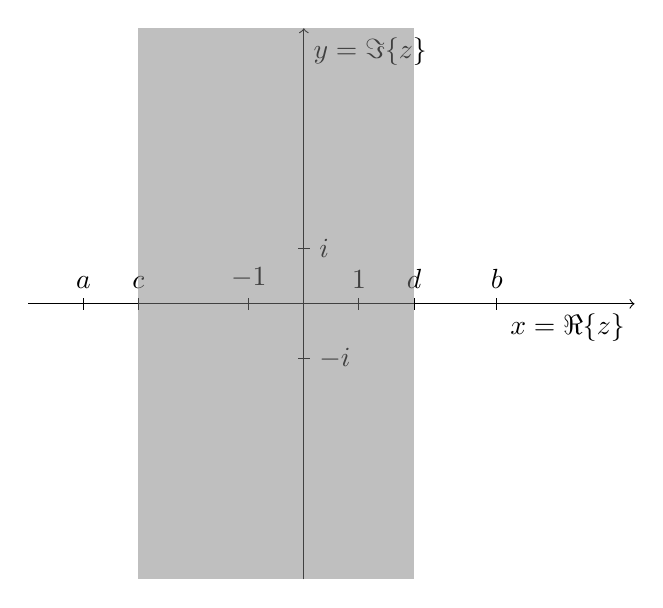
\begin{tikzpicture}
            \begin{scope}[scale=0.7]
            \draw [->] (-5,0) -- (6,0) node [below left]  {$x = \Re\{z\}$};
            \draw [->] (0,-5) -- (0,5) node [below right] {$y = \Im\{z\}$};
        
            \draw (1,-3pt) -- (1,3pt)   node [above] {$1$};
            \draw (-1,-3pt) -- (-1,3pt) node [above] {$-1$};
            \draw (-3pt,1) -- (3pt,1)   node [right] {$i$};
            \draw (-3pt,-1) -- (3pt,-1) node [right] {$-i$};
            \draw (-3,-3pt) -- (-3,3pt) node [above] {$c$};
            \draw (2,-3pt) -- (2,3pt) node [above] {$d$};
            \draw (-4,-3pt) -- (-4,3pt) node [above] {$a$};
            \draw (3.5,-3pt) -- (3.5,3pt) node [above] {$b$};

            \path [draw=none,fill=gray,semitransparent] (-3, -5) rectangle (2, 5);
            \end{scope}
        \end{tikzpicture}\]
        Since $f(z)$ is analytic in this domain, Cauchy's integral theorem tells us that:
        \[
            \oint_{C} f(z) \diff z = 0
        \]
        where $C$ is the boundary of $\Omega$. Splitting $C$ into four pieces:
        \begin{align*}
            \oint_C f(z) \diff z &= \lim_{y\to-\infty}\int_{c}^{d} f(x+iy) \diff x+ \int_{-\infty}^\infty f(d+iy) \diff y  \\
            &\mspace{35mu} + \lim_{y\to\infty} \int_{d}^c f(x+iy) \diff x + \int_{\infty}^{-\infty} f(c+iy) \diff y
        \end{align*}
        The horizontal pieces go to zero since $f\to 0$ on all vertical lines within the strip between $x=a$ and $x=b$. Splitting $f(x+yi) = F(x, y) + iG(x, y)$ into real and imaginary parts gives:
        \[
            \int_{-\infty}^{\infty} F(d, y) + iG(d, y) \diff y - \int_{-\infty}^{\infty} F(c, y) + iG(c, y) \diff y = 0
        \]
        Equating real parts gives:
        \[
            \int_{-\infty}^{\infty} F(d, y) \diff y = \int_{-\infty}^{\infty} F(c, y) \diff y
        \]
        Since $c$ and $d$ are chosen arbitrarily we must have that:
        \[
            \int_{-\infty}^{\infty} F(x,y) \diff y = \textnormal{const.} \qquad (a < x < b)
        \]
        \item Applying the result to $f(z) = e^{z^2}$ gives:
        \[
            \int_{-\infty}^{\infty} \Re\left( e^{(x+iy)^2} \right)\diff y = c \qquad (x,y \textnormal{ real})
        \]
        immediately giving the result:
        \[
            \int_{-\infty}^\infty e^{x^2}\cos(2xy)e^{-y^2} \diff y = c \Longleftrightarrow  \int_{-\infty}^\infty \cos(2xy)e^{-y^2} \diff y = ce^{-x^2}
        \]
        The constant can be found by plugging in $x=0$ and recognizing the classical Gaussian integral:
        \[
            \sqrt{\pi} = \int_{-\infty}^\infty e^{-y^2} \diff y = c
        \]
    \end{enumerate}
\end{solution}

\begin{exercise}
    This exercise gives a neat proof of Cayley's formula for the number of trees of $n$ vertices, by showing more, namely, that there is a pretty formula for the number of such trees even if the degrees of all vertices are specified.
    \begin{enumerate}[label=(\alph*)]
        \item Let $d_1, \ldots, d_n$ be positive integers whose sum is $2n-2$. Show that the number of vertex-labeled trees $T$ of $n$ vertices, in which for all $i=1,\ldots,n$ it is true that $d_i$ is the degree of vertex $i$ of $T$, is exactly 
        \[
            f_n(d_1,\ldots,d_n)=\frac{(n-2)!}{(d_1-1)!(d_2-1)!\cdots (d_n-1)!}
        \]
        (Do this by induction on $n$. show that one of the $d_i$'s, at least, must be $=1$ and go from there.)
        \item Find the generating function 
        \[
            F_n(x_1,\ldots,x_n) = \sum_{\substack{d_1+\cdots+d_n = 2n-2 \\ d_1,\ldots,d_n\geq 1}} f_n(d_1, \ldots, d_n)x_1^{d_1}\cdots x_n^{d_n}
        \]
        in a pleasant, explicit form, involving no summation signs.
        \item Let $x_1=x_2=\cdots=x_n=1$ in your answer to part (b), and thereby prove Cayley's result that there are exactly $n^{n-2}$ labeled trees of $n$ vertices.
        \item Use the sieve method to show that if $e_k$ is the number of vertex labeled trees on $n$ vertices of which $k$ are endpoints (vertices of degree $1$), then 
        \[
            \sum_k e_k x^k = \sum_r \binom{n}{r}r^{n-2}(x-1)^{n-r}
        \]
        \item Show that the average number of endpoints that trees of $n$ vertices have is
        \[
            n\left(1-\frac{1}{n}\right)^{n-2} \sim \frac{n}{e} \quad (n\to\infty)
        \]
        i.e., \emph{the probability that a random vertex of a tree is an endpoint is about $1/e$}.
    \end{enumerate}
\end{exercise}
\begin{solution}
    \begin{enumerate}[label=(\alph*)]
        \item \hypertarget{eq:ch4:18:a}{4.18(a)} Suppose that all $d_i$'s are greater than $1$, then their sum is:
        \[
            \sum_{i=1}^n d_i \geq \sum_{i=1}^n 2 = 2n
        \]
        which is a contradiction, since they have to sum to $2n-2$, hence at least one needs to have degree $1$ (actually, this proof even shows that there must be at least $2$ vertices with degree $1$).

        Now, we proceed by induction on $n$. The base case is obviously true, since there is only one labeled tree with $2$ vertices (with both vertices having degree $1$). 

        Let $n>2$ and assume the formula holds for $n-1$. Let $d_i$ be the vertex whose degree is $1$. This vertex must connect to one of the other vertices of degree $>1$. Let this connecting vertex have index $j$. Removing this edge and vertex $i$ leaves a tree on $n-1$ vertices with degrees $(d_1, \ldots, d_{i-1}, d_{i+1}, \ldots, d_j - 1, \ldots, d_n)$. Summing over all possible $j$ gives (using the formula for the number of labeled trees on $n-1$ vertices given a degree list by the induction hypothesis):
        \[
            f_n(d_1,\ldots,d_n) = \sum_{\substack{1\leq j\leq n \\ d_j \neq 1 \\ i \neq j}} \frac{(n-3)!}{(d_1-1)!\cdots (d_{i-1} - 1)! (d_{i+1} -1)!\cdots (d_j - 2)! \cdots}
        \]
        Multiplying numerator and denominator by $(d_j-1)$:
        \[
            f_n(d_1,\ldots,d_n) = \sum_{\substack{1\leq j\leq n \\ d_j \neq 1 \\ i \neq j}} \frac{(n-3)!(d_j-1)}{(d_1-1)!\cdots (d_{i-1} - 1)! (d_{i+1} -1)!\cdots (d_j - 1)! \cdots}
        \]
        Multiplying denominator by $(d_i-1)! = 1$:
        \[
            f_n(d_1,\ldots,d_n) = \sum_{\substack{1\leq j\leq n \\ d_j \neq 1 \\ i \neq j}} \frac{(n-3)!(d_j-1)}{(d_1-1)!\cdots (d_{i} - 1)!\cdots (d_j - 1)! \cdots (d_n-1)!}
        \]
        Relax the condition on $d_j\neq 1$ since including it in the sum gives a zero term anyway:
        \[
            f_n(d_1,\ldots,d_n) = \sum_{\substack{1\leq j\leq n \\ i \neq j}} \frac{(n-3)!(d_j-1)}{(d_1-1)!\cdots (d_{i} - 1)!\cdots (d_j - 1)! \cdots (d_n-1)!} 
        \]
        Factoring out the common part:
        \[
            f_n(d_1,\ldots,d_n) = \frac{(n-3)!}{(d_1-1)!(d_2-1)! \cdots (d_n-1)!} \sum_{\substack{1\leq j\leq n \\ i \neq j}}(d_j-1)
        \]
        The sum of the degrees is $2n-3$ since the vertex with degree $1$ (at index $i$) is excluded and we therefore get:
        \begin{align*}
            f_n(d_1,\ldots,d_n) &= \frac{(n-3)!}{(d_1-1)!(d_2-1)! \cdots (d_n-1)!} ((2n-3) - (n-1)) \\
            &=  \frac{(n-2)!}{(d_1-1)!(d_2-1)! \cdots (d_n-1)!}
        \end{align*}
        as desired.
        \item The generating function is:
        \[
            F_n(x_1,\ldots,x_n) = \sum_{\substack{d_1+\cdots+d_n = 2n-2 \\ d_1,\ldots,d_n\geq 1}} f_n(d_1, \ldots, d_n)x_1^{d_1}\cdots x_n^{d_n}
        \]
        Let $r_i = d_i - 1$ such that:
        \[
            F_n(x_1,\ldots,x_n) = \sum_{\substack{r_1+\cdots+r_n = n-2 \\ r_1,\ldots,r_n\geq0} } f_n(r_i+1, \ldots, r_n+1)x_1^{r_1+1}\cdots x_n^{r_n+1}
        \]
        Using the multinomial theorem:
        \begin{align*}
            F_n(x_1,\ldots,x_n) \estepalign{\hyperlink{4.18(a)}{4.18(a)}} (x_1x_2\cdots x_n)\sum_{\substack{r_1+\cdots+r_n = n-2 \\ r_1,\ldots,r_n\geq0} } \frac{(n-2)!}{r_1! r_2!\cdots r_n!} x_1^{r_1}\cdots x_n^{r_n} \\
            \estepalign{\ref{ex:2-20}} (x_1x_2\cdots x_n) (x_1+x_2+\ldots+x_n)^{n-2}
        \end{align*}
        \item Letting $x_1=x_2=\cdots=x_n = 1$ gives:
        \[
            \sum_{\substack{d_1+\cdots+d_n = 2n-2 \\ d_1,\ldots,d_n\geq 1}} f_n(d_1, \ldots, d_n) = (1\cdot1\cdots 1)(1+1+\ldots+1)^{n-2} = n^{n-2}
        \]
        \item Let $\Omega$ be the set of all labeled trees on $n$ vertices. There is a property $i$ if a tree has vertex $i$ as endpoint. Let $S$ be a set of endpoints. The number of trees which have all vertices in $S$ as endpoints is:
        \[
            N(\supseteq S) = (n-|S|)^{|S|}(n - |S|)^{n-|S|-2} = (n-|S|)^{n-2}
        \]
        The first factor comes from the possiblities for which each endpoint is connected to. The second term is the number of labeled trees on $(n-|S|)$ vertices. To visualize this construction, start with an arbitrary tree of $(n-|S|)$ vertices, then choose $|S|$ of these vertices (with each vertex possibly chosen multiple times) and then connect the set of endpoints in $S$ to these vertices.
        
        The unfiltered data is therefore:
        \[
            N_r = \sum_{|S| = r} N(\supseteq S) = \binom{n}{r} (n-r)^{n-2}
        \]
        By the sieve method:
        \[
            \bsum[k]  e_k x^k = E(x) \estep{\eqref{eq:sieve}} N(x-1) = \bsum[r] \binom{n}{r} (n-r)^{n-2}(x-1)^r
        \]
        After a change of variables
        \[
            \bsum[k]  e_k x^k = \bsum[r] \binom{n}{r} r^{n-2}(x-1)^{n-r}
        \]
        \item The average number of endpoints is given by $E'(1) / E(1)$ which is equal to:
        \begin{align*}
            \frac{E'(1)}{E(1)} = \frac{\binom{n}{n-1}(n-1)^{n-2}}{\binom{n}{n}n^{n-2}} = n\left(1 - \frac{1}{n}\right)^{n-2}  \sim n e^{-1} = \frac{n}{e}
        \end{align*}
    \end{enumerate}
\end{solution}

\begin{exercise}
    \begin{enumerate}[label=(\alph*)]
        \item If $N(\subseteq S)$ is the number of objects whose set of properties is contained in $S$, then for all sets $T$, the number of objects whose set of properties is \emph{precisely} $T$ is
        \[
            N(=T) = \sum_{S\subseteq T} (-1)^{|S| - |T|} N(\subseteq S)
        \]
        \item Let $S$ be a fixed set of positive integers, and let $h_n(S)$ be the number of hands of weight $n$, in a certain labeled exponential family, whose card sizes all belong to $S$. Find the egf of $\{h_n(S)\}$.
        \item Multiply by $(-1)^{|S|-|T|}$ and sum over $S\subseteq T$ to find the egf of $\{\psi_n(T)\}_{n\geq0}$, the number of hands whose set of distinct card sizes is \emph{exactly} $T$, in the form (the $d$'s are the deck sizes)
        \[
            \sum_{n\geq0} \frac{\psi_n(T)}{n!} x^n = \prod_{t\in T} \left(e^{\frac{d_tx^t}{t!}} - 1 \right)
        \]
        \item Let $\rho(n,k)$ be the number of hands of weight $n$ that have exactly $k$ different \emph{sizes} of cards (however many cards they might have!). Sum the result of (c) over all $|T|=k$, etc., to find that 
        \[
            \sum_{n,k\geq0} \frac{\rho(n,k)}{n!} x^n y^k = \prod_{t\geq1}\left\{1+y\left(e^{d_tx^t/t!}-1\right)\right\}
        \]
        \item Let $c_n$ be the average number of different sizes of cycles that occur in permutations of $n$ letters. Show that the opsgf of $\{c_n\}$ is 
        \[
            \frac{1}{1-x}\sum_{t\geq1} \left(1-e^{-x^t/t}\right)
        \]
        and find an explicit formula for $c_n$.
    \end{enumerate}
\end{exercise}
\begin{solution}
    \begin{enumerate}[label=(\alph*)]
        \item \hypertarget{eq:ch4:19:a}{} Note that:
        \[
            N(\subseteq S) = \sum_{U \subseteq S} N(=U)
        \]
        Starting from the right-hand side, we then have:
        \begin{align*}
            \sum_{S\subseteq T} (-1)^{|S| - |T|} N(\subseteq S) &= \sum_{S\subseteq T} (-1)^{|S| - |T|}\sum_{U \subseteq S} N(=U) \\
            &= \sum_{U \subseteq T} N(=U)  \sum_{U\subseteq S\subseteq T}(-1)^{|S| - |T|}
        \end{align*}
        Note that the inner sum can be rewritten as looping over all subsets $W$ of $T\setminus U$ (and compensating $|S|$ to be $|W| + |U|$):
        \[
            \sum_{S\subseteq T} (-1)^{|S| - |T|} N(\subseteq S) =  \sum_{U \subseteq T} N(=U) (-1)^{|U| - |T|} \sum_{W \subseteq T \setminus U}(-1)^{|W|}
        \]
        The inner sum is equivalent to:
        \[
            \sum_{W \subseteq T \setminus U}(-1)^{|W|} = \sum_{r=0}^{|T|-|U|} \binom{|T| - |U|}{r} (-1)^r
        \]
        which is $0$ for $|T| - |U| \neq 0$ by the binomial theorem and $1$ if $|T| - |U| = 0$:
        \[
            \sum_{W \subseteq T \setminus U}(-1)^{|W|} = \delta_{|T|, |U|}
        \]
        Plugging this back in yields:
        \[
            \sum_{S\subseteq T} (-1)^{|S| - |T|} N(\subseteq S) =  \sum_{U \subseteq T} N(=U) (-1)^{|U| - |T|} \delta_{|T|, |U|}
        \]
        But the only subset of $|T|$ which has the same size as $|T|$ is $|T|$ itself:
        \[
            \sum_{S\subseteq T} (-1)^{|S| - |T|} N(\subseteq S) = N(=T)(-1)^{|T|-|T|} = N(=T)
        \]
        \item \hypertarget{eq:ch4:19:b}{} Consider the same exponential family with only the $d_s$ where $s\in S$. Its deck enumerator is:
        \[
            \mathcal{D}_S(x) = \sum_{s\in S} d_s \frac{x^s}{s!}
        \]
        From the exponential formula, we then have:
        \begin{align*}
            \bsum[n] h_n(S) \frac{x^n}{n!} = \exp(\mathcal{D}_S(x)) = \prod_{s\in S} \exp\left(d_s \frac{x^s}{s!} \right)
        \end{align*}
        \item \hypertarget{eq:ch4:19:c}{} Multiplying by $(-1)^{|S|-|T|}$ and summing over $S\subseteq T$ gives:
        \[
            \sum_{S\subseteq T}\bsum (-1)^{|S|-|T|}h_n(S) \frac{x^n}{n!} \estep{\hyperlink{eq:ch4:19:b}{4.19(b)}} \sum_{S\subseteq T} (-1)^{|S|-|T|} \prod_{s\in S} \exp\left(d_s \frac{x^s}{s!} \right)
        \]
        The left-hand side of this equality is just the egf of $\{\psi_n(T)\}_{n\geq0}$ by part \hyperlink{eq:ch4:19:a}{4.19(a)}. Now we show that the right-hand side is:
        \[
            \prod_{t\in T} \left(\exp\left(\frac{d_tx^t}{t!}\right) - 1\right)
        \]
        by induction on the size of $|T|$.

        For the base case, let $T = \{t_1\}$ be a set of one element. Then we have that:
        \begin{align*}
            \sum_{S\subseteq T} (-1)^{|S|-|T|} \prod_{s\in S} \exp\left(\frac{d_s x^s}{s!} \right) &= (-1)^{0}\prod_{s\in \{t_1\}} \exp\left( \frac{d_tx^t}{t!}\right) + (-1)^{-1} \cdot 1 \\
            &= \prod_{t\in T}\left(\exp\left(\frac{d_tx^t}{t!}\right) - 1\right)
        \end{align*}
        where we used the fact that there are only two subsets of $T$ in the first equality. For ease of notation, let:
        \[
            P(S) = \prod_{s\in S} \exp\left(\frac{d_s x^s}{s!}\right)
        \]
        Now let $T$ be a set of $n$ elements and assume that 
        \[
            \sum_{S\subseteq T'} (-1)^{|S|-|T'|} P(S) = \prod_{t\in T'} \left(\exp\left(\frac{d_tx^t}{t!}\right) - 1\right)
        \]
        for any set $T'$ of $n-1$ elements.
        We do this by splitting the sum in subsets which contain $t_1$ and subsets which do not contain $t_1$ (where $t_1\in T$):
        \begin{align*}
            \sum_{S\subseteq T} (-1)^{|S|-|T|} P(S) &= \sum_{S\subseteq T\setminus \{t_1\}} (-1)^{|S| + 1 - |T|} \exp\left(\frac{d_{t_1}x^{t_1}}{t_1!}\right)P(S)\\
            &\mspace{50mu}+  \sum_{S\subseteq T\setminus \{t_1\}} (-1)^{|S| - |T|} P(S) \\
            &= \exp\left(\frac{d_{t_1}x^{t_1}}{t_1!}\right) \sum_{S\subseteq T'} (-1)^{|S| - |T'|} P(S)  \\
            &\mspace{50mu} - \sum_{S\subseteq T'} (-1)^{|S| - |T'|} P(S)
        \end{align*}
        Where $T' = T\setminus \{t_1\}$. Applying the induction hypothesis gives the desired result:
        \begin{align*}
            \sum_{S\subseteq T} (-1)^{|S|-|T|} P(S) &= \left(\exp\left(\frac{d_{t_1}x^{t_1}}{t_1!}\right) - 1\right)\prod_{t\in T'} \left(\exp\left(\frac{d_tx^t}{t!}\right) - 1\right) \\
            &=\prod_{t\in T} \left(\exp\left(\frac{d_tx^t}{t!}\right) - 1\right)
        \end{align*}
        We have therefore shown that:
        \[
            \bsum \frac{\psi_n(T)}{n!} x^n = \prod_{t\in T} \left(\exp\left(\frac{d_tx^t}{t!}\right) - 1 \right)
        \]
        \item Summing the result of part (c) over all $|T| = k$, multiplying by $y^k$ and summing over $k$:
        \[
            \bsum[k] \sum_{|T| = k} \bsum[n] \frac{\psi_n(T)}{n!}x^ny^k =\bsum[k] \sum_{|T|=k} \left\{\prod_{t\in T}\left(e^{\frac{d_tx^t}{t!}} - 1 \right)\right\}y^k
        \]
        On the left side we can use $\sum_{|T| = k} \psi_n(T) = \rho(n,k)$. For the right-hand side we start by moving $y$ inside (using $|T|=k$):
        \[
            \bsum[k] \sum_{|T|=k} \left\{\prod_{t\in T}\left(e^{\frac{d_tx^t}{t!}} - 1 \right)\right\}y^k = \bsum[k] \sum_{|T|=k} \left\{\prod_{t\in T}y\left(e^{\frac{d_tx^t}{t!}} - 1 \right)\right\}
        \]
        but the two summations just sum over all possible sets which can also be written as:
        \[
            \bsum[k] \sum_{|T|=k} \left\{\prod_{t\in T}y\left(e^{\frac{d_tx^t}{t!}} - 1 \right)\right\} = \prod_{t=1}^\infty \left\{ 1+y\left(e^{d_tx^t/t!} - 1\right)\right\}
        \]
        which has the semantics of either not choosing an element (the $1$) or choosing an element (the term with $y$). The result now follows:
        \[
            \bsum[n]\bsum[k] \rho(n,k) \frac{x^n}{n!} y^k = \prod_{t=1}^\infty\left\{1+y\left(e^{d_tx^t/t!}-1\right)\right\}
        \]
        \item In the exponential family for permutations and their cycles, we have $d_n = (n-1)!$ and therefore by the previous part:
        \[
            \bsum[n]\bsum[k] \frac{\rho(n,k)}{n!} x^n y^k = \prod_{t=1}^\infty\left\{1+y\left(\exp\left(\frac{x^t}{t}\right)-1\right)\right\}
        \]
        which is the enumerator for the number of permutations of $n$ letters with $k$ different cycles. Now taking the derivative with respect to $y$ and evaluating at $y=1$ gives exactly the opsgf of $c_n$ on the left-hand side:
        \[
            \bsum[n]\bsum[k] k\frac{\rho(n,k)}{n!} x^n = \bsum[n] c_n x^n = C(x)
        \]
        Applying the same operation to the right-hand side:
        \begin{align*}
            C(x) &= \frac{\partial}{\partial y} \prod_{t=1}^\infty\left\{1+y\left(\exp\left(\frac{x^t}{t}\right)-1\right)\right\}\bigg\rvert_{y=1} \\
            &= \sum_{t=1}^\infty \left(\exp\left(\frac{x^t}{t}\right)-1\right) \prod_{\substack{t'\geq 1\\ t'\neq t}}\left\{1+y\left(\exp\left(\frac{x^{t'}}{t'}\right)-1\right)\right\}\bigg\rvert_{y=1} 
            \\
            &= \sum_{t=1}^\infty \left(\exp\left(\frac{x^t}{t}\right)-1\right) \prod_{\substack{t'\geq 1\\ t'\neq t}}\left\{\exp\left(\frac{x^{t'}}{t'}\right)\right\}
        \end{align*}
        where we used the product rule for differentiation in the second equality. Working this out further yields
        \begin{align*}
            C(x) &=  \sum_{t=1}^\infty \left(\exp\left(\frac{x^t}{t}\right)-1\right) \exp\left(-\frac{x^t}{t}\right)\prod_{t'= 1}^\infty\left\{\exp\left(\frac{x^{t'}}{t'}\right)\right\} \\
            &= \sum_{t=1}^\infty \left(\exp\left(\frac{x^t}{t}\right)-1\right) \exp\left(-\frac{x^t}{t}\right)\exp\left\{{\sum_{t'=1}^\infty \frac{x^{t'}}{t'}}\right\}
        \end{align*}
        In the exponent, the power series of $\log \frac{1}{1-x}$ is recognized, see \eqref{eq:power_loggeom}, yielding:
        \[
            C(x) = \frac{1}{1-x}\sum_{t=1}^\infty \left(1-\exp\left(-\frac{x^t}{t}\right)\right)
        \]
        For an explicit formula for $c_n$ we need to extract the coefficient of $x^n$. Since multiplying by $\frac{1}{1-x}$ extracts the sequence of partial sums, we are interested in:
        \[
            c_n = \sum_{j=0}^n \coeff{x^j} \sum_{t= 1}^\infty \left(1-\exp\left(-\frac{x^t}{t}\right)\right)
        \]
        The coefficient of $x^j$ is given by:
        \begin{align*}
            \coeff{x^j} \sum_{t=1}^\infty \left(1-\exp\left(-\frac{x^t}{t}\right)\right) \estepalign{\eqref{eq:power_exp}} \coeff{x^j} \sum_{t=1}^\infty \sum_{k= 1}^\infty \frac{(-1)^{k+1}x^{kt}}{t^k k!} \\
            &= \begin{cases}
                \sum_{m|j} \frac{(-1)^{m+1}}{(j/m)^m m!} & j\neq 0 \\
                0 & j = 0
            \end{cases}
        \end{align*}
        such that:
        \[
            c_n = \sum_{j=1}^n \sum_{m\vert j} \frac{(-1)^{m+1}}{(j/m)^m m!}
        \]
    \end{enumerate}
\end{solution}

\begin{exercise}
    Begin with the set $\{1, 2, \ldots, n\}$. Toss a coin $n$ times, once for each member of the set. Keep the elements that scored `Heads' and discard the elements that got `Tails'. You now have a certain subset $S$ of the original set. Call this whole process a `step'. Now take a step from $S$. That is, toss a coin for each element of $S$, and keep those that get `Heads', getting a sub-subset $S'$, etc.\ The game halts when the empty set is reached. Let $f(n,k,r)$ be the probability that after $k$ steps, exactly $r$ objects remain.
    \begin{enumerate}[label=(\alph*)]
        \item Find a recurrence relation for $f$, find the generating function for $f$, and find $f$ itself.
        \item What is the \emph{average} number of steps in a complete game?
        \item What is the standard deviation of the number of steps in the game?
    \end{enumerate}
\end{exercise}
\begin{solution}
    \begin{enumerate}[label=(\alph*)]
        \item The probability that after $k$ steps exactly $r$ coins remain starting with $n$ coins is the following sum (advance from $k-1$ to $k$, choose a subset of size $r$, toss heads for all of these, toss heads for the rest, multiply by the possible number of ways):
        \[
            f(n,k,r) = \sum_{r'=r}^{n} f(n, k - 1, r') \binom{r'}{r} \frac{1}{2^{r'}} =  \bsum[r'] f(n, k - 1, r') \binom{r'}{r} \frac{1}{2^{r'}}
        \]
        for $k\geq 1$, where we used the fact that $\binom{n}{k} = 0$ for $n < k$ as well as $f(n,k-1,r') = 0$ for $r'>n$. At $k=0$, we have the following identity:
        \[
            f(n,0,r) = \delta_{n,r}
        \]
        Define $F_{k,r}(x) = \bsum f(n,k,r) x^n$ and note that $F_{0,r}(x) = x^r$. Multiplying both sides of the recurrence by $x^n$ and summing over $n$ gives:
        \[
            F_{k,r}(x) = \bsum[n] \bsum[r'] f(n,k-1,r') \binom{r'}{r} \frac{1}{2^{r'}} x^n = \bsum[r'] F_{k-1,r'} \binom{r'}{r} \frac{1}{2^{r'}}
        \]
        Starting from:
        \[ 
            F_{0,r} = x^r 
        \]
        we then get:
        \[
            F_{1,r} = \bsum[r'] \left(\frac{x}{2}\right)^{r'} \binom{r'}{r} \estep{\eqref{eq:binom_denom_num_single}} \frac{\left(\frac{x}{2}\right)^r}{\left(1-\frac{x}{2}\right)^{r+1}} = \frac{2}{2-x} \left(\frac{x}{2-x}\right)^{r}
        \]
        \begin{align*}
            F_{2,r} &= \frac{2}{2-x}\bsum[r'] \left(\frac{x}{2-x}\right)^{r'} \binom{r'}{r} \frac{1}{2^{r'}} \estep{\eqref{eq:binom_denom_num_single}} \frac{2}{2-x} \frac{\left(\frac{x}{4-2x}\right)^r}{\left(1-\frac{x}{4-2x}\right)^{r+1}} \\
            &= \frac{2}{2-x}\frac{4-2x}{4-3x} \left(\frac{x}{4-3x}\right)^{r} = \frac{4}{4-3x}\left(\frac{x}{4-3x}\right)^{r}
        \end{align*}
        This suggests a general form:
        \[
            F_{k,r}(x) = \frac{2^{k}}{2^k - (2^k - 1)x}\left(\frac{x}{2^k - (2^k-1)x}\right)^r = \frac{2^k x^r}{(2^k - (2^k-1)x)^{r+1}}
        \]
        We show this by induction on $k$:
        \begin{align*}
            F_{k,r} &= \frac{2^{k-1}}{2^{k-1} - (2^{k-1} - 1)x} \bsum[r'] \left(\frac{x}{2^{k-1} - (2^{k-1}-1)x}\right)^{r'} \binom{r'}{r} \frac{1}{2^{r'}} \\
            &=\frac{2^{k-1}}{2^{k-1} - (2^{k-1} - 1)x} \bsum[r'] \left(\frac{x}{2^{k} - (2^{k}-2)x}\right)^{r'} \binom{r'}{r} \\
            \estepalign{\eqref{eq:binom_denom_num_single}} \frac{2^{k-1}}{2^{k-1} - (2^{k-1} - 1)x} \left(\frac{\left(\frac{x}{2^k-(2^k - 2)x}\right)^r}{\left(1-\frac{x}{2^k-(2^k-2)x}\right)^{r+1}}\right) \\ 
            &= \frac{2^{k-1}}{2^{k-1} - (2^{k-1} - 1)x} \frac{2(2^{k-1} - (2^{k-1}-1)x)}{2^k - (2^k -1)x}\left(\frac{x}{2^k - (2^k-2)x - x}\right)^r \\
            &= \frac{2^k}{2^k - (2^k - 1)x} \left(\frac{x}{2^k - (2^k-1)x}\right)^r \\
            &=  \frac{2^k x^r}{(2^k - (2^k-1)x)^{r+1}}
        \end{align*}
        $f(n,k,r)$ is then easily found from taking the coefficient $\coeff{x^n}F_{k,r}(x)$:
        \begin{align*}
            f(n,k,r) &= \coeff{x^{n-r}} \frac{2^{k}}{2^{k(r+1)} (1 - (1-2^{-k})x)^{r+1}} \\
            \estepalign{\eqref{eq:binom_denom}} 2^{-kr} \coeff{x^{n-r}} \infsum[m] \binom{m+r}{m} (1-2^{-k})^m x^m \\
            &= 2^{-kr} \binom{n}{n-r}(1-2^{-k})^{n-r}
        \end{align*}
        \item To calculate the average, we first calculate the probability that a game ends after $k$ tosses. This is given by:
        \[
            p_{n}(k) = \sum_{r=1}^\infty f(n, k-1, r) \frac{1}{2^r}
        \]
        since in the last step all coins must be eliminated.
        
        Working this out with the previously found formula gives:
        \begin{align*}
            p_n(k) &= \sum_{r=1}^n 2^{-(k-1)r} \binom{n}{n-r} (1-2^{-k+1})^{n-r} 2^{-r} \\
            &= \sum_{r=1}^n \binom{n}{n-r} \left(2^{-k}\right)^r (1-2^{-k+1})^{n-r}
        \end{align*}
        This is just the binomial theorem \eqref{eq:binom_num2} where the term with $r=0$ is omitted:
        \begin{align*}
            p_n(k) &= \left(1-2^{-k+1} + 2^{-k}\right)^n - \left(1-2^{-k+1}\right)^n \\
            &= \left(1-2^{-k}\right)^n - \left(1-2^{-k+1}\right)^n
        \end{align*}
        The average number of steps to complete the game is now given by:
        \[
            \mu_n = \bsum[k] kp_n(k) = \bsum[k] k \left\{\left(1-2^{-k}\right)^n - \left(1-2^{-k+1}\right)^n \right\}
        \]
        To get a finite summation, we use a different formulation. Let $X$ be the random variable denoting the number of steps in a game. Since $X$ is positive, we can use:
        \[
            \mu_n = \bsum[k] P(X > k)
        \]
        The probability that $X > k$ is given by:
        \[
           P(X > k) = 1 - f(n, k, 0)
        \]
        since $f(n, k, 0)$ gives the probability that the game has ended after the $k$th turn. Filling this in, we get:
        \begin{align*}
            \mu_n &= \bsum[k] 1 - f(n,k,0) = \bsum[k] 1 - (1-2^{-k})^n \estep{\eqref{eq:binom_num}} \bsum[k] \sum_{m=1}^n \binom{n}{m} \frac{(-1)^{m+1}}{2^{mk}} \\
            &= \sum_{m=1}^n \binom{n}{m} (-1)^{m+1}  \bsum[k] 2^{-mk} \estep{\eqref{eq:power_geom}} \sum_{m=1}^n \binom{n}{m} (-1)^{m+1} \frac{1}{1-2^{-m}}
        \end{align*}
        Both of these formulations can also be found in \href{https://oeis.org/A158466}{OEIS A158466}.
        \item The variance is given by:
        \[
            \sigma^2_n = \left\{\bsum[k] k^2 p_n(k)\right\} - \mu^2_n
        \]
        where the first term is
        \[
            \bsum[k] k^2 p_n(k) = \bsum[k] k^2 \left\{(1-2^{-k})^n - (1-2^{-k+1})^n\right\}
        \]
        Again, we can formulate a finite sum by using the identity
        \[
            \bsum[k] k^2 p_n(k) = \bsum[k] (2k+1)P(X > k)
        \]
        where $\bsum[k] P(X>k)$ has already been calculated in the previous part and we only require
        \[
            \bsum[k] 2k P(X > k) = \bsum[k] 2k(1-f(n,k,0)) = \bsum[k] 2k (1 - (1-2^{-k})^n)
        \]
        which we find from a similar calculation:
        \begin{align*}
            \bsum[k] 2k P(X>k) \estepalign{\eqref{eq:binom_num}} \bsum[k] 2k \sum_{m=1}^n \binom{n}{m} \frac{(-1)^{m+1}}{2^{mk}} \\
            &= \sum_{m=1}^n 2 \binom{n}{m} (-1)^{m+1} \bsum[k] \frac{k}{2^{mk}} x^k \bigg\rvert_{x=1} \\
            \estepalign{\eqref{eq:xD}} \sum_{m=1}^n 2 \binom{n}{m}(-1)^{m+1} xD \bsum[k] \left(\frac{x}{2^m}\right)^k \bigg\rvert_{x=1} \\
            \estepalign{\eqref{eq:power_geom}} \sum_{m=1}^n2\binom{n}{m}(-1)^{m+1} xD\frac{1}{1 - x2^{-m}}\bigg\rvert_{x=1} \\
            &= \sum_{m=1}^n \binom{n}{m}(-1)^{m+1} \frac{2\cdot 2^{m}}{(2^m-1)^2}
        \end{align*}
        To conclude, we have that:
        \begin{align*}
            \bsum[k] k^2 p_n(k) &= \sum_{m=1}^n \binom{n}{m} (-1)^{m+1} \left\{\frac{2^{m+1}}{(2^m - 1)^2} + \frac{1}{1-2^{-m}} \right\} \\
            &= \sum_{m=1}^n \binom{n}{m} (-1)^{m+1} \frac{2^m - 4^m}{(2^m - 1)^2}
        \end{align*}
        and the standard deviation given by
        \[
            \sigma_n = \sqrt{\sum_{m=1}^n \left[\binom{n}{m} (-1)^{m+1} \frac{2^m - 4^m}{(2^m - 1)^2}\right] -\left[\sum_{m=1}^n \binom{n}{m} (-1)^{m+1} \frac{2^m}{2^m-1}\right]^2}
        \]
    \end{enumerate}
\end{solution}

\begin{exercise}
    Let $f(n,k,t)$ be the number of HC-polyominoes that have $n$ cells, in $k$ layers, the highest layer consisting of exactly $t$ cells. Show that the `grand' three-variable generating function is
    \[
        \sum_{n,k,t} f(n,k,t)x^ny^kz^t = \frac{xyz(1-x)^2((1-xz)(1-x)^2+x^2y(z-1))}{(1-xz)^2((1-x)^4-xy(1-x-x^2+x^3+x^2y))}
    \]
\end{exercise}
\begin{solution}
    We first list the known results which we will use (see the main text for the derivations). Denote $F_{k,t}(x) = \sum_n f(n,k,t)x^n$ with $F_{1,t} = x^t$ which satisfies:
    \[
        F_{k,t}(x) = x^t (V_{k-1}(x) +(t-1)U_{k-1}(x)) \qquad (k\geq 2)
    \]
    where $U_k(x) = \sum_{r=1}^\infty F_{k,r}(x)$ and $V_k(x)= \sum_{r=1}^\infty rF_{k,r}(x)$ with initial values $U_1(x) = x/(1-x)$, $V_1(x) = x/(1-x)^2$ and $U_0(x) = V_0(x) = 0$. These satisfy the simultaneous recurrences:
    \begin{align*}
        U_k(x) &= \frac{x}{1-x} V_{k-1}(x) + \frac{x^2}{(1-x)^2}U_{k-1}(x)  \qquad\mspace{3mu}(k\geq 2) \\
        V_k(x) &= \frac{x}{(1-x)^2}V_{k-1}(x) + \frac{2x^2}{(1-x)^3}U_{k-1}(x)\quad  (k\geq 2)
    \end{align*}
    We also have the generating function:
    \[
        \phi(x,y) = \bsum[k] U_k(x)y^k = \frac{xy(1-x)^3}{(1-x)^4-xy(1-x-x^2+x^3+x^2y)}
    \]
    Now define the generating function:
    \[
        \psi(x, y) = \bsum[k] V_k(x)y^k
    \]
    which we find by multiplying the recurrence for $U_k(x)$ by $y^k$ and summing over $k\geq 2$:
    \[
        \phi(x,y) - \frac{xy}{1-x} = \frac{xy}{1-x}\psi(x,y) + \frac{x^2y}{(1-x)^2}\phi(x,y)
    \]
    Solving for $\psi(x,y)$ gives:
    \[
        \psi(x,y) = \left(\frac{(1-x)^2 -x^2y}{xy(1-x)}\right)\phi(x,y) - 1
    \]
    Multiplying the recurrence for $F_{k,t}(x)$ by $y^kz^t$ and summing over $k\geq 2$ and $t\geq 1$ yields:
    \[
        \sum_{k=2}^\infty\sum_{t=1}^\infty F_{k,t}(x)y^kz^t =\sum_{k=2}^\infty\sum_{t=1}^\infty x^t(V_{k-1}(x) + (t-1)U_{k-1}(x))y^kz^t
    \]
    We rewrite the left-hand side in terms of the wanted generating function:
    \begin{align*}
        \textnormal{l.h.s.} &= \sum_{t=1}^\infty\sum_{k=1}^\infty F_{k,t}(x)y^kz^t  - \sum_{t=1}^\infty F_{1,t}(x)yz^t \\
        &= \sum_{t=1}^\infty\sum_{k=1}^\infty F_{k,t}(x)y^kz^t - \sum_{t=1}^\infty x^tyz^t \\
        \estepalign{\eqref{eq:power_geom}} F(x,y,z) - \frac{y}{1-xz} + y  \\
        &= F(x,y,z) - \frac{xyz}{1-xz}
    \end{align*}
    where we also used the fact that $f(n,k,t)=0$ whenever $k=0$ or $t=0$.
    For the right side, swap the summations to recognize $\psi(x,y)$ and $\phi(x,y)$:
    \begin{align*}
        \textnormal{r.h.s.} &= \sum_{t=1}^\infty x^tz^t \bigg\{\sum_{k=2}^\infty V_{k-1}(x)y^k + (t-1)\sum_{k=2}^\infty U_{k-1}(x)y^k\bigg\} \\
        &=\sum_{t=1}^\infty x^tz^t \left(y\psi(x,y) + (t-1)y\phi(x,y)\right) \\
        &= \frac{xyz}{1-xz}\psi(x,y) + \frac{xyz}{(1-xz)^2}\phi(x,y) - \frac{xyz}{1-xz}\phi(x,y)\\
        &=  \frac{xyz}{1-xz}\psi(x,y) + \frac{yx^2z^2}{(1-xz)^2} \phi(x,y) 
    \end{align*}
    where in the third equality we used the identities
    \[
        C\sum_{t=1}^\infty x^tz^t \estep{\eqref{eq:power_geom}} C \left(\frac{1}{1-xz} - 1\right) = \frac{Cxz}{1-xz}
    \]
    and
    \[
        C\sum_{t=1}^\infty tx^tz^t \estep{\eqref{eq:xD}} C xD_x\sum_{t=1}^\infty x^tz^t = xD_x \frac{Cxz}{1-xz} = \frac{Cxz}{(1-xz)^2}
    \]
    where $C$ is an expression which is constant with respect to $t$ and $D_x$ denotes differentation with respect to $x$.
    Combining this with the left-hand side, we obtain:
    \[
        F(x,y,z) = \frac{xyz}{1-xz}(\psi(x,y) + 1) + \frac{yx^2z^2}{(1-xz)^2} \phi(x,y)
    \]
    We start by filling in $\psi(x,y)$ and doing some algebraic manipulations:
    \begin{align*}
        F(x,y,z) &= \frac{xyz}{1-xz} \left\{\left(\frac{(1-x)^2 -x^2y}{xy(1-x)}\right)\phi(x,y) - 1 + 1\right\}  + \frac{yx^2z^2}{(1-xz)^2} \phi(x,y) \\
        &= \frac{z(1-x)^2 -x^2yz}{(1-xz)(1-x)}\phi(x,y) + \frac{yx^2z^2}{(1-xz)^2}\phi(x,y) \\
        &= \frac{(1-xz) \left(z(1-x)^2 - x^2yz\right)+ yx^2z^2 - yx^3z^2}{(1-xz)^2(1-x)}\phi(x,y) \\
        &= \frac{z((1-xz)(1-x)^2 - (1-xz)x^2y + yx^2z -yx^3z)}{(1-xz)^2(1-x)}\phi(x,y) \\
        &= \frac{z((1-xz)(1-x)^2 + x^2y(z-1))}{(1-xz)^2(1-x)}\phi(x,y)
    \end{align*}
    Lastly, we fill in $\phi(x,y)$ to obtain the final result:
    \begin{align*}
        F(x,y,z) &= \frac{z((1-xz)(1-x)^2 + x^2y(z-1))\left\{xy(1-x)^3\right\}}{(1-xz)^2(1-x) \left\{(1-x)^4-xy(1-x-x^2+x^3+x^2y) \right\}} \\
        &= \frac{xyz(1-x)^2((1-xz)(1-x)^2+x^2y(z-1))}{(1-xz)^2((1-x)^4-xy(1-x-x^2+x^3+x^2y))}
    \end{align*}
\end{solution}

\begin{exercise}
    Let $(a_1, b_1)$, \ldots, $(a_k, b_k)$ be an exact covering sequence. Show that 
    \[
        \sum_{j : a_j \textnormal{ is even}} \frac{1}{b_j} = \frac{1}{2} = \sum_{j : a_j \textnormal{ is odd}} \frac{1}{b_j}
    \]
    Generalize this result to other residue classes for the $a_j$.
\end{exercise}
\begin{solution}
    The statement is incorrect, consider the ECS $\{(0, 3)$, $(1, 3)$, $(2, 3)\}$.

    However if all $b_j$ are even, the statement does hold. Indeed, since the polynomial $\psi_2(z) = \sum_{j:2\vert b_j} \frac{z^{a_j}}{b_j} = \sum_{j=1}^k \frac{z^{a_j}}{b_j}$ is divisible by the cyclotomic polynomial $\Phi_2(z)$, we find that:
    \[
        \psi_2(-1) = \sum_{j=1}^k \frac{(-1)^{a_j}}{b_j} = \sum_{j:a_j \textnormal{ is even}} \frac{1}{b_j} -  \sum_{j:a_j \textnormal{ is odd}} \frac{1}{b_j} = 0
    \]
    and since $\sum_{j=1}^k \frac{1}{b_j} = 1$, the result follows.

    For general residue classes of $a_j$, let every $b_j$ be divisble by $n$. Then the polynomial
    \[
        \psi_n(z) = \sum_{j:n \vert b_j} \frac{z^{a_j}}{b_j} = \sum_{j=1}^k \frac{z^{a_j}}{b_j}
    \]
    is divisble by $\Phi_n(z)$. Evaluating this at the roots of unity, together with the fact that$ \sum_{j=1}^k \frac{1}{b_j} = 1$ gives rise to the equations:
    \[
        \begin{pmatrix}
            1 & 1 & \cdots & 1 \\
            1 & \omega_n^1 & \cdots & \omega_n^{n-1} \\
            \vdots & \vdots &\ddots & \vdots \\
            1 & \omega_n^{n-1} & \cdots & \omega_n^{(n-1)(n-1)}
        \end{pmatrix} \begin{pmatrix}
            x_0 \\ x_1 \\ \vdots \\ x_{n-1}
        \end{pmatrix} = \begin{pmatrix}
            1 \\ 0 \\ \vdots \\ 0
        \end{pmatrix}
    \]
    where
    \[
        x_i = \sum_{j: a_j \bmod n = i} \frac{1}{b_j}
    \]
    This matrix is just the DFT and inverting gives the desired result:
    \[
        x_0 = x_1 = \cdots = x_{n-1} = \frac{1}{n}
    \]
    (first column of IDFT matrix).
\end{solution}

\begin{exercise}
    What is the probability that a random permutation has equal number of $r$-cycles and $s$-cycles? Express your answer in terms of Bessel functions. Make a table of your answer, as a function of $r$ and $s$, for $1 < r < s \leq 6$.
\end{exercise}
\begin{solution}
    The probability that a random permutation has exactly $j$ $r$-cycles and $j$ $s$-cycles is:
    \[
        \frac{e^{-1/r-1/s}}{r^{j}s^j j!^2}
    \]
    The required probability is then found by summing over all $j$.
    \[
        e^{-1/r-1/s} \sum_{j=0}^\infty \frac{1}{(rs)^j j!^2} = e^{-1/r-1/s} I_0\left(\frac{2}{\sqrt{rs}}\right)
    \]
    where $I_0$ is the modified Bessel function of the first kind:
    \[
        I_0(z) = \sum_{k=0}^\infty \frac{\left(\frac{1}{4}z^2\right)^k}{(k!)^2}
    \]
    Some values are listed in following Table:
    \begin{table}[hbpt]
        \centering
        \begin{NiceTabular}{@{}wr{0.3cm}rrrrr@{}}
            \toprule
            \diagbox{$r$}{$s$} & $2$ & $3$ & $4$ & $5$ & $6$ \\ \midrule
            $1$ & $0.34944$ & $0.35906$ & $0.36273$  &$0.36451$ & $0.36551$ \\
            $2$ & & $ 0.51011$ & $0.53328 $ & $0.54750 $ &  $0.55710 $\\ 
            $3$ & & & $0.60552 $& $0.62641 $ & $0.64070$ \\
            $4$ & & &  & $0.66991$ & $ 0.68700$ \\
            $5$ & & & & & $0.71634$\\
            \bottomrule
        \end{NiceTabular}
    \end{table}
\end{solution}

\begin{exercise}
    Find a three term recurrence relation, whose coefficients are polynomials in $n$, that is satisfied by the quantity
    \[
        (2n+11)4^n  -4(2n+1)\binom{2n}{n},
    \]
    which is the number of convex polyominoes of perimeter $2n+8$.
\end{exercise}
\begin{solution}
    We use Maple to simplify some calculations which could also be done manually. First, the generating function of the sequence is:
\begin{mapleinput}
%\prompt% F := sum(x^n*((2*n+11)*4^n - 
  4*(2*n+1)*binomial(2*n,n)), n=0..infinity, formal);
\end{mapleinput} \begin{mapleoutput}
    \[F\coloneqq \frac{8 x}{\left(4 x-1\right)^{2}}-\frac{11}{4 x-1}-\frac{16 x}{\left(-4 x+1\right)^{\frac{3}{2}}}-\frac{4}{\sqrt{-4 x+1}}\]
\end{mapleoutput} \begin{mapleinput}
%\prompt% F := simplify(F)
\end{mapleinput} \begin{mapleoutput}
    \[F\coloneq\frac{\left(-36 x+11\right) \sqrt{-4 x+1}+16 x-4}{\left(-4 x+1\right)^{\frac{5}{2}}}\]
\end{mapleoutput}
This could also be easily obtained by using \eqref{eq:xD}, \eqref{eq:power_geom}, and \eqref{eq:power_catalan_2}. To use the $xD\log$ method we then compute:
\begin{mapleinput}
%\prompt% simplify(x*diff(log(F), x))
\end{mapleinput} \begin{mapleoutput}
    \[\frac{-144x^2\sqrt{1-4x} +96x^2 +52x\sqrt{1-4x}-24x}{144x^2\sqrt{1-4x} - 64x^2 -80x \sqrt{1-4x} + 32x+11\sqrt{1-4x}-4}\]
\end{mapleoutput}
We now define the two functions $G(x)$ and $H(x)$:
\[
    G(x) =  x F'(x) (144x^2\sqrt{1-4x} - 64x^2 -80x \sqrt{1-4x} + 32x+11\sqrt{1-4x}-4)
\]
\[
    H(x) = F(x) (-144x^2\sqrt{1-4x} +96x^2 +52x\sqrt{1-4x}-24x)
\]
which are equal to each other by the $xD\log$ method. We will now set the coefficient of $x^n$ on both sides equal to each other to obtain a recurrence relation. To this end, we will first derive some auxiliary relationships. Let $k,n$ be some arbitrary integers with $n\geq k$, then
\[
    \coeff{x^n} x^k xF'(x) = \coeff{x^{n-k}} \bsum[l] f(l) lx^l = (n-k)f(n-k)  
\]
\begin{align*}
    \coeff{x^n} x^k xF'(x)\sqrt{1-4x} \estepalign{\eqref{eq:binom_num}} \coeff{x^{n-k}} \bsum[l] lf(l)x^l \bsum[m] \binom{1/2}{m} (-4x)^m \\
    &= \coeff{x^{n-k}} \bsum[r]\sum_{s=0}^r sf(s) \binom{1/2}{r-s}(-4)^{r-s} x^r \\
    &= \sum_{s=0}^{n-k} sf(s) \binom{1/2}{n-k-s}(-4)^{n-k - s}
\end{align*}
\[
    \coeff{x^n} x^{k} F(x) = \coeff{x^{n-k}} \bsum[l] f(l)x^l = f(n-k)
\]
\begin{align*}
    \coeff{x^n} x^k F(x) \sqrt{1-4x}= \sum_{s=0}^{n-k} f(s) \binom{1/2}{n-k-s}(-4)^{n-k-s}
\end{align*}
The coefficient of $x^n$ of $G(x)$ is then
\begin{align*}
    \coeff{x^n}G(x) &= 144 \sum_{s=0}^{n-2} sf(s) \binom{1/2}{n-2-s}(-4)^{n-2-s} - 64 (n-2)f(n-2)  \\
    &\mspace{15mu} - 80\sum_{s=0}^{n-1} sf(s) \binom{1/2}{n-1-s} (-4)^{n-1-s} + 32 (n-1)f(n-1)  \\
    &\mspace{15mu} + 11 \sum_{s=0}^n sf(s) \binom{1/2}{n-s}(-4)^{n-s} - 4 n f(n)
\end{align*}
and the coefficient of $x^n$ of $H(x)$ is
\begin{align*}
    \coeff{x^n}H(x) &= -144 \sum_{s=0}^{n-2} f(s) \binom{1/2}{n-2-s} (-4)^{n-2-s} + 96 f(n-2) \\ &\mspace{15mu}  + 52 \sum_{s=0}^{n-1} f(s)\binom{1/2}{n-1-s} (-4)^{n-1-s} - 24 f(n-1)
\end{align*}
such that we have the recurrence relation
\begin{align*}
    7nf(n) &= 64(n-2)f(n-2) - 32(n-1)f(n-1) + 96f(n-2) -24f(n-1) \\
    &- 9\sum_{s=0}^{n-2} sf(s)\binom{1/2}{n-2-s}(-4)^{n-s} - 20 \sum_{s=0}^{n-1} sf(s) \binom{1/2}{n-1-s} (-4)^{n-s} \\
    & -11\sum_{s=0}^{n-1} sf(s) \binom{1/2}{n-s}(-4)^{n-s} - 9 \sum_{s=0}^{n-2} f(s) \binom{1/2}{n-2-s} (-4)^{n-s} \\
    &-13\sum_{s=0}^{n-1} f(s) \binom{1/2}{n-1-s} (-4)^{n-s}
\end{align*}
with $f(0)=7$, $f(1)=28$.

While this is a valid recurrence, it does not consist of three terms. To find a three-term recurrence relation with polynomial coefficients in $n$, we assume that the polynomials are quadratics (if the assumption proves to be wrong, it is possible to proceed with higher-order polynomials), i.e.
\[
    (\alpha_2n^2 + \alpha_1n + \alpha_0)f(n) = (\beta_2n^2 + \beta_1n + \beta_0) f(n-1) + (\gamma_2 n^2 + \gamma_1n + \gamma_0)f(n-2)
\]
for $n\geq 2$. Define
\begin{align*}
    F_0(x) &= \bsum (\alpha_2 n^2 + \alpha_1n + \alpha_0) f(n) x^n \\
    F_1(x) &= \sum_{n=1}^\infty (\beta_2n^2 + \beta_1n + \beta_0) f(n-1) x^n  \\
    F_2(x) &= \sum_{n=2}^\infty(\gamma_2 n^2 + \gamma_1n + \gamma_0)f(n-2) x^n 
\end{align*}
such that we have
\[
    F_0(x) - (\alpha_2 + \alpha_1 + \alpha_0) f(1)x - \alpha_0 f(0) = F_1(x) - (\beta_2 + \beta_1 + \beta_0) f(0)x + F_2(x)
\]
where we now want to equate like terms on both sides. Note that
\[
    F_0(x) \estep{\hyperlink{eq:ch1:3:d}{1.3(d)}} (\alpha_2 (xD)^2 + \alpha_1 xD + \alpha_0) F(x)
\]
such that $A(x) \coloneq F_0(x) - (\alpha_2 + \alpha_1 + \alpha_0) f(1)x - \alpha_0 f(0)$ becomes\footnote{\textsc{matlab} symbolic toolbox has been used to obtain these expressions, though these calculations could also be done manually.}
\begin{align*}
    A(x) &= (4\alpha_0\sigma - 4\alpha_0 + \hl{airforceblue}{48\alpha_0x - 24\alpha_1x - 24\alpha_2x}\hl{aliceblue}{ - 192\alpha_0x^2}\hl{amaranth}{ + 256\alpha_0x^3} \\
    &\hl{aliceblue}{+ 192\alpha_1x^2}\hl{amaranth}{ - 384\alpha_1x^3 }\hl{aliceblue}{- 48\alpha_2x^2}\hl{amaranth}{ + 576\alpha_2x^3 }\hl{antiquebrass}{+ 240\alpha_0\sigma x^2}\hl{apricot}{ - 1472\alpha_0\sigma x^3} \\
    &\hl{antiquebrass}{+ 96\alpha_1\sigma x^2}\hl{aqua}{ + 5376\alpha_0\sigma x^4} \hl{apricot}{- 2112\alpha_1\sigma x^3} \hl{antiquebrass}{+ 576\alpha_2\sigma x^2} \hl{aquamarine}{- 7168\alpha_0\sigma x^5} \\
    &\hl{aqua}{ + 7168\alpha_1\sigma x^4} \hl{apricot}{- 3264\alpha_2\sigma x^3} \hl{aquamarine}{- 7168\alpha_1\sigma x^5} \hl{aqua}{+ 7168\alpha_2\sigma x^4} \\
    &\hl{aquamarine}{- 7168\alpha_2\sigma x^5} \hl{applegreen}{- 40\alpha_0\sigma x + 24\alpha_1\sigma x + 24\alpha_2\sigma x} ) \sigma^{-9}
\end{align*}
where we defined $\sigma \coloneq (1-4x)^{1/2}$ for ease of notation.

Similarly,
\[
    F_1(x) = x (\beta_2 (xD + 1)^2 + \beta_1(xD + 1) + \beta_0) F(x)
\]
such that $B(x) \coloneq F_1(x) - (\beta_2 + \beta_1 + \beta_0) f(0)x$ becomes
\begin{align*}
    B(x) &= -4 x (\hl{airforceblue}{\beta_0 + \beta_1 + \beta_2} \hl{applegreen}{- \beta_0 \sigma - \beta_1 \sigma - \beta_2 \sigma} \hl{aliceblue}{- 12 \beta_0 x - 6 \beta_1 x + 6 \beta_2 x} \\
    & \hl{amaranth}{+ 48 \beta_0 x^2 }\hl{amber}{- 64 \beta_0 x^3 + 32 \beta_1 x^3} \hl{amaranth}{- 36 \beta_2 x^2}\hl{amber}{ - 16 \beta_2 x^3} \hl{apricot}{+ 52 \beta_0 \sigma x^2} \\
    &\hl{aqua}{- 304 \beta_0 \sigma x^3} \hl{apricot}{+ 140 \beta_1 \sigma x^2} \hl{aquamarine}{+ 448 \beta_0 \sigma x^4} \hl{aqua}{- 448 \beta_1 \sigma x^3} \hl{apricot}{+ 196 \beta_2 \sigma x^2} \\
    &\hl{aquamarine}{+ 448 \beta_1 \sigma x^4 }\hl{aqua}{- 448 \beta_2 \sigma x^3} \hl{aquamarine}{+ 448 \beta_2 \sigma x^4} \hl{antiquebrass}{+ 3 \beta_0 \sigma x - 10 \beta_1 \sigma x - 36 \beta_2 \sigma x})\sigma^{-9}
\end{align*}
Last term:
\[
    F_2(x) = x^2 (\gamma_2(xD+2)^2 + \gamma_1(xD + 2) + \gamma_0)F(x)
\]
such that $C(x) \coloneq F_2(x)$ is 
\begin{align*}
    C(x) &= -x^2 (\hl{aliceblue}{4 \gamma_0 + 8 \gamma_1 + 16 \gamma_2}\hl{antiquebrass}{ - 11 \gamma_0 \sigma - 22 \gamma_1 \sigma - 44 \gamma_2 \sigma }\hl{amaranth}{- 48 \gamma_0 x - 72 \gamma_1 x} \\
    &\hl{amaranth}{- 72 \gamma_2 x}\hl{amber}{+ 192 \gamma_0 x^2}\hl{amethyst}{ - 256 \gamma_0 x^3}\hl{amber}{ + 192 \gamma_1 x^2} \hl{amethyst}{- 128 \gamma_1 x^3} \hl{amber}{+ 48 \gamma_2 x^2} \hl{amethyst}{- 64 \gamma_2 x^3} \\
    &\hl{aqua}{- 464 \gamma_0 \sigma x^2}\hl{aquamarine}{ + 576 \gamma_0 \sigma x^3 }\hl{aqua}{- 576 \gamma_1 \sigma x^2} \hl{aquamarine}{+ 576 \gamma_1 \sigma x^3 }\hl{aqua}{- 576 \gamma_2 \sigma x^2} \\
    & \hl{aquamarine}{+ 576 \gamma_2 \sigma x^3 }\hl{apricot}{+ 124 \gamma_0 \sigma x + 196 \gamma_1 \sigma x + 236 \gamma_2 \sigma x})\sigma^{-9}
\end{align*}
It remains to equate coefficients of like terms on both sides and check if the resulting linear system is solvable. First of all, the term $\sigma^{-9}$ can be discarded from all equations. Secondly, $\alpha_0=0$ since $A(x)$ is the only term which has a constant term remaining. For the remaining terms, follow the colorcoding to obtain following linear system
\[
    Mx = 0
\]
with
\[
    M = \begin{pNiceMatrix}[margin]
        \Block[fill=airforceblue,rounded-corners]{1-8}{} -24 & -24 & 4 & 4 & 4 & 0 & 0 & 0 \\ \Block[fill=aliceblue,rounded-corners]{1-8}{} 
        192 & -48 & -48 & -24 & 24 & 4 & 8 & 16 \\\Block[fill=amaranth,rounded-corners]{1-8}{} 
        -384 & 576 & 192 & 0 & -144 & -48 & -72 & -72 \\\Block[fill=amber,rounded-corners]{1-8}{} 
        0 & 0 & -256 & 128 & -64 & 192 & 192 & 48 \\\Block[fill=amethyst,rounded-corners]{1-8}{} 
        0 & 0 & 0 & 0 & 0 & -256 & -128 & - 64 \\\Block[fill=applegreen,rounded-corners]{1-8}{} 
        24 & 24 & -4 & -4 & -4 & 0 & 0 & 0 \\\Block[fill=antiquebrass,rounded-corners]{1-8}{} 
        96 & 576 & 12 & -40 & -144 & -11 & -22 & -44 \\\Block[fill=apricot,rounded-corners]{1-8}{} 
        -2112 & -3264 & 208 & 560 & 784 & 124 & 196 & 236 \\\Block[fill=aqua,rounded-corners]{1-8}{} 
        7168 & 7168 & -1216 & -1792 & -1792 & -464 & -576 & -576 \\\Block[fill=aquamarine,rounded-corners]{1-8}{} 
        -7168 & -7168 & 1792 & 1792 & 1792 & 576 & 576 & 576
    \end{pNiceMatrix} 
\]
and
\[
   x = \begin{pmatrix}
        \alpha_1 & \alpha_2 & \beta_0 & \beta_1 & \beta_2 & \gamma_0 & \gamma_1 & \gamma_2
    \end{pmatrix}^T
\]
The rank of $M$ is $7$ such that its null space is onedimensional. One of the solutions is
\[
    x = \begin{pmatrix}
        11 & -2 & -14 & 84 & -16 & 72 & -160 & 32
    \end{pmatrix}^T
\]
such that we obtain the recurrence relation
\[
    n(-2n + 11)f(n) = (-16n^2 + 84n - 14)f(n-1) + (32n^2 -160n + 72) f(n-2)
\]
    
\iffalse To this end, we will consider a recurrence relation for $xD F$ which has opsgf:
\begin{mapleinput}
%\prompt% Fd := simplify(x*diff(F, x))
\end{mapleinput} \begin{mapleoutput}
    \[Fd \coloneq -\frac{4 \left(36 x \sqrt{-4 x+1}-24 x-13 \sqrt{-4 x+1}+6\right) x}{\left(-4 x+1\right)^{\frac{7}{2}}}.\]
\end{mapleoutput}
Applying the $xD\log$ method:
\begin{mapleinput}
%\prompt% simplify(x*diff(log(Fd), x))
\end{mapleinput} \begin{mapleoutput}
    \[\frac{\left(-144 x^{2}+32 x+13\right) \sqrt{-4 x+1}+144 x^{2}-12 x-6}{\left(4 x-1\right) \left(36 x \sqrt{-4 x+1}-24 x-13 \sqrt{-4 x+1}+6\right)}\]
\end{mapleoutput}
such that we have the equality
\[
    (xF'(x) + x^2F''(x)) H_2(x) = xF'(x) G_2(x)
\]
where
\[
    G_2(x) = \left(-144 x^{2}+32 x+13\right) \sqrt{-4 x+1}+144 x^{2}-12 x-6
\]
and
\[
    H_2(x) = \left(4 x-1\right) \left(36 x \sqrt{-4 x+1}-24 x-13 \sqrt{-4 x+1}+6\right)
\]
Note that we have
\[
    \coeff{x^n} x^k x^2 F''(x) = \bsum[n] f(n) n (n-1)x^n = f(n-k),
\]
\[
    \coeff{x^n} x^k x^2 F''(x) \sqrt{1-4x} = \sum_{s=0}^{n-k} s(s-1)f(s) \binom{1/2}{n-k-s} (-4)^{n-k-s}
\]
such that the coefficient
\fi
\end{solution}

\begin{exercise}
    \label{ex:4-25}
    For $(a_i,b_i)\rvert_{i=1}^k$ to be an exact covering sequence it is necessary and sufficient that for all $n$ such that $ 0\leq n \leq N$, $n$ is congruent to $a_i \bmod b_i$ for exactly one $i$, where $N$ is the least common multiple of $b_1,\ldots,b_k$.
\end{exercise}
\begin{solution}
    The fact that it is necessary is obvious since if it needs to hold for all integers, surely it also needs to hold for a subset.

    To prove that is is sufficient, let $t$ be an arbitrary integer. Note that it can be uniquely written as:
    \[
        t = x + kN
    \]
    where $0\leq x < N$. Since $x = a_i\bmod b_i$ for exactly one $i$, the same holds for $t$ because $N\bmod b_i = 0$ for all $i$.
\end{solution}

\begin{exercise}
    \begin{enumerate}[label=(\alph*)]
        \item Develop the following generalization of the exponential formula. Suppose that for each $i=1,2,3,\ldots$ we are given a set $S_i$ of positive integers. Let $h(n)$ be the number of hands of weight $n$ that can be formed from a given collection of decks if our choices of cards are restricted by the condition that for each $i=1,2,3,\ldots$, the number of cards of weight $i$ that are chosen for the hand must lie in set $S_i$. Then show that
        \[
            \sum_{n\geq 0}h(n) \frac{t^n}{n!} = \prod_{i=1}^\infty \exp_{S_i}\left(\frac{d_it^i}{i!}\right)
        \]
        where $\exp_S(x)$ is the subseries of the exponential series whose indices lie in the set $S$ and $d_i$ is the number of cards in the $i$th deck.
        \item Find the egf of $\{f(n)\}$, where $f(n)$ is the number of partitions of the set $[n]$ in which the number of classes of size $2$ is divisible by $2$ and the number of classes of size $3$ is divisible by $3$, etc.
    \end{enumerate}
\end{exercise}
\begin{solution}
    \begin{enumerate}[label=(\alph*)]
        \item Assume that we build a hand of weight $n$ using $a_i$ cards of weight $i$, where $a_i \in S_i$. We have that $n=a_1 + 2a_2 + \cdots$. To count the number of hands given the number of cards of each weight, we consider following construction:
        \begin{enumerate}[label=(\roman*)]
            \item Make an ordered selection of $a_1$ cards from the first deck. Then an ordered selection of $a_2$ cards from the second deck, etc.\ The total number of ways this ordered selection can be made is $d_1^{a_1}d_2^{a_2}\cdots$
            \item Choose the labels for the cards of weight $1$. This can happen in $\binom{n}{a_1}$ ways.
            \item Similary, choose the labels for the cards of weight $2$ and divide by $a_2!$ to compensate for the ordered selection which should be unordered:
            \[
                \binom{n-a_1}{2}\cdots \binom{n-a_1-2a_2+2}{2} \frac{1}{a_2!} = \frac{(n-a_1)!}{(n-a_1-2a_2)!2!^{a_2}a_2!} 
            \]
            \item For the labels for the cards of weight $i$, we have:
            \[
                \frac{(n-a_1-2a_2-\cdots -(i-1)a_{i-1})!}{(n-a_1-2a_2-\cdots -ia_i)!i!^{a_i}a_i!}
            \]
            ways.
            \item Multiplying all these values, we find that there are:
            \[
                \frac{n!d_1^{a_1}d_2^{a_2}}{1!^{a_1}2!^{a_2}\cdots a_1!a_2!\cdots}
            \]
            ways to satisfy the specifications. Note that this is the same value we also derived in \hyperlink{eq:ch3:22:a}{3.22(a)}, albeit in a more explicit way.
        \end{enumerate}
        Now, $h(n)$ is just the sum for all possible selections of cards of each type which sum to $n$:
        \[
            h(n) = \sum_{\substack{a_1+2a_2+\cdots = n \\ a_1\in S_1, a_2\in S_2,\ldots}}\frac{n!d_1^{a_1}d_2^{a_2}}{1!^{a_1}2!^{a_2}\cdots a_1!a_2!\cdots}
        \]
        with egf:
        \begin{align*}
            \bsum[n] h(n)\frac{t^n}{n!} &= \bsum[n] \frac{t^n}{n!} \sum_{\substack{a_1+2a_2+\cdots = n \\ a_1\in S_1, a_2\in S_2,\ldots}}\frac{n!d_1^{a_1}d_2^{a_2}}{1!^{a_1}2!^{a_2}\cdots a_1!a_2!\cdots}\\
            &= \left(\sum_{a_1\in S_1} \left(\frac{d_1t}{1!}\right)^{a_1} \frac{1}{a_1!}\right)\left(\sum_{a_2\in S_2} \left(\frac{d_2t^2}{2!}\right)^{a_2} \frac{1}{a_2!}\right)\cdots \\
            &= \exp_{S_1} \left(\frac{d_1t}{1!}\right) \exp_{S_2} \left(\frac{d_2t^2}{2!}\right)\cdots \\
            &= \prod_{i=1}^\infty \exp_{S_i}\left(\frac{d_it^i}{i!}\right)
        \end{align*}
        \item Recall that $d_i = 1$ for the exponential family of set partitions, we then immediately get that:
        \[
            \bsum[n] f(n) \frac{t^n}{n!} = \prod_{i=1}^\infty \exp_{S_i}\left(\frac{t^i}{i!}\right) \estep{\eqref{eq:power_exp}, \eqref{eq:power_cosh}} e^{t}\cosh(t^2/2!) \prod_{i=3}^\infty \exp_{S_i} \left(\frac{t^i}{i!}\right)
        \]
        where $S_i = i\mathbb{N}$.
    \end{enumerate}
\end{solution}

\begin{exercise}
    In order that $(a_i, b_i)\rvert_{i=1}^k$ be an exact covering sequence of residues and moduli, it is necessary and sufficient that [Fr]
    \begin{equation} \label{eq:4:27}
        \sum_{i=1}^k b_i^{n-1}B_n\left(\frac{a_i}{b_i}\right) = B_n \qquad (n=0,1,2,\ldots)
    \end{equation}
    where the $\{B_n\}$ are the Bernoulli numbers defined by \eqref{eq:power_bernoulli} and the $B_n(x)$ are the \emph{Bernoulli polynomials}, defined by
    \[
        \frac{te^{xt}}{e^t-1} = \sum_{n=0}^\infty \frac{B_n(x)t^n}{n!}
    \]
\end{exercise}
\begin{solution}
    Note that for an exact covering sequence it is necessary and sufficient that it holds for $0\leq n < N$ where $N$ is the least common multiple of $b_i$ (see Exercise~\ref{ex:4-25}) in which case we have the following identity:
    \[
        \sum_{t=0}^{N-1}e^{tx} = \sum_{i=1}^k \sum_{j=0}^{N/b_i -1} e^{(a_i + jb_i)x}
    \]
    Rewriting the right-hand side and using the formula for a geometric series:
    \[
        \sum_{i=1}^k \sum_{j=0}^{N/b_i -1} e^{(a_i + jb_i)x} = \sum_{i=1}^k e^{a_i x} \sum_{j=0}^{N/b_i - 1} \left(e^{xb_i}\right)^j = \sum_{i=1}^k e^{a_i x} \frac{e^{Nx}-1}{e^{xb_i}-1}
    \]
    There is also a geometric series on the left-hand side:
    \[
        \sum_{t=0}^{N-1}e^{tx} = \frac{e^{Nx}-1}{e^x-1}
    \]
    Equating both sides and dividing by $e^{Nx-1}$ then gives the identity:
    \[
        \frac{1}{e^x - 1} = \sum_{i=1}^k \frac{e^{a_ix}}{e^{b_ix} - 1} \Longleftrightarrow  \frac{x}{e^x - 1} = x\sum_{i=1}^k \frac{e^{a_ix}}{e^{b_ix} - 1}
    \]
    These are recognized as the egfs of both sides of the required identity. First, multiply the left-hand side of \eqref{eq:4:27} by $\expcoeff$ and sum over $n\geq 0$ to find
    \[
        \bsum[n] \sum_{i=1}^k b_i^{n-1} B_n\left(\frac{a_i}{b_i}\right)\expcoeff = \sum_{i=1}^k b_i^{-1} \bsum[n] B_n\left(\frac{a_i}{b_i}\right)\frac{(b_ix)^n}{n!} 
        = x\sum_{i=1}^k \frac{e^{a_ix}}{e^{b_ix} - 1}
    \]
    where we used the definition of the Bernoulli polynomials in the last equality. The egf of the right-hand side of \eqref{eq:4:27} is easy:
    \[
        \bsum B_n \expcoeff \estep{\eqref{eq:power_bernoulli}} \frac{x}{e^x-1}
    \]
    such that the result is proven.
\end{solution}

\begin{exercise}
    Find a formula for the number of square roots that a permutation has. What kind of permutation has a unique square root?
\end{exercise}
\begin{solution}
    Let $a_i$ denote the number of cycles of length $i$ in the cycle decomposition of the permutation $\sigma$. If any of the $a_i$ is odd where $i$ is even, then there are zero square roots. For each odd index, the square root is unique. The questions which remains is: for every even index, in how many ways could the $a_i$ cycles originate?

    First, consider the case $a_i = 2$ such that there are only two cycles of the same even length. These originate from one cycle from the square root of twice the length. The order however also matters. For example, let the two cycles be of length $2$:
    \[
        \tau_1 = (1 \ 3), \quad \tau_2 = (2 \ 4)
    \]
    The possible cycles in the square root are then:
    \[
        \rho_1 = (1 \ 2 \ 3 \ 4), \quad \rho_2 = (1 \ 4 \ 3 \ 2)
    \]
    which are different cycles. When we have two cycles of length $2i$, then there are $2i$ possible square roots. Explicitly, for two cycles
    \[
        \tau_1 = (\tau_{1,1} \ \tau_{1,2} \ \cdots \tau_{1,2i}), \quad \tau_2 = (\tau_{2,1} \ \tau_{2,2} \ \cdots \ \tau_{2,2i})
    \]
    we have the square roots
    \[
        \rho_1 = (\tau_{1,1} \ \tau_{2,1} \ \tau_{1,2} \ \cdots), \, \rho_2 = (\tau_{1,1} \ \tau_{2,2} \ \tau_{1,2} \ \cdots), \, \rho_3 = (\tau_{1,1} \ \tau_{2,3} \ \tau_{1,2} \ \cdots),\, \cdots
    \]
    Now, suppose that there are $a_{2i}$ cycles of length $2i$ and consider following construction:
    \begin{enumerate}[label=(\roman*)]
        \item Choose a pair of cycles, there are $\binom{a_{2i}}{2}$ ways to do this.
        \item Choose another pair cycles, there are $\binom{a_{2i} - 2}{2}$ ways to do this.
        \item Repeating this process until there are no more cycles, yields
        \[
            \binom{a_{2i}}{2} \binom{a_{2i} - 2}{2} \cdots \binom{2}{2} = \frac{a_{2i}!}{2^{a_{2i}/2}}
        \]
        ways to choose all the cycle pairs. Define $b_i = \frac{a_{2i}}{2}$ and divide by $b_i!$ to make it unordered.
        \item For each cycle pair, we can construct $2i$ square roots; all pairs are independent of each other, giving
        \[
            (2i)^{a_{2i}!\left(b_i!2^{b_i}\right)^{-1}}
        \]
        possible results when only cycles of length $2i$ are considered.
    \end{enumerate}
    To obtain the final result, multiply the result for all lengths:
    \[
        \prod_{i=1}^\infty (2i)^{a_{2i}!\left(b_i!2^{b_i}\right)^{-1}}
    \]
    A permutation has a unique square root if and only if it consists of only cycles with odd lengths.
\end{solution}

\begin{exercise}
    Prove 
    \[
        \sum_{1\leq k\leq n}\stirlingSnd{n}{k} y^k = e^{-y}\sum_{r\geq 1}\frac{r^n}{r!}y^r  
    \]
    directly by induction on $n$.
\end{exercise}
\begin{solution}
    For $n=1$, we verify:
    \[
        e^{-y} \sum_{r=1}^\infty \frac{ry^r}{r!} \estep{\eqref{eq:xD}} e^{-y}yD_y \bsum[r] \frac{y^r}{r!}\estep{\eqref{eq:power_exp}} e^{-y}ye^{y} = y^1
    \]
    Now let $n\geq 2$ and suppose it is true for all $n< 2$. From the recurrence relation for the Stirling numbers of the second kind, we have:
    \[
        \sum_{k=1}^n \stirlingSnd{n}{k}y^k = \sum_{k=1}^n \left( \stirlingSnd{n-1}{k-1} + k\stirlingSnd{n-1}{k}\right)y^k
    \]
    This is equivalent to:
    \[
        \sum_{k=1}^n \stirlingSnd{n}{k}y^k = y \sum_{k=1}^{n-1} \stirlingSnd{n-1}{k}y^k + yD_y \sum_{k=1}^{n-1} \stirlingSnd{n-1}{k} y^k 
    \]
    where we used \eqref{eq:xD} and the fact that $\stirlingSnd{n}{k} = 0$ whenever $k > n$.
    Applying the induction hypothesis:
    \[
        \sum_{k=1}^n \stirlingSnd{n}{k}y^k = y \left(e^{-y}\sum_{r=1}^\infty\frac{r^{n-1}}{r!}y^r\right) + y D_y \left(e^{-y}\sum_{r=1}^\infty\frac{r^{n-1}}{r!}y^r\right)
    \]
    Using the product rule for differentiation yields the desired result:
    \[
        \sum_{k=1}^n \stirlingSnd{n}{k}y^k = e^{-y}\sum_{r=1}^\infty\frac{r^n}{r!}y^r  
    \]
\end{solution}
 \newpage
    
\section{Analytic and Asymptotic Methods}
\begin{exercise}
    Use the LIF to show that the (infinite) binomial coefficient sum
    \[
        \xi = \sum_s \binom{sL+1}{s} \frac{A^{-sL-1}}{(sL+1)},
    \]
    for $A>1$ and integer $L>0$, satisfies $\xi^L - A\xi + 1 =0$.
\end{exercise}
\begin{solution}
    Use Theorem~\ref{thm:lif} with $t=\frac{1}{A}$, $\phi(u) = 1+u^L$ and $f(u) = u$ to find (the associated functional equation is $u = \frac{1}{A}(1+u^L)$ which is satisfied by $\xi$):
    \begin{align*}
      \xi &= \bsum[n]\frac{1}{A^n} \frac{1}{n}\coeff{\xi^{n-1}} (1+\xi^L)^n \\
        \estepalign{\eqref{eq:binom_num}} \bsum[n] \frac{1}{A^n}\frac{1}{n} \coeff{\xi^{n-1}} \infsum[k] \binom{n}{k}\xi^{Lk} \\
        &= \infsum[k] \binom{kL+1}{k} \frac{A^{-kL-1}}{kL+1}
    \end{align*}
    where we set $n-1=Lk$ in the last equality.
\end{solution}

\begin{exercise}
    \label{ex:5-2}
    The Legendre polynomials $\{P_n(x)\}$ are generated by
    \[
        \frac{1}{\sqrt{1-2xt+t^2}} = \sum_{n\geq0} P_n(x)t^n
    \]
    Let $x$ be a fixed complex number that lies outside the real interval $[-1,1]$, and let $\tau$ denote one of the two roots of the equation $\tau^2-2x\tau+1=0$ which is $>1$ in absolute value. Use the method of Darboux to show that, as $n\to \infty$,
    \[
        P_n(x)\sim \frac{\tau^{n+1}}{\sqrt{n\pi(\tau^2-1)}}
    \]
\end{exercise}
\begin{solution}
    Let $\sigma$ denote the other root of $t^2 - 2xt + 1$. Note that:
    \[
        (\tau - t)(\sigma - t) = \tau\sigma -t(\tau + \sigma) + t^2 = t^2 - 2xt + 1
    \]
    and therefore $\sigma = \frac{1}{\tau}$ where $\sigma < 1$ in absolute value. Scaling the generating function for the Legendre polynomials by $\sigma$ gives:
    \[
        \bsum[n] P_n(x) (\sigma t)^n = \frac{1}{\sqrt{(\tau - \sigma t) (\sigma - \sigma t)}} = \frac{1}{\sqrt{(\sigma^{-1} - \sigma t)\sigma(1-t)}} = \frac{(1-t)^{-1/2}}{\sqrt{1-\sigma^2t}} 
    \]
    where $v(t) = \frac{1}{\sqrt{1-\sigma^2t}}$ is analytic in some disk $|t| < 1+\eta$ (because $|\sigma^2| < 1$) such that the requirements for the method of Darboux are met with $\beta = -\frac{1}{2}$. Now apply Theorem~\ref{thm:darboux} with $m=0$ to obtain:
    \[
        P_n(x)\sigma^n = v(1) \binom{n-\beta-1}{n} + \mathcal{O}(n^{-\beta-2}) = \frac{\tau}{\sqrt{\tau^2-1}}\binom{n-1/2}{n} + \mathcal{O}(n^{-3/2})
    \]
    Because $\binom{n-1/2}{n} = \frac{n^{-1/2}}{\sqrt{\pi}}\left(1+ \mathcal{O}(n^{-1})\right)$, see \eqref{eq:binom_asymp}, we then have:
    \[
        P_n(x)\sigma^n = \frac{\tau}{\sqrt{\tau^2-1}} \frac{1}{\sqrt{n\pi}} + \mathcal{O}(n^{-3/2})
    \]
    Moving $\sigma^n = \frac{1}{\tau^n}$ to the right side gives the desired result:
    \[
        P_n(x)\sim \frac{\tau^{n+1}}{\sqrt{n\pi(\tau^2-1)}}
    \]
\end{solution}

\begin{exercise}
    \label{ex:5-3}
    If $u=u(t)$ satisfies $u=t\phi(u)$ and $n\geq0$, show that 
    \[
        \coeff{u^n}\{\phi(u)\}^n = \coeff{t^n}\left\{\frac{tu'(t)}{u(t)} \right\} = \coeff{t^n}\frac{1}{(1-t\phi'(u(t)))}
    \]
\end{exercise}
\begin{solution}
    For the equality, choose $f(u)$ such that $f'(u) = \frac{1}{\phi(u)}$. Then from Theorem~\ref{thm:lif}, we have:
    \[
        \coeff{t^n} f(u(t)) = \frac{1}{n}\coeff{u^{n-1}} \phi(u)^{n-1}
    \]
    The left-hand side can be rewritten as follows:
    \[
        \coeff{t^n} f(u(t)) \estep{\eqref{eq:xD}} \frac{1}{n} \coeff{t^{n-1}} D_t f(u(t)) = \frac{1}{n} \coeff{t^{n-1}} \frac{1}{\phi(u)} u'(t) = \frac{1}{n} \coeff{t^{n-1}} \frac{tu'(t)}{u(t)}
    \]
    where the chain rule was used in the second equality and $u=t\phi(u)$ in the last equality. We therefore have proven that:
    \[
        \coeff{t^{n-1}} \frac{tu'(t)}{u(t)} = \coeff{u^{n-1}} \phi(u)^{n-1}
    \]
    To prove the second equality, differentiating $u(t) = t\phi(u(t))$ gives:
    \[
        u'(t) = \phi(u(t)) + t\phi'(u(t))u'(t) \Longleftrightarrow u'(t) = \frac{\phi(u(t))}{(1-t\phi'(u(t)))}
    \]
    Filling this in the left-hand side of the desired equality yields the result:
    \[
        \coeff{t^n}\left\{\frac{tu'(t)}{u(t)} \right\} = \coeff{t^n} \left\{\frac{t\phi(u(t))}{u(t)(1-t\phi'(u(t)))} \right\} = \coeff{t^n}\frac{1}{(1-t\phi'(u(t)))}
    \]
\end{solution}

\begin{exercise}
    Define, for all $n\geq 0$, $\gamma_n = \coeff{x^n}(1+x+x^2)^n$.
    \begin{enumerate}[label=(\alph*)]
        \item Use the result of Exercise \ref{ex:5-3} above to prove that for $n\geq0$,
        \[
            \gamma_n = \coeff{x^n}\left\{\frac{1}{\sqrt{1-2x-3x^2}}\right\}
        \]
        \item Show that, using the notation of Exercise \ref{ex:5-2} above,
        \[
            \gamma_n = \left(\sqrt{3}/i\right)^n P_n(i/\sqrt{3}),
        \]
        and so obtain the asymptotic behavior of the sequence $\{\gamma_n\}$ for large $n$.
    \end{enumerate}
\end{exercise}
\begin{solution}
    \begin{enumerate}[label=(\alph*)]
        \item Let $\phi(u) = (1+u+u^2)$, then the result from Exercise \ref{ex:5-3} tells us that:
        \[
            \coeff{u^n} (1+u+u^2)^n = \coeff{t^n} \frac{1}{(1-t(1+2u))}
        \]
        We also know that $u=t\phi(u)  = t(1+u+u^2)$. Solving this quadratic in $u$ (the negative solution is chosen to ensure $u=0$ at $t=0$):
        \[
            u = \frac{-(t-1) - \sqrt{-3t^2 -2t+1}}{2t}
        \]
        Filling this in in the identity:
        \[
            \coeff{u^n} (1+u+u^2)^n = \coeff{t^n} \frac{1}{\sqrt{1-2t-3t^2}}
        \]
        Substituting $u=x$ and $t=x$ gives the desired identity:
        \[
            \gamma_n = \coeff{x^n} (1+x+x^2)^n =  \coeff{x^n}\left\{\frac{1}{\sqrt{1-2x-3x^2}}\right\}
        \]
        \item Let $x=\frac{i}{\sqrt{3}}$ in the generating function of the Legendre polynomials to find:
        \[
            \bsum[n] P_n(i/\sqrt{3})t^n = \frac{1}{\sqrt{1-\frac{2ti}{\sqrt{3}}+t^2}}
        \]
        Scaling $t$ by $\frac{\sqrt{3}}{i}$:
        \[
            \bsum[n] P_n(i/\sqrt{3})\left(\sqrt{3}/i\right)^nt^n = \frac{1}{\sqrt{1-2t-3t^2}}
        \]
        Extracting the coefficient of $t^n$ from both sides:
        \[
            P_n(i/\sqrt{3})\left(\sqrt{3}/i\right)^n = \coeff{t^n} \frac{1}{\sqrt{1-2t-3t^2}} = \gamma_n
        \]
        The root with absolute value $>1$ of $t^2 - 2ti/\sqrt{3} + 1$ is $\tau = i\sqrt{3}$, the asymptotic behavior of $\gamma_n$ by Exercise~\ref{ex:5-2} is therefore:
        \[
            \gamma_n \sim \frac{\tau^{n+1}}{\sqrt{n\pi(\tau^2-1)}} \left(\frac{\sqrt{3}}{i}\right)^n = \frac{3^n\sqrt{3}}{2\sqrt{n\pi}}
        \]
    \end{enumerate}
\end{solution}

\begin{exercise}
    Define, for integer $p\geq 3$,
    \[
        S_p(n) = \sum_{k=0}^n \binom{pn}{k} \quad (n\geq 0)
    \]
    \begin{enumerate}[label=(\alph*)]
        \item Exhibit $S_p(n)$ as $\coeff{x^n}$ in a certain ordinary power series, which (alas!) itself depends on $n$.
        \item Nevertheless, use the LIF (backwards) to show that 
        \[
            \sum_n S_p(n) x^n (1+x)^{-pn-1} = \frac{1}{(1-x)(1-(p-1)x)}
        \]
        \item Deduce from part (b) that the $\{S_p(n)\}$ satisfy the recurrence 
        \[
            \sum_k (-1)^k \binom{pn-(p-1)k}{k} S_p(n-k) = \frac{(p-1)^{n+1} - 1}{p-2} \quad (n\geq 0)
        \]
        \item If $F(u) = \sum_{n\geq 0}S_p(n)u^n$, let
        \[
            x= \frac{1}{(p-1)} - \epsilon
        \]
        in part (b) to show that 
        \[
            F\left(\frac{(p-1)^{p-1}}{p^p}\left\{1- \frac{(p-1)^3}{2p}\epsilon^2 + \cdots\right\}\right) = \frac{p}{(p-1)(p-2)\epsilon} + \mathcal{O}(1)
        \]
        as $\epsilon\to0$.
        \item If 
        \[
            g(x) = F\left(\frac{(p-1)^{p-1}}{p^p}x\right)
        \]
        then show that 
        \[
            g(x) = \frac{1}{(p-2)}\sqrt{\binom{p}{2}}\frac{1}{\sqrt{1-x}} + \mathcal{O}(1)
        \]
        \item Use Darboux's method to show that, as $n\to \infty$,
        \[
            S_p(n) \sim \frac{1}{(p-2)} \sqrt{\frac{\binom{p}{2}}{n\pi}} \left(\frac{p^p}{(p-1)^{p-1}}\right)^n
        \]
        \item From part (b) show that 
        \[
            \sum_{n\geq0} S_3(n)\left(\frac{4u^2}{27}\right)^n = \frac{u}{u-2\sin\left(\frac{1}{3}\sin^{-1} u\right)} - \frac{2u}{2u-3\sin\left(\frac{1}{3}\sin^{-1} u\right)}
        \]
    \end{enumerate}
\end{exercise}
\begin{solution}
    \begin{enumerate}[label=(\alph*)]
        \item $S_p(n)$ is a prefix sum of binomial coefficients. We then immediately find that:
        \[
            S_p(n) = \coeff{x^n} \frac{1}{1-x} (1+x)^{pn}
        \]
        \item \hypertarget{eq:ch5:5:b}{} Let $\phi(u) = (1+u)^p$ and choose $f(u)$ such that $f'(u) = \frac{1}{(1-u)(1+u)^p}$, then from Theorem~\ref{thm:lif}:
        \[
            \frac{1}{n}\coeff{u^{n-1}} \left(\frac{(1+u)^{pn}}{(1-u)(1+u)^p}\right) = \coeff{t^n} (f(u(t)))
        \]
        Shifting the index $n$ by $1$:
        \[
            \frac{1}{n+1}\coeff{u^{n}} \left(\frac{(1+u)^{pn}}{(1-u)}\right) = \coeff{t^{n+1}} (f(u(t)))
        \]
        On the left side, the desired term is found:
        \[
            \frac{1}{n+1} S_p(n) = \coeff{t^{n+1}} (f(u(t)))
        \]
        Because $\coeff{t^{n+1}} f(t) \estep{\eqref{eq:xD}} \frac{1}{n+1}\coeff{t^n} f'(t)$ and applying the chain rule:
        \[
            \frac{1}{n+1} S_p(n) = \frac{1}{n+1}\coeff{t^{n}} (f'(u(t)) u'(t))
        \]
        $f'(u)$ is known and from $u(t) = t\phi(u(t)) = t(1+u(t))^p$ we obtain:
        \[
            u'(t) = (1+u(t))^p + tp(1+u(t))^{p-1}u'(t)
        \]
        or:
        \[
            u'(t) = \frac{(1+u(t))^p}{1-tp(1+u(t))^{p-1}} = \frac{(1+u)^{p+1}}{(1-(p-1)u)}
        \]
        where we used $u = t(1+u)^p$ in the last equality in the denominator. Filling this expression back in the identity:
        \begin{align*}
            S_p(n) &= \coeff{t^n} \frac{1}{(1-u)(1+u)^p} \frac{(1+u)^{p+1}}{(1-(p-1)u)} \\
            &= \coeff{t^n}\frac{(1+u)}{(1-u)(1-(p-1)u)}
        \end{align*}
        Now let $x=u$ and therefore $t = \frac{x}{(1+x)^p}$, multiply both sides by $t^n$ and sum over $n$:
        \[
            \bsum S_p(n)x^n (1+x)^{-pn} = \frac{(1+x)}{(1-x)(1-(p-1)x)}
        \]
        Diving both sides by $(1+x)$ gives the desired result:
        \[
            \bsum S_p(n) x^n (1+x)^{-pn-1} = \frac{1}{(1-x)(1-(p-1)x)}
        \]
        \item Equating coefficients of $x^n$ on both sides in the previous result, using \eqref{eq:binom_denom} on the left-hand side and \eqref{eq:power_geom} on the right-hand side leads to:
        \begin{align*}
            \coeff{x^{n}} \bsum[\tilde{n}] S_p(\tilde{n})x^{\tilde{n}} \infsum[k] \binom{k + p\tilde{n}}{k}(-x)^k &= \coeff{x^n} \bsum[k] x^k \bsum[l] ((p-1)x)^l \\
            \Longleftrightarrow \coeff{x^n} \infsum[k] \bsum[\tilde{n}] S_p(\tilde{n}) \binom{k+p\tilde{n}}{k} (-1)^k x^{k + \tilde{n}} &= \coeff{x^n} \bsum[l]x^l \sum_{k=0}^l (p-1)^k\\
            \Longleftrightarrow \infsum[k] S_p(n-k)\binom{p(n-k) + k}{k}(-1)^k &= \frac{(p-1)^{n+1} - 1}{p-2}
        \end{align*}
        \item \hypertarget{eq:ch5:5:d}{} Let $F(u) = \bsum[n]S_p(n)u^n$ and fill in $x=\frac{1}{p-1}-\epsilon$ on both sides in the result of \hyperlink{eq:ch5:5:b}{5.5(b)} to obtain:
        \[
            F\left(\frac{\frac{1}{p-1}-\epsilon}{\left(1+\frac{1}{p-1}-\epsilon\right)^p}\right) = \frac{1+\frac{1}{p-1}-\epsilon}{\left(1-\frac{1}{p-1}-\epsilon\right)\left(1-(p-1)\frac{1}{p-1} + (p-1)\epsilon\right)}
        \]
        Working out the right-hand side:
        \begin{align*}
            \textnormal{r.h.s.} &= \frac{\frac{(p-1 + 1 - (p-1)\epsilon)}{p-1}}{((p-1) - 1 - \epsilon(p-1)) \epsilon} \\
            &= \frac{p - (p-1)\epsilon}{(p-2)(p-1)\epsilon - (p-1)^2\epsilon^2} \\
            &= \frac{p}{(p-2)(p-1)\epsilon - (p-1)^2\epsilon^2} - \frac{\epsilon}{(p-2)\epsilon - (p-1)\epsilon^2}
        \end{align*}
        The second term approaches the constant $\frac{-1}{p-2}$ as $\epsilon \to 0$ and in the first term $(p-1)^2\epsilon^2$ is negligible with respect to the first term when $\epsilon \to 0$. We therefore find:
        \[
            \textnormal{r.h.s.} = \frac{p}{(p-2)(p-1)\epsilon} + \mathcal{O}(1)
        \]
        The argument of $F$ on the left-hand side is:
        \begin{align*}
            \frac{\frac{1}{p-1}-\epsilon}{\left(1+\frac{1}{p-1}-\epsilon\right)^p} &= \frac{1-\epsilon(p-1)}{(p-1)} \frac{(p-1)^p}{(p-1 + 1 - \epsilon(p-1))^p} \\
            &= \frac{(p-1)^{p-1}}{p^p} \frac{1-\epsilon(p-1)}{(1-\epsilon(p-1)/p)^p}
        \end{align*}
        To evaluate this last term, we use the binomial series expansion \eqref{eq:binom_denom}:
        \[
            \frac{1}{(1-\epsilon(p-1)/p)^p} = \left(1 + \binom{p}{1}\frac{\epsilon(p-1)}{p}+ \binom{p+1}{2}\frac{\epsilon^2(p-1)^2}{p^2}+\cdots\right)
        \]
        Because $\binom{p}{1} = p$ and $\binom{p+1}{2} = \frac{(p+1)p}{2}$:
        \[
            \frac{1}{(1-\epsilon(p-1)/p)^p} = \left(1 + \epsilon(p-1)+\frac{(p+1)\epsilon^2(p-1)^2}{2p}+\cdots\right)
        \]
        Multiplying by $(1-\epsilon(p-1))$ gives (omitting all the terms which are $\mathcal{O}(\epsilon^3)$):
        \[
            \frac{1-\epsilon(p-1)}{(1-\epsilon(p-1)/p)^p} = 1 - \frac{(p-1)^3}{2p}\epsilon^2 + \cdots
        \]
        such that the argument of $F$ on the left-hand side is:
        \[
            \frac{\frac{1}{p-1}-\epsilon}{\left(1+\frac{1}{p-1}-\epsilon\right)^p} = \frac{(p-1)^{p-1}}{p^p}\left\{1- \frac{(p-1)^3}{2p}\epsilon^2 + \cdots\right\}
        \]
        Combine left and right side to obtain the result:
        \[
            F\left(\frac{(p-1)^{p-1}}{p^p}\left\{1- \frac{(p-1)^3}{2p}\epsilon^2 + \cdots\right\}\right) = \frac{p}{(p-1)(p-2)\epsilon} + \mathcal{O}(1)
        \]
        \item Note that
        \[
            1 - \frac{(p-1)^3}{2p} \epsilon^2 = x \Longleftrightarrow  \epsilon = \sqrt{\frac{2p(1-x)}{(p-1)^3}}
        \]
        Using the result of \hyperlink{eq:ch5:5:d}{5.5(d)}:
        \begin{align*}
            F\left(\frac{(p-1)^{p-1}}{p^p} x\right) &= \frac{p}{(p-1)(p-2) \frac{\sqrt{2p}\sqrt{1-x}}{(p-1)\sqrt{p-1}}} + \mathcal{O}(1) \\
            &= \frac{1}{(p-2)}\sqrt{\frac{p(p-1)}{2}} \frac{1}{\sqrt{1-x}} + \mathcal{O}(1) \\
            &= \frac{1}{(p-2)} \sqrt{\binom{p}{2}} \frac{1}{\sqrt{1-x}}+ \mathcal{O}(1)
        \end{align*}
        \item Applying Theorem~\ref{thm:darboux} on $g(x)$ with $v(x) = 1$, $\beta=-\frac{1}{2}$ and $m=0$ (note that the term in front is independent of $x$):
        \begin{align*}
            \coeff{x^n} g(x) &= \frac{1}{(p-2)} \sqrt{\binom{p}{2}} \binom{n-1/2}{n} + \mathcal{O}(1) \\
            \estepalign{\eqref{eq:binom_asymp}} \frac{1}{(p-2)} \sqrt{\binom{p}{2}} \frac{1}{\sqrt{n\pi}} (1 - \mathcal{O}(n^{-1})) + \mathcal{O}(1)
        \end{align*}
        Now, using the definitions of $g(x)$ and $F(x)$:
        \[
            g(x) = F\left(\frac{(p-1)^{p-1}}{p^p}x\right) = \bsum[n] S_p(n) \left(\frac{(p-1)^{p-1}}{p^p}x\right)^n
        \]
        The coefficient of $x^n$ is:
        \[
            \coeff{x^n}g(x) = S_p(n) \left(\frac{(p-1)^{p-1}}{p^p}\right)^n
        \]
        from which the result follows:
        \[
            S_p(n) \sim \frac{1}{(p-2)} \sqrt{\frac{\binom{p}{2}}{n\pi}}\left(\frac{p^p}{(p-1)^{p-1}}\right)^n
        \]
        \item From part \hyperlink{eq:ch5:5:b}{5.5(b)}, we have that:
        \[
            \bsum[n] S_3(n) \left(\frac{x}{(1+x)^3}\right)^n = \frac{1+x}{(1-x)(1-2x)}
        \]
        Now let $x = \frac{-u + 3 \sin\left(\frac{1}{3}\sin^{-1}u \right)}{u}$. Then on the left-hand side we have:
        \[
            \frac{x}{(1+x)^3} = \frac{-u + 3 \sin\left(\frac{1}{3}\sin^{-1}u\right)}{\frac{1}{u^2}\left(3\sin\left(\frac{1}{3}\sin^{-1}u\right)\right)^3}
        \]
        Using the identity $\sin^3 x = \frac{3\sin x - \sin(3x)}{4}$:
        \[
            \frac{x}{(1+x)^3} = \frac{u^2\left(-u + 3 \sin\left(\frac{1}{3}\sin^{-1}u\right)\right)}{\frac{27}{4}\left(3\sin\left(\frac{1}{3}\sin^{-1}u\right) - u\right)} = \frac{4u^2}{27}
        \]
        For the right-hand side we obtain:
        \begin{align*}
            \frac{1+x}{(1-x)(1-2x)} &= \frac{3u\sin\left(\frac{1}{3}\sin^{-1}u\right)}{\left(2u - 3\sin\left(\frac{1}{3}\sin^{-1}u\right)\right)\left(3u - 6\sin\left(\frac{1}{3}\sin^{-1}u\right)\right)} \\
            &= \frac{u\sin\left(\frac{1}{3}\sin^{-1}u\right)}{\left(u - 2\sin\left(\frac{1}{3}\sin^{-1}u\right)\right)\left(2u - 3\sin\left(\frac{1}{3}\sin^{-1}u\right)\right)} \\
            &= \frac{u}{u-2\sin\left(\frac{1}{3}\sin^{-1} u\right)} - \frac{2u}{2u-3\sin\left(\frac{1}{3}\sin^{-1} u\right)}
        \end{align*}
        where the last equality is easily checked in the reverse direction. The desired identity then follows:
        \[
            \bsum[n] S_3(n)\left(\frac{4u^2}{27}\right)^n = \frac{u}{u-2\sin\left(\frac{1}{3}\sin^{-1} u\right)} - \frac{2u}{2u-3\sin\left(\frac{1}{3}\sin^{-1} u\right)}
        \]
    \end{enumerate}
\end{solution}

\begin{exercise}
    \label{ex:5-6}
    Under what additional conditions on a polynomial $P$ with nonnegative real coefficients will there exists an $N$ such that for all $n>N$ we have $\coeff{z^n}e^{P(z)}>0$?
\end{exercise}
\begin{solution}
    The coefficients of $\coeff{z^n}e^{P(z)}$ are given by sums of coefficients of $P(z)^k$ for $k\in \mathbb{N}$, but the powers in $P(z)^k$ with nonzero coefficients are the powers which can be formed with $k$ terms of the powers in $P(z)$ with nonzero coefficients. Now, by Schur's theorem, for sufficiently large $n$ every number is representable in such a way if the numbers are coprime. Therefore, let $x^{a_1}$, $x^{a_2}$, \ldots, $x^{a_m}$ denote the powers with positive coefficients, then the additional needed condition is:
    \[
        \gcd(a_1, a_2, \ldots, a_m) = 1
    \]
\end{solution}

\begin{exercise}
    \label{ex:5-7}
    Find the asymptotic behavior (main term) of $(1+\epsilon_n)^n$ if 
    \begin{enumerate}[label=(\alph*)]
        \item $\epsilon_n = n^a \qquad (0 < a < 1)$
        \item $\epsilon_n = n^{-a} \qquad (0 < a < 1)$
        \item $\epsilon_n = n^{-a} \log n\qquad (1<a<2)$
    \end{enumerate}
\end{exercise}
\begin{solution}
    \begin{enumerate}[label=(\alph*)]
        \item \begin{align*}
            (1+n^a)^n &= n^{an}(n^{-a} + 1)^n \\
            &= n^{an} \exp(n \log(1+n^{-a})) \\
            \estepalign{\eqref{eq:power_loggeom}} n^{an} \exp\left\{n \left(n^{-a} - \frac{n^{-2a}}{2} + \frac{n^{3a}}{3} - \ldots\right)\right\} \\
            &\sim n^{an} \exp(n^{1-a} - n^{1-2a}/2 + \cdots)
        \end{align*}
        where the term in the exponential terminates after the last nonnegative exponent of $n$.
        \item Completely analogous without factoring out $n^{an}$:
        \[
            (1+n^{-a})^n \sim \exp(n^{1-a} - n^{1-2a}/2 + \cdots)
        \]
        \item \[
            (1+n^{-a}\log n)^n = \exp(n\log(1+n^{-a}\log n)) \estep{\eqref{eq:power_loggeom}} \exp(n (n^{-a}\log n + \cdots)) \sim 1
        \]
        because $\log n \in \mathcal{O}(n^\epsilon)$ for any $\epsilon > 0$ and therefore $n^{-a + \epsilon}\in o(n^{-1})$ (note that $1<a<2$) such that $n^{1-a+\epsilon}$ approaches $0$.
    \end{enumerate}
\end{solution}

\begin{exercise}
    The purpose of this exercise is to find the asymptotic behavior of the number $a_n$ of permutations of $n$ letters whose cycles are all of length $\leq 3$, by using Hayman's method and the Lagrange Inversion Formula. (The use of a symbolic manipulation package on a computer is recommended for this exercise, in order to help out with some fairly tedious calculations with power series that will be necessary.) The egf of $\{a_n\}$ is 
    \[
        f(z) = \exp\left\{z+\frac{z^2}{2}+\frac{z^3}{3} \right\}
    \]
    \begin{enumerate}[label=(\alph*)]
        \item Show that $f$ is admissible in the plane.
        \item Because $r_n$ in this case satisfies a \emph{cubic} equation rather than a \emph{quadratic}, as in the example in this text, we will use the LIF to find the root and its powers with sufficient precision. Show that if we write
        \[
            u=1/r_n;\ t=n^{-1/3};\ \phi(u) = (1+u+u^2)^{1/3}
        \]
        then $u$ satisfies the equation $u=t\phi(u)$, which is in the desired form for LIF.
        \item Use the LIF to show that the root $r_n$ has the asymptotic expansion
        \[
            \frac{1}{r_n} = \frac{1}{n^{1/3}} + \frac{1}{3}\frac{1}{n^{2/3}}+\frac{1}{3}\frac{1}{n}+\frac{8}{81}\frac{1}{n^{4/3}}+ \mathcal{O}(n^{-5/3})
        \]
        \item Explain why the number of terms that were retained in part (c) is the minimum number that can be retained and still get the first term of the asymptotic expansion of $a_n$ with this method.
        \item Show that 
        \[
            \frac{1}{r_n^n} \sim n^{-\frac{n}{3}}\left\{\frac{1}{3}n^{2/3}+\frac{5}{18}n^{1/3} \right\}
        \]
        \item Show that 
        \[
            b(r_n) \sim 3n
        \]
        \item Show that\footnote{This is wrong in the book where it states $-\frac{29}{162}$ for the last term. See \url{https://oeis.org/A057693}} 
        \[
            f(r_n) \sim \exp\left\{ \frac{1}{3}n+\frac{1}{6}n^{2/3} +\frac{5}{9}n^{1/3}-\frac{5}{18}\right\}
        \]
        \item Combine the results of part (e), (f), (g) to show that the number of permutations of $n$ letters that have no cycles of length $> 3$ is 
        \[
            a_n \sim \frac{n^{\frac{2n}{3}}}{\sqrt{3}}\exp\left\{-\frac{2n}{3} + \frac{1}{2} n^{2/3}+\frac{5}{6}n^{1/3}-\frac{5}{18}\right\}
        \]
    \end{enumerate}
\end{exercise}
\begin{solution}
    \begin{enumerate}[label=(\alph*)]
        \item By the result of Exercise \ref{ex:5-6}, $\coeff{z^n}f(z)>0$ for all sufficiently large $n$ with $f(z) = e^{P(z)}$ which is a sufficient condition for being admissible in the plane.
        \item Calculating the auxiliary function first:
        \[
            a(r) = r\frac{f'(r)}{f(r)} = r+r^2+r^3
        \]
        Calculating $t\phi(u)$ with the given $t$ and $\phi(u)$:
        \[
            t\phi(u) = n^{-1/3}(1+u+u^2)^{1/3}
        \]
        Filling in $u=\frac{1}{r_n}$:
        \[
            t\phi(u) = n^{-1/3}\left(1+\frac{1}{r_n} + \frac{1}{r_n^2}\right)^{1/3} = n^{-1/3} \frac{1}{r_n}(r_n^3+r_n^2+r_n)^{1/3}
        \]
        Because $r_n$ is a root of $a(r_n) = n$:
        \[
            t\phi(u) = \frac{1}{r_n} n^{-1/3}n^{1/3} = \frac{1}{r_n} = u
        \]
        such that we obtain the desired form for Theorem~\ref{thm:lif}.
        \item Applying Theorem~\ref{thm:lif} to find the asymptotic expansion of $r_n^{-1} = u$ with $f(u) = u$:
        \begin{align*}
            \coeff{\frac{1}{n^{k/3}}} \frac{1}{r_n} &= \frac{1}{k} \coeff{u^{k-1}} (1+u+u^2)^{k/3}
        \end{align*}
        Using the binomial theorem twice:
        \begin{align*}
            \coeff{\frac{1}{n^{k/3}}} \frac{1}{r_n} \estepalign{\eqref{eq:binom_num}} \frac{1}{k} \coeff{u^{k-1}} \infsum[m] \binom{k/3}{m} (u+u^2)^m \\
            \estepalign{\eqref{eq:binom_num2}}  \frac{1}{k} \coeff{u^{k-1}} \infsum[m] \binom{k/3}{m} \infsum[l] \binom{m}{l} u^{m-l}u^{2l} \\
            &= \frac{1}{k} \coeff{u^{k-1}} \infsum[m] \infsum[l] \binom{k/3}{m} \binom{m}{l} u^{m+l} \\
            &= \frac{1}{k} \infsum[l] \binom{k/3}{k-1-l}\binom{k-1-l}{l}
        \end{align*}
        For the first four, we find:
        \begin{alignat*}{3}
            \coeff{\frac{1}{n^{1/3}}} \frac{1}{r_n} &= 1 
            &&\qquad \coeff{\frac{1}{n^{2/3}}} \frac{1}{r_n} = \frac{1}{3} \\
            \coeff{\frac{1}{n^{3/3}}} \frac{1}{r_n} &= \frac{1}{3} 
            &&\qquad \coeff{\frac{1}{n^{4/3}}} \frac{1}{r_n} = \frac{8}{81}
        \end{alignat*}
        thereby giving the desired result:
        \[
            \frac{1}{r_n} = \frac{1}{n^{1/3}} + \frac{1}{3}\frac{1}{n^{2/3}}+\frac{1}{3}\frac{1}{n}+\frac{8}{81}\frac{1}{n^{4/3}}+ \mathcal{O}(n^{-5/3})
        \]
        \item In Hayman's method, we want the asymptotic expansion for $\frac{1}{r_n^n}$. After factoring out $n^{-1/3}$ from the previous part, we obtain:
        \[
            \frac{1}{r_n} = \frac{1}{n^{1/3}} \left(1 + \frac{1}{3}\frac{1}{n^{1/3}}+\frac{1}{3}\frac{1}{n^{2/3}}+\frac{8}{81}\frac{1}{n}+ \mathcal{O}(n^{-4/3})\right)
        \]
        The second term will then be handled by doing an expansion as in Exercise~\ref{ex:5-7} and all terms which are not $o(n^{-1})$ inside need to be kept such that the first term of the asymptotic expansion is still correct.

        Similarly, for $f(r_n)$, we will need the constant term of $r_n^3$ which also needs terms up to this order (see later).
        \item \begin{align*}
            \frac{1}{r_n^n} &= n^{-n/3} \left(1 + \frac{1}{3}\frac{1}{n^{1/3}}+\frac{1}{3}\frac{1}{n^{2/3}}+\frac{8}{81}\frac{1}{n}+ \mathcal{O}(n^{-4/3})\right)^n  \\
            &=  n^{-n/3} \exp\left\{n \log\left(1 + \frac{1}{3}\frac{1}{n^{1/3}}+\frac{1}{3}\frac{1}{n^{2/3}}+\frac{8}{81}\frac{1}{n}+ \mathcal{O}(n^{-4/3})\right)\right\} \\
            &\overset{\eqref{eq:power_loggeom}}{\sim} n^{-n/3} \exp\left\{n\left( \frac{1}{3}\frac{1}{n^{1/3}} + \frac{1}{3}\frac{1}{n^{2/3}} + \frac{8}{81}\frac{1}{n} - \frac{1}{18} \frac{1}{n^{2/3}} - \frac{1}{9}\frac{1}{n} + \frac{1}{81}\frac{1}{n}\right) \right\} \\
            &\sim n^{-n/3} \exp\left\{n\left(\frac{1}{3}\frac{1}{n^{1/3}}+\frac{5}{18}\frac{1}{n^{2/3}}\right) \right\} \\
            &\sim n^{-n/3} \exp\left\{ \frac{1}{3}n^{2/3} + \frac{5}{18}n^{1/3}\right\}  \quad (n\to \infty)
        \end{align*}
        \item Calculating the auxiliary function $b(r)$:
        \[
            b(r) = ra'(r) = r + 2r^2 + 3r^3
        \]
        we then have:
        \[
            b(r_n) = r_n + 2r_n^2 + 3r_n^3 = n + r_n^2 +2r_n^3
        \]
        because $a(r_n) = r_n+r_n^2+r_n^3 = n$. The asmptotic expansion of $r_n$ is:
        \begin{align*}
            r_n &= n^{1/3} \frac{1}{1 + \frac{1}{3}\frac{1}{n^{1/3}}+\frac{1}{3}\frac{1}{n^{2/3}}+\frac{8}{81}\frac{1}{n} + \mathcal{O}(n^{-4/3})} \\
            &= n^{1/3} \left(1 - \frac{1}{3}\frac{1}{n^{1/3}} - \frac{1}{3}\frac{1}{n^{2/3}} - \frac{8}{81}\frac{1}{n} + \frac{1}{9}\frac{1}{n^{2/3}} + \frac{5}{27}\frac{1}{n} + \mathcal{O}(n^{-4/3})\right) \\
            &= n^{1/3} \left(1 - \frac{1}{3}\frac{1}{n^{1/3}} - \frac{2}{9}\frac{1}{n^{2/3}} +\frac{7}{81}\frac{1}{n} + \mathcal{O}(n^{-4/3}) \right) \\
            &= n^{1/3} - \frac{1}{3} - \frac{2}{9}\frac{1}{n^{1/3}} + \frac{7}{81}\frac{1}{n^{2/3}} + \mathcal{O}(n^{-1}) \\
            & \sim n^{1/3} \quad (n\to \infty)
        \end{align*}
        Plugging this in the previous expression, we obtain:
        \[
            b(r_n) = n + r_n^2 + 2r_n^3 \sim n + 2r_n^3 \sim 3n \quad (n\to \infty)
        \]
        \item First calculating $r_n^2$ and $r_n^3$ up to their constant terms:
        \begin{align*}
            r_n^2 &= \left(n^{1/3} - \frac{1}{3} - \frac{2}{9}\frac{1}{n^{1/3}} + \frac{7}{81}\frac{1}{n^{2/3}} + \mathcal{O}(n^{-1})\right)^2 \\
            &= n^{2/3} - \frac{1}{3}n^{1/3} - \frac{2}{9} + \frac{7}{81}\frac{1}{n^{1/3}} - \frac{1}{3}n^{1/3} + \frac{1}{9} \\
            &\mspace{50mu}+ \frac{2}{27}\frac{1}{n^{1/3}} - \frac{2}{9} + \frac{2}{27}\frac{1}{n^{1/3}} +\frac{7}{81}\frac{1}{n^{1/3}} + \mathcal{O}(n^{-2/3})\\
            &= n^{2/3} - \frac{2}{3}n^{1/3} - \frac{1}{3} + \frac{26}{81}\frac{1}{n^{1/3}}+ \mathcal{O}(n^{-2/3}) \\
            &= n^{2/3} - \frac{2}{3}n^{1/3} - \frac{1}{3} + \mathcal{O}(n^{-1/3})
        \end{align*}
        \begin{align*}
            r_n^3 &=  \left(n^{1/3} - \frac{1}{3} - \frac{2}{9}\frac{1}{n^{1/3}} + \frac{7}{81}\frac{1}{n^{2/3}} + \mathcal{O}(n^{-1})\right)^3 \\
            &= \left(n^{2/3} - \frac{2}{3}n^{1/3} - \frac{1}{3} + \frac{26}{81}\frac{1}{n^{1/3}}+ \mathcal{O}(n^{-2/3})\right)r_n \\
            &= n - \frac{1}{3}n^{2/3} - \frac{2}{9}n^{1/3} + \frac{7}{81} - \frac{2}{3}n^{2/3} \\
            &\mspace{50mu}+ \frac{2}{9}n^{1/3} + \frac{4}{27} - \frac{1}{3}n^{1/3} + \frac{1}{9} + \frac{26}{81} + \mathcal{O}(n^{-1/3}) \\
            &= n - n^{2/3} - \frac{1}{3}n^{1/3}  + \frac{2}{3} + \mathcal{O}(n^{-1/3})
        \end{align*}
        Plugging these expressions into $f(r_n)$:
        \begin{align*}
            f(r_n) &= \exp\left\{r_n + \frac{r_n^2}{2} + \frac{r_n^3}{3} \right\} \\
            &=\exp\left\{n - \frac{r_n^2}{2} - \frac{2r_n^3}{3} \right\} \\
            &= \exp\left\{n - \frac{1}{2}n^{2/3} + \frac{1}{3}n^{1/3} + \frac{1}{6} - \frac{2}{3}n \right. \\
            &\mspace{90mu} \left.+ \frac{2}{3}n^{2/3} + \frac{2}{9}n^{1/3} - \frac{4}{9} + \mathcal{O}(n^{-1/3})\right\} \\
            &= \exp\left\{\frac{1}{3}n + \frac{1}{6}n^{2/3} + \frac{5}{9}n^{1/3} - \frac{5}{18}\right\}
        \end{align*}
        \item From Hayman's method (Theorem~\ref{thm:hayman}), we immediately find that:
        \begin{align*}
            \frac{a_n}{n!} &\sim \frac{n^{-n/3} \exp\left\{ \frac{1}{3}n^{2/3} + \frac{5}{18}n^{1/3}\right\}\exp\left\{\frac{1}{3}n + \frac{1}{6}n^{2/3} + \frac{5}{9}n^{1/3} - \frac{5}{18} \right\}}{\sqrt{6\pi n}} \\
            &\sim \frac{n^{-n/3}}{\sqrt{6\pi n}} \exp\left\{\frac{1}{3}n + \frac{1}{2}n^{2/3}+\frac{5}{6}n^{1/3}-\frac{5}{18}\right\}
        \end{align*}
        With Stirling's formula, $n! \sim \frac{n^n \sqrt{2n\pi}}{e^n}$, the number of permutations of $n$ letters that have no cycles of length $> 3$ is:
        \[
            a_n \sim \frac{n^{\frac{2n}{3}}}{\sqrt{3}} \exp\left\{-\frac{2n}{3} + \frac{1}{2}n^{2/3} + \frac{5}{6}n^{1/3} - \frac{5}{18} \right\}
        \]
    \end{enumerate}
\end{solution}

\begin{exercise}
    Derive the power series expansion 
    \[
        \left(\frac{1-\sqrt{1-4x}}{2x}\right)^k = \bsum[n] \frac{k(2n+k-1)!}{n!(n+k)!}x^n \quad (k\geq 1)
    \]
\end{exercise}
\begin{solution}
    Note that:
    \[
        \frac{1-2x - \sqrt{1-4x}}{2x} = \frac{1-\sqrt{1-4x}}{2x} - 1
    \]
    is the root of the quadratic $u = x(1+2u + u^2) = x(1+u)^2$ which vanishes at $x=0$. The asked power series is the expansion of $f(u) = (1+u)^k$ where $u=x(1+u)^2$. Applying Theorem~\ref{thm:lif} gives:
    \begin{align*}
        \coeff{x^n} \left(\frac{1-\sqrt{1-4x}}{2x}\right)^k &= \frac{1}{n}\coeff{u^{n-1}} \left\{k(1+u)^{2n+k-1}\right\} \\
       \estepalign{\eqref{eq:binom_num}} \frac{k}{n} \coeff{u^{n-1}} \infsum[m] \binom{2n+k-1}{m}u^m \\
       &= \frac{k}{n} \binom{2n+k-1}{n-1} \\
       &= \frac{k(2n+k-1)!}{n!(n+k)!}
    \end{align*}
    Multiplying both sides by $x^n$ and summing over $n\geq 0$ gives the desired result:
    \[
        \left(\frac{1-\sqrt{1-4x}}{2x}\right)^k = \bsum[n] \frac{k(2n+k-1)!}{n!(n+k)!}x^n \quad (k\geq 1)
    \]
\end{solution}

\begin{exercise}
    In this exercise, $\sigma(n,k)$ is the number of involutions of $n$ letters that have exactly $k$ cycles, and $t_n=\sum_k \sigma(n,k)$ is the number of involutions of $n$ letters.
    \begin{enumerate}[label=(\alph*)]
        \item Show that 
        \[
            \sum_{n,k} \frac{\sigma(n,k)}{n!} x^n y^k = e^{y(x+ \frac{1}{2}x^2)}
        \]
        \item Hence find the formula 
        \[
            \sigma(n,k) = \frac{n!}{(n-k)!(2k-n)!2^{n-k}}
        \]
        for $\sigma(n,k)$.
        \item Using the results of part (a) and Exercise \ref{ex:3-5}, show that the \emph{average} number of cycles in an involution of $n$ letters is exactly
        \[
            \frac{n}{2}\left\{1+\frac{t_{n-1}}{t_n} \right\}
        \]
        \item Using 
        \[
            t_n \sim \frac{1}{\sqrt{2}}n^{n/2}\exp\left(-\frac{n}{2}+\sqrt{n}-\frac{1}{4}\right)
        \]
        show that the average number of cycles in an involution of $n$ letters is 
        \[
            = \frac{n}{2} + \frac{1}{2}\sqrt{n}(1+o(1)) \qquad (n\to \infty)
        \]
    \end{enumerate}
\end{exercise}
\begin{solution}
    \begin{enumerate}[label=(\alph*)]
        \item Involutions can have cycle lengths of $1$ or $2$ only. Consider the usual exponential family where the cards are cycles of permutations. Only cycles lengths of $1$ and $2$ are permitted such that the deck enumerator is:
        \[
            \mathcal{D}(x) = \frac{(1-1)! x}{1!} + \frac{(2-1)!x^2}{2!} = x + \frac{x^2}{2}
        \]
        The hands of weight $n$ and $k$ cards are then involutions of $n$ letters with $k$ cycles. By the exponential formula, the hand enumerator is:
        \[
            \mathcal{H}(x,y) = \bsum[n]\bsum[k] \sigma(n,k) \frac{x^n}{n!} y^k = e^{y(x+\frac{1}{2}x^2)}
        \]
        \item Extracting the coefficient of $\frac{x^n}{n!}y^k$:
        \begin{align*}
            \sigma(n,k) &= \coeff{\frac{x^n}{n!}y^k} \mathcal{H}(x,y) \estep{\eqref{eq:power_exp}} \coeff{\frac{x^n}{n!}y^k} \bsum[l] \left(x+\frac{1}{2}x^2\right)^l \frac{y^l}{l!} \\
            &= \coeff{\frac{x^n}{n!}} \left(x+\frac{1}{2}x^2\right)^k\frac{1}{k!} \estep{\eqref{eq:binom_num}} \coeff{\frac{x^{n-k}}{n!}}\frac{1}{k!} \infsum[m] \binom{k}{m} 2^{-m}x^m  \\
            &= \frac{n!}{k!}\binom{k}{n-k} 2^{-(n-k)} = \frac{n!}{(n-k)!(2k-n)!2^{n-k}}
        \end{align*}
        \item Differentiating $\mathcal{H}(x,y)$ with respect to $y$ and setting $y=1$ gives the following egf:
        \[
            \bsum[n] \frac{x^n}{n!} \bsum[k] k\sigma(n,k) = \left(x+\frac{1}{2}x^2\right)e^{(x+\frac{1}{2}x^2)}
        \]
        Extracting coefficients of $\frac{x^n}{n!}$ on both sides:
        \[
            \bsum[k] k\sigma(n,k) = \coeff{\frac{x^n}{n!}} xe^{x+\frac{1}{2}x^2} + \frac{1}{2}\coeff{\frac{x^n}{n!}} x^2e^{x+\frac{1}{2}x^2}
        \]
        From Exercise~\ref{ex:3-5}, we know that the egf of $t_n$ is $e^{x+\frac{1}{2}x^2}$ such that:
        \begin{align*}
            \bsum[k] k\sigma(n,k) &= \coeff{\frac{x^n}{n!}} \bsum[m] t_m \frac{x^{m+1}}{m!} + \frac{1}{2}\coeff{\frac{x^n}{n!}} \bsum[m] t_m \frac{x^{m+2}}{m!} \\
            &= nt_{n-1} + \frac{1}{2}n(n-1)t_{n-2}
        \end{align*}
        The average number of cycles results from dividing by the total number of involutions:
        \[
            \frac{1}{t_n}\bsum[k] k\sigma(n,k) = n\frac{t_{n-1}}{t_n} + \frac{1}{2t_n}n(n-1)t_{n-2}
        \]
        Using the recurrence relation from Exercise~\ref{ex:3-5} to eliminate $n(n-1)t_{n-2}$:
        \[
            \frac{1}{t_n}\bsum[k] k\sigma(n,k) = n\left(\frac{t_{n-1}}{t_n} + \frac{t_n - t_{n-1}}{2t_n}\right) = \frac{n}{2}\left(1+\frac{t_{n-1}}{t_n} \right)
        \]
        \item Plugging the asymptotic expansion in the result of the previous part yields:
        \begin{align*}
            \frac{1}{t_n}\bsum[k] k\sigma(n,k) &\sim \frac{n}{2} + \frac{n}{2}\frac{\frac{1}{\sqrt{2}} (n-1)^{(n-1)/2}\exp\left(-\frac{(n-1)}{2} + \sqrt{n-1} - \frac{1}{4}\right)}{\frac{1}{\sqrt{2}} n^{n/2} \exp\left(-\frac{n}{2}+\sqrt{n} - \frac{1}{4}\right)} \\
            &\sim  \frac{n}{2} + \frac{n}{2}n^{(n-1)/2 - n/2} \left(1-\frac{1}{n}\right)^{\frac{n-1}{2}} e^{\left(\frac{1}{2} + \sqrt{n-1} - \sqrt{n} \right)} \\
            &\sim  \frac{n}{2} + \frac{\sqrt{n}}{2}  \frac{\sqrt{e}}{\sqrt{e}} \frac{e^{\sqrt{n-1}}}{e^{\sqrt{n}}} \\
            &\sim  \frac{n}{2} + \frac{1}{2} \sqrt{n}(1+o(1)) \qquad (n\to \infty)
        \end{align*}
    \end{enumerate}
\end{solution} \newpage
    \appendix
    \section{Using Maple and Mathematica}
\emph{Note: all solutions below are using Maple 2024 (trial version).}

\begin{exercise}
    Exercise~\ref{ex:1-1} with Maple.
\end{exercise}
\begin{solution}
    \begin{enumerate}[label=(\alph*)]
        \item \begin{mapleinput}
%\prompt% sum(n*x^n, n=0..infinity, formal)
\end{mapleinput} \begin{mapleoutput}
               \[\frac{x}{(x-1)^2}\]
               \end{mapleoutput}   
        \item \begin{mapleinput}
%\prompt% sum((alpha*n+beta)*x^n, n=0..infinity, formal) 
\end{mapleinput} \begin{mapleoutput}
            \[\frac{(-\beta+\alpha)x+\beta}{(x-1)^2}\] \end{mapleoutput}
        \item \begin{mapleinput}
%\prompt% sum(n^2*x^n, n=0..infinity, formal)
\end{mapleinput} \begin{mapleoutput}
    \[-\frac{x(x+1)}{(x-1)^3}\]
\end{mapleoutput}
        \item \begin{mapleinput}
%\prompt% sum((alpha*n^2+beta*n+gamma)*x^n, n=0..infinity, 
  formal)
\end{mapleinput} \begin{mapleoutput}
            \[\frac{\left(\beta -\alpha -\gamma \right) x^{2}+\left(-\beta -\alpha +2 \gamma \right) x-\gamma}{\left(x-1\right)^{3}}\]
        \end{mapleoutput}
    \item /
    \item \begin{mapleinput}
%\prompt% sum(3^n*x^n, n=0..infinity, formal)
\end{mapleinput} \begin{mapleoutput}
        \[-\frac{1}{3 x-1}\]
    \end{mapleoutput}
    \item \begin{mapleinput}
%\prompt% sum((5*7^n-3*4^n)*x^n, n=0..infinity, formal)        
\end{mapleinput} \begin{mapleoutput}
    \[\frac{x+2}{28 x^{2}-11 x+1}\]
\end{mapleoutput}
    \end{enumerate}
\end{solution}

\begin{exercise}
    Exercise~\ref{ex:1-2} with Maple.
\end{exercise}
\begin{solution}
    \begin{enumerate}[label=(\alph*)]
        \item \begin{mapleinput}
%\prompt% sum(n*x^n/n!, n=0..infinity, formal)
\end{mapleinput} \begin{mapleoutput}
               \[x e^{x}\]
               \end{mapleoutput}   
        \item \begin{mapleinput}
%\prompt% sum((alpha*n+beta)*x^n/n!, n=0..infinity,
  formal) 
\end{mapleinput} \begin{mapleoutput}
            \[e^x(\alpha x+\beta)\] \end{mapleoutput}
        \item \begin{mapleinput}
%\prompt% sum(n^2*x^n/n!, n=0..infinity, formal)
\end{mapleinput} \begin{mapleoutput}
    \[xe^x(x+1)\]
\end{mapleoutput}
        \item \begin{mapleinput}
%\prompt% sum((alpha*n^2+beta*n+gamma)*x^n/n!, 
  n=0..infinity, formal)
\end{mapleinput} \begin{mapleoutput}
            \[\left(\alpha  x^{2}+\left(\alpha +\beta \right) x+\gamma \right) e^{x} \]
        \end{mapleoutput}
    \item /
    \item \begin{mapleinput}
%\prompt% sum(3^n*x^n/n!, n=0..infinity, formal)
\end{mapleinput} \begin{mapleoutput}
        \[e^{3x}\]
    \end{mapleoutput}
    \item \begin{mapleinput}
%\prompt% sum((5*7^n-3*4^n)*x^n/n!, n=0..infinity, formal)        
\end{mapleinput} \begin{mapleoutput}
    \[5e^{7x}-3e^{4x}\]
\end{mapleoutput}
    \end{enumerate}
\end{solution}

\begin{exercise}
    Exercise~\ref{ex:1-5} with Maple.
\end{exercise}
\begin{solution}
    \begin{enumerate}[label=(\alph*)]
        \item \begin{mapleinput}
%\prompt% convert(exp(2*x), FormalPowerSeries, x)
\end{mapleinput} \begin{mapleoutput}
    \[\sum_{n=0}^\infty \frac{2^{n} x^{n}}{n!}\]
\end{mapleoutput}
        \item \begin{mapleinput}
%\prompt% convert(exp(alpha*x), FormalPowerSeries, x)
\end{mapleinput} \begin{mapleoutput}
    \[\sum_{n=0}^\infty \frac{\alpha^{n} x^{n}}{n!}\]
\end{mapleoutput}
    \item \begin{mapleinput}
%\prompt% convert(sin(x), FormalPowerSeries, x)
\end{mapleinput} \begin{mapleoutput}
    \[\sum_{n=0}^\infty \frac{\left(-1\right)^{n} x^{2 n+1}}{\left(2 n+1\right)!}\]
\end{mapleoutput}
    \item \begin{mapleinput}
%\prompt% f := convert(1/((1-a*x)*(1-b*x)), parfrac, x)
\end{mapleinput} \begin{mapleoutput}
    \[f\coloneqq -\frac{a}{\left(a-b\right) \left(a x-1\right)}+\frac{b}{\left(a-b\right) \left(b x-1\right)}\]
\end{mapleoutput} \begin{mapleinput}
%\prompt% convert(f, FormalPowerSeries, x)
\end{mapleinput} \begin{mapleoutput}
    \[\sum_{n=0}^\infty \frac{\left(a^{n+1}-b^{n+1}\right) x^{n}}{a-b}\]
\end{mapleoutput}
    \item \begin{mapleinput}
%\prompt% convert((x^2 + 1)^m, FormalPowerSeries, x) 
\end{mapleinput} \begin{mapleoutput}
    \[\sum_{n=0}^\infty \frac{\left(-1\right)^{n} \mathrm{pochhammer}\! \left(-m,n\right) x^{2 n}}{n!}\]
\end{mapleoutput}
    \end{enumerate}
\end{solution}

\begin{exercise}
    Exercise~\ref{ex:1-6} with Maple.
\end{exercise}
\begin{solution}
    \begin{enumerate}[label=(\alph*)]
        \item \begin{mapleinput}
%\prompt% sum(rsolve({a(0)=0, a(n + 1)=3*a(n) + 2}, 
  a(k))*x^k, k=0..infinity, formal)           
\end{mapleinput} \begin{mapleoutput}
    \[\frac{2 x}{3 x^{2}-4 x+1}\]
\end{mapleoutput}
\item \begin{mapleinput}
%\prompt% sum(rsolve({a(0)=0, a(n+1)=alpha*a(n)+beta},
  a(k))*x^k, k=0..infinity, formal)
\end{mapleinput} \begin{mapleoutput}
    \[\frac{x \beta}{\left(x-1\right) \left(x \alpha -1\right)}\]
\end{mapleoutput}
\item \begin{mapleinput}
%\prompt% sum(rsolve({a(0)=0, a(1)=1, a(n+2)=2*a(n+1)
  -a(n)}, a(k))*x^k, k=0..infinity, formal)
\end{mapleinput} \begin{mapleoutput}
    \[\frac{x}{\left(x-1\right)^{2}}\]
\end{mapleoutput}
\item \begin{mapleinput}
%\prompt% sum(rsolve({a(0)=0, a(n+1)=a(n)/3+1},
  a(k))*x^k, k=0..infinity, formal)
\end{mapleinput} \begin{mapleoutput}
    \[\frac{3 x}{x^{2}-4 x+3}\]
\end{mapleoutput}
    \end{enumerate}
\end{solution}

\begin{exercise}
    Exercise~\ref{ex:1-8} with Maple.
\end{exercise}
\begin{solution}
    \begin{enumerate}[label=(\alph*)]
        \item \begin{mapleinput}
%\prompt% sum(rsolve({a(0)=0, a(n + 1)=3*a(n) + 2}, 
  a(k))*x^k/k!, k=0..infinity, formal)      
\end{mapleinput} \begin{mapleoutput}
    \[e^{3 x}-e^{x}\]
\end{mapleoutput}
\item \begin{mapleinput}
%\prompt% sum(rsolve({a(0)=0, a(n+1)=alpha*a(n)+beta},
  a(k))*x^k/k!, k=0..infinity, formal)
\end{mapleinput} \begin{mapleoutput}
    \[\frac{\beta  e^{x \alpha}}{\alpha -1}-\frac{\beta  e^{x}}{\alpha -1}\]
\end{mapleoutput}
\item \begin{mapleinput}
%\prompt% sum(rsolve({a(0)=0, a(1)=1, a(n+2)=2*a(n+1)
  -a(n)}, a(k))*x^k/k!, k=0..infinity, formal)
\end{mapleinput} \begin{mapleoutput}
    \[xe^x\]
\end{mapleoutput}
\item \begin{mapleinput}
%\prompt% sum(rsolve({a(0)=0, a(n+1)=a(n)/3+1},
  a(k))*x^k/k!, k=0..infinity, formal)
\end{mapleinput} \begin{mapleoutput}
    \[\frac{3 e^{x}}{2}-\frac{3 e^{\frac{x}{3}}}{2}\]
\end{mapleoutput}
    \end{enumerate}
\end{solution}

\begin{exercise}
    Check the first five terms of any five series.
\end{exercise}
\begin{solution}
    \begin{enumerate}
        \item Checking \eqref{eq:power_bernoulli}.
        \begin{mapleinput}
%\prompt% series(x/(exp(x) - 1), x, 8)
\end{mapleinput} \begin{mapleoutput}
    \[1-\frac{1}{2} x+\frac{1}{12} x^{2}-\frac{1}{720} x^{4}+\frac{1}{30240} x^{6}+\mathcal{O} \left(x^{7}\right)\]
\end{mapleoutput}
        \item Checking \eqref{eq:power_catalan_1}. \begin{mapleinput}
%\prompt% series(1/(2*x)*(1 - sqrt(1 - 4*x)), x, 6)
\end{mapleinput} \begin{mapleoutput}
            \[1+x+2 x^{2}+5 x^{3}+14 x^{4}+\mathcal{O}\left(x^{5}\right)\]
        \end{mapleoutput}
        \item Checking \eqref{eq:power_catalan_2}.
        \begin{mapleinput}
%\prompt% series(1/sqrt(1 - 4*x), x, 5)
\end{mapleinput} \begin{mapleoutput}
    \[1+2 x+6 x^{2}+20 x^{3}+70 x^{4}+\mathcal{O}\left(x^{5}\right)\]
\end{mapleoutput}
        \item Checking \eqref{eq:power_tan}.
\begin{mapleinput}
%\prompt% series(tan(x), x, 10)
\end{mapleinput} \begin{mapleoutput}
    \[x+\frac{1}{3} x^{3}+\frac{2}{15} x^{5}+\frac{17}{315} x^{7}+\frac{62}{2835} x^{9}+\mathcal{O}\left(x^{11}\right)\]
\end{mapleoutput}
        \item Checking \eqref{eq:power:xcot}.
\begin{mapleinput}
%\prompt% series(x*cot(x), x, 9)
\end{mapleinput} \begin{mapleoutput}
    \[1-\frac{1}{3} x^{2}-\frac{1}{45} x^{4}-\frac{2}{945} x^{6}-\frac{1}{4725} x^{8}+\mathcal{O}\left(x^{10}\right)\]
\end{mapleoutput}

\end{enumerate}
\end{solution}

\begin{exercise}
    Exercise~\ref{ex:2-1} with Maple.
\end{exercise}
\begin{solution}
    \begin{enumerate}[label=(\alph*)]
        \item \begin{mapleinput}
%\prompt% series(1/cos(x), x, 5)
\end{mapleinput} \begin{mapleoutput}
    \[1+\frac{1}{2} x^{2}+\frac{5}{24} x^{4}+\mathcal{O}\left(x^{6}\right)\]
\end{mapleoutput}
        \item \begin{mapleinput}
%\prompt% series(1/(1+x)^m, x, 4)
\end{mapleinput} \begin{mapleoutput}
    \begin{align*}
        &1-m x+\left(\frac{1}{2} m^{2}+\frac{1}{2} m\right) x^{2}+\left(-\frac{m}{3}+\frac{m^{2}}{2}-\frac{m^{3}}{6}+ \right.\\ & \mspace{150mu} \left. \left(\frac{1}{2} m^{2}-\frac{1}{2} m\right) m+
        \left(-\frac{1}{2} m^{2}-\frac{1}{2} m\right) m\right) x^{3}+\mathcal{O}\left(x^{4}\right)
    \end{align*}
\end{mapleoutput}
        \item \begin{mapleinput}
%\prompt% series(1/(t^11+t^7+t^5+t^3+t^2+1), t, 5)
\end{mapleinput} \begin{mapleoutput}
    \[1-t^{2}-t^{3}+t^{4}+\mathcal{O}\left(t^{5}\right)\]
\end{mapleoutput}
    \end{enumerate}
\end{solution}

\begin{exercise}
    Exercise~\ref{ex:2-2} with Maple.
\end{exercise}
\begin{solution}
    \begin{enumerate}[label=(\alph*)]
        \item \begin{mapleinput}
%\prompt% with(powseries):
%\prompt% f := reversion(powsin(x))
%\prompt% tpsform(f, x, 5)
\end{mapleinput}\begin{mapleoutput}
    \[x+\frac{1}{6} x^{3}+\mathcal{O}\left(x^{5}\right)\]
\end{mapleoutput} \item \begin{mapleinput}
%\prompt% with(powseries):
%\prompt% tpsform(reversion(evalpow(powtan(x))), x, 5)
\end{mapleinput} \begin{mapleoutput}
    \[x-\frac{1}{3} x^{3}+\mathcal{O}\left(x^{5}\right)\]
\end{mapleoutput} \item \begin{mapleinput}
%\prompt% with(powseries):
%\prompt% tpsform(evalpow(x + x^2*powsqrt(1 + x)), x, 5)
\end{mapleinput} \begin{mapleoutput}
\[x+x^{2}+\frac{1}{2} x^{3}-\frac{1}{8} x^{4}+\mathcal{O}\left(x^{5}\right)\]
\end{mapleoutput} \begin{mapleinput}
%\prompt% tpsform(reversion(evalpow(x + x^2 + 1/2*x^3
  - 1/8*x^4)), x, 5)
\end{mapleinput} \begin{mapleoutput}
\[x-x^{2}+\frac{3}{2} x^{3}-\frac{19}{8} x^{4}+\mathcal{O}\left(x^{5}\right)\]
\end{mapleoutput}\item \begin{mapleinput}
%\prompt% with(powseries):
%\prompt% tpsform(reversion(evalpow(x^3 + x)), x, 5)
\end{mapleinput} \begin{mapleoutput}
    \[x-x^{3}+\mathcal{O}\left(x^{5}\right)\]
\end{mapleoutput} \item \begin{mapleinput}
%\prompt% with(powseries):
%\prompt% f := log(1 - t)
%\prompt% g := solve(x = f, t)
%\prompt% tpsform(evalpow(g), x, 5)
\end{mapleinput} \begin{mapleoutput}
\[-x-\frac{1}{2} x^{2}-\frac{1}{6} x^{3}-\frac{1}{24} x^{4}+\mathcal{O}\left(x^{5}\right)\]
\end{mapleoutput}
    \end{enumerate}
\end{solution}

\begin{exercise}
    Exercise~\ref{ex:2-4} with Maple.
\end{exercise}
\begin{solution}
    \begin{enumerate}[label=(\alph*)]
        \item \begin{mapleinput}
%\prompt% sum((n+7)*x^n, n = 0..infinity, formal)
\end{mapleinput} \begin{mapleoutput}
    \[\frac{-6 x+7}{\left(x-1\right)^{2}}\]
\end{mapleoutput}
\item \begin{mapleinput}
%\prompt% sum(x^n, n = 4..infinity, formal)
\end{mapleinput} \begin{mapleoutput}
    \[-\frac{x^{4}}{x-1}\]
\end{mapleoutput} \item \begin{mapleinput}
%\prompt% sum(x^(2*n), n = 0..infinity, formal)
\end{mapleinput} \begin{mapleoutput}
    \[-\frac{1}{x^{2}-1}\]
\end{mapleoutput} \item \begin{mapleinput}
%\prompt% sum(x^n/(n+1), n = 2..infinity, formal)
\end{mapleinput} \begin{mapleoutput}
    \[-\frac{\ln\! \left(1-x\right)}{x}-1-\frac{x}{2}\]
\end{mapleoutput} \item \begin{mapleinput}
%\prompt% sum(x^n/(n+5)!, n = 0..infinity, formal)
\end{mapleinput} \begin{mapleoutput}
    \[\frac{-\frac{x^{4}}{24}-\frac{x^{3}}{6}-\frac{x^{2}}{2}-x-1+e^{x}}{x^{5}}\]
\end{mapleoutput} \item \begin{mapleinput}
%\prompt% sum(rsolve({f(0)=0, f(1)=1, f(n+2)=f(n+1)+f(n)}, 
  f(k))*k*x^k, k = 0..infinity, formal);
\end{mapleinput} \begin{mapleoutput}
    \[\frac{x \left(x^{2}+1\right)}{\left(x^{2}+x-1\right)^{2}}\]
\end{mapleoutput} \item \begin{mapleinput}
%\prompt% sum((n^2+n+1)*x^n/n!, n = 1..infinity, formal)
\end{mapleinput} \begin{mapleoutput}
    \[-1+\left(1+x\right)^{2} e^{x}\]
\end{mapleoutput}
    \end{enumerate}
\end{solution}

\begin{exercise}
    Use the ``series'' command to find the first 15 values of $g(n)$ of
    \[
        \bsum[n] g(n)\expcoeff = \frac{e^{-\frac12x-\frac14x^2}}{\sqrt{1-x}}.
    \]
\end{exercise}
\begin{solution}
\begin{mapleinput}
%\prompt% with(gfun):
%\prompt% L := seriestolist(series(exp(-1/2*x - 
  1/4*x^2)/sqrt(1 - x), x, 15))
%\prompt% listtolist(L, 'Laplace')
\end{mapleinput}
\begin{mapleoutput}
    \[
        \resizebox{\hsize}{!}{[1,0,0,1,3,12,70,465,3507,30016,286884, 3026655,34944085,438263364,5933502822]}
    \]
\end{mapleoutput}
\end{solution}

\begin{exercise}
    From
    \[
        \bsum[n] \frac{t_n}{n!}x^n = e^{x+\frac12 x^2},
    \]
    tabulate the number of involutions of $n$ letters, for $n \leq 15$.
\end{exercise}
\begin{solution}
\begin{mapleinput}
%\prompt% with(gfun):
%\prompt% L := seriestolist(series(exp(x + 1/2*x^2), x, 15))
%\prompt% listtolist(L, 'Laplace')
\end{mapleinput}
\begin{mapleoutput}
    \[
        [1, 1, 2, 4, 10, 26, 76, 232, 764, 2620, 9496, 35696, 140152, 568504, 2390480]
    \]  
\end{mapleoutput}
\end{solution}

\begin{exercise}
    Use the asymptotics capability of Maple to find the first $5$ terms of the asymptotic expansions of the following.
    \begin{enumerate}[label=(\alph*)]
        \item $(1+1/\sqrt{n})^n$
        \item $\sqrt{n!}$
        \item $(1+1/n)^{\sqrt{n}}$
        \item $\sin(\sin 1/x)$
    \end{enumerate}
\end{exercise}
\begin{solution}
    \begin{enumerate}[label=(\alph*)]
        \item \begin{mapleinput}
%\prompt% asympt((1 + 1/sqrt(n))^n, n, 2)    
\end{mapleinput} \begin{mapleoutput}
    \[
        \left(e^{-\frac{1}{2}}+\frac{e^{-\frac{1}{2}} \sqrt{\frac{1}{n}}}{3}-\frac{7 e^{-\frac{1}{2}}}{36 n}+\frac{199 e^{-\frac{1}{2}} \left(\frac{1}{n}\right)^{\frac{3}{2}}}{1620}-\frac{3193 e^{-\frac{1}{2}}}{38880 n^{2}}+\mathcal{O}\left(\frac{1}{n^{\frac52}}\right)\right) e^{\frac{1}{\sqrt{\frac{1}{n}}}}
    \]  
\end{mapleoutput} \item \begin{mapleinput}
%\prompt% asympt(sqrt(n!), n, 5)
\end{mapleinput} \begin{mapleoutput}
    \begin{align*}
        &\left(\frac{2^{\frac{1}{4}} \pi^{\frac{1}{4}}}{\left(\frac{1}{n}\right)^{\frac{1}{4}}}+\frac{2^{\frac{1}{4}} \pi^{\frac{1}{4}} \left(\frac{1}{n}\right)^{\frac{3}{4}}}{24}+\frac{2^{\frac{1}{4}} \pi^{\frac{1}{4}} \left(\frac{1}{n}\right)^{\frac{7}{4}}}{1152}-\frac{571 \,2^{\frac{1}{4}} \pi^{\frac{1}{4}} \left(\frac{1}{n}\right)^{\frac{11}{4}}}{414720} \right. \\
        &\mspace{180mu}\left.-\frac{2299 \,2^{\frac{1}{4}} \pi^{\frac{1}{4}} \left(\frac{1}{n}\right)^{\frac{15}{4}}}{39813120}+\mathcal{O}\left(\left(\frac{1}{n}\right)^{\frac{19}{4}}\right)\right) \sqrt{\frac{1}{\left(\frac{1}{n}\right)^{n} e^{n}}}
    \end{align*}
\end{mapleoutput} \item \begin{mapleinput}
%\prompt% asympt((1 + 1/n)^sqrt(n), n, 3)
\end{mapleinput} \begin{mapleoutput}
    \[1+\sqrt{\frac{1}{n}}+\frac{1}{2 n}-\frac{\left(\frac{1}{n}\right)^{\frac{3}{2}}}{3}-\frac{11}{24 n^{2}}+\frac{11 \left(\frac{1}{n}\right)^{\frac{5}{2}}}{120}+\mathcal{O}\left(\frac{1}{n^{3}}\right)\]
\end{mapleoutput} \item \begin{mapleinput}
%\prompt% asympt(sin(sin(1/x)), x, 10)
\end{mapleinput} \begin{mapleoutput}
    \[\frac{1}{x}-\frac{1}{3 x^{3}}+\frac{1}{10 x^{5}}-\frac{8}{315 x^{7}}+\frac{13}{2520 x^{9}}+\mathcal{O}\left(\frac{1}{x^{11}}\right)\]
\end{mapleoutput}
    \end{enumerate}
\end{solution}
\end{document}